% In this file you should put the actual content of the blueprint.
% It will be used both by the web and the print version.
% It should *not* include the \begin{document}
%
% If you want to split the blueprint content into several files then
% the current file can be a simple sequence of \input. Otherwise It
% can start with a \section or \chapter for instance.

% Add chapters of the blueprint here. Ideally, in order to guide the dependency tree of the python code, one should try to make the material as linear as possible, i.e., proofs of results should only reference prior results instead of future ones.

\chapter{Introduction}

This is the LaTeX ``Blueprint'' form of the \emph{analytic number theory exponent database (ANTEDB)}, which is an ongoing project to record (both in a human-readable and computer-executable formats) the latest known bounds, conjectures, and other relationships concerning several exponents of interest in analytic number theory.  It can be viewed as an expansion of the paper \cite{trudgian-yang}. Currently, the database is recording information on the following exponents:

\begin{itemize}
\item Exponent pairs $(k,\ell)$.
\item The exponential sum function $\beta(\alpha)$ dual to exponent pairs.
\item The growth exponent $\mu(\sigma)$ of the zeta function $\zeta(\sigma+it)$.
\item The moment exponents $M(\sigma,A)$ of the zeta function.
\item Large value exponents $\LV(\sigma, \tau)$ for Dirichlet polynomials $\sum_{n \in [N,2N]} a_n n^{-it}$.
\item Large value exponents $\LV_\zeta(\sigma, \tau)$ of the zeta polynomials $\sum_{n \in I} n^{-it}$.
\item Large value additive energy exponents $\LV^*(\sigma, \tau)$, $\LV^*_\zeta(\sigma, \tau)$ for Dirichlet and zeta polynomials.
\item Zero density exponents $\A(\sigma)$ for the zeta function.
\item Zero density additive energy exponents $\A^*(\sigma)$ for the zeta function.
\item The regions $\Energy$, $\Energy_\zeta$ of exponent tuples $(\sigma,\tau,\rho,\rho^*,s)$ recording possible large values, large value additive energy, and double zeta sums for Dirichlet and zeta polynomials.
\item Exponents $\alpha_k$ for the Dirichlet divisor problem.
\item The primitive Pythagorean triple exponent $\Pythag$.
\item Exponents $\PNTALL$, $\PNTAA$ for the prime number theorem in all or almost all short intervals.
\item The maximal prime gap exponent $\GAPMAX$.
\item The prime gap second moment exponent $\GAPSQUARE$.
\end{itemize}

Possible future directions for expansion include
\begin{itemize}
    \item Exponents for $L$-functions (in both $q$ and $T$ aspects).
    \item More exponents relating to prime gaps.
    \item Exponents relating to sieve theory.
\end{itemize}

The database aims to enumerate, as comprehensively as possible, all the various known or conjectured facts about these exponents, including ``trivial'' or ``obsolete'' such facts.  Of particular interest are implications that allow new bounds on exponents to be established from existing bounds on other exponents.

Each of the facts in the database can be supported with a reference, or one or more proofs, or with executable code in Python; ideally one should have all three (and with a preference for proofs that rely as much as possible on other facts in the database).  In the future we could also expand this database to support as many of these facts as possible with formal derivations in proof assistant languages such as Lean.

In order to facilitate the dependency tree of the python code, as well as to assist readers who wish to derive the facts in this database from first principles, the blueprint is arranged in linear order.  Thus, the statement and proof of a proposition in the blueprint is only permitted to use propositions and definitions that are located earlier in the blueprint, although we do allow forward-referencing references in the remarks.  As a consequence, the material relating to a single topic will not necessarily be located in a single chapter, but could be spread out over multiple chapters, depending on how much advanced material is needed to state or prove the required results.  Additionally, a single proposition may occur multiple times in the blueprint, if it has multiple proofs with varying prerequisites.  In the future, we plan to implement a search feature that will allow the reader to locate all propositions of relevance to a given topic (e.g., all propositions whose statement involves the concept of an exponent pair).

This is intended to be a living database, and we hope to gain community support for updating it.  As such, corrections, suggestions, and new contributions are very welcome, either via email to one of us (\url{mailto:tao@math.ucla.edu}{Terence Tao}, \url{mailto:timothy.trudgian@unsw.edu.au}{Timothy Trudgian}, or \url{andrew.yang1@unsw.edu.au}{Andrew Yang}), or by a direct pull request to the \href{https://github.com/teorth/expdb}{Github repository}.

\chapter{Basic notation}

We freely assume the axiom of choice in this blueprint.

Throughout this blueprint we adopt following notation. If $\theta$ is a real number, then we write
$$ e(\theta) := e^{2\pi i\theta}$$
where $i$ is the imaginary unit. The indicator function $1_I(n)$ of a set $I$ is defined to equal $1$ when $n \in I$, and $0$ otherwise.

We adopt the convention that an empty supremum is $-\infty$, and an empty infimum is $+\infty$.  Thus, for instance, $\sup_{\sigma_0 \leq \sigma \leq \sigma_1} f(\sigma)$ would equal $-\infty$ if $\sigma_1 < \sigma_0$.  Related to this, we also adopt the convention that $N^{-\infty}=0$ when $N > 1$.

The cardinality of a finite set $W$ will be denoted $|W|$.

A sequence $a_n, n \in I$ of real or complex numbers indexed by some index set is said to be \emph{$1$-bounded} if $|a_n| \leq 1$ for all $n \in I$.  Similarly, a set $W$ of real numbers is said to be \emph{$1$-separated} if $|t-t'| \geq 1$ for all distinct $t,t' \in W$.  One can define more general notions of $\lambda$-bounded or $\lambda$-separated for other $\lambda>0$ in the obvious fashion.

\section{Asymptotic (or ``cheap nonstandard'') notation}

It is convenient to use a ``cheap nonstandard analysis'' framework for asymptotic notation, in the spirit of \cite{tao-cheap}, as this will reduce the amount of ``epsilon management'' one has to do in the arguments.  This framework is inspired by nonstandard analysis, but we will avoid explicitly using such nonstandard constructions as ultraproducts in the discussion below, relying instead on the more familiar notion of sequential limits.

In this framework, we assume there is some ambient index parameter $\ii$, which ranges over some ambient sequence of natural numbers going to infinity.  All mathematical objects $X$ (numbers, sequences, sets, functions, etc.), will either be \emph{fixed} - i.e., independent of $\ii$ - or \emph{variable} - i.e., dependent on $\ii$.  (These correspond to the notions of \emph{standard} and \emph{non-standard} objects in nonstandard analysis.)  Of course, fixed objects can be considered as special cases of variable objects, in which the dependency is constant.  By default, objects should be understood to be variable if not explicitly declared to be fixed. For emphasis, we shall sometimes write $X = X_{\ii}$ to explicitly indicate that an object $X$ is variable; however, to reduce clutter, we shall generally omit explicit mention of the parameter $\ii$ in most of our arguments. We will often reserve the right to refine the ambient sequence to a subsequence as needed, usually in order to apply a compactness theorem such as the Bolzano--Weierstrass theorem; we refer to this process as ``passing to a subsequence if necessary''.  When we say that a statement involving variable objects is true, we mean that it is true for all $\ii$ in the ambient sequence.
For instance, a variable set $E$ of real numbers is a set $E = E_{\ii}$ indexed by the ambient parameter $\ii$, and by an element of such a set, we mean a variable real number $x = x_{\ii}$ such that $x_{\ii} \in E_{\ii}$ for all $\ii$ in the ambient sequence.

We isolate some special types of variable numerical quantities $X = X_{\ii}$ (which could be a natural number, real number, or complex number):
\begin{itemize}
\item $X$ is \emph{bounded} if there exists a fixed $C$ such that $|X| \leq C$. In this case we also write $X = O(1)$.
\item $X$ is \emph{unbounded} if $|X_{\ii}| \to \infty$ as $\ii \to \infty$; equivalently, for every fixed $C$, one has $|X| \geq C$ for $\ii$ sufficiently large.
\item $X$ is \emph{infinitesimal} if $|X_{\ii}| \to 0$ as $\ii \to \infty$; equivalently, for every fixed $\eps>0$, one has $|X| \leq \eps$ for $\ii$ sufficiently large. In this case we also write $X = o(1)$.
\end{itemize}

Note that any quantity $X$ will be either bounded or unbounded, after passing to a subsequence if necessary; similarly, by the Bolzano--Weierstrass theorem, any bounded (variable) quantity $X$ will be of the form $X_0+o(1)$ for some fixed $X_0$, after passing to a subsequence if necessary.  Thus, for instance, if $T, N > 1$ are (variable) quantities with $N = T^{O(1)}$ (or equivalently, $T^{-C} \leq N \leq T^C$ for some fixed $C$), then, after passing to a subsequence if necessary, we may write $N = T^{\alpha+o(1)}$ for some fixed real number $\alpha$.  Note that any further passage to subsequences do not these concepts; quantities that are bounded, unbounded, or infinitesimal remain so under any additional restriction to subsequences.

We observe the \emph{underspill principle}: if $X,Y$ are (variable) real numbers, then the relation
$$ X \leq Y + o(1)$$
is equivalent to the relation
$$ X \leq Y + \eps + o(1)$$
holding for all fixed $\eps>0$.

We can develop other standard asymptotic notation in the natural fashion: given two (variable) quantities $X,Y$, we write $X = O(Y)$, $X \ll Y$, or $Y \gg X$ if $|X| \leq CY$ for some fixed $C$, and $X = o(Y)$ if $|X| \leq cY$ for some infinitesimal $c$.  We also write $X \asymp Y$ for $X \ll Y \ll X$.

A convenient property of this asymptotic formalism, analogous to the property of \emph{$\omega$-saturation} in nonstandard analysis, is that certain asymptotic bounds are automatically uniform in variable parameters.

\begin{proposition}[Automatic uniformity]\label{auto}  Let $E = E_{\ii}$ be a non-empty variable set, and let $f = f_{\ii}: E \to \C$ be a variable function.  \begin{itemize}
    \item[(i)] Suppose that $f(x)=O(1)$ for all (variable) $x \in E$.  Then after passing to a subsequence if necessary, the bound is uniform, that is to say, there exists a fixed $C$ such that $|f(x)| \leq C$ for all $x \in E$.
    \item[(ii)] Suppose that $f(x)=o(1)$ for all (variable) $x \in E$.  Then after passing to a subsequence if necessary, the bound is uniform, that is to say, there exists an infinitesimal $c$ such that $|f(x)| \leq c$ for all $x \in E$.
\end{itemize}
\end{proposition}

\begin{proof} We begin with (i).  Suppose that there is no uniform bound.  Then for any fixed natural number $n$, one can find arbitrarily large $\ii_n$ in the sequence and $x_{\ii_n} \in E_{\ii_n}$ such that $|f_{\ii_n}(x_{\ii_n})| \geq n$.  Clearly one can arrange matters so that the sequence $\ii_n$ is increasing.  If one then restricts to this sequence and sets $x$ to be the variable element $x_{\ii_n}$ of $E$, then $f(x)$ is unbounded, a contradiction.

Now we prove (ii).  We can assume for each fixed $n$ that there exists $\ii_n$ in the ambient sequence such that $|f_{\ii}(x_{\ii})| \leq 1/n$ for all $\ii \geq \ii_n$ and $x_{\ii} \in E_{\ii}$, since if this were not the case one can construct an $x = x_{\ii} \in E$ such that $|f_{\ii}(x_{\ii})| \geq 1/n$ for $\ii$ sufficiently large, contradicting the hypothesis.  Again, we may take the $\ii_n$ to be increasing.  Restricting to this sequence, and writing $c_{\ii_n} := 1/n$, we see that $c=o(1)$ and $|f(x)| \leq c$ for all $x \in E$, as required.
\end{proof}

\begin{remark} It is important in Proposition \ref{auto} that the hypotheses in (i), (ii) are assumed for all \emph{variable} $x \in E$, rather than merely the \emph{fixed} $x \in E$.  For instance, let $E = \R$ and consider the variable function $f_{\ii}(x) := x/\ii$.  Then $f(x) = o(1)$ for any fixed $x \in E$, but the decay rate is not uniform, and we do not have $f(x) = o(1)$ for all variable $x \in E$ (e.g., $x_\ii := \ii$ is a counterexample).
\end{remark}


\begin{remark} There are two caveats to keep in mind when using this asymptotic formalism.  Firstly, the law of the excluded middle is only valid after passing to subsequences.  For instance, it is possible for a nonstandard natural number to neither be even or odd, since it could be even for some $\ii$ and odd for others.  However, one can pass to a subsequence in which it becomes either even or odd.  Secondly, one cannot combine the ``external'' concepts of asymptotic notation with the ``internal'' framework of (variable) set theory.  For instance, one cannot view the collection of all bounded (variable) real numbers as a variable set, since the notion of boundedness is not ``pointwise'' to each index $\ii$, but instead describes the ``global'' behavior of this index set.  Thus, for instance, set builder notation such as $\{ x: x = O(1) \}$ should be avoided.
\end{remark}

\chapter{Basic Fourier estimates}\label{l2-chapter}

\begin{lemma}[$L^2$ integral estimate]\label{l2-int}  Let $\xi_1,\dots,\xi_R$ be real numbers that are $1/N$-separated.  Then for any interval $I$ of length $T$, and any sequence $a_1,\dots,a_R$ of complex numbers one has
$$ \int_I |\sum_{r=1}^R a_r e(\xi_r t)|^2\ dt = (T + O(N)) \sum_{r=1}^R |a_r|^2.$$
\end{lemma}

\begin{proof} We adapt the proof of \cite[Theorem 9.1]{ik}.  Without loss of generality we may normalize
    $\sum_{r=1}^R |a_r|^2=1$.    From the Plancherel identity we have
\begin{equation}\label{art}
 \int_\R |\sum_{r=1}^R a_r e(\xi_r t)|^2 |\hat \psi((t-t_0)/N)|^2\ dt = N
 \end{equation}
whenever $t_0 \in \R$ and $\psi$ is a smooth function supported on $[-1/4, 1/4]$ of $L^2$ norm $1$.   By suitable choice of $\psi$, this implies that
\begin{equation}\label{trap}
 \int_J |\sum_{r=1}^R a_r e(\xi_r t)|^2\ dt \ll N
\end{equation}
whenever $J$ is an interval of length $N$.  If one integrates \eqref{art} for all $t_0 \in I$, we see that
$$ \int_I |\sum_{r=1}^R a_r e(\xi_r t)|^2\ dt = T - \int_\R |\sum_{r=1}^R a_r e(\xi_r t)|^2 \left(\int_I |\hat \psi((t-t_0)/N)|^2\ dt_0 - 1_I(t)\right)\ dt.$$
Since $\hat \psi$ is rapidly decreasing and has $L^2$ norm $1$, one can compute
$$ \int_I |\hat \psi((t-t_0)/N)|^2\ dt_0 - 1_I(t) \ll (1 + \mathrm{dist}(t, \partial I) / N)^{-10}$$
and hence by \eqref{trap} and the triangle inequality
$$ \int_\R |\sum_{r=1}^R a_r e(\xi_r t)|^2 \left(\int_I |\hat \psi((t-t_0)/N)|^2\ dt_0 - 1_I(t)\right)\ dt \ll N$$
giving the claim.
\end{proof}

\chapter{Exponential sum growth exponents}

\section{Phase functions}

\begin{definition}[Phase function]\label{phase-def}
A \emph{phase function} is a (variable) smooth function $F \colon [1,2] \to \R$.  A phase function $F$ will be called a \emph{model phase function} if there exists a fixed exponent $\sigma > 0$ with the property that
\begin{equation}\label{fpu}
F^{(p+1)}(u) - \frac{d^p}{du^p} u^{-\sigma} = o(1)
\end{equation}
for all (variable) $u \in [1,2]$ and all fixed $p \geq 0$, where $F^{(p+1)}$ denotes the $(p+1)^{\mathrm{st}}$ derivative of $F$.
\end{definition}

For instance, $u \mapsto \log u$ is a model phase function (with $\sigma=1$), and for any fixed $\sigma \neq 1$, $u \mapsto u^{1-\sigma}/(1-\sigma)$ is also a model phase function.  Informally, a model phase function is a function which asymptotically behaves like $u \mapsto \log u$ (for $\sigma = 1$) or $u \mapsto u^{1-\sigma}/(1-\sigma)$ (for $\sigma \neq 1$), up to constants.  This turns out to be a good class for exponential sum estimates, as it is stable under Weyl differencing and Legendre transforms, which show up in the van der Corput A-process and B-process respectively.

Note from Proposition \ref{auto} that the $o(1)$ decay rate in \eqref{fpu} can be made uniform, after passing to a subsequence if necessary.

\section{Exponential sum exponent}

The main purpose of this chapter is to introduce and establish the basic properties of the following exponent function.

\begin{definition}[Exponent sum growth exponent]\label{beta-def}\uses{phase-def}  For any fixed $\alpha \geq 0$, let $\beta(\alpha) \in \R$ denote the least possible (fixed) exponent for which the following claim holds: whenever $N, T \geq 1$ are (variable) quantities with $T$ unbounded and $N = T^{\alpha+o(1)}$, $F$ is a model phase function, and $I \subset [N, 2N]$ is an interval, then
$$ \sum_{n \in I} e(T F(n/N)) \ll T^{\beta(\alpha)+o(1)}.$$
\end{definition}

\python{bound_beta}
\code{Bound_beta}

It is easy to see that the set of possible candidates for $\beta(\alpha)$ is closed (thanks to underspill), non-empty, and bounded from below, so $\beta$ is well-defined as a (fixed) function from $[0,+\infty)$ to $\R$.  Specializing to the logarithmic phase $F(u) = \log u$, and performing a complex conjugation, we see in particular that
\begin{equation}\label{beta-alpha}
    \sum_{n \in I} n^{-iT} \ll T^{\beta(\alpha)+o(1)}
\end{equation}
whenever $T$ is unbounded, $N = T^{\alpha+o(1)}$, and $I$ is an interval in $[N,2N]$.  Thus it is clear that knowledge of $\beta$ is of relevance to understanding the Riemann zeta function.


The quantity $\beta(\alpha)$ can also be formulated without asymptotic notation, but at the cost of introducing some ``epsilon and delta'' parameters:

\begin{lemma}[Non-asymptotic definition of $\beta$]\label{beta-asymp}\uses{beta-def}  Let $\alpha \geq 0$ and $\overline{\beta} \in \R$ be fixed.  Then the following are equivalent:
\begin{itemize}
\item[(i)] $\beta(\alpha) \leq \overline{\beta}$.
\item[(ii)] For every (fixed) $\eps>0$ and $\sigma > 0$ there exists (fixed) $\delta>0$, $P \geq 1$, $C \geq 1$ with the following property: if $T \geq C$, $T^{\alpha-\delta} \leq N \leq T^{\alpha+\delta}$ are (fixed) real numbers, $I \subset [N,2N]$ is a (fixed) interval, and $F$ is a (fixed) phase function such that
\begin{equation}\label{fpu-bound}
     \left|F^{(p+1)}(u) - \frac{d^p}{du^p} u^{-\sigma}\right| \leq \delta
\end{equation}
for all (fixed) $0 \leq p \leq P$ and $u \in [1,2]$, then
$$ |\sum_{n \in I} e(T F(n/N))| \leq C T^{\overline{\beta}+\eps}.$$
\end{itemize}
\end{lemma}

\begin{proof}\uses{auto}  It is easy to see that (ii) implies (i) by expanding out all the definitions (and using Proposition \ref{auto} to resolve any uniformity issues).  Conversely, suppose that (ii) fails.  Carefully negating all the quantifiers, we conclude that there exists a fixed $\eps, \sigma > 0$ such that for any (fixed) natural number $\ii$, one can find real numbers $T = T_{\ii} \geq \ii$, $T^{\alpha-1/\ii} \leq N = N_{\ii} \leq T^{\alpha+1/\ii}$, an interval $I = I_{\ii} \subset [N_\ii, 2N_\ii]$, and a phase function $F = F_{\ii}$ such that
$$ |F_\ii^{(p+1)}(u) - \frac{d^p}{du^p} u^{-\sigma}| \leq 1/\ii$$
for all (fixed) $0 \leq p \leq \ii$ and $u \in [1,2]$, but that
$$ |\sum_{n \in I} e(T F(n/N))| \geq \ii T^{\overline{\beta}+\eps}.$$
But then $F = F_\ii$ is a model phase function which gives a counterexample to the claim $\beta(\alpha) \leq \overline{\beta}$.
\end{proof}

We will however work with the asymptotic formulation of $\beta$ throughout this database, as it makes the proofs somewhat cleaner.

We record the trivial bounds on $\beta$:

\begin{lemma}[Trivial bounds on $\beta$]\label{beta-triv}\uses{beta-def}  For any fixed $\alpha > 1$, we have
    $$ \beta(\alpha) = \alpha-1.$$
    For fixed $0 \leq \alpha \leq 1$, we have
    $$ \frac{\alpha}{2} \leq \beta(\alpha) \leq \alpha.$$
    In particular
    \begin{equation}\label{beta-0}
        \beta(0)=0.
    \end{equation}
    \end{lemma}

\python{bound_beta}
\code{trivial_beta_bound_1}
\code{trivial_beta_bound_2}

    \begin{proof}\uses{l2-int}  Let $T > 1$ be unbounded, $N = T^{\alpha+o(1)}$, $I \subset [N,2N]$ an interval, and $F$ a model phase function.

        For $\alpha > 1$, the Euler--Maclaurin formula (see e.g. \cite[(2.1.2)]{titchmarsh_theory_1986}) gives
        \begin{equation}\label{nit}
            \left|\sum_{N \leq n \leq 2N} n^{iT}\right| = \left|\frac{2^{1+iT} - 1}{1+iT} N^{1+iT} + O(1)\right| \asymp \frac{N}{T}
        \end{equation}
        which gives the lower bound $\beta(\alpha) \geq \alpha-1$; applying the Euler--Maclaurin formula for model phase functions $F$ then gives the matching upper bound.

        The triangle inequality bound
        $$ \sum_{n \in I} e(T F(n/N)) \ll N$$
        gives the upper bound $\beta(\alpha) \leq \alpha$.  Next, if $0 \leq \alpha \leq 1$, then from Lemma \ref{l2-int} (and the $\gg 1/N$-separated nature of the $F(n/N)$ for model phase functions $F$, after passing to a subsequence if necessary) that
        $$ \int_{T^{2T}} \left|\sum_{n \in [N,2N]} e(t F(n/N)) \right|^2\ dt \asymp T N$$
    for $N = cT^\alpha$ for $c$ a fixed small enough constant, which by the pigeonhole principle implies that
    $$\left| \sum_{n \in [N,2N]}e(t F(n/N)) \right|^2\ dt \gg N^{1/2} = T^{\alpha/2}$$
    for at least one $t \asymp T$, giving the claim.
\end{proof}

As we shall see, the exponent pair conjecture is equivalent to the lower bound here being sharp, thus it is conjectured that
\[
\beta(\alpha) = \begin{cases}
\alpha/2,& 0 \leq \alpha \leq 1\\
\alpha - 1,&\alpha > 1
\end{cases}.
\]
Note the discontinuity at $1$.  Despite this, we have:

\begin{lemma}[Upper semicontinuity]\label{beta-semicts}\uses{beta-triv} $\beta$ is an upper semicontinuous function.
\end{lemma}

\begin{proof} Routine from the definition.
\end{proof}

We record the classical bounds on $\beta$:

\begin{lemma}[Van der Corput $A$ process for $\beta$]\label{vdca-beta}\uses{beta-def} If $0 \leq \alpha \leq 2/3$ and $h \geq 0$ then
$$ 2\beta(\alpha) \leq \max( 2\alpha - h, 2h, \alpha - h + \sup_{2\alpha-1 \leq h' \leq h} ((h'+1-\alpha)\beta(\frac{\alpha}{h'+1-\alpha})+h')).$$
\end{lemma}

\begin{proof}  By definition, there exists an unbounded $T$, $N = T^{\alpha+o(1)}$, $F$ a model phase function, and $I \subset [N,2N]$ such that
    $$ \sum_{n \in I} e(T F(n/N)) = T^{\beta(\alpha)+o(1)}.$$
Applying \cite[(2.54)]{ivic} with $H := T^h$, as well as the ensuing computations to dispose of the $j \ll T/N^2$ terms, one then has
$$ T^{2\beta(\alpha)+o(1)} \ll N^2 H^{-1} + H^2 + N H^{-1} \sum_{T/N^2 \ll j \ll H} |\sum_{n \in I \cap I-j} e(T (f(n+j/N) - f(n/N)))|$$
and hence by the pigeonhole principle
$$ T^{2\beta(\alpha)+o(1)} \ll N^2 H^{-1} + H^2 + T^{o(1)} N H^{-1} \sum_{j = T^{h'+o(1)}} |\sum_{n \in I \cap I-h} e(T (f(n+j/N) - f(n/N)))|$$
for some $2\alpha-1 \leq h' \leq h$ (one can delete this term if $h < 2\alpha-1$).  By Definition \ref{beta-def}, one has
$$ \sum_{n \in I \cap I-h} e(T (f(n+j/N) - f(n/N))) \ll (T^{1+h'+o(1)}/N)^{\beta(\alpha/(h'+1-\alpha))+o(1)},$$
and the claim follows after evaluating all terms as powers of $T$.
\end{proof}


\begin{proposition}[Van der Corput inequality]\label{beta-vdc}\uses{beta-def} For any natural number $k \geq 2$ and any $\alpha>0$, one has
    $$ \beta(\alpha) \leq \max\left( \alpha + \frac{1-k\alpha}{2^k-2}, (1 - 2^{2-k})\alpha - \frac{1-\alpha}{2^k-2}\right).$$
    Thus for instance when $k=2$ we have
    $$ \beta(\alpha) \leq \max\left( \frac{1}{2}, \frac{2\alpha-1}{2} \right),$$
    so in particular
    \begin{equation}\label{beta-1}
        \beta(1)= \frac{1}{2},
    \end{equation}
        by Lemma \ref{beta-triv},
    when $k=3$ one has
    $$ \beta(\alpha) \leq \max\left( \frac{1+3\alpha}{6}, \frac{6\alpha-1}{3} \right),$$
    and when $k=4$ one has
    $$ \beta(\alpha) \leq \max\left( \frac{10\alpha+1}{14}, \frac{29\alpha-2}{28} \right).$$
\end{proposition}

This form of upper bound of $\beta(\alpha)$ - as the maximum of a finite number of linear functions of $\alpha$ - is extremely common in the literature.

\begin{proof}\uses{vdca-beta} Follows from \cite[Theorem 8.20]{ik}. It is also possible to prove this by induction on $k$ using Lemma \ref{vdca-beta}.
\end{proof}

    \begin{corollary}[Optimizing the van der Corput inequality]\label{vdc-opt}\uses{beta-def}  For any $\alpha > 0$ one has
    $$\beta(\alpha) \leq \inf_{k \in \N: k \geq 2} \alpha + \frac{1-k\alpha}{2^k-2}.$$
    Thus for instance
    $$ \beta(\alpha) \leq \min\left( \frac{1}{2}, \frac{1+3\alpha}{6}, \frac{10\alpha+1}{14}\right).$$
    \end{corollary}

\begin{proof}\uses{beta-vdc}
Let $\beta_k(\alpha) = \alpha + (1 - k\alpha)/(2^k - 2)$ and
\[
\alpha_k = \frac{2^k}{(k - 1)2^k + 2}.
\]
Via a routine computation, $\beta_{k + 1}(\alpha) \le \beta_k(\alpha)$ for $\alpha \ge \alpha_k$ and any $k \ge 2$. Thus, to verify that $\beta(\alpha) \le \beta_k(\alpha)$ for $0 \le \alpha \le 1/2$, it suffices to just show that the same result holds for $0 \le \alpha \le \alpha_{k}$. However, for $0 \le \alpha \le \alpha_k$ and $k \ge 2$, we have
\[
0 \le \alpha \le \alpha_k \le \frac{2^{k + 1}}{(k - 3)2^k + 8}
\]
which rearranges to give
\[
\alpha + \frac{1-k\alpha}{2^k-2}\geq (1 - 2^{2-k})\alpha - \frac{1-\alpha}{2^k-2},\qquad (0 \le \alpha \le \alpha_k, k \ge 2)
\]
which completes the proof in view of Proposition \ref{beta-vdc}.  See Figure \ref{fig:vdc}.
\end{proof}


We can remove the role of $I$ in the definition of $\beta$:

\begin{lemma}\label{interval-set}\uses{beta-def}  In Definition \ref{beta-def}, one can take the interval $I$ to be $[N,2N]$.
\end{lemma}

\begin{proof}\uses{beta-vdc}  Suppose that $\alpha, \overline{\beta}$ are fixed quantities such that the bounds in Definition \ref{beta-def} hold just for $I  = [N,2N]$, thus whenever $T>1$ is unbounded, $N = T^{\alpha+o(1)}$, and $F$ is a model phase function one has
\begin{equation}\label{three}
     \sum_{N \leq n \leq 2N} e(T F(n/N)) \ll T^{\overline{\beta}+o(1)}.
\end{equation}
Our task is then to show that
$$ \sum_{n \in I} e(T fF(n/N)) \ll T^{\overline{\beta}+o(1)}$$
under the same hypotheses. Similarly with $\alpha=1$ we can use the proof of Lemma \ref{beta-vdc} to obtain $\overline{\beta} \geq 1/2$, and we are again done.  Thus we may assume that $\alpha < 1$.

    For $n \in [N,2N]$, the constraint $n \in I$ is equivalent to restricting $F(n/N)$ to an interval $J$ of length $O(1)$, which we can also smooth out by $O(1/N)$ without affecting the sum.  Applying a Fourier expansion and the triangle inequality, we can thus bound the left-hand side by
$$ \ll T^{o(1)} + \int_{-N^{1+o(1)}}^{N^{1+o(1)}} \left|\sum_{n \in [N,2N]} e(T F(n/N) - t F(n/N)) \right| \frac{dt}{1+|t|}.$$
Since $\alpha > 1$, we have $|t-T| \leq T/2$ for all $t$ in the integral if $T$ is large enough.
From hypothesis \eqref{three} (with $T$ replaced by $T-t$)we have
$$ \left|\sum_{n \in [N,2N]} e(T F(n/N) - t F(n/N)) \right| \ll T^{\overline{\beta}+o(1)}$$
for all such $t$, and the claim follows. See also Sargos \cite[p 310]{sargos_points_1995}.
\end{proof}

\begin{lemma}[Reflection]\label{beta-reflect}\uses{beta-def}  For any $0 < \alpha < 1$, we have $\beta(\alpha) - \frac{\alpha}{2} = \beta(1-\alpha) - \frac{1-\alpha}{2}$, or equivalently $\beta(1-\alpha) = \frac{1}{2} - \alpha + \beta(\alpha)$.
\end{lemma}

{\bf TODO: implement this in python}

\begin{proof}  This is the van der Corput $B$-process. See e.g., \cite[p 370]{huxley_area_1996}.
\end{proof}

\section{Known bounds on \texorpdfstring{$\beta$}{beta}}


\begin{figure}
    \centering
    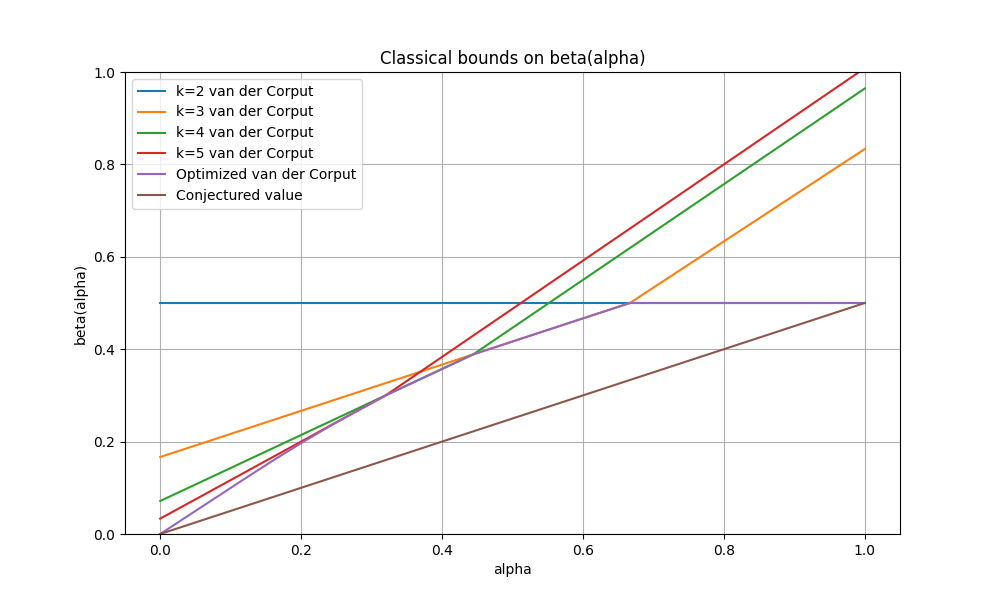
\includegraphics[width=0.5\linewidth]{chapter/van_der_corput_beta.png}
    \caption{The bounds in Proposition \ref{beta-vdc} for $k=2,3,4,5$, compared against the optimized bound in Corollary \ref{vdc-opt}.}
    \label{fig:vdc}
\end{figure}

\begin{figure}
    \centering
    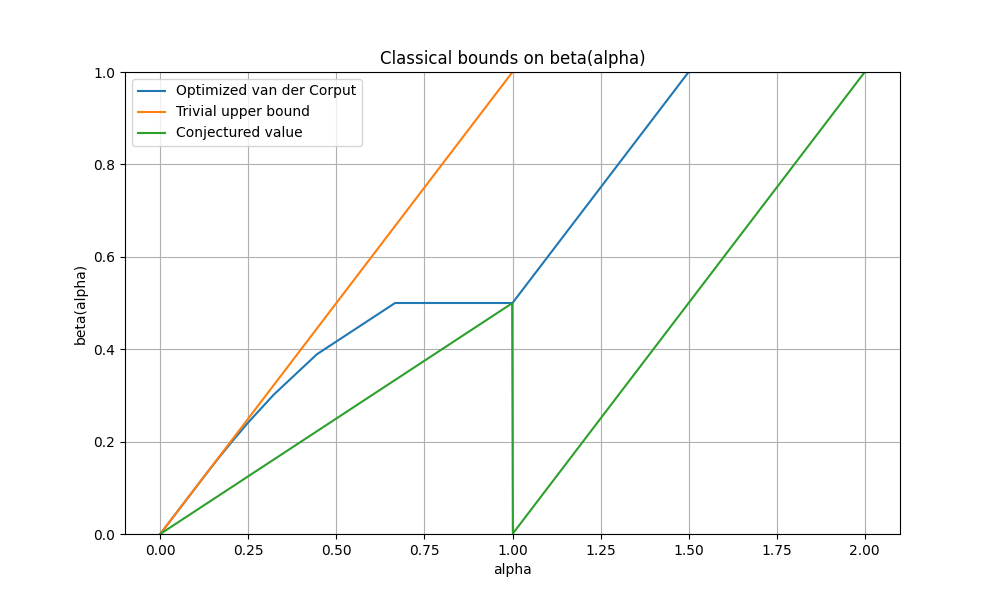
\includegraphics[width=0.5\linewidth]{chapter/van_der_corput_beta_vs_conjectured.png}
    \caption{The bound in Corollary \ref{vdc-opt}, compared against the trivial upper and lower bounds in Lemma \ref{beta-triv}.}
    \label{fig:vdc2}
\end{figure}

We remark that this corollary also follows from Proposition \ref{vdc-class}.



% Exponential sums and the Riemann zeta function II
\begin{theorem}[Watt bound]\label{beta-Watt}\uses{beta-def} For any $3/7 \le \alpha \le 1/2$, one has
    \[
    \beta(\alpha) \le \frac{89}{560} + \frac{1}{2}\alpha.
    \]
    \end{theorem}


\literature
\code{add_beta_bound_watt_1989()}

    \begin{proof}
    See \cite[Theorem~5]{watt_exponential_1989}.
    \end{proof}



% Exponential sums and the Riemann zeta function III
\begin{theorem}[1991 Huxley--Kolesnik bound]\label{beta-HK2}\uses{beta-def}  For any $2/5 \le \alpha \le 1/2$ one has
\[
\beta(\alpha) \le \max\left(\frac{1 + 8\alpha}{22}, \frac{11 + 112\alpha}{158}, \frac{1 + 17\alpha}{22}\right).
\]
\end{theorem}


\literature
\code{add_beta_bound_huxley_kolesnik_1991()}

\begin{proof}
See \cite[Theorem~3]{huxley_exponential_1991}. Note that the paper contains an error, however this result was reinstated with the corrections given in \cite{huxley_exponential_1993_1}.
\end{proof}



% Exponential sums and the Riemann zeta function IV
\begin{theorem}[1993 Huxley bound]\label{beta-Huxley-4}\uses{beta-def} For any $0 \le \alpha \le 49/114$, one has
\[
\beta(\alpha) \le \max\left(\frac{13}{60} + \frac{7}{20}\alpha, \frac{11}{120} + \frac{13}{20}\alpha\right).
\]
Furthermore, for any $49/114 \le \alpha \le 1/2$, one has
\[
\beta(\alpha) \le \frac{89}{570} + \frac{1}{2}\alpha.
\]
\end{theorem}


\literature
\code{add_beta_bound_huxley_1993()}

\begin{proof}
See \cite[Theorem~1]{huxley_exponential_1993}.
\end{proof}


\begin{theorem}[Second 1993 Huxley bound]\label{beta-Huxley-4a}\uses{beta-def} If $0 \leq \alpha \leq 1$, then $\beta(\alpha)$ is bounded by
    \begin{align*}
        \frac{1}{146} (13+94\alpha) & \hbox{ for } \alpha \leq \frac{87}{275} \\
        \frac{1}{244} (11+191\alpha) & \hbox{ for } \frac{87}{275} \leq \alpha \leq \frac{423}{1295} \\
        \frac{1}{1282} (89+908\alpha) & \hbox{ for } \frac{423}{1295} \leq \alpha \leq \frac{227}{601} \\
        \frac{1}{280} (29+173\alpha) & \hbox{ for } \frac{227}{601} \leq \alpha \leq \frac{12}{31} \\
        \frac{1}{128} (4+103\alpha) & \hbox{ for } \frac{12}{31} \leq \alpha \leq 1.
    \end{align*}
\end{theorem}


\literature
\code{add_beta_bound_huxley_1993_3()}

\begin{proof}
See \cite[Theorem~3]{huxley_exponential_1993}.
\end{proof}


\begin{theorem}[1995 Sargos bound]\label{sargos_1995}\cite[Th\'eor\`eme 2.4, Lemme 2.6]{sargos_points_1995}  For any $0 \leq \alpha \leq 1$, one has
$$ \beta(\alpha) \leq \max\left(\alpha + \frac{3(1-4\alpha)}{40}, \frac{7}{8} \alpha, \frac{1}{3}\alpha - \frac{1-4\alpha}{6}, 0\right)$$
and
$$ \beta(\alpha) \leq \max\left(\alpha + \frac{1-4\alpha}{14}, \frac{5}{6} \alpha, \frac{1}{3}\alpha - \frac{1-4\alpha}{6}, 0\right).$$
\end{theorem}

\literature
\code{add_beta_bound_sargos_1995()}

\begin{table}[ht]
    \caption{Huxley table 17.1.}
    \centering
    \renewcommand{\arraystretch}{1.2}
    \begin{tabular}{|c|c|c|}
    \hline
    $\beta_0(\alpha)$  & $X$ & $Y$ \\
    \hline
    $\frac{4+39\alpha}{60}$ & $\frac{7}{12}$ & $\frac{517}{873} = 0.5922\dots$ \\
    \hline
    $\frac{29+42\alpha}{120}$ & $\frac{65}{114}$ & $\frac{7}{12} = 0.5833\dots$ \\
    \hline
    $\frac{89+285\alpha}{570}$ & $\frac{49}{114}$ & $\frac{65}{114} = 0.5701\dots$ \\
    \hline
    $\frac{11+78\alpha}{120}$ & $\frac{5}{12}$ & $\frac{49}{114} = 0.4298\dots$ \\
    \hline
    $\frac{13+21\alpha}{60}$ & $\frac{356}{873}$ & $\frac{5}{12} = 0.4166\dots$ \\
    \hline
    $\frac{4+103\alpha}{128}$ & $\frac{12}{31}$ & $\frac{356}{873} = 0.4546\dots$ \\
    \hline
    $\frac{29+173\alpha}{280}$ & $\frac{227}{601}$ & $\frac{12}{31} = 0.3870\dots$ \\
    \hline
    $\frac{89+908\alpha}{1282}$ & $\frac{423}{1295}\dots$ & $\frac{227}{601} = 0.3777\dots$ \\
    \hline
    $\frac{11+191\alpha}{244}$ & $\frac{87}{275}$ & $\frac{423}{1295} = 0.3266\dots$ \\
    \hline
    $\frac{13+94\alpha}{146}$ & $\frac{1424}{4747}$ & $\frac{87}{275} = 0.3163\dots$\\
    \hline
    $\frac{4+235\alpha}{264}$ & $\frac{120}{419}$ & $\frac{1424}{4747}=0.2999\dots$ \\
    \hline
    $\frac{49+1351\alpha}{1614}$ & $\frac{967}{3428}$ & $\frac{120}{419} = 0.2863\dots$ \\
    \hline
    $\frac{29+464\alpha}{600}$ & $\frac{199}{716}$ & $\frac{967}{3428} = 0.2820\dots$ \\
    \hline
    $\frac{89+2243\alpha}{2706}$ & $\frac{19}{74}$ & $\frac{199}{716} = 0.2779\dots$ \\
    \hline
    $\frac{11+428\alpha}{492}$ & $\frac{161}{646}$ & $\frac{19}{74} = 0.2567\dots$ \\
    \hline
    $\frac{13+253\alpha}{318}$ & $\frac{2848}{12173} =0.2339\dots$ & $\frac{161}{646} = 0.2492\dots$ \\
    \hline
    \end{tabular}
    \end{table}\label{huxley-table-1}

    \begin{table}[ht]
        \caption{Huxley table 19.1.}
        \centering
        \renewcommand{\arraystretch}{1.2}
        \begin{tabular}{|c|c|c|}
        \hline
        $\beta_0(\alpha)$  & $X$ & $Y$ \\
        \hline
        $\frac{89+285\alpha}{570}$ & $\frac{106822}{246639}$ & $\frac{139817}{246639}=0.5668\dots$ \\
        \hline
        $\frac{2387+17972\alpha}{27290}$ & $\frac{675}{1574}$ & $\frac{106822}{246639}=0.4331\dots$ \\
        \hline
        $\frac{2819+19177\alpha}{29855}$ & $\frac{699371}{1647930}$ & $\frac{675}{1574}=0.4288\dots$ \\
        \hline
        $\frac{11897+88442\alpha}{134680}$ & $\frac{156527}{370694}$ & $\frac{699371}{1647930}=0.4243\dots$ \\
        \hline
        $\frac{113+897\alpha}{1345}$ & $\frac{263}{638}$ & $\frac{156527}{370694} = 0.4222\dots$ \\
        \hline
        $\frac{491+3624\alpha}{5530}$ & $\frac{143}{349}$ & $\frac{263}{638} = 0.4122\dots$ \\
        \hline
        $\frac{569+1053\alpha}{2800}$ & $\frac{307}{761}$ & $\frac{143}{349} = 0.4097\dots$ \\
        \hline
        $\frac{1273+2484\alpha}{6410}$ & $\frac{68682}{171139}$ & $\frac{307}{761} = 0.4034\dots$ \\
        \hline
        $\frac{4+103\alpha}{128}$ & $\frac{12}{31}$ & $\frac{68682}{171139}=0.4013\dots$ \\
        \hline
        $\frac{29+173\alpha}{280}$ & $\frac{227}{601}=0.3777\dots$ & $\frac{12}{31} = 0.3870\dots$ \\
        \hline
        \end{tabular}
\end{table}\label{huxley-table-2}


% Area, Lattice points and Exponential sums
\begin{theorem}[1996 Huxley table]\label{huxley-table}\uses{beta-def}  One can bound $\beta(\alpha)$ by $\beta_0(\alpha)$ for $X \leq \alpha \leq Y$ for $\beta_0, X, Y$ given by Tables \ref{huxley-table-1}, \ref{huxley-table-2}.
\end{theorem}


\literature
\code{add_beta_bound_huxley_1996()}\\
\code{add_beta_bound_huxley_1996_2()}

\begin{proof} See \cite[Table 17.1, Table 19.2]{huxley_area_1996} (and also \cite[\S 3.0.2, 3.0.3]{trudgian-yang} for some verification of the technical conditions on the phase).
\end{proof}


    % Exponential sums with a large second derivative
    \begin{theorem}[2001 Huxley--Kolesnik bound]\label{beta-HK}\uses{beta-def}  For any $2/5 \le \alpha \le 1/2$ one has
        $$ \beta(\alpha) \leq \max\left(\frac{7}{80} + \frac{79}{120}\alpha, \frac{3}{32} + \frac{103}{160}\alpha, \frac{9}{40} + \frac{13}{40}\alpha\right).$$
    \end{theorem}

\literature
\code{add_beta_bound_huxley_kolesnik_2001()}

    \begin{proof}
    See \cite[Theorem~1]{huxley_exponential_2001}.
    \end{proof}


%  A Fourth Derivative Test for Exponential Sums
\begin{theorem}[Robert--Sargos bound]\label{beta-RS}\uses{beta-def}  For any $\alpha > 0$ one has
    $$ \beta(\alpha) \leq \max\left( \alpha + \frac{1-4\alpha}{13}, -\frac{7(1-4\alpha)}{13}\right).$$
\end{theorem}

\literature
\code{add_beta_bound_robert_sargos_2002()}

\begin{proof}
See \cite[Theorem~1]{robert_fourth_2002}.
\end{proof}


% An analog of van der Corput’s A4-process for exponential sums
\begin{theorem}[Sargos 2003 bound]\label{sargos-bound}\uses{beta-def}  For any $\alpha > 0$ one has
$$ \beta(\alpha) \leq \max\left( \alpha + \frac{1-8\alpha}{204}, -\frac{95(1-8\alpha)}{204}\right)$$
and
$$ \beta(\alpha) \leq \max\left( \alpha + \frac{7(1-9\alpha)}{2640}, -\frac{1001(1-9\alpha)}{2640}\right).$$
\end{theorem}

\literature
\code{add_beta_bound_sargos_2003()}

\begin{proof}
See \cite[Theorems~3, 4]{sargos_analog_2003}.
\end{proof}


% Exponential sums and the Riemann zeta function VI
\begin{theorem}[Huxley bound]\label{beta-Huxley-5}\uses{beta-def} For any $1/3 \le \alpha \le 1/2$, one has
\[
\beta(\alpha) \le \max\left(\frac{37 + 59\alpha}{170}, \frac{63 + 449\alpha}{690}\right).
\]
\end{theorem}

\literature
\code{add_beta_bound_huxley_2005()}

\begin{proof}
See \cite[Proposition~1, Theorem~1]{huxley_exponential_2005}.
\end{proof}


% On the fourth derivative test for exponential sums
\begin{theorem}[Robert bound]\label{beta-R}\uses{beta-def} For any $0 < \alpha \le 3/7$ one has
\[
\beta(\alpha) \le \max\left(\alpha + \frac{1 - 4\alpha}{12}, \frac{11}{12}\alpha\right).
\]
\end{theorem}


\literature
\code{add_beta_bound_robert_2016()}

\begin{proof}
See \cite[Theorem~1]{robert_fourth_2016}.
\end{proof}

\begin{theorem}[Second Robert bound]\label{beta-R2}\uses{beta-def} If $k \geq 4$ and $\alpha \geq -(1-k\alpha) \frac{k-1}{2k-3}$ then
$$ \beta(\alpha) \leq \alpha + \max( \frac{1-k\alpha}{2(k-1)(k-2)}, -\frac{1}{2(k-1)(k-2)}).$$
\end{theorem}

\literature
\code{add_beta_bound_robert_2016_2(Constants.BETA_TRUNCATION)}

\begin{proof} See \cite[Theorem 10]{robert_2016}.
\end{proof}


\begin{theorem}[Heath-Brown bound]\label{beta-HB}\uses{beta-def}  For any $\alpha > 0$ and any natural number $k \geq 3$ one has
$$ \beta(\alpha) \leq \alpha + \max\left( \frac{1-k\alpha}{k(k-1)}, -\frac{\alpha}{k(k-1)}, -\frac{2\alpha}{k(k-1)} - \frac{2(1-k\alpha)}{k^2(k-1)}\right).$$
\end{theorem}

\literature
\code{add_beta_bound_heath_brown_2017(Constants.BETA_TRUNCATION)}

\begin{proof}
See \cite[Theorem~1]{heathbrown_new_2017}.
\end{proof}


\begin{theorem}[Bourgain bound]\label{beta-Bourgain}\uses{beta-def} One has
\[
\beta(\alpha) \le \begin{cases}
\displaystyle\frac{2}{9} + \frac{1}{3}\alpha,&\displaystyle\frac{1}{3} < \alpha \le \frac{5}{12},\\
\\
\displaystyle\frac{1}{12} + \frac{2}{3}\alpha,&\displaystyle\frac{5}{12} < \alpha \le \frac{3}{7},\\
\\
\displaystyle\frac{13}{84} + \frac{1}{2}\alpha,&\displaystyle\frac{3}{7} < \alpha \le \frac{1}{2}.
\end{cases}
\]
\end{theorem}

\literature
\code{add_beta_bound_bourgain_2017()}

\begin{proof}
See \cite[Equation~(3.18)]{bourgain_decoupling_2017}.
\end{proof}

\begin{theorem}[Heath-Brown 2020 bound]\label{beta-hb-2020}\uses{beta-def}\cite[Theorem 11.2]{demeter_small_2020}  If $\alpha$ is fixed with $1 \leq 4\alpha-1 \leq 2$ (i.e., $1/2 \leq \alpha \leq 3/4$), then
$$ \beta(\alpha) \leq \max\left( \alpha\left(1 - \frac{4\alpha-1}{4(4\alpha-1)+8}\right), \frac{8}{9} \alpha\right).$$
\end{theorem}

{\bf TODO: implement this in python}

\begin{theorem}[Combined bound]\label{combined-bound}\uses{beta-def}  For $X \leq \alpha \leq Y$, one has $\beta(\alpha) \leq \beta_0(\alpha)$, where $\beta_0, X, Y$ are given by Table \ref{huxley_table_ranges}.
\end{theorem}

\begin{proof} See \cite[Table 3]{trudgian-yang}.
\end{proof}

\begin{table}[ht]
    \def\arraystretch{1.3}
    \centering
    \caption{Bounds on $\beta(\alpha)$ of the form $\beta(\alpha) \le \beta_0(\alpha), \;(X \le \alpha \le Y)$}
    \begin{tabular}{|c|c|c|c|}
    \hline
    $\beta_0(\alpha)$ & $X$ & $Y$ & Reference\\
    \hline
    $ \frac{13}{414} + \frac{359}{414} \alpha $ & $ 0 $ & $ \frac{2848}{12173} = 0.2339\ldots $ & Exponent pair $A^2(\frac{13}{84}, \frac{55}{84})$\\
    \hline
    $\frac{13}{318} + \frac{253}{318} \alpha$ & $\frac{2848}{12173}$ & $\frac{161}{646} = 0.2492\ldots$ & Theorem \ref{huxley-table}\\
    \hline
    $\frac{11}{492} + \frac{107}{123} \alpha$ & $\frac{161}{646}$ & $\frac{19}{74} = 0.2567\ldots$ & Theorem \ref{huxley-table}\\
    \hline
    $ \frac{89}{2706} + \frac{2243}{2706} \alpha $ & $ \frac{19}{74} $ & $ \frac{199}{716} = 0.2779\ldots $ & Theorem \ref{huxley-table}\\
    \hline
    $ \frac{29}{600} + \frac{58}{75} \alpha $ & $ \frac{199}{716} $ & $ \frac{967}{3428} = 0.2820\ldots $ & Theorem \ref{huxley-table}\\
    \hline
    $ \frac{49}{1614} + \frac{1351}{1614} \alpha $ & $ \frac{967}{3428} $ & $ \frac{120}{419} = 0.2863\ldots $ & Theorem \ref{huxley-table}\\
    \hline
    $ \frac{1}{66} + \frac{235}{264} \alpha $ & $ \frac{120}{419} $ & $ \frac{1328}{4447} = 0.2986\ldots $ & Theorem \ref{huxley-table}\\
    \hline
    $ \frac{13}{194} + \frac{139}{194} \alpha $ & $ \frac{1328}{4447} $ & $ \frac{104}{343} = 0.3032\ldots $ & Exponent pair $A(\frac{13}{84}, \frac{55}{84})$\\
    \hline
    $ \frac{13}{146} + \frac{47}{73} \alpha $ & $ \frac{104}{343} $ & $ \frac{87}{275} = 0.3163\ldots $ & Theorem \ref{huxley-table}\\
    \hline
    $ \frac{11}{244} + \frac{191}{244} \alpha $ & $ \frac{87}{275} $ & $ \frac{423}{1295} = 0.3266\ldots $ & Theorem \ref{huxley-table}\\
    \hline
    $ \frac{89}{1282} + \frac{454}{641} \alpha $ & $ \frac{423}{1295} $ & $ \frac{227}{601} = 0.3777\ldots $ & Theorem \ref{huxley-table}\\
    \hline
    $ \frac{29}{280} + \frac{173}{280} \alpha $ & $ \frac{227}{601} $ & $ \frac{12}{31} = 0.3870\ldots $ & Theorem \ref{huxley-table}\\
    \hline
    $ \frac{1}{32} + \frac{103}{128} \alpha $ & $ \frac{12}{31} $ & $ \frac{1508}{3825} = 0.3942\ldots $ & Theorem \ref{huxley-table}\\
    \hline
    $ \frac{18}{199} + \frac{521}{796} \alpha $ & $ \frac{1508}{3825} $ & $ \frac{62831}{155153} = 0.4049\ldots $ & Exponent pair $D(\frac{13}{84}, \frac{55}{84})$\\
    \hline
    $ \frac{569}{2800} + \frac{1053}{2800} \alpha $ & $ \frac{62831}{155153} $ & $ \frac{143}{349} = 0.4097\ldots $ & Theorem \ref{huxley-table}\\
    \hline
    $ \frac{491}{5530} + \frac{1812}{2765} \alpha $ & $ \frac{143}{349} $ & $ \frac{263}{638} = 0.4122\ldots $ & Theorem \ref{huxley-table}\\
    \hline
    $ \frac{113}{1345} + \frac{897}{1345} \alpha $ & $ \frac{263}{638} $ & $ \frac{1673}{4038} = 0.4143\ldots $ &Theorem \ref{huxley-table}\\
    \hline
    $ \frac{2}{9} + \frac{1}{3} \alpha $ & $ \frac{1673}{4038} $ & $ \frac{5}{12} = 0.4166\ldots $ & Theorem \ref{beta-Bourgain}\\
    \hline
    $ \frac{1}{12} + \frac{2}{3} \alpha $ & $ \frac{5}{12} $ & $ \frac{3}{7} = 0.4285\ldots $ & Theorem \ref{beta-Bourgain}\\
    \hline
    $ \frac{13}{84} + \frac{1}{2} \alpha $ & $ \frac{3}{7} $ & $ \frac{1}{2}$ & Theorem \ref{beta-Bourgain}\\
    \hline
    \end{tabular}
    \label{huxley_table_ranges}
    \end{table}
    
\literature
\code{add_beta_bound_trudgian_yang_2024()}

{\bf TODO: state the Sargos result above as a lemma and a line of python code}

{\bf TODO: provide a graphic of the best bounds available of beta, compared against the classical van der Corput bounds}

\chapter{Exponent pairs}\label{exponent-pairs-chapter}

\begin{definition}[Exponent pair]\label{exp-pair-def}\uses{phase-def}  An exponent pair is a (fixed) element $(k,\ell)$ of the triangle
\begin{equation}\label{exp-pair-triangle}
    \{ (k,\ell) \in \R^2: 0 \leq k \leq 1/2 \leq \ell \leq 1, k+\ell \leq 1 \}
\end{equation}
with the following property: for all model phase functions $F$, all $T \geq N \leq 1$, and all intervals $I \subset [N,2N]$, one has
\begin{equation}\label{ntf}
 \sum_{n \in I} e(T F(n/N)) \ll (T/N)^{k+o(1)} N^{\ell+o(1)}
\end{equation}
whenever $T \geq N \geq 1$, $I$ is an interval in $[N,2N]$, and $F \in {\mathcal U}$.
\end{definition}

\python{exponent_pair}
\code{Exp_pair}

One can formulate the notion of an exponent pair without recourse to asymptotic notation:

\begin{lemma}[Non-asymptotic definition of exponent pair]\uses{exp-pair-def}  Let $(k,\ell)$ be a fixed element of \eqref{exp-pair-triangle}.  Then the following are equivalent:
    \begin{itemize}
    \item[(i)] $(k,\ell)$ is an exponent pair.
    \item[(ii)] For every (fixed) $\eps>0$ there exist (fixed) $C, P > 0$ such that, whenever $T \geq N \geq 1$, $I \subset [N,2N]$, and $F$ is a phase function obeying \eqref{fpu-bound} for for all (fixed) $0 \leq p \leq P$ and $u \in [1,2]$, then
    $$ |\sum_{n \in I} e(T F(n/N))| \leq C (T/N)^{k+\eps} N^{\ell+\eps}.$$
   \end{itemize}
\end{lemma}

The proof of this lemma is similar to that of Lemma \ref{beta-asymp} and is omitted.

Exponent pairs are closely related to the function $\beta$ from the previous chapter:

\begin{lemma}[Duality between exponent pairs and $\beta$]\label{beta-duality}\uses{beta-def, exp-pair-def}  Let $(k,\ell)$ be in the triangle \eqref{exp-pair-triangle}.  Then the following are equivalent:
    \begin{itemize}
    \item[(i)] $(k,\ell)$ is an exponent pair.
    \item[(ii)] $\beta(\alpha) \leq k + (\ell-k)\alpha$ for all $0 \leq \alpha \leq 1$.
    \end{itemize}
    \end{lemma}

    \python{exponent_pair}
    \code{exponent_pairs_to_beta_bounds()}
    \code{beta_bounds_to_exponent_pairs()}

Thus exponent pairs are dual to the convex hull of the graph of $\beta$.  But $\beta$ is not known to be convex, so one could have bounds on $\beta$ that do not directly correspond to exponent pairs.  We remark that in the case $\ell - k \geq 1/2$, one only needs to check the case $0 \leq \alpha \leq 1/2$ in (ii) above, since the remaining regime $1/2 \leq \alpha \leq 1$ then follows from Lemma \ref{beta-reflect} and some algebra.  Conversely, if $\ell - k \geq 1/2$, one only needs to check the region $1/2 \leq \alpha \leq 1$.

\begin{proof}  If (i) holds, then for any $0 < \alpha < 1$, any unbounded $T \geq 1$, any $N = T^{\alpha+o(1)}$, interval $I \subset [N,2N]$, and model phase function $F$, we have from (i) that
$$ \sum_{n \in I} e(T F(n/N)) \ll (T/N)^{k+o(1)} N^{\ell+o(1)} = T^{k + (\ell-k)\alpha + o(1)}.$$
From Definition \ref{beta-def} we conclude that $\beta(\alpha) \leq k + (\ell-k) \alpha$.  Also since $(k,\ell)$ lies in \eqref{exp-pair-triangle}, we see from \eqref{beta-0}, \eqref{beta-1} that we also have $\beta(\alpha) \leq k + (\ell-k) \alpha$ for $\alpha=0,1$.

Now suppose that (ii) holds.  Let $F, T, N, I$ be as in Definition \ref{exp-pair-def}.  By underspill it suffices to show that
$$ \sum_{n \in I} e(T F(n/N)) \ll (T/N)^{k+\eps+o(1)} N^{\ell+\eps+o(1)}$$
for any fixed $\eps>0$.  We may assume that $T \leq N^{1/\eps+1}$, since the claim follows from the trivial bound $\sum_{n \in I} e(T F(n/N)) \ll N$ otherwise.  We may also assume that $N$ is unbounded, since the claim is clear for $N$ bounded; this forces $T$ to be unbounded as well.

By passing to a subsequence we may assume that $N = T^{\alpha+o(1)}$ for some fixed $0 \leq \alpha \leq 1$.  By Definition \ref{beta-def} we then have
$$ \sum_{n \in I} e(T F(n/N)) \ll T^{\beta(\alpha)+o(1)}$$
and hence by (ii)
$$ \sum_{n \in I} e(T F(n/N)) \ll (T/N)^{k+o(1)} N^{\ell+o(1)}$$
giving the claim.
\end{proof}


\begin{corollary}[Exponent pairs closed and convex]\label{exp-pair-closed}\uses{exp-pair-def} The set of exponent pairs is closed and convex.
\end{corollary}

\begin{proof}\uses{beta-duality} Immediate from Lemma \ref{beta-duality}.
\end{proof}

\begin{proposition}[Trivial exponent pairs]\label{exp-pair-trivial}\uses{exp-pair-def}  $(0,1)$ and $(1/2,1/2)$ are exponent pairs.
\end{proposition}

\python{exponent_pair}
\code{trivial_exp_pair}

\begin{proof}\uses{beta-duality, beta-triv} Immediate from Lemma \ref{beta-duality} and Lemma \ref{beta-triv}.
\end{proof}

\begin{conjecture}[Exponent pairs conjecture]\label{exp-pair-conj}\uses{exp-pair-def, exp-pair-closed, exp-pair-trivial}  $(0,1/2)$ is an exponent pair.  (Equivalently, by Corollary \ref{exp-pair-closed} and Proposition \ref{exp-pair-trivial}, every point in the triangle \eqref{exp-pair-triangle} is an exponent pair.)
\end{conjecture}

\python{exponent_pair}
\code{exponent_pair_conjecture}


\begin{lemma}\label{exp-pair-conj-beta}\uses{exp-pair-conj}  The exponent pair conjecture is equivalent to $\beta(\alpha)=\alpha/2$ holding true for all $0 \leq \alpha \leq 1$.
\end{lemma}

\begin{proof}\uses{beta-duality, beta-triv} Clear from Lemma \ref{beta-duality} and Lemma \ref{beta-triv}.
\end{proof}

\begin{proposition}[Van der Corput $A$-process]\label{vdc-a}  If $(k,\ell)$ is an exponent pair, then so is
    $$A(k,\ell) := \left(\frac{k}{2k+2}, \frac{\ell}{2k+2} + \frac{1}{2}\right).$$
\end{proposition}

\literature
\code{A_transform_hypothesis}

\begin{proof}\uses{vdca-beta, beta-duality} See \cite[Lemma 2.8]{ivic}. It can also be deduced from Lemma \ref{vdca-beta} and Lemma \ref{beta-duality}.
\end{proof}

\begin{proposition}[Van der Corput $B$-process]\label{vdc-b}  If $(k,\ell)$ is an exponent pair, then so is
    $$B(k,\ell) := \left(\ell-\frac{1}{2}, k+\frac{1}{2}\right).$$
\end{proposition}

\literature
\code{B_transform_hypothesis}

\begin{proof}\uses{beta-reflect, beta-duality}  See \cite[Lemma 2.9]{ivic}.  Alternatively, this can be derived from Lemma \ref{beta-reflect} and Lemma \ref{beta-duality}.
\end{proof}


\section{Known exponent pairs}


\begin{proposition}[Classical van der Corput exponent pairs]\label{vdc-class}\uses{exp-pair-def} For any natural number $k \geq 2$,
    $$ A^{k-2} B(0,1) = \left( \frac{1}{2^k-2}, 1 - \frac{k-1}{2^k-2} \right)$$
    is an exponent pair.  In particular,
    $$ \left(\frac{1}{2}, \frac{1}{2}\right), \left(\frac{1}{6}, \frac{2}{3}\right), \left(\frac{1}{14}, \frac{11}{14}\right)$$
    are exponent pairs.
    \end{proposition}

    \begin{proof}\uses{vdc-a, exp-pair-trivial, vdc-opt, beta-duality} Follows by induction from Proposition \ref{vdc-a} and Proposition \ref{exp-pair-trivial}; alternatively, follows from (and is equivalent to) Corollary \ref{vdc-opt} and Lemma \ref{beta-duality}.
    \end{proof}

\derived
\code{van_der_corput_pair()}

\begin{corollary}[Additional exponent pairs]\label{add-exponential}  The pairs
$$ \left(\frac{13}{31}, \frac{16}{31}\right), \left(\frac{4}{11},\frac{6}{11}\right), \left(\frac{2}{7},\frac{4}{7}\right), \left(\frac{5}{24},\frac{15}{24}\right), \left(\frac{4}{18},\frac{11}{18}\right)$$
are all exponent pairs.
\end{corollary}

\derived
\code{best_proof_of_exponent_pair(frac(13, 31), frac(16, 31))}
\code{best_proof_of_exponent_pair(frac(4, 11), frac(6, 11))}
\code{best_proof_of_exponent_pair(frac(2, 7), frac(4, 7))}
\code{best_proof_of_exponent_pair(frac(5, 24), frac(15, 24))}
\code{best_proof_of_exponent_pair(frac(4, 18), frac(11, 18))}

\begin{proof}\uses{vdc-a, vdc-b, exp-pair-closed, vdc-class} We have $(2/7,4/7) = BA(1/6,2/3)$, $(4/18,11/18) = BABA(1/6,2/3)$, and $(13/31, 16/31)=BAB^2A^2(1/6,2/3)$, so these cases follow from Propositions \ref{vdc-class}, \ref{vdc-a}, \ref{vdc-b}. Finally, $(4/11,6/11)$ is a convex combination of $(1/2,1/2)$ and $(2/7,4/7)$, and $(5/24, 15/24)$ is a convex combination of $(1/6,2/3)$ and $(4/18, 11/18)$, so these cases follow from Corollary \ref{exp-pair-closed}.
\end{proof}


\begin{theorem}[Exponent pairs on the line of symmetry]\label{line-sym}\uses{exp-pair-def} $(k,k+1/2)$ is an exponent pair for
\begin{itemize}
\item[(i)] $k = 9/56$ \cite[Theorem~1]{huxley_exponential_1988};
\item[(ii)] $k=89/560$ \cite[Theorem~6]{watt_exponential_1989};
\item[(iii)] $k=17/108$ \cite[p. 467]{huxley_exponential_1991};
\item[(iv)] $k=89/570$ \cite[p. 40]{huxley_exponential_1993};
\item[(v)] $k=32/205$ \cite[Theorem~1]{huxley_exponential_2005};
\item[(vi)] $k=13/84$ \cite[p. 206]{bourgain_decoupling_2017}.
\end{itemize}
\end{theorem}

\literature
\code{add_literature_exponent_pairs()}


\begin{theorem}[Exponent pairs from the Bombieri--Iwaniec method]\label{exp_pair_bombieri-iwaniec}\uses{exp-pair-def}  The following pairs are exponent pairs:
\begin{itemize}
\item[(i)] $(\frac{2}{13}, \frac{35}{52})$ \cite{huxley_watt_exponential_1990};
\item[(ii)] $(\frac{6299}{43860}, \frac{29507}{43860})$ \cite[Table 17.3]{huxley_area_1996};
\item[(iii)] $(\frac{771}{8116}, \frac{1499}{2029})$ \cite[p. 285]{sargos_points_1995};
\item[(iv)] $(\frac{21}{232}, \frac{173}{232})$ \cite[p. 286]{sargos_points_1995};
\item[(v)] $(\frac{1959}{21656}, \frac{16135}{21656})$ \cite[p. 286]{sargos_points_1995};
\item[(vi)] $(\frac{516247}{6629696}, \frac{5080955}{6629696})$ \cite{huxley_exponential_2001}, \cite[Table 19.2]{huxley_area_1996}, \cite{robert_fourth_2002}.
\end{itemize}
\end{theorem}

\literature
\code{add_literature_exponent_pairs()}

\begin{theorem}[Exponent pairs from derivative tests]\label{exp_pair_deriv_test}\uses{exp-pair-def} $(k,1-mk)$ is an exponent pair when
    \begin{itemize}
\item[(i)] $k=\frac{1}{13}$ and $m=3$ \cite[Theorem 1]{robert_fourth_2002};
\item[(ii)] $k = \frac{1}{204}$ and $m=7$ \cite[p. 231]{sargos_analog_2003};
\item[(iii)] $k = \frac{1}{130}$ and $m=8$ \cite[(1.1)]{robert_2002};
\item[(iv)] $k = \frac{7}{2640}$ and $m=8$ \cite[p. 231]{sargos_analog_2003};
\item[(v)] $k = \frac{1}{716}$ and $m=9$ \cite[p. 231]{sargos_analog_2003};
\item[(vi)] $k = \frac{1}{649}$ and $m=9$ \cite{Robert_Sargos_2001};
\item[(vii)] $k = \frac{7}{4540}$ and $m=9$ \cite[(1.2)]{robert_2002};
\item[(viii)] $k = \frac{1}{615}$ and $m=9$ \cite[(1.1)]{robert_2002};
\item[(ix)] $k = \frac{1}{915}$ and $m=10$ \cite[Th\'eor\`eme 2]{robert_2002b}.
\end{itemize}
\end{theorem}

\literature
\code{add_literature_exponent_pairs()}


\begin{theorem}[Huxley sequence]\label{huxley_exp_pair}\cite[Table 17.3]{huxley_area_1996}\uses{exp-pair-def}  For any integer $m \geq 1$, the pair
    $$ \left(\frac{169}{1424 \times 2^m - 338}, 1 - \frac{169}{1424 \times 2^m - 338} \frac{712m+1577}{712}\right)$$
is an exponent pair.
\end{theorem}

\literature
\code{add_huxley_exponent_pairs(Constants.EXP_PAIR_TRUNCATION)}

\begin{theorem}[1996 Heath--Brown sequence]\label{heath-brown_exp_pair_1996}\cite[(6.17.4)]{titchmarsh_theory_1986}\uses{exp-pair-def}  For any integer $m \geq 3$, the pair
$$ \left(\frac{1}{25m^2 (m-2) \log m}, 1 - \frac{1}{25 m^2 (m-2) \log m}\right)$$
is an exponent pair.
\end{theorem}

(Currently not implemented in python due to the irrational exponents.)

\begin{theorem}[2017 Heath--Brown sequence]\label{heath-brown_exp_pair_2017}\cite[Theorem 2]{heathbrown_new_2017}\uses{exp-pair-def}
For any integer $m \geq 3$, the pair
$$ (p_m,q_m) := \left(\frac{2}{(m-1)^2(m+2)}, 1 - \frac{3m-2}{m(m-1)(m+2)}\right)$$
is an exponent pair.
\end{theorem}

\literature
\code{add_heath_brown_exponent_pairs(Constants.EXP_PAIR_TRUNCATION)}

\begin{proof} This follows from Theorem \ref{beta-HB} and Lemma \ref{beta-duality}, after some computation.
\end{proof}


\begin{theorem}[Sargos $C$-process]\label{sargos_C}\cite[Theorem 5]{sargos_analog_2003}\uses{exp-pair-def}  If $(k,\ell)$ is an exponent pair, then so is
    $$ \left(\frac{k}{12(1+4k)}, \frac{11(1+4k)+\ell}{12(1+4k)}\right).$$
\end{theorem}

\literature
\code{C_transform_hypothesis}

The following process is not quite a process to automatically transform one exponent pair to another, but it often achieves this in practice:

\begin{theorem}[Sargos $D$-process]\label{sargos_D}\cite[Theorem 7.1]{sargos_points_1995}\uses{exp-pair-def, beta-def}  If $(k,\ell)$ is an exponent pair, then one has
    $$ \beta(\alpha) \leq \max\left( k_1 + \alpha(\ell_1-k_1), \frac{1}{12} + \frac{2}{3} \alpha\right)$$
    for all $0 \leq \alpha \leq 1$, where $(k_1,\ell_1) = D(k,\ell)$ is the pair
$$ D(k,\ell) := \left(\frac{5k+\ell+2}{8(5k+3\ell+2)}, \frac{29k+21\ell+10}{8(5k+3\ell+2)}\right).$$
\end{theorem}

\literature
\code{D_transform_hypothesis}


\begin{theorem}\label{trudgian_yang_eps}\cite[Lemma 1.1]{trudgian-yang}\uses{exp-pair-def}  The following are exponent pairs:
\begin{align*}
 (k_1,\ell_1) &:= \left(\frac{4742}{38463}, \frac{35731}{51284}\right)\\
 (k_2,\ell_2) &:= \left(\frac{18}{199}, \frac{593}{796}\right)\\
 (k_3,\ell_3) &:= \left(\frac{2779}{38033}, \frac{58699}{76066}\right)\\
 (k_4,\ell_4) &:= \left(\frac{715}{10238}, \frac{7955}{10238}\right).
\end{align*}
\end{theorem}

\literature
\code{add_literature_exponent_pairs()}

\begin{proof}\uses{line-sym, beta-duality, beta-reflect, combined-bound}  For the pair $(18/199, 593/796)$, apply Theorem \ref{sargos_D} with the pair $(13/84, 55/84)$ from Theorem \ref{line-sym} to conclude that
    $$ \beta(\alpha) \leq 18/199 + 521 \alpha / 796$$
    for all $0 \leq \alpha \leq 1/2$, from which the claim follows from Lemma \ref{beta-duality} (and Lemma \ref{beta-reflect}).
The remaining pairs come from Lemma \ref{beta-duality} and the remaining components of Theorem \ref{combined-bound}.
\end{proof}

\begin{corollary}[Set of exponent pairs]\label{H-pairs}\cite[Theorem 1.3]{trudgian-yang}\uses{exp-pair-def}  Let $H$ be the convex hull $(0,1)$, $(1/2,1/2)$, and of $(k_n,\ell_n)$ for $n \in \Z$, where $(k_0,\ell_0) := 13/84$, $(k_n,\ell_n)$ for $n=1,2,3,4$ is defined by Theorem \ref{trudgian_yang_eps}, $(k_n,\ell_n) := A(k_{n-4},\ell_{n-4})$ for $5 \leq n \leq 8$, $(k_n,\ell_n) := (p_n,q_n)$ for $n > 9$ (with $(p_n,q_n)$ defined by Theorem \ref{heath-brown_exp_pair_2017}), and $(k_{-n},\ell_{-n}) := B(k_n,\ell_n)$ for $n \geq 0$.  Then all elements of $H$ are exponent pairs.
\end{corollary}

Indeed, as of \cite{trudgian-yang} the set $H$ represented all known exponent pairs, until Theorem \ref{new-exp-pair} below.

\begin{proof}\uses{exp-pair-closed, exp-pair-trivial, trudgian_yang_eps, heath-brown_exp_pair_2017} Clear from Corollary \ref{exp-pair-closed}, Proposition \ref{exp-pair-trivial}, \ref{trudgian_yang_eps}, and Theorem \ref{heath-brown_exp_pair_2017}.
\end{proof}

The following new exponent pairs were derived using this database:

\begin{theorem}[New exponent pairs]\label{new-exp-pair}\uses{exp-pair-def} The following are exponent pairs:
\[
\left(\frac{89}{1282}, \frac{997}{1282}\right),\quad \left(\frac{652397}{9713986}, \frac{7599781}{9713986}\right),\quad \left(\frac{10769}{351096}, \frac{609317}{702192}\right),\quad \left(\frac{89}{3478}, \frac{15327}{17390}\right).
\]
\end{theorem}
\derived
\code{prove_exponent_pair(frac(89,1282), frac(997,1282))}
\code{prove_exponent_pair(frac(652397,9713986), frac(7599781,9713986))}
\code{prove_exponent_pair(frac(10769,351096), frac(609317,702192))}
\code{prove_exponent_pair(frac(89,3478), frac(15327,17390))}

\begin{proof}\uses{beta-reflect, beta-duality}
Using the bounds on $\beta(\alpha)$ collected in Table \ref{new-exp-pair-beta-bounds-table}, one may verify (after a tedious calculation) that for each of the claimed exponent pairs $(k, \ell)$ in the lemma statement, one has $\beta(\alpha) \le k + (\ell - k)\alpha$ for $0 \le \alpha \le 1/2$. The result then follows from Lemma \ref{beta-reflect} and Lemma \ref{beta-duality}.

\begin{table}[h]
\label{new-exp-pair-beta-bounds-table}
\def\arraystretch{1.8}
\centering
\caption{Bounds on $\beta(\alpha)$}
\begin{tabular}{|c|c|c|}
\hline
$\beta(\alpha)$ bound & $\alpha$ range & Reference\\
\hline
$\dfrac{1}{20} + \dfrac{3}{4}\alpha$ & $0\leq \alpha < \dfrac{1}{4}$ & Theorem \ref{beta-HB} with $k = 5$\\
\hline
$\dfrac{19}{20}\alpha$ & $\dfrac{1}{4}\leq \alpha < \dfrac{890}{3277}$ & Theorem \ref{beta-HB} with $k = 5$\\
\hline
$\dfrac{89}{2706} + \dfrac{2243}{2706}\alpha$ & $\dfrac{890}{3277}\leq \alpha < \dfrac{199}{716}$ & Table \ref{huxley-table-1}\\
\hline
$\dfrac{1}{66} + \dfrac{235}{264}\alpha$ & $\dfrac{120}{419}\leq \alpha < \dfrac{754}{2579}$ & Table \ref{huxley-table-1}\\
\hline
$\dfrac{9}{217} + \dfrac{1389}{1736}\alpha$ & $\dfrac{754}{2579}\leq \alpha < \dfrac{251324}{841245}$ & Exponent pair $(\dfrac{9}{217}, \dfrac{1461}{1736}) = AD(\dfrac{13}{84}, \dfrac{55}{84})$\\
\hline
$\dfrac{2371}{43205} + \dfrac{52209}{69128}\alpha$ & $\dfrac{251324}{841245}\leq \alpha < \dfrac{861996}{2811205}$ & \begin{tabular}{@{}c@{}}Exponent pair $(\dfrac{2371}{43205}, \dfrac{280013}{345640})$ \\
$= A(\dfrac{4742}{38463}, \dfrac{35731}{51284})$ and Theorem \ref{trudgian_yang_eps}\end{tabular}\\
\hline
$\dfrac{13}{146} + \dfrac{47}{73}\alpha$ & $\dfrac{861996}{2811205}\leq \alpha < \dfrac{87}{275}$ & Table \ref{huxley-table-1}\\
\hline
$\dfrac{11}{244} + \dfrac{191}{244}\alpha$ & $\dfrac{87}{275}\leq \alpha < \dfrac{423}{1295}$ & Table \ref{huxley-table-1}\\
\hline
$\dfrac{89}{1282} + \dfrac{454}{641}\alpha$ & $\dfrac{423}{1295}\leq \alpha < \dfrac{227}{601}$ & Table \ref{huxley-table-1}\\
\hline
$\dfrac{715}{10238} + \dfrac{3620}{5119}\alpha$ & $\dfrac{227}{601}\leq \alpha < \dfrac{227}{601}$ & \begin{tabular}{@{}c@{}}Exponent pair $(\dfrac{715}{10238}, \dfrac{7955}{10238})$  \\
in Theorem \ref{trudgian_yang_eps}\end{tabular}\\
\hline
$\dfrac{29}{280} + \dfrac{173}{280}\alpha$ & $\dfrac{227}{601}\leq \alpha < \dfrac{12}{31}$ & Table \ref{huxley-table-1}\\
\hline
$\dfrac{1}{32} + \dfrac{103}{128}\alpha$ & $\dfrac{12}{31}\leq \alpha < \dfrac{1508}{3825}$ & Table \ref{huxley-table-1}\\
\hline
$\dfrac{18}{199} + \dfrac{521}{796}\alpha$ & $\dfrac{1508}{3825}\leq \alpha < \dfrac{62831}{155153}$ & Exponent pair $(\dfrac{18}{199}, \dfrac{593}{796}) = D(\dfrac{13}{84}, \dfrac{55}{84})$\\
\hline
$\dfrac{569}{2800} + \dfrac{1053}{2800}\alpha$ & $\dfrac{62831}{155153}\leq \alpha < \dfrac{143}{349}$ & Table \ref{huxley-table-2}\\
\hline
$\dfrac{1}{12} + \dfrac{2}{3}\alpha$ & $\dfrac{5}{12}\leq \alpha < \dfrac{3}{7}$ & Theorem \ref{beta-Bourgain} \\
\hline
$\dfrac{13}{84} + \dfrac{1}{2}\alpha$ & $\dfrac{3}{7}\leq \alpha \leq \dfrac{1}{2}$ & Theorem \ref{beta-Bourgain} \\
\hline
\end{tabular}
\end{table}
\end{proof}

In summary, the current set of known exponent pairs is the convex hull with vertices $(0, 1)$, $(1/2, 1/2)$ and the points $(k_n, \ell_n)$ for $n \in \Z$ that are recorded in Table \ref{exp_pair_table}.

\begin{table}[ht]
\label{exp_pair_table}
\caption{Vertices of the convex hull of known exponent pairs.}
\centering
\renewcommand{\arraystretch}{2}
\begin{tabular}{|c|c|c|}
\hline
$n$ & $(k_n, \ell_n)$ & Reference \\
\hline
0 & $\left(\dfrac{13}{84}, \dfrac{55}{84}\right)$ & \cite[p. 307]{bourgain_decoupling_2017} \\
\hline
1 & $\left(\dfrac{4742}{38463}, \dfrac{35731}{51284}\right)$ & Theorem \ref{trudgian_yang_eps} \\
\hline
2 & $\left(\dfrac{18}{199}, \dfrac{593}{796}\right)$ & Theorem \ref{trudgian_yang_eps} \\
\hline
3 & $\left(\dfrac{2779}{38033}, \dfrac{58699}{76066}\right)$ & Theorem \ref{trudgian_yang_eps} \\
\hline
4 & $\left(\dfrac{89}{1282}, \dfrac{997}{1282}\right)$ & Theorem \ref{new-exp-pair} \\
\hline
5 & $\left(\dfrac{652397}{9713986}, \dfrac{7599781}{9713986}\right)$ & Theorem \ref{new-exp-pair} \\
\hline
6 & $\left(\dfrac{2371}{43205}, \dfrac{280013}{345640}\right)$ & $A(k_1, \ell_1)$ \\
\hline
7 & $\left(\dfrac{9}{217}, \dfrac{1461}{1736}\right)$ & $A(k_2, \ell_2)$\\
\hline
8 & $\left(\dfrac{10769}{351096}, \dfrac{609317}{702192}\right)$ & Theorem \ref{new-exp-pair} \\
\hline
9 & $\left(\dfrac{89}{3478}, \dfrac{15327}{17390}\right)$ & Theorem \ref{new-exp-pair} \\
\hline
$n \ge 10$ & \begin{tabular}{@{}c@{}}$(p_{n + 4}, q_{n + 4})$, where \\
$(p_m, q_m) = \left(\dfrac{2}{(m-1)^2(m+2)}, 1 - \dfrac{3m-2}{m(m-1)(m+2)}\right)$\end{tabular} & Theorem \ref{heath-brown_exp_pair_2017} \\
\hline
$n < 0$ & $B(k_{-n}, \ell_{-n})$ & Proposition \ref{vdc-b} \\
\hline
\end{tabular}
\end{table}


\begin{figure}
    \centering
    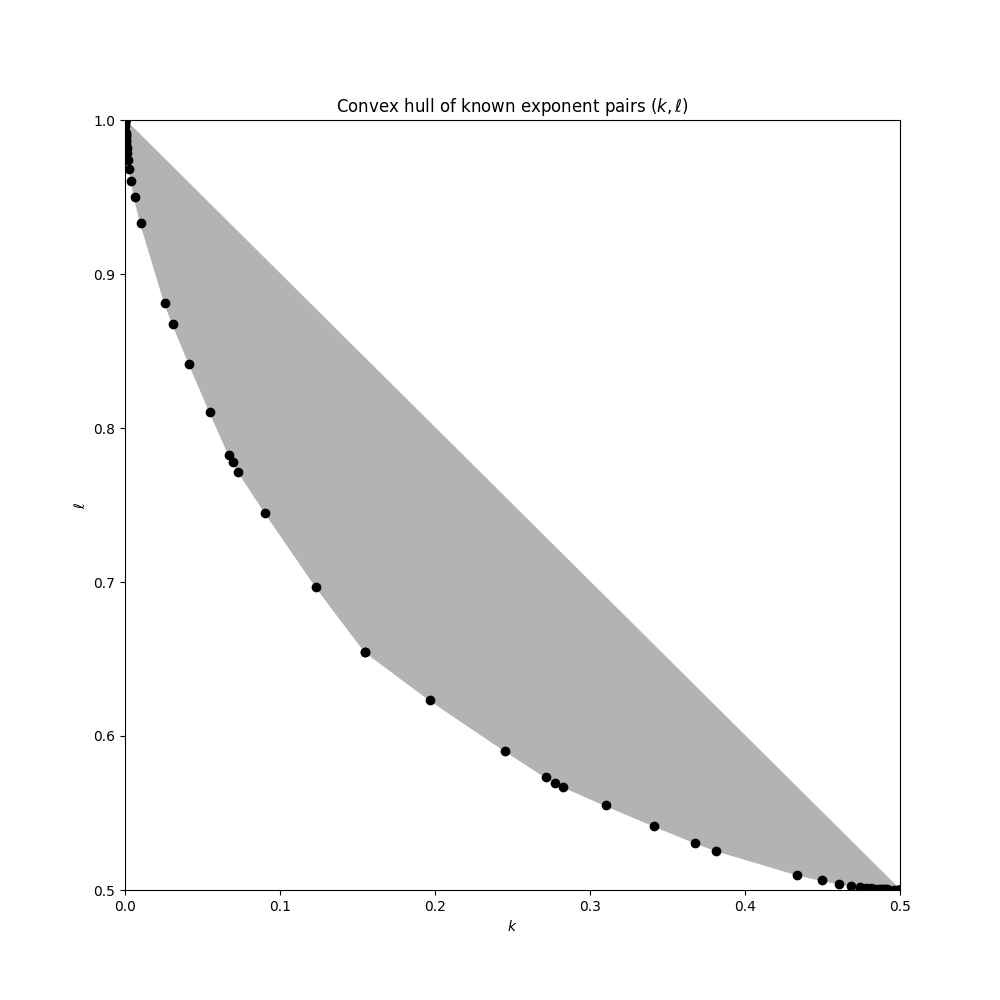
\includegraphics[width=0.5\linewidth]{chapter/exp_pair_plot.png}
    \caption{The convex hull of known exponent pairs, whose vertices $(k_n, \ell_n)$ are given in Table \ref{exp_pair_table}.}
    \label{fig:exp_pair_plot}
\end{figure}

\chapter{Growth exponents for the Riemann zeta function}\label{zeta-growth-chapter}

\begin{definition}[Growth rate of zeta]\label{zeta-grow-def}  For any fixed $\sigma \in \R$, let $\mu(\sigma)$ denote the least possible (fixed) exponent for which one has the bound
    $$ |\zeta(\sigma+it)| \ll |t|^{\mu(\sigma)+o(1)}$$
    for all unbounded $t$.
\end{definition}

One can check that for each $\sigma$, the set of possible candidates for $\mu(\sigma)$ is closed (by underspill), non-empty, and bounded from below, so that $\mu(\sigma)$ is well-defined as a real number.  An equivalent definition without asymptotic notation, is that $\mu(\sigma)$ is the least real number such that for every $\eps>0$ there exists $C>0$ such that
$$ |\zeta(\sigma+it)| \leq C |t|^{\mu(\sigma)+\eps}$$
for all $t$ with $|t| \geq C$; equivalently, one has
$$ \mu(\sigma) = \limsup_{|t| \to \infty} \frac{\log |\zeta(\sigma+it)|}{\log|t|}.$$

\python{bound_mu}
\code{Bound_mu}

\begin{lemma}[Trivial bound]\label{zeta-grow-triv}\uses{zeta-grow-def}
    One has $\mu(\sigma)=0$ for all $\sigma \geq 1$.
\end{lemma}

\python{bound_mu}
\code{apply_trivial_mu_bound()}

\begin{proof}  Immediate from the absolute convergence of the Dirichlet series for both $\zeta(s)$ and $1/\zeta(s)$; see e.g., \cite[Theorem 1.9]{ivic}.
\end{proof}

\begin{lemma}[Convexity]\label{zeta-convex}\uses{zeta-grow-def}
$\mu$ is convex.
\end{lemma}

\python{bound_mu}
\code{bound_mu_convexity()}

\begin{proof} Immediate from the Phragm\'en--Lindel\"of principle; see e.g., \cite[\S A.8]{ivic}.
\end{proof}

\begin{lemma}[Functional equation]\label{zeta-functional}\uses{zeta-grow-def}
    One has $\mu(1-\sigma) = \mu(\sigma) + \sigma - 1/2$ for all $0 \leq \sigma \leq 1/2$.
\end{lemma}

\python{bound_mu}
\code{apply_functional_equation()}

\begin{proof}  Immediate from the functional equation for $\zeta$ and asymptotics of the Gamma function; see e.g., \cite[(1.23), (1.25)]{ivic}.
\end{proof}

\begin{lemma}[Left of critical strip]\label{zeta-left}\uses{zeta-grow-def}
    One has $\mu(\sigma)=1/2-\sigma$ for $\sigma \leq 0$.
\end{lemma}

\python{bound_mu}
\code{apply_trivial_mu_bound()}

\begin{proof}\uses{zeta-grow-triv, zeta-functional}  Immediate from Lemmas \ref{zeta-grow-triv}, \ref{zeta-functional}.
\end{proof}

\begin{lemma}[Convexity bounds]\label{zeta-convexity}\uses{zeta-grow-def}  One has $\max(0, 1/2-\sigma) \leq \mu(\sigma) \leq (1-\sigma)/2$ for $0 \leq \sigma \leq 1$.
\end{lemma}

\python{bound_mu}
\code{apply_trivial_mu_bound()}

\begin{proof}\uses{zeta-grow-triv, zeta-convex, zeta-left}  Immediate from Lemma \ref{zeta-grow-triv}, Lemma \ref{zeta-left}, and Lemma \ref{zeta-convexity}.
\end{proof}

\section{Connection with exponent pairs and dual exponent pairs}

\begin{lemma}[Connection with dual exponent pairs]\label{mu-beta}\label{zeta-grow-def, beta-def}  For any $1/2 \leq \sigma \leq 1$, one has
    $$ \mu(\sigma) \leq \sup_{0 \leq \alpha \leq 1/2} \beta(\alpha) - \alpha \sigma.$$
\end{lemma}

\begin{proof}\uses{auto}  Let $t$ be unbounded.  From the Riemann--Siegel formula (see \cite[Theorem 4.1]{ivic}) one has
    $$ \zeta(\sigma+it) \ll \left|\sum_{n \leq \sqrt{t/2\pi}} \frac{1}{n^{\sigma+it}}\right| + |t|^{1/2-\sigma} \left|\sum_{n \leq \sqrt{t/2\pi}} \frac{1}{n^{1-\sigma-it}}\right| + O(1).$$
From dyadic decomposition and Definition \ref{beta-def} (and Lemma \ref{auto}) one has for any fixed $\eps>0$ that
$$\sum_{t^\eps \leq n \leq \sqrt{t/2\pi}} \frac{1}{n^{\sigma+it}} \ll
|t|^{\sup_{\eps \leq \alpha \leq 1/2} \beta(\alpha) - \alpha \sigma + o(1)},$$
while from the triangle inequality one has the crude bound
$$\sum_{n < t^\eps} \frac{1}{n^{\sigma+it}} \ll |t|^\eps.$$
Combining the bounds and using underspill, we conclude that
$$\sum_{n \leq \sqrt{t/2\pi}} \frac{1}{n^{\sigma+it}} \ll
|t|^{\sup_{0 \leq \alpha \leq 1/2} \beta(\alpha) - \alpha \sigma + o(1)}.$$
A similar argument gives
$$\sum_{n \leq \sqrt{t/2\pi}} \frac{1}{n^{1-\sigma-it}} \ll
|t|^{\sup_{0 \leq \alpha \leq 1/2} \beta(\alpha) - \alpha (1-\sigma) + o(1)}$$
Since $\sigma \geq 1/2$ and $\alpha \leq 1/2$, one has $(1/2-\sigma) - \alpha(1-\sigma) \leq -\alpha \sigma$, and hence
$$ \zeta(\sigma+it) \ll
|t|^{\sup_{0 \leq \alpha \leq 1/2} \beta(\alpha) - \alpha \sigma + o(1)}$$
giving the claim.
\end{proof}

We remark that this inequality is morally an equality (indeed, it would be if one would restrict the model phases in Definition \ref{beta-def} to purely the logarithmic phase $u \mapsto \log u$).

The following form of Lemma \ref{mu-beta} is convenient for applications:

\begin{corollary}[Exponent pairs and $\mu$]\label{exp-pair-mu}\uses{exp-pair-def, zeta-grow-def} If $(k,\ell)$ is an exponent pair, then
$$ \mu(\ell-k) \leq k.$$
\end{corollary}

\python{bound_mu}
\code{obtain_mu_bound_from_exponent_pair()}

\begin{proof}\uses{mu-beta, beta-duality}  Immediate from Lemma \ref{mu-beta} and Lemma \ref{beta-duality}.  See also \cite[(7.57)]{ivic}.
\end{proof}

\begin{conjecture}[Lindel\"of hypothesis]\label{LH}\uses{zeta-grow-def} One has $\mu(1/2)=0$.
\end{conjecture}

\python{bound_mu}
\code{bound_mu_Lindelof()}

\begin{lemma}\label{exp-pair_implies_lindelof}\uses{exp-pair-conj, LH}  The exponent pair conjecture implies the Lindel\"of hypothesis.
\end{lemma}

\begin{proof}\uses{exp-pair-mu} Immediate from Corollary \ref{exp-pair-mu}.
\end{proof}

\begin{proposition}[Conjectured value of $\mu$]\label{mu-conj}\uses{zeta-grow-def, LH}  We have the lower bound
\begin{equation}\label{muh}
    \mu(\sigma) \geq \max\left(0, \frac{1}{2}-\sigma\right)
\end{equation}
for all $\sigma \in \R$, and equality holds everywhere in \eqref{muh} if and only if the Lindel\"of hypothesis holds.
\end{proposition}

We remark that this proposition explains why there are no further lower bounds on $\mu$ in the literature beyond \eqref{muh}; all the remaining known results revolve around upper bounds.

\begin{proof}\uses{zeta-grow-triv, zeta-left, zeta-convexity}  Clearly equality in \eqref{muh} implies the Lindel\"of hypothesis, while from the trivial bounds in Propositions \ref{zeta-grow-triv}, \ref{zeta-left} and convexity (Lemma \ref{zeta-convexity}) one we see that the Lindel\"of hypothesis implies the upper bound
$$     \mu(\sigma) \leq \max\left(0, \frac{1}{2}-\sigma\right)$$
for all $\sigma$.  So it suffices to establish the lower bound unconditionally.  By the functional equation (Proposition \ref{zeta-functional}) it suffices to do this for $\sigma \geq 1/2$; in fact by convexity it suffices to establish the claim when $1/2 < \sigma < 1$.  In this regime, the $L^2$ mean value theorem (see \cite[Theorem 1.11]{ivic}) gives
$$ \int_0^T |\zeta(\sigma+it)|^2\ dt \asymp T$$
for large $T$, giving the claim.
\end{proof}

\section{Known bounds on \texorpdfstring{$\mu$}{mu}}

\begin{theorem}[Historical bounds]\label{mu-hist}\uses{zeta-grow-def}  The upper bounds on $\mu(\sigma)$ given by Table \ref{mu-table} are known.
\end{theorem}

\begin{table}[ht]
\caption{Historical bounds on $\mu(\sigma)$ for $1/2 \le \sigma \le 1$, and the exponent pair generating them (if applicable). \textbf{Longer term goal: supplement as many of these citations as possible with derivations from other exponents and relations in the database}}
\centering
\renewcommand{\arraystretch}{1.2}
\begin{tabular}{|c|c|c|}
\hline
Reference & Results & Exponent pair \\
\hline
Hardy--Littlewood (1923) \cite{hardy_littlewood_1923} & $\mu(1/2) \le 1/6$ & (1/6, 2/3)\\
\hline
Walfisz (1924) \cite{walfisz_1924} & $\mu(1/2) \le 193/988$ & \\
\hline
Titchmarsh (1932) \cite{titchmarsh_van_1931} & $\mu(1/2) \leq 27/164$ & \\
\hline
Phillips (1933) \cite{phillips_zeta_1933} & $\mu(1/2) \leq 229/1392$ & \\
\hline
Titchmarsh (1942) \cite{titchmarsh_order_1942}  & $\mu(1/2) \leq 19/116$ & \\
\hline
Min (1949) \cite{min_on_1949} & $\mu(1/2) \leq 15/92$ & \\
\hline
Haneke (1962) \cite{haneke_verscharfung_1963} & $\mu(1/2) \leq 6/37$&  \\
\hline
Kolesnik (1973) \cite{kolesnik_1973} & $\mu(1/2) \leq 173/1067$ & \\
\hline
Kolesnik (1982) \cite{kolesnik_order_1982} & $\mu(1/2) \leq 35/216$ & \\
\hline
Kolesnik (1985) \cite{kolesnik_1985} & $\mu(1/2) \leq 139/858$ & \\
\hline
Bombieri--Iwaniec (1985) \cite{bombieri_order_1986} & $\mu(1/2) \leq 9/56$ & $(9/56, 1/2+9/56)$\\
\hline
Watt (1989) \cite{watt_exponential_1989} & $\mu(1/2) \leq 89/560$ & $(89/560, 1/2+89/560)$\\
\hline
Huxley--Kolesnik (1991) \cite{huxley_exponential_1991} & $\mu(1/2) \leq 17/108$ & $(17/108, 1/2+17/108)$\\
\hline
Huxley (1993) \cite{huxley_exponential_1993} & $\mu(1/2) \leq 89/570$ & $(89/570, 1/2+89/570)$\\
\hline
Huxley (1996) \cite{huxley_area_1996} & $\mu(1934/3655) \leq 6299/43860$ & \\
\hline
Sargos (2003) \cite{sargos_analog_2003} & $\mu(49/51) \leq 1/204$, $\mu(361/370) \leq 1/370$&  \\
\hline
Huxley (2005) \cite{huxley_exponential_2005} & $\mu(1/2) \leq 32/205$ & $(32/205, 1/2+32/205)$ \\
\hline
Lelechenko (2014) \cite{Lelechenko_linear_2014} & $\mu(3/5) \leq 1409/12170$, $\mu(4/5) \leq 3/71$& \\
\hline
Bourgain (2017) \cite{bourgain_decoupling_2017} & $\mu(1/2) \leq 13/84$ & $(13/84, 1/2+13/84)$ \\
\hline
Heath-Brown (2017) \cite{heathbrown_new_2017} & $\mu(\sigma) \le \frac{8}{63}\sqrt{15}(1 - \sigma)^{3/2}$ for $1/2 \le \sigma \le 1$& \\
\hline
Heath-Brown (2020) \cite{demeter_small_2020} & $\mu(11/15) \leq 1/15$& \\
\hline
\end{tabular}
\end{table}\label{mu-table}

\literature
\code{add_literature_bounds_mu()}


\begin{theorem}\label{mu_est_thm}\cite[Theorems 2.4-2.6]{trudgian-yang}\uses{zeta-grow-def}
    We have
    \[
    \mu(\sigma) \le \begin{cases}
         (31 - 36\sigma)/84 , & \frac{1}{2} \leq\sigma < \frac{88225}{153852} = 0.5734\ldots, \\
         (220633 - 251324\sigma)/620612 , & \frac{88225}{153852} \leq\sigma < \frac{521}{796} = 0.6545\ldots, \\
         (1333 - 1508\sigma)/3825 , & \frac{521}{796} \leq\sigma < \frac{53141}{76066} = 0.6986\ldots, \\
         (405 - 454\sigma)/1202 , & \frac{53141}{76066} \leq\sigma < \frac{3620}{5119} = 0.7071\ldots, \\
         (49318855 - 52938216\sigma)/170145110 , & \frac{3620}{5119} \leq\sigma < \frac{52209}{69128} = 0.7552\ldots, \\
         (471957 - 502648\sigma)/1682490 , & \frac{52209}{69128} \leq\sigma < \frac{1389}{1736} = 0.8001\ldots, \\
         (2841 - 3016\sigma)/10316 , & \frac{1389}{1736} \leq\sigma < \frac{134765}{163248} = 0.8255\ldots, \\
         (859 - 908\sigma)/3214 , & \frac{134765}{163248} \leq\sigma < \frac{18193}{21906} = 0.8305\ldots, \\
         5(8707 - 9067\sigma)/180277 , & \frac{18193}{21906} \leq\sigma < \frac{249}{280} = 0.8892\ldots, \\
         (29 - 30\sigma)/130 , & \frac{249}{280} \leq\sigma \leq \frac{9}{10}.\\
    \end{cases}
    \]
    Furthermore, for $1/2 \le \sigma \le 1$, we have
\[
\mu(\sigma) \le \frac{2}{13}\sqrt{10}(1 - \sigma)^{3/2} = 0.4865\ldots(1 - \sigma)^{3/2},
\]
and
\[
\mu(\sigma) \le \frac{2}{3^{3/2}}(1 - \sigma)^{3/2} + \frac{103}{300}(1 - \sigma)^{2},\qquad \frac{117955}{118272} \le \sigma \le 1.
\]
\end{theorem}

{\bf TODO: make a python function for the first part of this theorem at least.}

\chapter{Large value estimates}

\begin{definition}[Large value exponent]\label{lv-def} Let $1/2 \leq \sigma \leq 1$ and $\tau \geq 0$ be fixed. We define $\LV(\sigma,\tau)$ to be the least fixed quantity for which the following claim is true: whenever $N > 1$ is unbounded, $T = N^{\tau+o(1)}$, $V = N^{\sigma+o(1)}$, $a_n$ is a $1$-bounded complex number for each $n \in [N,2N]$, and $t_1,\dots,t_R$ are a $1$-separated sequence in some interval $J$ of length $T$ such that
\begin{equation}\label{V-large}
    \left|\sum_{n \in [N,2N]} a_n n^{-it_r} \right| \geq V
\end{equation}
    for all $r=1,\dots,R$, then one has
$$ R \ll N^{\LV(\sigma,\tau)+o(1)}.$$
\end{definition}

\python{large_values}
\code{Large_Value_Estimate}

One can check that the set of possible candidates for $\LV(\sigma,\tau)$ is closed (by underspill), non-empty, and bounded from below, so $\LV(\sigma,\tau)$ is well-defined as a real number.  As usual, we have an equivalent non-asymptotic definition:

\begin{lemma}[Asymptotic form of large value exponent]\label{lv-asymp}\uses{lv-def} Let $1/2 \leq \sigma \leq 1$, $\tau \geq 0$, and $\rho \geq 0$ be fixed.  Then the following are equivalent:
    \begin{itemize}
    \item[(i)] $\LV(\sigma,\tau) \leq \rho$.
    \item[(ii)] For every (fixed)  $\eps>0$ there exists $C, \delta>0$ such that if $N \geq C$ and $N^{\tau-\delta} \leq T \leq N^{\tau+\delta}$, $N^{\sigma-\delta} \leq V \leq N^{\sigma+\delta}$, $a_n$ is a $1$-bounded complex number for each $n \in [N,2N]$, and $t_1,\dots,t_R$ is a $1$-separated subset of an interval $J$ of length $T$ such that \eqref{V-large} holds for all $r=1,\dots,R$, then one has
    $$ R \leq C N^{\rho+\eps}.$$
    \end{itemize}
\end{lemma}

The proof of Lemma \ref{lv-asymp} is similar to that of Lemma \ref{beta-asymp}, and is left to the reader.


\begin{lemma}[Basic properties]\label{lv-basic}\uses{lv-def}
    \begin{itemize}
        \item[(i)] (Monotonicity in $\sigma$) For any $\tau \geq 0$, $\sigma \mapsto \LV(\sigma,\tau)$ is upper semicontinuous and monotone non-increasing.
        \item[(ii)] (Huxley subdivision) For any $1/2 \leq \sigma \leq 1$ and $\tau' \geq \tau$ one has
$$ \LV(\sigma,\tau) \leq \LV(\sigma,\tau') \leq \LV(\sigma,\tau) + \tau'-\tau.$$
In particular, $\tau \mapsto \LV(\sigma,\tau)$ is Lipschitz continuous.
        \item[(iii)]  ($\tau=0$ endpoint) One has $\LV(\sigma,0)=0$ for all $1/2 \leq \sigma \leq 1$, and hence by (ii) $0 \leq \LV(\sigma,\tau) \leq \tau$ for all $1/2 \leq \sigma \leq 1$ and $\tau \geq 0$.
    \end{itemize}
\end{lemma}

{\bf TODO: implement Huxley subdivision as a way to transform a large values estimate into a better estimate}

\begin{proof}\uses{auto}
All claims are clear except perhaps for the upper bound
$$ \LV(\sigma,\tau') \leq \LV(\sigma,\tau) + \tau'-\tau,$$
but this follows because any interval of length $N^{\tau'+o(1)}$ may be subdivided into $N^{\tau'-\tau+o(1)}$ intervals of length $N^{\tau+o(1)}$, so on applying Definition \ref{lv-def} to each subinterval and summing (using Lemma \ref{auto} to ensure uniformity), one obtains the claim.
\end{proof}

\begin{lemma}[Lower bound]\label{lv-lower}\uses{lv-def}  For any $1/2 < \sigma \leq 1$ and $\tau \geq 0$, one has $\LV(\sigma, \tau) \geq \min(2 - 2 \sigma,\tau)$, while for $\sigma=1/2$ one has $\LV(\sigma,\tau) = \tau$.
\end{lemma}

\begin{proof}\uses{lv-basic} In view of Lemma \ref{lv-basic}(ii), it suffices to show that $\LV(\sigma, 2-2\sigma) \geq 2-2\sigma$.  By definition, it suffices to find an unbounded $N$ and a $1$-bounded sequence $a_n$ for $n \in [N,2N]$ such that $|\sum_{n \in [N,2N]} a_n n^{-it}| \geq N^{\sigma+o(1)}$ for a $1$-separated set of $t = O(N^{2-2\sigma+o(1)})$ of cardinality $\gg N^{2-2\sigma-o(1)}$.

In the endpoint case $\sigma = 1$ one can achieve this by setting $a_n=1$ for all $n$ and taking $t=0$, so now we assume that $1/2 < \sigma<1$.

We use the probabilistic method.  We divide $[N,2N]$ into $\asymp N^{2-2\sigma}$ intervals $I$ of length $\asymp N^{2\sigma-1}$.  On each interval $I$, we choose $a_n$ to equal some randomly chosen sign $\epsilon_I \in \{-1,+1\}$, with the $\epsilon_I$ chosen independently in $I$.  If $t = o(N^{2-2\sigma})$, then $\sum_{n \in I} a_n n^{-it}$ is equal to $\epsilon_I$ times a deterministic quantity $c_{t,I}$ of magnitude $\asymp N^{2\sigma-1}$ (the point being that the phase $t \log n$ is close to constant in this range).  By the Chernoff bound, we thus see that for any such $t$, $\sum_{n \in [N,2N]} a_n n^{it}$ will have size $\gg N^{(2\sigma-1) + (2-2\sigma)/2} = N^\sigma$ with probability $\gg 1$. By linearity of expectation, we thus see that with positive probability, a $\gg 1$ fraction of integers $t$ with $t = o(N^{2-2\sigma})$ will have this property, giving the claim.

Finally, let $\sigma=1/2$.  In this case we just take each $a_n$ to be a random sign, then by the Chernoff bound one has for each $t$ that $|\sum_{n \in [N,2N]} a_n n^{it}| \asymp N^{1/2}$ with positive probability, which by linearity of expectation as before gives the lower bound $\LV(\sigma,\tau) \geq \tau$, while the upper bound is trivial from Lemma \ref{lv-basic}(iii).
\end{proof}

We conjecturally have a complete description of the function $\LV$:

\begin{conjecture}[Montgomery conjecture]\label{montgomery-conj}\uses{lv-def}  One has
    \begin{equation}\label{mont-conj}
        \LV(\sigma, \tau) \leq 2 - 2 \sigma
    \end{equation}
     for all fixed $1/2 < \sigma \leq 1$ and $\tau \geq 0$. Equivalently (by Lemma \ref{lv-basic}(ii), (iii) and Lemma \ref{lv-lower}), one has $\LV(\sigma, \tau) = \min(2 - 2 \sigma,\tau)$ for all $1/2 < \sigma \leq 1$ and $\tau \geq 0$.
\end{conjecture}

\python{large_values}
\code{montgomery_conjecture}

We refer to \cite{bourgain_montgomery_1991} for further discussion of this conjecture, including some counterexamples to strong versions of the conjecture in which certain epsilon losses are omitted.  In view of this conjecture, we do not expect any further lower bounds on $\LV(\sigma,\tau)$ to be proven, and the literature is instead focused on upper bounds.

The following application of subdivision is useful:

\begin{lemma}[Subdivision and the Montgomery conjecture]\label{montgomery-subdivide}\uses{montgomery-conj}  If $\sigma$ is fixed, and the Montgomery conjecture holds for all fixed $\tau < \tau_0$, then
\begin{equation}\label{lvt-opt}
    \LV(\sigma, \tau) \leq \max( 2 - 2 \sigma, \tau - \tau_0 + 2 - 2\sigma)
\end{equation}
for all fixed $\tau \geq 0$.
\end{lemma}

\begin{proof}\uses{lv-basic}
Clear from Lemma \ref{lv-basic}(ii).
\end{proof}


The following basic property of $\LV(\sigma,\tau)$ is extremely useful in applications:

\begin{lemma}[Raising to a power]\label{power-lemma}\uses{lv-def}  For any $1/2 \leq \sigma \leq 1$, $\tau \geq 0$, and natural number $k$, one has
    $$ \LV(\sigma, k\tau) \leq k \LV(\sigma, \tau).$$
\end{lemma}

\python{large_values}
\code{raise_to_power_hypothesis()}

\begin{proof}  Let $N$ be unbounded, let $T = N^{k\tau+o(1)}$ and $V = N^{\sigma+o(1)}$, let $a_n$ be a $1$-bounded sequence on $[N,2N]$, and let $t_1,\dots,t_R$ be a $1$-separated sequence in an interval of length $T$ obeying \eqref{V-large}
for all $r=1,\dots,R$.  Raising to the $k^{\mathrm{th}}$ power, we conclude that
$$ \left|\sum_{n \in [N^k,2^kN^k]} b_n n^{-it_r} \right| \geq V^k$$
where $b_n$ is the Dirichlet convolution of $k$ copies of $a_n$, and thus is bounded by $N^{o(1)}$ thanks to divisor bounds.  Subdividing $[N^k, 2^k N^k]$ into $k$ intervals of the form $[N',2N']$ for $N' \asymp N^k$ and applying Definition \ref{lv-def} (with $N, T, V$ replaced by $N', T, V^k$) we conclude that
$$ R \ll N^{k \LV(\sigma,\tau) + o(1)}$$
and the claim then follows from Lemma \ref{lv-asymp}.
\end{proof}

\section{Known upper bounds on \texorpdfstring{$\LV(\sigma,\tau)$}{LV(sigma,tau)}}

Upper bounds on $\LV(\sigma,\tau)$ in the literature tend to be piecewise linear functions of $\sigma$ and $\tau$.  Listed below are some examples of such bounds.

\begin{theorem}[$L^2$ mean value theorem]\label{l2-mvt}\uses{lv-def} For any fixed $1/2 \leq \sigma \leq 1$ and $\tau\geq 0$ one has
    $$ \LV(\sigma,\tau) \leq \max( 2-2\sigma, 1 + \tau - 2 \sigma).$$
In particular, the Montgomery conjecture holds \eqref{mont-conj} for $\tau \leq 1$.
\end{theorem}

\python{large_values}
\code{large_value_estimate_L2}

\begin{proof}
Let $N$ be unbounded, let $T = N^{\tau + o(1)}$, $V = N^{\sigma + o(1)}$, let $a_n$ be $1$-bounded on $[N,2N]$, and let $t_r$ be a $1$-separated sequence in an interval of length $T$ obeying . Let $a_n$ and $t_r$ be as defined in Definition \ref{lv-def}. Applying \cite[Theorem~9.4]{ik} (with $N$, $T$ replaced with $2N$, $2T$ respectively and taking $a_n = 0$ for $n < N$) one has
\[
RV^2 \le \sum_{r = 1}^R\left|\sum_{N \le n \le 2N} a_n n^{-it_r}\right|^2 \ll N^{1 + o(1)}(T + N)
\]
from which the result follows.
\end{proof}

\begin{theorem}[Montgomery large values theorem]\label{montgomery-lv}\uses{beta-def, lv-def} If $1/2 \leq \sigma \leq 1$ and $\tau \geq 0$ is such that
\begin{equation}\label{tab}
\sup_{1 \leq \tau' \leq \tau} \beta(1/\tau') \tau < 2\sigma - 1
\end{equation}
(this condition is vacuous for $\tau < 1$) then the Montgomery conjecture \eqref{mont-conj} holds for this choice of parameters.
\end{theorem}

For a stronger version of this inequality, see Lemma \ref{hl-improv}.

\begin{proof}\uses{beta-triv}  Set $\rho \coloneqq \LV(\sigma,\tau)$; we may assume without loss of generality that $\rho \geq 0$.  Then by Definition \ref{lv-def}, we can find an unbounded $N > 1$, let $T = N^{\tau + o(1)}$, $V = N^{\sigma + o(1)}$, a $1$-bounded sequence $a_n$ and a $1$-separated sequence $t_1,\dots,t_R$ in an interval of length $T$ with $R = N^{\rho+o(1)}$, such that \eqref{V-large} holds for all $r$.  In particular
$$ \sum_{r=1}^R \left|\sum_{n \in [N,2N]} a_n n^{it_r} \right| \geq RV$$
hence for some $1$-bounded coefficients $c_r$
$$ \left|\sum_{r=1}^R c_r \sum_{n \in [N,2N]} a_n n^{it_r} \right| \geq RV$$
We apply the Hal\'asz argument. Interchanging the summations and applying Cauchy--Schwarz, we conclude that
$$ RV \leq N^{1/2} \left|\sum_{1 \leq r,r' \leq R} c_r \overline{c_{r'}} \sum_{n \in [N,2N]} n^{i(t_r-t_{r'})} \right|^{1/2}$$
hence on squaring and using the triangle inequality
$$ N^{2\rho} \ll N^{1-2\sigma+o(1)} \sum_{1 \leq r,r' \leq R} \left|\sum_{n \in [N,2N]} n^{i(t_r-t_{r'})} \right|.$$
In the case $|t_r - t_{r'}| \leq N^{1-\eps}$ for any fixed $\eps>0$, one can use Lemma \ref{beta-triv} to obtain the bound
$$ \sum_{n \in [N,2N]} n^{i(t_r-t_{r'})} \ll N^{o(1)} \frac{N}{1 + |t_r - t_{r'}|}.$$
The total contribution of this case can then be bounded by $N^{1+o(1)} R = N^{1+\rho+o(1)}$, thanks to the $1$-separation.
In the remaining cases $|t_r - t_{r'}| \geq N^{1-o(1)}$, we use Definition \ref{beta-def} to see that
$$ \sum_{n \in [N,2N]} n^{i(t_r-t_{r'})} \ll N^{\sup_{1 \leq \tau' \leq \tau} \beta(1/\tau') \tau' + o(1)}$$
and thus
$$ N^{2\rho} \ll N^{2-2\sigma+\rho+o(1)} + N^{2\rho + 1-2\sigma+\sup_{1 \leq \tau' \leq \tau} \beta(1/\tau') \tau' + o(1)}.$$
By hypothesis, the second term on the right-hand side is asymptotically smaller than the left-hand side, and so we obtain $\rho \leq 2-2\sigma$ as required.
\end{proof}

\begin{corollary}[Converting an exponent pair to a large values theorem]\label{exp-lv}\uses{exp-pair-def, lv-def}  If $(k,\ell)$ is an exponent pair, and $1/2 \leq \sigma \leq 1$, and $\tau \geq 0$ are fixed, then
$$\LV(\sigma,\tau) \leq \max\left( 2-2\sigma, 2 - 2\sigma + \tau - \frac{2\sigma+k-\ell-1}{k} \right).$$
In particular, the Montgomery conjecture holds for $\tau \leq \frac{2\sigma+k-\ell-1}{k}$.
\end{corollary}

One can also obtain a similar implication starting from a bound on $\mu$: see Lemma \ref{mu-lv}.

\begin{proof}\uses{beta-duality, montgomery-lv, montgomery-subdivide}  By Lemma \ref{montgomery-subdivide} it suffices to prove the latter claim.  From Lemma \ref{beta-duality} one has
    $\beta(1/\tau') \tau' \leq k \tau' + (\ell-k)$
and so the condition \eqref{tab} holds whenever
$$ \tau < \frac{2\sigma+k-\ell-1}{k}.$$
The claim follows.
\end{proof}

\begin{theorem}[Huxley large values theorem]\label{huxley-lv}\cite[Equation~(2.9)]{Huxley}\uses{lv-def} Let $1/2 \leq \sigma \leq 1$ and $\tau \geq 0$ be fixed.  Then one has
    $$ \LV(\sigma,\tau) \leq \max( 2-2\sigma, 4 + \tau - 6 \sigma).$$
    In particular, one has the Montgomery conjecture for $\tau < 4 \sigma - 2$.
\end{theorem}

\begin{proof}\uses{exp-lv, vdc-class}  Apply Corollary \ref{exp-lv} with the pair $(k,\ell) = (1/2,1/2)$ from Lemma \ref{vdc-class}.
\end{proof}





\begin{theorem}[Heath-Brown large values theorem, preliminary form]\label{heath_brown-lv-prelim}\uses{lv-def} Let $1/2 \leq \sigma \leq 1$ and $\tau \geq 0$ be fixed.  If $\LV(\sigma, \tau) \le \rho$ then
    \[
    \LV(\sigma, \tau) \le \max\left(2 - 2\sigma, \frac{11}{12}\rho + \frac{3}{2} + \frac{\tau}{6} - 2\sigma\right)
    \]
    \end{theorem}

    \begin{proof}
    Follows from \cite[Lemma~1]{heathbrown_zero_1979}.
    \end{proof}

\begin{theorem}[Heath-Brown large values theorem, optimized]\label{hb-opt}\uses{lv-def} Let $1/2 \leq \sigma \leq 1$ and $\tau \geq 0$ be fixed.   One has
    $$ \LV(\sigma,\tau) \leq \max( 2-2\sigma, 10 + \tau - 13 \sigma).$$
In particular, the Montgomery conjecture holds for $\tau \leq 11 \sigma - 8$.
\end{theorem}

\begin{proof}\uses{heath_brown-lv-prelim, montgomery-subdivide}  By Lemma \ref{montgomery-subdivide} it suffices to show that $\LV(\sigma,\tau) \leq 2-2\sigma$ for $\tau \leq 11\sigma-8$.  From the previous theorem, and setting $\rho = \LV(\sigma,\tau)$, we have either
$$ \LV(\sigma,\tau) \leq 2-2\sigma$$
or
$$ \LV(\sigma,\tau) \leq \frac{11}{12}\LV(\sigma,\tau) + \frac{3}{2} + \frac{\tau}{6} - 2\sigma.$$
The latter bound can be rearranged as
$$ \LV(\sigma,\tau) \leq 2\tau + 18 - 24\sigma$$
and thus
$$ \LV(\sigma,\tau) \leq \min( 2-2\sigma, 2\tau + 18 - 24\sigma),$$
and the claim follows.  (See also the arguments in the first paragraph of \cite[p. 226]{heathbrown_zero_1979}.)
\end{proof}


\begin{lemma}[Second Heath-Brown large values theorem]\label{hb-lvt-2}\uses{lv-def} If $3/4 < \sigma \leq 1$ and $\tau \geq 0$ are fixed, then
    $$ \LV(\sigma,\tau) \leq \max( 2-2\sigma, k\tau + k(2-4\sigma), 2\tau/3 + k(12-16\sigma)/3 )$$
    for any positive integer $k$.
    \end{lemma}

\begin{proof}
    Let $N \geq 1$ be unbounded, $T = N^{\tau + o(1)}$, $V = N^{\sigma + o(1)}$, and let $a_n$ and $t_r$ be as defined in Definition \ref{lv-def}. By \cite[Lemma~6]{heathbrown_large_1979} we have
    $$ (R V)^2 \ll T^{o(1)}( RN + R^2 N^{1/2} + R^{2-1/2k} T^{1/2} + R^{2-3/8k} N^{1/2} T^{1/4k}) N.$$
    Thus one must have one of
$$ (R N^\sigma)^2 \ll RN^{2+o(1)},$$
$$ (R N^\sigma)^2 \ll R^2 N^{3/2+o(1)}$$
$$ (R N^\sigma)^2 \ll R^{2-1/2k} N^{\tau/2+1+o(1)},$$
$$ (R N^\sigma)^2 \ll R^{2-3/8k} N^{\tau/4k + 3/2+ o(1)}.$$
The third estimate is not possible asymptotically since $\sigma > 3/4$.  Rearranging the other estimates to solve for $R$, and using we conclude that
$$ R \ll \max\left( N^{2-2\sigma+o(1)}, N^{k\tau + k(2-4\sigma)+o(1), 2\tau/3 + k(12-16\sigma)/3 + o(1)}\right),$$
and the claim follows.
\end{proof}

\begin{theorem}[Jutila large values theorem]\label{jutila-lvt}\uses{lv-def}  For any integer $k \geq 1$, one has
$$ \LV(\sigma,\tau) \leq \max(2-2\sigma, \tau + (4-2/k) - (6-2/k)\sigma, \tau + (6-8\sigma)k).$$
Thus for instance with $k=2$ we have
$$ \LV(\sigma,\tau) \leq \max(2-2\sigma, \tau + 3 - 5\sigma, \tau + 12-16\sigma)$$
and with $k=3$ we have
$$ \LV(\sigma,\tau) \leq \max(2-2\sigma, \tau + \frac{10-16\sigma}{3}, \tau + 18-24\sigma).$$
In particular, the Montgomery conjecture holds for
$$ \tau \leq \min( (4-2/k)\sigma - (2-2/k), (8k-2)\sigma - 6k + 2).$$
\end{theorem}

\begin{proof} See \cite[(1.4)]{jutila_zero_density_1977} (setting $V = N^{\sigma+o(1)}$, $T = N^{\tau+o(1)}$, and $G \leq N$).  We remark that this form is an optimized form of the inequality after (3.2) in Jutila's paper, which in our notation would read that
$$ 2\LV(\sigma,\tau) + 2\sigma \leq \max \left(2 + \rho, \frac{3}{2} + \left(2 - \frac{1}{k}\right)\rho + \rho + \frac{1}{2k}\max\left(k(\tau-1), \frac{\rho+\tau}{2}\right), 2\rho + 1\right)$$
whenever $\LV(\sigma,\tau) \leq \rho$.  The optimization follows from Lemma \ref{montgomery-subdivide} and routine calculations.
\end{proof}

\begin{theorem}[Guth--Maynard large values theorem]\label{guth-maynard-lvt}\uses{lv-def} One has
$$ \LV(\sigma,\tau) \leq \max(2-2\sigma, 18/5 - 4 \sigma, \tau + 12/5 - 4\sigma).$$
\end{theorem}

\begin{proof}
See \cite[Theorem~1.1]{guth-maynard}. We reprove this result in Theorem \ref{guth-maynard-lvt-again}
\end{proof}

\begin{theorem}[Bourgain large values theorem]\label{bourgain-lvt}\uses{lv-def} \cite{bourgain_large_2000} Let $1/2 < \sigma < 1$ and $\tau > 0$, and let $\rho \coloneqq \LV(\sigma,\tau)$.  Let $\alpha_1, \alpha_2 \geq 0$ be real numbers.  Then either
$$ \rho \leq \min( \alpha_2 + 2 - 2 \sigma, -\alpha_2 + 2\tau+4-8\sigma, 2\alpha_1 + \tau + 12 - 16 \sigma)$$
or else there exists $s \geq 0$ such that
\begin{equation}\label{rs}
     \max(\rho+2, 2\rho+1, 5\rho/4 + \tau/2)/2 + \max(s+2, 2s+1)/2 \geq
\max( -2\alpha-1 + 2\sigma + s + \rho, -\alpha_1 - \alpha_2/2 + 2\sigma + s/2 + 3\rho/2).
\end{equation}
\end{theorem}

\begin{proof}  By Definition \ref{lv-def}, we can find an unbounded $N \geq 1$, $T = N^{\tau+o(1)}$, $R = N^{\rho+o(1)}$, $V = N^{\sigma+o(1)}$, $1$-bounded coefficients $a_n$ on $[N,2N]$, and $1$-separated $t_1,\dots,t_R$ in $[T,2T]$ such that
$$ |\sum_n a_n n^{-it_r}| \geq V$$
for $r=1,\dots,R$.  Now set $\delta_1 \coloneqq N^{-\alpha_1}$, $\delta_2 \coloneqq N^{-\alpha_2}$.  Applying \cite[(4.41), (4.42), (4.55), (4.57)]{bourgain_large_2000} (noting that as we are not imposing the restriction $N > T^{2/3+\eps}$ in \cite[Lemma 3.7]{bourgain_large_2000}, that an additional term of $R^{5/4} T^{1/2}$ must be added to the right-hand side), we conclude that either
$$ R \leq \delta_2^{-1} N^2 V^{-2} + \delta_2 T^2 N^4 V^{-8} + \delta_1^2 T N^{12} V^{-16},$$
or one can bound the quantity
$$ T^{-\eps} \delta_1^2 V^2 |S| R + \delta_1 \delta_2^{1/2} V^2 |S|^{1/2} R^{3/2}$$
$$ T^\eps (RN^2 + R^2 N + R^{5/4} T^{1/2})^{1/2} (|S| N^2 + |S|^2 N)^{1/2}$$
for a certain non-empty set $S$.  After passing to a subsequence, we can ensure that $|S| = N^{s+o(1)}$ for some $s \geq 1$, and the claim follows.
\end{proof}

\begin{corollary}[Bourgain large values theorem, simplified version]\label{borg-lv-simp}\uses{lv-def} \cite[Lemma 4.60]{bourgain_large_2000} Let the notation be as above, but additionally assume $\tau \leq 3/2$ and $\rho \leq 1$.  Then
$$ \rho \leq \max( \alpha_2 + 2 - 2 \sigma, \alpha_1+\alpha_2/2 + 2-2\sigma, -\alpha_2 + 2\tau+4-8\sigma, 2\alpha_1 + \tau + 12 - 16 \sigma, 4\alpha_1 + 3-4\sigma).$$
\end{corollary}

\begin{proof}\uses{bourgain-lvt}  With $\rho \leq 1$ and $\tau \leq 3/2$, the $2\rho+1$ and $5\rho/4+\tau/2$ terms in the previous theorem are dominated by $\rho+2$, so the inequality \eqref{rs} simplifies to
$$(\rho+2)/2 + \max(s+2, 2s+1)/2 \geq
    \max( -2\alpha-1 + 2\sigma + s + \rho, -\alpha_1 - \alpha_2/2 + 2\sigma + s/2 + 3\rho/2).$$
Thus either
$$(\rho+2)/2 + (s+2)/2 \geq -\alpha_1 - \alpha_2/2 + 2\sigma + s/2 + 3\rho/2$$
or
$$(\rho+2)/2 + (2s+1)/2 \geq  -2\alpha_1 + 2\sigma + s + \rho.$$
In both cases we may eliminate $s$ and solve for $\rho$ to obtain
$$ \rho \leq \alpha_1 + \alpha_2/2 + 2 - 2 \sigma $$
or
$$ \rho \leq 4\alpha_1 + 3 - 4 \sigma,$$
giving the claim.
\end{proof}


\begin{theorem}[Ivic large values theorem]\label{ivic-lvt-82}\cite[Lemma 8.2]{ivic}  If $\tau \geq 0$ and $1/2 < \sigma < \sigma' < 1$ are fixed, then
$$ \LV(\sigma', \tau) \leq \max( 2 - 2\sigma', \tau - f(\sigma) (\sigma'-\sigma) )$$
where $f(\sigma)$ is equal to
\begin{align*}
\frac{2}{3-4\sigma} &\hbox{ for } 1/2 < \sigma \leq 2/3; \\
\frac{10}{7-8\sigma} &\hbox{ for } 2/3 \leq \sigma \leq 11/14; \\
\frac{34}{15-16\sigma} &\hbox{ for } 11/14 \leq \sigma \leq 13/15; \\
\frac{98}{31-32\sigma} &\hbox{ for } 13/15 \leq \sigma \leq 57/62; \\
\frac{5}{1-\sigma} &\hbox{ for } 57/62 \leq \sigma < 1.
\end{align*}
In particular, the Montgomery conjecture holds for this choice of $\sigma'$ if
$$ \tau \leq \sup_{1/2 < \sigma < \sigma'} f(\sigma) (\sigma'-\sigma) + 2 - 2 \sigma'.$$
\end{theorem}

\chapter{Large value theorems for zeta partial sums}

Now we study a variant of the exponent $\LV(\sigma,\tau)$, specialized to the Riemann zeta function.

\begin{definition}[Large value zeta exponent]\label{lvz-def} Let $1/2 \leq \sigma \leq 1$ and $\tau \geq 0$ be fixed. We define $\LV_\zeta(\sigma,\tau) \in [-\infty, +\infty)$ to be the least (fixed) exponent for which the following claim is true:
    If $N$ is unbounded, $T = N^{\tau+o(1)}$, $V = N^{\sigma+o(1)}$, $I$ is an interval in $[N,2N]$, and $t_1,\dots,t_R$ is a $1$-separated subset of $[T,2T]$ such that
    $$  |\sum_{n \in I} n^{-it_r}| \geq V$$
    for all $r=1,\dots,R$, then $R \ll N^{\rho+o(1)}$.
\end{definition}

\python{large_values}
\code{Large_Value_Estimate}

We will primarily be interested in the regime $\tau \geq 2$ (as this is the region connected to the Riemann-Siegel formula for $\zeta(\sigma+it)$), but for sake of completeness we develop the theory for the entire range $\tau \geq 0$.  (The range $0 \leq \tau \leq 1$ can be worked out exactly by existing tools, while the region $1 < \tau < 2$ can be reflected to the region $2 < \tau < \infty$ by Poisson summation.)

As usual, we have a non-asymptotic formulation of $\LV_\zeta(\sigma,\tau)$:

\begin{lemma}[Asymptotic form of large value exponent at zeta]\label{lvz-asymp}\uses{lvz-def} Let $1/2 \leq \sigma \leq 1$, $\tau \geq 0$, and $\rho \geq 0$  be fixed.  Then the following are equivalent:
    \begin{itemize}
    \item[(i)] $\LV_\zeta(\sigma,\tau) \leq \rho$.
    \item[(ii)] For every $\eps>0$ there exists $C,\delta>0$ such that if $N > C$ and $N^{\tau-\delta} \leq T \leq N^{\tau+\delta}$, $N^{\sigma-\delta} \leq V \leq N^{\sigma+\delta}$, $I$ is a subinterval of $[N,2N]$, and $t_1,\dots,t_R$ is a $1$-separated subset of $[T,2T]$ with
    $$ |\sum_{n \in I} n^{-it_r}| \geq V$$
    for all $r=1,\dots,R$, then one has
    $$ R \leq C N^{\rho+\eps}.$$
    \end{itemize}
\end{lemma}

The proof of Lemma \ref{lvz-asymp} proceeds as in previous sections and is omitted.

\begin{lemma}[Basic properties]\label{lvz-basic}\uses{lvz-def}
    \begin{itemize}
        \item[(i)] (Monotonicity in $\sigma$) For any $\tau \geq 0$, $\sigma \mapsto \LV_\zeta(\sigma,\tau)$ is upper semicontinuous and monotone non-increasing.
        \item[(ii)] (Trivial bound) For any $1/2 \leq \sigma \leq 1$ and $\tau \geq 0$, we have $\LV_\zeta(\sigma,\tau) \leq \tau$.
        \item[(iii)] (Domination by large values)  We have $\LV_\zeta(\sigma,\tau) \leq \LV(\sigma,\tau)$ for all $1/2 \leq \sigma \leq 1$ and $\tau \geq 0$.
        \item[(iv)] (Reflection) For $1/2 \leq \sigma \leq 1$ and $\tau > 1$, one has
        $$ \sup_{\sigma \leq \sigma' \leq 1} \LV_\zeta\left(\frac{1}{2} + \frac{1}{\tau-1} (\sigma'-\frac{1}{2}), \frac{\tau}{\tau-1}\right) + \frac{1}{\tau-1} (\sigma'-\sigma) = \frac{1}{\tau-1} \sup_{\sigma \leq \sigma' \leq 1} (\LV_\zeta(\sigma',\tau) + \sigma'-\sigma).$$
    \end{itemize}
\end{lemma}

\python{zeta_large_values}
\code{get_trivial_zlv()}

We note that in practice, bounds for $\LV_\zeta(\sigma',\tau)+\sigma'$ are monotone decreasing\footnote{This reflects the fact that large value theorems usually relate to $p^{\mathrm{th}}$ moment bounds for $p \geq 1$ (e.g., $p = 2, 4, 6, 12$) rather than for $0 < p < 1$.} in $\sigma'$, so the reflection property in Lemma \ref{lvz-basic}(iv) morally simplifies\footnote{Alternatively, one can redefine $\LV_\zeta$ to use smooth cutoffs in the $n$ variable rather than rough cutoffs $1_I(n)$, in which case one can obtain the analogue of \eqref{lvz-reflect} rigorously, but we will not do so here.} to
\begin{equation}\label{lvz-reflect}
     \LV_\zeta\left(\frac{1}{2} + \frac{1}{\tau-1} (\sigma-\frac{1}{2}), \frac{\tau}{\tau-1}\right) = \frac{1}{\tau-1} \LV_\zeta(\sigma,\tau).
\end{equation}

{\bf TODO: implement a python method for reflection}

\begin{proof}  The claims (i), (ii) are obvious.  The claim (iii) is clear by setting $a_n = 1_I$ in Definition \ref{lv-def}.

Now we turn to (iv).  By symmetry it suffices to prove the upper bound.  Actually it suffices to just show
$$ \LV_\zeta\left(\frac{1}{2} + \frac{1}{\tau-1} (\sigma-\frac{1}{2}), \frac{\tau}{\tau-1}\right) \leq \frac{1}{\tau-1} \sup_{\sigma \leq \sigma' \leq 1} (\LV_\zeta(\sigma',\tau) + \sigma'-\sigma)$$
as this easily implies the general upper bound.

Let $N$ be unbounded, $T= N^{\frac{\tau}{\tau-1}+o(1)}$, $V  N^{\frac{1}{2} + \frac{1}{\tau-1} (\sigma-\frac{1}{2})+o(1)}$, $I$ be an interval in $[N,2N]$, and $t_1,\dots,t_R$ be a $1$-separated subset of $[T,2T]$ such that
$$ |\sum_{n \in I} n^{-it_r}| \geq V$$
for all $r=1,\dots,R$. By definition, it suffices to show the bound
\begin{equation}\label{r-targ}
    R \ll N^{\frac{1}{\tau-1} (\LV_\zeta(\sigma',\tau) + \sigma'-\sigma)+o(1)}.
\end{equation}
for some $\sigma \leq \sigma' \leq 1$.
By a Fourier expansion of $(n/N)^{1/2}$ in $\log n$, we can bound
$$ |\sum_{n \in I} n^{-it_r}| \ll_A N^{1/2} \int_\R |\sum_{n \in I} n^{-1/2-it}| (1 + |t-t_r|)^{-A}\ dt$$
and hence by the pigeonhole principle, we can find $t'_r = t_r + O(N^{o(1)})$ such that
$$ |\sum_{n \in I} n^{-1/2-it'_r}| \gg N^{-1/2-o(1)} V$$
for $r=1,\dots,R$.  By refining the $t_r$ by $N^{o(1)}$ if necessary, we may assume that the $t'_r$ are $1$-separated.

Now we use the approximate functional equation
$$ \zeta(1/2+it'_r) = \sum_{n \leq x} n^{-1/2-it'_r} + \chi(1/2+it'_r) \sum_{m \leq t'_r / 2\pi x} m^{-1/2+it_r} + O(N^{-1/2}) + O((T/N)^{-1/2})$$
for $x \sim N$; see \cite[Theorem 4.1]{ivic}.  Applying this to the two endpoints of $I$ and subtracting, we conclude that
$$ \sum_{n \in I} n^{-1/2-it'_r} =\chi(1/2+it'_r) \sum_{m \in J_r} m^{-1/2+it'_r} + O(N^{-1/2}) + O((T/N)^{-1/2})$$
where $J_r \coloneqq \{ m: t'_r / 2\pi m \in I \}$. Since $\chi(1/2+it'_r)$ has magnitude one, we conclude that
$$ |\sum_{m \in J_r} m^{-1/2-it'_r}| \gg N^{-1/2-o(1)} V.$$
Writing $M \coloneqq T/N = N^{\frac{1}{\tau-1}+o(1)}$, we see that $J_r \subset [M/10, 10M]$ and
$$ |\sum_{m \in J_r} (M/m)^{1/2} m^{-it'_r}| \gg M^{1/2} N^{-1/2-o(1)} V = M^{\sigma+o(1)}.$$
Performing a Fourier expansion of $(M/m)^{1/2} 1_{J_r}(m)$ (smoothed out at scale $O(1)$) in $\log m$, we can bound
$$ |\sum_{m \in J_r} (M/m)^{1/2} m^{-it'_r}| \ll \int_{T/10}^{10T} |\sum_{m \in [M/10,10M]} m^{-it}| (1 + |t-t'_r|)^{-1}\ dt + T^{-10}$$
and hence
$$ \int_{T/10}^{10T} |\sum_{m \in [M/10,10M]} m^{-it}| (1 + |t-t'_r|)^{-1}\ dt  \gg M^{\sigma+o(1)}.$$
If we let $E$ denote the set of $t \in [T/10, 10T]$ for which $|\sum_{m \in [M/10,10M]} m^{-it}| \geq M^{\sigma-o(1)}$ for a suitably chosen $o(1)$ error, then we have
$$ \int_E |\sum_{m \in [M/10,10M]} m^{-it}| (1 + |t-t'_r|)^{-1}\ dt  \gg M^{\sigma+o(1)}.$$
Summing in $r$, we obtain
$$ \int_E |\sum_{m \in [M/10,10M]} m^{-it}|\ dt  \gg M^{\sigma+o(1)} R$$
and so by dyadic pigeonholing we can find $M^{\sigma-o(1)} \ll V'' \ll M$ and a $1$-separated sequence $t''_1,\dots,t''_{R''}$ in $E$ such that
$$ |\sum_{m \in [M/10,10M]} m^{-it''_r}|\ dt \asymp V''$$
and
$$ V'' R'' \gg M^{\sigma+o(1)} R.$$
By passing to a subsequence we may assume that $V'' = M^{\sigma'+o(1)}$ for some $\sigma \leq \sigma' \leq 1$. Partitioning $[M/10,10M]$ into a bounded number of intervals each of which lies in a dyadic range $[M',2M']$ for some $M' \asymp M$, and using Definition \ref{lvz-def}, we have
$$ R''  \ll M^{\LV_\zeta(\sigma',\tau)+o(1)}$$
and \eqref{r-targ} follows.
\end{proof}

Note in comparison with $\LV(\sigma,\tau)$, that $\LV_\zeta(\sigma,\tau)$ can be $-\infty$, and is indeed conjectured to do so whenever $\sigma>1/2$ and $\tau \geq 1$. Indeed:

\begin{lemma}[Characterization of negative infinite value]\label{lvz-infty}\uses{lvz-def}  Let $1/2 \leq \sigma \leq 1$ and $\tau \geq 0$ be fixed. Then the following are equivalent:
\begin{itemize}
\item[(i)] $\LV_\zeta(\sigma,\tau)=-\infty$.
\item[(ii)] $\LV_\zeta(\sigma,\tau) < 0$.
\item[(iii)] There exists a fixed $\eps>0$ such that if $N$ is unbounded and $I$ is a subinterval of $[N, 2N]$, then one has
$$ \sum_{n \in I} n^{-it} \ll N^{\sigma-\eps+o(1)}$$
whenever $|t| = N^{\tau+o(1)}$.
\end{itemize}
\end{lemma}

\begin{proof} Clearly (i) implies (ii).
If (iii) holds, then in the situation of (i), we see that $R$ will vanish for sufficiently large $i$, giving (i). Conversely, if (i) fails, then the quantity $R$ in Definition \ref{lvz-def} can be positive, hence at least $1$, contradicting (ii).
\end{proof}

\begin{corollary}\label{beta-zeta-vanish}\uses{lvz-def}  If $\tau \geq 0$ is fixed then $\LV_\zeta(\sigma,\tau) = -\infty$ whenever $\sigma > \tau \beta(1/\tau)$ is fixed. For instance, by \eqref{beta-1}, one has $\LV_\zeta(\sigma,1)=-\infty$ whenever $\sigma > 1/2$ is fixed.
\end{corollary}

\begin{proof}\uses{lvz-infty, beta-alpha} Suppose one has data $N, I$  obeying the hypotheses of Lemma \ref{lvz-infty}(iii), then by \eqref{beta-alpha} (with $\alpha = 1/\tau$) one has
$$ \sum_{n \in I} n^{-it} \ll |t|^{\beta(1/\tau)+o(1)} = N^{\tau \beta(1/\tau)+o(1)}$$
and the claim follows from Lemma \ref{lvz-infty}.
\end{proof}

\begin{corollary}\label{lvz-mu}\uses{lvz-def, zeta-grow-def}  If $\tau > 0$ and $1/2 \leq \sigma_0 \leq 1$ are fixed, then $\LV_\zeta(\sigma,\tau) = -\infty$ whenever $\sigma > \sigma_0 + \tau \mu(\sigma_0)$.
\end{corollary}

\begin{proof}\uses{lvz-infty} From Definition \ref{zeta-grow-def} one has
    $$ \zeta(\sigma_0 + it) \ll |t|^{\mu(\sigma_0) + o(1)}$$
    for unbounded $t$.  By standard arguments {\bf give ref}, this implies that
    $$ \sum_{n \in I} \frac{1}{n^{\sigma_0+it}} \ll |t|^{\mu(\sigma_0) + o(1)}$$
as $N \to \infty$, if $I \subset [N,2N]$ and $|t| = N^{\tau+o(1)}$.  By partial summation this gives
$$ \sum_{n \in I} n^{-it} \ll N^{\sigma_0} |t|^{\mu(\sigma_0) + o(1)} = N^{\sigma_0 + \tau \mu(\sigma_0) + o(1)}.$$
The claim now follows from Lemma \ref{lvz-infty}.
\end{proof}

\begin{corollary}\label{lvz-exp}\uses{exp-pair-def, lvz-def} If $(k,\ell)$ is an exponent pair, then $\LV_\zeta(\sigma,\tau) = -\infty$ whenever $1/2 \leq \sigma \leq 1$, $\tau \geq 0$ are fixed quantities with $\sigma > k \tau + \ell - k$.
\end{corollary}

\begin{proof}\uses{beta-zeta-vanish, beta-duality, lvz-mu, exp-pair-mu} Immediate from Corollary \ref{beta-zeta-vanish} and Lemma \ref{beta-duality}; alternatively, one can use Corollary \ref{lvz-mu} and Corollary \ref{exp-pair-mu}.
\end{proof}


\begin{corollary}\label{lh-vanish}\uses{lvz-def} Assuming the Lindelof hypothesis, one has $\LV_\zeta(\sigma,\tau) = -\infty$ whenever $\sigma > 1/2$ and $\tau \geq 1$.
\end{corollary}

\begin{proof}\uses{lvz-mu} Apply Corollary \ref{lvz-mu} with $\sigma_0=1/2$, so that $\mu(\sigma_0)$ vanishes from the Lindelof hypothesis.
\end{proof}

For completeness, we now work out the values of $\LV_\zeta(\sigma,\tau)$ in the remaining cases not covered by the above corollary.

\begin{lemma}[Value at $\sigma=1/2$]\label{lvz-2}\uses{lvz-def} One has $\LV_\zeta(1/2,\tau) = \tau$ for all $\tau \geq 1$.
\end{lemma}

\begin{proof}\uses{lvz-basic, l2-int, l2-mvt}  The upper bound $\LV_\zeta(1/2,\tau) \leq \tau$  follows from Lemma \ref{lvz-basic}(ii), so it suffices to prove the lower bound.  Accordingly, let $N$be unbounded, let $T  = CN$ for a large fixed constant $C$, and set $I \coloneqq [N,2N]$.  In the case $\sigma=1$, we see from the $L^2$ mean value theorem (Lemma \ref{l2-int}) that the expression $\sum_{n \in I} n^{-it}$ has an $L^2$ mean of $\asymp N^{1/2}$ for $t \in [T,2T]$; on other hand, from \eqref{beta-1} we also have an $L^\infty$ norm of $O(N^{1/2+o(1)})$.  We conclude that $|\sum_{n \in I} n^{-it}| \gg N^{1/2+o(1)}$ for $t$ in a subset of $[T,2T]$ of measure $T^{1-o(1)}$, and hence on a $1$-separated subset of cardinality $\gg T^{1-o(1)}$.  This gives the claim $\LV(1/2,1) \geq 1$.

Next, we establish the $\tau \geq 2$ case.
Let $N$ be unbounded, set $T \coloneqq N^\tau$, and set $I \coloneqq [N,2N]$.  From Lemma \ref{l2-int} we see that the $L^2$ mean of $\sum_{n \in I} n^{-it}$ is $\asymp N^{1/2}$.  Also, by squaring this Dirichlet series and applying Lemma \ref{l2-int} again we see that the $L^4$ mean is $O(N^{1/2+o(1)})$.  We may now argue as before to give the desired claim $\LV(1/2,\tau) \geq \tau$.

Finally we need to handle the case $1 < \tau < 2$. By Lemma \ref{lvz-basic}(iv) with $\sigma=1/2$ we have
$$ \LV_\zeta\left(\frac{1}{2}, \frac{\tau}{\tau-1}\right) = \frac{1}{\tau-1}  \sup_{1/2 \leq \sigma' \leq 1} (\LV_\zeta(\sigma',\tau) + \sigma'-1/2).$$
By the $\tau \geq 2$ case, the left-hand side is at least $\tau/(\tau-1)$, thus
$$ \sup_{1/2 \leq \sigma' \leq 1} (\LV_\zeta(\sigma',\tau) + \sigma'-1/2) \geq \tau.$$
On the other hand, from Theorem \ref{l2-mvt} and Lemma \ref{lvz-basic}(iii) we have
$$ \LV_\zeta(\sigma',\tau) + \sigma'-1/2 \leq \tau + 1/2 - \sigma'.$$
We conclude that the supremum is in fact attained asymptotically at $\sigma'=1/2$, in the sense that
$$ \limsup_{\sigma' \to 1/2^+} \LV_\zeta(\sigma',\tau) + \sigma'-1/2 \geq \tau.$$
By the monotonicity of $\LV_\zeta$ in $\sigma$, this implies that $\LV_\zeta(1/2,\tau) \geq \tau$, as required.
\end{proof}

\begin{lemma}[Value at $\tau<1$]\label{lvz-small-tau}\uses{lvz-def} If $0 \leq \tau < 1$, then $\LV_\zeta(\sigma,\tau)$ is equal to $-\infty$ for $\sigma > 1-\tau$ and equal to $\tau$ for $\sigma \leq 1-\tau$.
\end{lemma}

\begin{proof}\uses{beta-zeta-vanish, beta-triv}  The first claim follows from Corollary \ref{beta-zeta-vanish} and Lemma \ref{beta-triv}.  For the second claim, it suffices by Lemma \ref{lvz-basic}(ii) to establish the lower bound $\LV_\zeta(\sigma,\tau) \geq \tau$.  But this is clear from \eqref{nit}.
\end{proof}


One can use exponent pairs to control $\LV_\zeta(\sigma,\tau)$:

\begin{lemma}[From exponent pairs to zeta large values estimate]\label{zeta-from-exp}\uses{lvz-def, exp-pair-def}\cite[Theorem 8.2]{ivic} If $(k,\ell)$ is an exponent pair with $k>0$, then for any $1/2 \leq \sigma \leq 1$ and $\tau \geq 0$ one has
$$ \LV_\zeta(\sigma,\tau) \leq \max( \tau - 6(\sigma-1/2), \frac{k+\ell}{k} \tau - \frac{2(1+2k+2\ell)}{k} (\sigma-1/2) ).$$
\end{lemma}

Typical examples of exponent pairs that can be used here include $(1/2,1/2)$, $(13/31, 16/31)=BAB^2A^2(1/6,2/3)$, $(4/11,6/11)$ (a convex combination of $(1/2,1/2)$ and $(2/7,4/7)$), $(2/7,4/7) = BA(1/6,2/3)$, $(5/24, 15/24)$ (a convex combination of $(1/6,2/3)$ and $(4/18, 11/18)$), and $(4/18,11/18) = BABA(1/6,2/3)$: see \cite[Corollary 8.1, 8.2]{ivic}.

A useful connection between large values estimates and large values estimates for the zeta function is the following strengthening of Theorem \ref{montgomery-lv}.

\begin{lemma}[Hal\'asz--Montgomery inequality]\label{hl-improv}\uses{lv-def, lvz-def}  For any $1/2 \leq \sigma \leq 1$ and $\tau \geq 0$, we have
    $$ \LV(\sigma,\tau) \leq \max\left(2-2\sigma, 1 - 2\sigma + \sup_{\stackrel{1 \leq \tau' \leq \tau}{\max(1/2,2\sigma-1) \leq \sigma' \leq 1}}  \sigma' + \LV_\zeta(\sigma',\tau') \right).$$
\end{lemma}

Note from Lemma \ref{beta-zeta-vanish} one could also impose the restriction $\sigma' \leq \tau' \beta(1/\tau')$ in the supremum if desired, at which point one recovers Theorem \ref{montgomery-lv}.  Similarly, from Corollary \ref{lvz-mu} one could also impose the restriction $\sigma' \leq \sigma_0 + \tau' \mu(\sigma_0)$ for any fixed $1/2 \leq \sigma_0 \leq 1$.

\begin{proof} It suffices to show that
 $$ \LV(\sigma,\tau) \leq \max\left(2-2\sigma, 1 - 2\sigma + \sup_{\stackrel{1 \leq \tau' \leq \tau}{1/2 \leq \sigma' \leq 1}}  \sigma' + \min(\LV_\zeta(\sigma',\tau'), \LV(\sigma,\tau)) \right)$$
since the terms with $\sigma' < 2\sigma-1$ are less than the left-hand side and can thus be dropped.
    We repeat the proof of Lemma \ref{montgomery-lv}.  Letting $N$, $T$, $V$, $a_n$, $t_r$ be as in the proof of that lemma; we may assume without loss of generality that $R = N^{\LV(\sigma,\tau)+o(1)}$, and we have
    $$ RV \leq N^{1/2} \left|\sum_{1 \leq r,r' \leq R} c_r \overline{c_{r'}} \sum_{n \in [N,2N]} n^{i(t_r-t_{r'})} \right|^{1/2}$$
    and hence by the triangle inequality
    $$ RV \leq N^{1/2} R^{1/2} \sup_{r'} \left|\sum_{1 \leq r \leq R} |\sum_{n \in [N,2N]} n^{i(t_r-t_{r'})}| \right|^{1/2}$$
    which we rearrange as
    $$ R \leq N^{1-2\sigma+o(1)} \sup_{r'} \sum_{1 \leq r \leq R} |\sum_{n \in [N,2N]} n^{i(t_r-t_{r'})}|.$$
    As in the proof of Lemma \ref{montgomery-lv}, the contribution of the case $|t_r - t_{r'}| \leq N^{1-\eps}$ to the right-hand side is $N^{2-2\sigma+o(1)}$, so we can restrict attention to the case $|t_r - t_{r'}| \geq N^{1-o(1)}$.  By a dyadic decomposition and the pigeonhole principle, we may then assume that
    $$ R \leq N^{1-2\sigma+o(1)} \sum_{1 \leq r \leq R: |t_r - t_{r'}| \asymp T'} |\sum_{n \in [N,2N]} n^{i(t_r-t_{r'})}|$$
    for some $N^{1-o(1)} \ll T' \ll T$ and some $r'$; by passing to a subsequence we may assume that $T' = N^{\tau'+o(1)}$ for some $1 \leq \tau' \leq \tau$.  By further dyadic decomposition, we may also assume that
    $ |\sum_{n \in [N,2N]} n^{i(t_r-t_{r'})}| \asymp N^{\sigma'+o(1)}$
    for some $\sigma' \leq 1$; the cardinality of the sum is then bounded both by $R$ and by $N^{\LV_\zeta(\sigma',\tau') + o(1)}$,
    hence
    $$ R \leq N^{1-2\sigma+\sigma' + \min( \LV(\sigma,\tau), \LV_\zeta(\sigma',\tau') ) + o(1)}.$$
    The case $\sigma' < 1/2$ is dominated by that of $\sigma'=1/2$.  The claim now follows.
\end{proof}

\begin{corollary}[Converting a bound on $\mu$ to a large values theorem]\label{mu-lv}\uses{lv-def, zeta-grow-def}  If $1/2 \leq \sigma, \sigma' \leq 1$, and $\tau \geq 0$ are fixed, then
    $$\LV(\sigma,\tau) \leq \max\left( 2-2\sigma, 2 - 2\sigma + \tau - \frac{2\sigma-1-\sigma'}{\mu(\sigma')} \right).$$
    In particular, the Montgomery conjecture holds for $\tau \leq \frac{2\sigma-1-\sigma'}{\mu(\sigma')}$.
\end{corollary}

\begin{proof}\uses{montgomery-subdivide, hl-improv, lvz-mu} By Lemma \ref{montgomery-subdivide} it suffices to verify the claim for $\tau < \frac{2\sigma-1-\sigma'}{\mu(\sigma')}$.  The claim now follows from Lemma \ref{hl-improv} and Corollary \ref{lvz-mu}.
\end{proof}

\begin{theorem}[Hal\'asz-Tur\'an large values theorem]\label{htlv}\cite[Theorem 1]{halasz_distribution_1969} On the Lindel\"of hypothesis, one has the Montgomery conjecture whenever $\sigma > 3/4$.
\end{theorem}

\begin{proof}\uses{mu-lv}  Immediate from Corollary \ref{mu-lv}, since $\mu(1/2)=0$ in this case.
\end{proof}

A typical application of the Hal\'asz-Montgomery inequality is

\begin{lemma}[Ivic large values theorem]\label{ivic-lvt}\cite[(11.40)]{ivic}\uses{lv-def, montgomery-subdivide}  For any $1/2 \leq \sigma \leq 1$ and $\tau \geq 0$, one has
    $$ \LV(\sigma,\tau) \leq \max( 2-2\sigma, \tau + 9-12\sigma, 3\tau + 19(3-4\sigma)/2).$$
In particular, optimizing using subdivision (Lemma \ref{montgomery-subdivide}) we have
$$ \LV(\sigma,\tau) \leq \max\left( 2-2\sigma, \tau + 9-12\sigma, \tau - \frac{84\sigma-65}{6}\right).$$
This implies the Montgomery conjecture for
$$ \tau \leq \min( 10\sigma-7, 12 \sigma - \frac{53}{6}).$$
\end{lemma}

\begin{proof}\uses{hl-improv, zeta-from-exp}  Write $\rho := \LV(\sigma,\tau)$, and let $\eps>0$ be arbitrary. By Lemma \ref{hl-improv}, we may assume without loss of generality that
$$ \rho \leq \max( 2-2\sigma, 1-2\sigma + \sigma' + \min( \rho, \LV_\zeta(\sigma',\tau')) ) + \eps$$
for some $1/2 \leq \sigma' \leq 1$ and $1 \leq \tau' \leq \tau$.  On the other hand, from Lemma \ref{zeta-from-exp} applied to the exponent pair $(2/7,4/7)$, and bounding $\tau'$ by $\tau$, one has
$$ \LV_\zeta(\sigma',\tau') \leq \max( \tau-6(\sigma'-1/2), 3\tau - 19(\sigma'-1/2))$$
and thus on taking convex combinations
$$ \min(\rho,\LV_\zeta(\sigma',\tau')) \leq \max( \frac{5}{6}\rho + \frac{1}{6} \tau - (\sigma'-1/2), \frac{18}{19} \rho + \frac{3}{19} \tau - (\sigma'-1/2) ),$$
hence $\rho$ is bounded by either $2 - 2 \sigma$, $1 - 2\sigma + \frac{5}{6}\rho + \frac{1}{6} \tau + \frac{1}{2}$, or $1-2\sigma + \frac{18}{19} \rho + \frac{3}{19} \tau + \frac{1}{2}$.  The claim then follows after solving for $\rho$.
\end{proof}

\chapter{Moment growth for the zeta function}

\begin{definition}[Zeta moment exponents]\label{zeta-moment-def}  For fixed $\sigma \in \R$ and $A \geq 0$, we define $M(\sigma,A)$ to be the least (fixed) exponent for which the bound
$$ \int_T^{2T} |\zeta(\sigma+it)|^A\ dt \ll T^{M(\sigma,A)+o(1)}$$
holds for all unbounded $T > 1$.
\end{definition}

Again, it is not difficult to show that $M(\sigma,A)$ is a well-defined (fixed) real number.  A non-asymptotic definition is that it is the least constant such that for every $\eps>0$ there exists $C>0$ such that
$$ \int_T^{2T} |\zeta(\sigma+it)|^A\ dt \leq C T^{M(\sigma,A)+\eps}$$
holds for all $T \geq C$.

\begin{lemma}[Basic properties of $M(\sigma,A)$]\label{zeta-moment-basic}\uses{zeta-moment-def}\
\begin{itemize}
\item[(i)] $M(\sigma,A)$ is convex in $\sigma$.
\item[(ii)] For any $\sigma$, $a (M(\sigma,1/a)-1)$ is convex non-increasing in $a$.
\item[(iii)] $M(\sigma,A)=1$ for all $A \geq 0$ and $\sigma \geq 1$.
\item[(iv)] $M(1/2,A)=1$ for all $0 \leq A \leq 4$.
\item[(v)] $M(\sigma,A) \geq 1$ for all $1/2 \leq \sigma \leq 1$ and $A \geq 0$.
\item[(vi)] $M(\sigma,0) = 1$ for all $\sigma$.
\item[(vii)] $M(1-\sigma,A) = M(1-\sigma,A) + (1/2-\sigma) A$ for all $\sigma \in \R$ and $A \geq 0$.
\item[(viii)] For any $\sigma$, $a(M(\sigma,1/a)-1)$ converges to $\mu(\sigma)$ as $a \to 0$.  In particular (by previous properties), $M(\sigma,A) \leq A \mu(\sigma) + 1$ for all $\sigma \geq 0$ and $A \geq 0$, and also $M(\sigma,A) \leq M(\sigma,A_0) + \mu(\sigma)(A-A_0)$ for $\sigma \geq 0$ and $A \geq A_0 \geq 0$.
\end{itemize}
\end{lemma}

\begin{proof} The claim (i) follows from the Phragmen-Lindelof principle.  The claim (ii) follows from H\"older.  The claim (iii) follows from standard upper and lower bounds on $\zeta(\sigma+it)$ for $\sigma \geq 1$.  For the claim (iv), we have standard moment estimates
$$ \int_T^{2T} |\zeta(\frac{1}{2}+it)|^2\ dt = T^{1+o(1)}$$
and
$$ \int_T^{2T} |\zeta(\frac{1}{2}+it)|^4\ dt = T^{1+o(1)}$$
for any unbounded $T>1$, and the claim follows from H\"older's inequality.  The claim (v) follows from (i)-(iv), and (vi) is trivial. The claim (vii) follows easily from the functional equation.

For (viii), the bound $M(\sigma,A) \leq A \mu(\sigma) + 1$ is trivial, which implies that
$$ \lim_{a \to 0} a(M(\sigma,1/a)-1) \leq \mu(\sigma).$$
Suppose for contradiction that
$$ \lim_{a \to 0} a(M(\sigma,1/a)-1) < \mu(\sigma),$$
thus there is $\delta>0$ such that
$$M(\sigma,A) \leq A (\mu(\sigma)-\delta) + 1$$
for all $A\geq 0$.  By convexity, this gives
$$M(\sigma+\eps,A) \leq A (\mu(\sigma)-\delta/2) + 1$$
for all sufficiently small $\eps$, and then by the Cauchy integral formula and H\"older's inequality we can conclude that
$$ |\zeta(\sigma+\eps/2 +it)| \ll |t|^{\mu(\sigma)-\delta/2 + O(1/A) + o(1)} $$
for unbounded $|t|$, leading to
$$ \mu(\sigma+\eps/2) \leq \mu(\sigma)-\delta/2 + O(1/A).$$
Sending $A$ to infinity and $\eps$ to zero, we obtain a contradiction.
\end{proof}

\begin{corollary}\label{moment_from_lindelof}\uses{zeta-moment-def, zeta-moment-basic,LH} If the Lindelof hypothesis holds, then $M(\sigma,A) = 1 + \max(1/2-\sigma,0) A$ for all $\sigma \in \R$ and $A \geq 0$.
\end{corollary}

Note from Lemma \ref{zeta-moment-basic} that we always have the lower bound $M(\sigma,A) \geq 1 + \max(1/2-\sigma,0) A$.  Thus there are not expected to be any further lower bound results for $M(\sigma,A)$, and we focus now on upper bounds.  From Lemma \ref{zeta-moment-basic} we may restrict attention to the region $1/2 \leq \sigma \leq 1$ and $A \geq 4$.

We can relate $M(\sigma,A)$ to $\LV_\zeta(\sigma,\tau)$:

\begin{lemma}\label{mad}\uses{zeta-moment-def, lvz-def}  If $1/2 \leq \sigma_0 \leq 1$ and $A \geq 1$, then
\begin{equation}\label{M-form}
 M(\sigma_0,A) = \sup_{\tau \geq 2; \sigma \geq 1/2} (A(\sigma-\sigma_0) + \LV_\zeta(\sigma,\tau))/\tau.
\end{equation}
In particular, one has
$$ \LV_\zeta(\sigma,\tau) \leq \tau M(\sigma_0,A) - A(\sigma-\sigma_0)$$
whenever $\sigma \geq 1/2$ and $\tau \geq 2$.
\end{lemma}

\begin{proof}  We first show the lower bound, or equivalently that
$$ A(\sigma-\sigma_0) + \LV_\zeta(\sigma,\tau) \leq \tau M(\sigma_0,A) - A(\sigma-\sigma_0)$$
whenever $\tau \geq 2$ and $\sigma \geq 1/2$.  Accordingly, let $N$ be unbounded, $T = N^{\tau+o(1)}$, $I \subset [N,2N]$, and $t_1,\dots,t_R$ be a $1$-separated subset of $[T,2T]$ such that
$$ |\sum_{n \in I} n^{-it_r}| \gg N^{\sigma+o(1)}.$$
By standard Fourier analysis, this gives
$$ \int_{T/2}^{3T} |\zeta(\sigma_0+it)|\ \frac{dt}{1+|t-t_r|} \gg N^{\sigma - \sigma_0 + o(1)}$$
and hence by H\"older
$$ \int_{T/2}^{3T} |\zeta(\sigma_0+it)|^A\ \frac{dt}{1+|t-t_r|} \gg N^{A(\sigma - \sigma_0) + o(1)}$$
so on summing in $r$
$$ \int_{T/2}^{3T} |\zeta(\sigma_0+it)|^A\ dt \gg R N^{A(\sigma - \sigma_0) + o(1)}.$$
By Definition \ref{zeta-moment-def}, the left-hand side is $\ll T^{M(\sigma_0,A)+o(1)}$.  Since $T = N^{\alpha+o(1)}$, we obtain
$$ R \ll N^{\tau M(\sigma_0,A) - A(\sigma-\sigma_0)},$$
giving the claim.

For the converse bound, let $M$ be the right-hand side of \eqref{M-form}.  From Lemma \ref{lvz-2} we have $M \geq 1$. By \cite[\S 8.1]{ivic} it will suffice to show that for any $V>0$ and any $1$-separated $W \subset [T,2T]$ with
$$ |\zeta(\sigma_0+it)| \geq V$$
for all $t \in W$, one has
$$ |W| \ll T^{M+o(1)} V^{-A}.$$
The claim is clear if $V \geq T^C$ or $V \leq T^C$ for some sufficiently large $C$, so we may assume that $V = T^{O(1)}$.  We also clearly can assume $|W|\geq 1$.  Using the Riemann--Siegel formula \cite[Theorem 4.1]{ivic} and dyadic decomposition, we have either
$$ |\sum_{n \in I} \frac{1}{n^{\sigma_0+it}} \gg T^{-o(1)} V$$
or
$$ T^{1/2-\sigma_0} |\sum_{n \in I} \frac{1}{n^{1-\sigma_0-it}}| \gg T^{-o(1)} V$$
for some $I \subset [N,2N]$ and $1 \leq N \ll T^{1/2}$, and all $t \in W$.  In either case, we can perform summation by parts and conclude that
$$ |\sum_{n \in I'} n^{-it}|\gg T^{-o(1)} V N^{\sigma_0}$$
or
$$ |\sum_{n \in I'} n^{-it}|\gg T^{-o(1)} V N^{1-\sigma_0} T^{\sigma_0-1/2}$$
for some $I'$ in $[N,2N]$ and all $t \in W$.  As $\sigma_0 \geq 1/2$, the letter hypothesis is stronger than the former, so we may assume the former.  If $N = T^{o(1)}$ then this would imply that $V \ll T^{o(1)}$, and we would be done from the trivial bound $R \ll T$ since $M \geq 1$.
Hence, after passing to a subsequence, we can assume that $N = T^{1/\tau+o(1)}$ for some $2 < \tau < \infty$.  We can also assume that $V = N^{\sigma-\sigma_0+o(1)}$ for some $\sigma \in \R$. If $\sigma \leq \sigma_0$ then $V \ll T^{o(1)}$ and we are done as before, so we may assume $\sigma > \sigma_0$; in particular, $\sigma \geq 1/2$.  From Lemma \ref{lvz-asymp} we have
$$ |W| \ll N^{\LV_\zeta(\sigma,\tau)+o(1)}$$
and hence by definition of $M$
$$ |W| \ll N^{M \tau - A (\sigma-\sigma_0)+o(1)} = T^{M+o(1)} V^{-A}$$
as required.
\end{proof}

\begin{corollary}[Fourth moment bound]\label{lvz-4}\uses{lvz-def} One has $\LV_\zeta(\sigma,\tau) \leq \tau - 4 (\sigma-1/2)$ for all $1/2 \leq \sigma \leq 1$ and $\tau \geq 2$.
\end{corollary}

\begin{proof}\uses{mad, zeta-moment-basic} Apply Lemma \ref{mad} with $\sigma_0 = 1/2$ and $A=4$, using Lemma \ref{zeta-moment-basic}(iv).
\end{proof}

We have an important twelfth moment estimate of Heath-Brown:

\begin{theorem}[Heath-Brown twelfth moment estimate]\label{hb-12}\cite{heathbrown_twelfth_1978}\uses{zeta-moment-def, lvz-def, mad} $M(1/2,12) \leq 2$.  Equivalently (by Lemma \ref{mad}), one has $\LV_\zeta(\sigma,\tau) \leq 2\tau - 12 (\sigma-1/2)$ for all $\tau \geq 2$ and $1/2 \leq \sigma \leq 1$.
\end{theorem}

\begin{proof}\uses{zeta-from-exp, vdc-class, lvz-infty}  From Lemma \ref{zeta-from-exp} with the exponent pair $(1/2,1/2)$ from Lemma \ref{vdc-class} we have
$$ \LV_\zeta(\sigma,\tau) \leq \min( \tau - 6(\sigma-1/2), 2\tau - 12 (\sigma-1/2) ).$$
If $2\tau - 12 (\sigma-1/2)  \geq 0$, the claim is immediate; if instead $2\tau - 12 (\sigma-1/2) < 0$, use Lemma \ref{lvz-infty}.
\end{proof}

We also have a variant bound, which is slightly better when $\tau$ is close to $6(\sigma-1/2)$:

\begin{theorem}[Auxiliary Heath-Brown estimate]\label{hb-12-aux}\uses{lvz-def}  For $\tau \geq 2$ and $1/2 \leq \sigma \leq 1$, one has
$$ \LV_\zeta(\sigma,\tau) \leq \min( \tau-6(\sigma-1/2), 5\tau-32(\sigma-1/2)).$$
\end{theorem}

\begin{proof} Let $(N,T,V,(a_n)_{n \in [N,2N]},J,W)$ be a zeta large value pattern with $N$, $V = N^{\sigma+o(1)}$, $T = N^{\tau+o(1)}$ and $W = N^{\LV_\zeta(\sigma,\tau)+o(1)}$.
Our task is to show that
$$ |W| \ll T^{o(1)} ( T (N^{-1/2} V)^{-6} + T^5 (N^{-1/2} V)^{-32}).$$
Write $a(n) = 1_I(n)$. By a Fourier analytic expansion we can bound
$$ N^{-1/2} |\sum_{n \in I} n^{-it}| \ll T^{o(1)} \int_{T/4}^{3T} |\zeta(1/2+it_1)| \frac{dt_1}{1+|t_1-t|} + N^{-\eps}$$
for some fixed $\eps>0$ and all $t \in W$, hence
$$ \int_{T/4}^{3T} |\zeta(1/2+it_1)| \frac{dt}{1+|t_1-t|} \gg T^{-o(1)} N^{-1/2} V.$$
In particular, we can truncate to large values of $\zeta(1/2+it_1)$, in the sense that
$$ \int_{T/4}^{3T} |\zeta(1/2+it_1)| 1_{|\zeta(1/2+it_1)| \geq T^{-o(1)} N^{-1/2} V} \frac{dt_1}{1+|t_1-t|} \gg T^{-o(1)} N^{-1/2} V.$$
Summing in $t$ and using the $1$-separation to bound the sum of $1/(1+|t_1-t|)$ by $T^{o(1)}$, we conclude that
$$ \int_{T/4}^{3T} |\zeta(1/2+it_1)| 1_{|\zeta(1/2+it_1)| \geq T^{-o(1)} N^{-1/2} V} \ dt_1 \gg T^{-o(1)} R N^{-1/2} V.$$
Hence by dyadic pigeonholing we have
$$ V' \int_{T/4}^{3T} |\zeta(1/2+it_1)| 1_{|\zeta(1/2+it_1)| \asymp V'} \ dt \gg T^{-o(1)} R N^{-1/2} V$$
for some $V' \geq T^{-o(1)} N^{-1/2} V$, and thus
$$ |\zeta(1/2+it')| \asymp V'$$
for all $t'$ in some $1$-separated subset $W'$ of $[T/4, 3T]$ with
$$ |W'| \gg T^{-o(1)} |W| N^{-1/2} V / V'.$$
Applying \cite[Theorem 2]{heathbrown_twelfth_1978} (treating different cases using the bounds \cite[(7), (8), (9)]{heathbrown_twelfth_1978}), we have the bound
$$ |W'| \ll T^{o(1)} ( T (V')^{-6} + T^5 (V')^{-32})$$
and thus
$$ |W| \ll T^{o(1)} ( T (N^{-1/2} V)^{-1} (V')^{-5} + T^5 (N^{-1/2} V)^{-1} (V')^{-31})$$
and the claim now follows from the lower bound on $V'$.
\end{proof}

\begin{lemma}[Ivic's table of moment bounds]\label{ivic-moment}\cite[Theorem 8.4]{ivic}\uses{zeta-moment-def}  We have $M(\sigma,A) = 1$ when $A$ is equal to
\begin{align*}
    \frac{4}{3-4\sigma} & \hbox{ for } 1/2 < \sigma \leq 5/8; \\
    \frac{10}{5-6\sigma} & \hbox{ for } 5/8 < \sigma \leq 35/54; \\
    \frac{19}{6-6\sigma} & \hbox{ for } 35/54 < \sigma \leq 41/60; \\
    \frac{2112}{859-948\sigma} & \hbox{ for } 41/60 < \sigma \leq 3/4;\\
    \frac{12408}{4537-4890\sigma} & \hbox{ for } 3/4 \leq \sigma \leq 5/6; \\
    \frac{4324}{1031-1044\sigma} & \hbox{ for } 5/6 \leq \sigma \leq 7/8; \\
    \frac{98}{31-32\sigma} & \hbox{ for } 7/8 \leq \sigma \leq 0.91591\dots; \\
    \frac{24\sigma-9}{(4\sigma-1)(1-\sigma)} & \hbox{ for } 0.91591\dots \leq \sigma < 1.
\end{align*}
Additionally, for $\sigma=2/3$ one can take $A = 9.6187\dots$, for $\sigma = 7/10$ one can take $A=11$, and for $\sigma=5/7$ one can take $A=12$.
\end{lemma}

\begin{proof}\uses{zeta-from-exp, ivic-lvt-82, mad} This is a computation using Lemma \ref{zeta-from-exp}, Theorem \ref{ivic-lvt-82}, and Lemma \ref{mad}; see \cite{ivic} for details.
\end{proof}

\begin{theorem}[Moment bounds for $\sigma=1/2$]\label{M_bound_larger_A}\uses{zeta-grow-def}\cite[Theorems 2.1, 2.2]{trudgian-yang}
    We have
    \[
    M(1/2, A) \leq \begin{cases}
        (16A + 35)/114 ,& \frac{866}{65} \leq A < 14, \\
         (176677A + 358428)/1246476 ,& 14 \leq A < \frac{122304}{7955} = 15.37\ldots, \\
         (779A + 1398)/5422 ,& \frac{122304}{7955} \leq A < \frac{910020}{58699} = 15.50\ldots, \\
         3(1661A + 2856)/34532 ,& \frac{910020}{58699} \leq A < \frac{9604}{593} = 16.19\ldots, \\
         (405277A + 677194)/2800950 ,& \frac{9604}{593} \leq A < \frac{629068}{35731} = 17.60\ldots, \\
         (40726597A + 64268678)/280113282 ,& \frac{629068}{35731} \leq A < \frac{13789}{709} = 19.44\ldots, \\
         3(46A + 49)/926 ,& \frac{13789}{709} \leq A < \frac{204580}{10333} = 19.79\ldots,\\
         (3475A + 3236)/23168 ,& \frac{204580}{10333} \leq A < \frac{4252}{195} = 21.80\ldots, \\
         7(39945A + 33704)/1857036 ,& \frac{4252}{195} \leq A < \frac{812348}{30267} = 26.83\ldots, \\
         (37A + 24)/244 ,& \frac{812348}{30267} \leq A < \frac{440}{13} = 33.84\ldots, \\
         (31A - 24)/196 ,& \frac{440}{13} \leq A < \frac{203087}{4742} = 42.82\ldots, \\
         7(31519A - 33704)/1385180 ,& \frac{203087}{4742} \leq A < \frac{3516129}{65729} = 53.49\ldots, \\
        1 + 13(A - 6)/84 ,& \frac{3516129}{65729} \leq A.
    \end{cases}
    \]
   and also
   \[
    M(1/2, 12 + \delta) \le 2 + \frac{\delta}{8} + \frac{3\sqrt{510}}{7568}\delta^{3/2},\qquad 0 < \delta \le \frac{86}{65}.
    \]
\end{theorem}
    In particular, we have
    \begin{align*}
    M(1/2,13) &\le 2.1340,&M(1/2,14) &\le 2.2720,&M(1/2,15) &\le 2.4137,\\
    M(1/2,16) &\le 2.5570,&M(1/2,17) &\le 2.7016,&M(1/2,18) &\le 2.8466.
\end{align*}


\section{Large values of \texorpdfstring{$\zeta$}{zeta} moments}

It is also of interest to control large values of the moments.

\begin{definition}[Mixed moments]\label{mixed-moment-def}
    For fixed $1/2 \leq \sigma \leq 1$, $A \geq 0$, and $h \geq 0$, let $M(\sigma,A, \geq h)$ be the least (fixed) exponent for which the bound
$$ \int_{0 \leq t \leq T: |\zeta(\sigma+it)| \geq T^h} |\zeta(\sigma+it)|^A\ dt \ll T^{M(\sigma,A,h)+o(1)}$$
holds for unbounded $T$.
Similarly, let $M(\sigma,A,\leq h)$ be the least exponent for which
$$ \int_{0 \leq t \leq T: |\zeta(\sigma+it)| < T^h} |\zeta(\sigma+it)|^A\ dt \ll T^{M(\sigma,A,h)+o(1)}$$
holds for unbounded $T$.
\end{definition}

\begin{lemma}[Mixed moments and large values of zeta]\label{mad-variant}\uses{mixed-moment-def, lvz-def}  If $1/2 \leq \sigma_0 \leq 1$, $A \geq 1$, and $h \geq 0$ are fixed, then
    \begin{equation}\label{msah}
        M(\sigma_0,A,\geq h) \leq \sup_{\tau \geq 2; \sigma \geq 1/2, h\tau} (A(\sigma-\sigma_0) + \LV_\zeta(\sigma,\tau))/\tau.
    \end{equation}
and
\begin{equation}\label{msah-2}
    M(\sigma_0,A,\leq h) \leq \sup_{\tau \geq 2; \sigma \leq 1/2, h\tau} (A(\sigma-\sigma_0) + \LV_\zeta(\sigma,\tau))/\tau.
\end{equation}
That is to say, any bound of the form
$$ \LV_\zeta(\sigma,\tau) \leq M \tau - A (\sigma - \sigma_0)$$
whenever $\tau \geq 2$ and $\sigma \geq 1/2, h\tau$, gives rise to a bound
$$ M(\sigma_0,A,\geq h) \leq M.$$
Similarly for $M(\sigma_0,A,\geq h)$, in which we replace the condition $\sigma \geq h\tau$ by $\sigma \leq h\tau$.
\end{lemma}

\begin{proof} This is a routine modification of the proof of Lemma \ref{mad}.
\end{proof}

\begin{corollary}[Mixed moments and exponent pairs]\label{ivic-split}\uses{mixed-moment-def, exp-pair-def}  If $(k,\ell)$ is an exponent pair with $k > 0$, then
    $$ M(1/2,6, \geq h) \leq 1$$
and
$$ M\left(1/2,\frac{2(1+2k+2\ell)}{k}, \leq h\right) \leq \frac{k+\ell}{k}$$
where
$$ h := \frac{\ell}{2+4l-2k}.$$
\end{corollary}

\begin{proof}\uses{zeta-from-exp, mad-variant} From Lemma \ref{zeta-from-exp} with the exponent pair $(k,\ell)$ we have
$$ \LV_\zeta(\sigma,\tau) \leq \min( \tau - 6(\sigma-1/2), \frac{k+\ell}{k}\tau - \frac{2(1+2k+2\ell)}{k} (\sigma-1/2) ).$$
In particular, for $\sigma-1/2 \leq h\tau$ one has
$$ \LV_\zeta(\sigma,\tau) \leq \tau - 6(\sigma-1/2)$$
and for $\sigma-1/2 \geq h\tau$ one has
$$ \frac{k+\ell}{k}\tau - \frac{2(1+2k+2\ell)}{k} (\sigma-1/2).$$
The claim then follows from Lemma \ref{mad-variant}.
\end{proof}


\begin{corollary}[Specific mixed moments]\label{ivic-6-large}\cite[(8.56)]{ivic}\uses{mixed-moment-def} $M(1/2, 6, \geq 11/72) \leq 1$ and $M(1/2,24, \leq 11/72) \leq 15/4$.
\end{corollary}

\begin{proof}\uses{zeta-from-exp, add-exponential} Apply Corollary \ref{ivic-split} with the exponent pair $(4/18, 11/18) = BABA(1/6, 2/3)$ from Corollary \ref{add-exponential}.
\end{proof}

\begin{lemma}[Large value theorems from mixed moment bounds]\label{bourgain-remark-1}\cite[Proposition 2]{bourgain_remarks_1995}\uses{lv-def, mixed-moment-def} Suppose that $M(1/2,A,\geq h) \leq 1$ for some $A \geq 4$ and $h \geq 0$.  Then one has
    $$ \LV(\sigma,\tau) \leq \max( \alpha + 2 - 2 \sigma, -\alpha + \tau + A/2 - 2A (\sigma-1/2))$$
whenever $1/2 \leq \sigma \leq 1$, $\tau > 0$, and $0 \leq \alpha \leq 1-\sigma$ is such that
$$ \sigma - \frac{1}{2} > \frac{\tau h}{2} + \frac{1}{4}.$$
\end{lemma}

\begin{lemma}[Zero density theorems from mixed moment bounds]\label{bourgain-remark-2}\cite[Proposition 5]{bourgain_remarks_1995}\uses{lv-def, zeta-grow-def, mixed-moment-def}  Suppose that $M(1/2,6,\geq h) \leq 1$ for some $h \geq 0$.  Then for any $1/2 \leq \alpha < \sigma < 1$, one has
$$ \A(\sigma) \leq \max\left( \frac{\mu(\alpha)}{\sigma-\alpha}, \frac{3}{8\sigma-5}, \frac{6h}{4\sigma-3}\right).$$
\end{lemma}

It is remarked in \cite{bourgain_remarks_1995} that this proposition could lead to some improvements in current zero density estimate bounds.

\begin{lemma}[Chen-Debruyne-Vidas large values theorem]\label{cdv-lv}\uses{lv-def, mixed-moment-def}\cite[Lemma A.1]{chen_debruyne_vindas_density_2024}  Let $1/2 \leq \sigma \leq 1$ and $\tau \geq \frac{30\sigma-11}{8}$ be fixed. Let $q_0, A_0, q_1, A_1, h$ be fixed quantities such that $M(1/2,q_0, \geq h) \leq A_0$ and $M(1/2,q_0, \leq h) \leq A_1$.  Suppose that $\rho \leq \LV(\sigma,\tau)$ is such that
    $$ \frac{24(1-\sigma)}{30\sigma-11} \tau \leq \rho \leq 1.$$
Then for any $\alpha_1 \geq 0$ and $0 \leq \alpha_2 \leq \tau$, one has
$$ \rho \leq \max( 2-2\sigma+\alpha_2, -2\alpha_1-(A_0-1)\alpha_2 +A_0 \tau + (3-4\sigma)q_0/2, -2\alpha_1+(A_1-1)\alpha_2+A_1\tau +(3-4\sigma)q_1/2, 8\alpha_1/7+4\alpha_2/7 +16(1-\sigma)/7 +6(10\sigma-9)\tau/7(30\sigma-11), 16\alpha_1/3+4(3-4\sigma)/3 + 2(10\sigma-9)\tau/(30\sigma-11), 5\alpha_1/3+\alpha_2/6+2(3-4\sigma)/3+(1/3 + (10\sigma-9)/(30\sigma-11))\tau).$$
\end{lemma}

In \cite{chen_debruyne_vindas_density_2024} this lemma is applied with $(q_0,A_0) = (6,1)$ and $(q_1,A_1) = (19,3)$ with $h = 2/13$, which follows from Corollary \ref{ivic-split} applied to the exponent pair $(2/7,4/7) = BA(1/6,2/3)$ from Corollary \ref{add-exponential}.

\chapter{Large value additive energy}

\section{Additive energy}

\begin{definition}[Additive energy]\label{energy-def}  Let $W$ be a finite set of real numbers.  The \emph{additive energy} $E_1(W)$ of such a set is defined to be the number of quadruples $(t_1,t_2,t_3,t_4) \in W$ such that
$$
|t_1 + t_2 - t_3 - t_4| \leq 1.$$
\end{definition}

We remark that in additive combinatorics, the variant $E_0(W)$ of the additive energy is often studied, in which $t_1+t_2-t_3-t_4$ is not merely required to be $1$-bounded, but in fact vanish exactly.  However, this version of additive energy is less relevant for analytic number theory applications.

\begin{lemma}[Basic properties of additive energy]\label{add-energy}\uses{energy-def}
\begin{itemize}
\item[(i)] If $W$ is a finite set of reals, then
$$ E_1(W) \asymp \int_\R |\# \{ (t_1,t_2) \in W: |t_1+t_2 - x| \leq 1\} |^2\ dx.$$
More generally, for any $r>0$ we have
$$ E_1(W) \asymp r^{O(1)} \int_\R |\# \{ (t_1,t_2) \in W: |t_1+t_2 - x| \leq r\} |^2\ dx.$$
\item[(ii)] If $W$ is a finite set of reals, then
$$ E_1(W) \asymp \int_{-1}^1 |\sum_{t \in W} e(t\theta)|^4\ d\theta.$$
\item[(iii)] If $W_1,\dots,W_k$ are finite sets of reals, then
$$ E_1(W_1 \cup \dots \cup W_k)^{1/4} \ll E_1(W_1)^{1/4} + \dots + E_1(W_k)^{1/4}.$$
\item[(iv)]  If $W$ is $1$-separated and contained in an interval of length $T \geq 1$, then
$$ (\# W)^2, (\# W)^4/T \ll E_1(W) \ll (\# W)^3.$$
\item[(v)]  If $W$ is contained in an interval $I$, which is in turn split into $K$ equally sized subintervals $J_1,\dots,J_K$, then
$$ E_1(W)^{1/3} \ll \sum_{k=1}^K E_1(W \cap J_k)^{1/3}.$$
\end{itemize}
\end{lemma}

Note that the lower bound of $(\# W)^4 / T$ would be expected to be attained if the set $W$ is distributed ``randomly'' and is reasonably large (of size $\gg \sqrt{T}$).  So  getting upper bounds of the additive energy of similar strength to this lower bound can be viewed as a statement of ``pseudorandomness'' (or ``Gowers uniformity'') of this set.

\begin{proof} For (i), we just prove the first estimate, as the second follows from the first by several applications of the triangle inequality.  The right-hand side can be expanded as
    $$ \sum_{t_1,t_2,t_3,t_4 \in W} |\{ x: |t_1+t_2-x|, |t_3+t_4-x| \leq 1 \}|.$$
Every quadruple contributing to $E_1(W)$ then contributes $\gg 1$ to the right-hand side, giving the upper bound.  To get the matching lower bound, note that
$$ \sum_{t_1,t_2,t_3,t_4 \in W} |\{ x: |t_1+t_2-x|, |t_3+t_4-x| \leq 1/2 \} \leq E_1(W)$$
and hence
$$ E_1(W) \gg \int_\R |\# \{ (t_1,t_2) \in W: |t_1+t_2 - x| \leq 1/2\} |^2\ dx.$$
The upper bound then follows from the triangle inequality.

For (ii), we can upper bound the indicator function of $[-1,1]$ by the Fourier transform of a non-negative bump function $\varphi$, so that the right-hand side is bounded by
$$ \sum_{t_1,t_2,t_3,t_4 \in W} \varphi(t_1+t_2-t_3-t_4)$$
which is then bounded by $O(E_1(W))$ by choosing the support of $\varphi$ appropriately.  The lower bound is established similarly (using the arguments in (i) to adjust the error tolerance $1$ in the constraint $ |t_1+t_2 - x| \leq 1$ as necessary.)

For (iii), first observe we may remove duplicates and assume that the $W_i$ are disjoint, then we can use (ii) and the triangle inequality.

For (iv), the first lower bound comes from considering the diagonal case $t_1=t_3, t_2 = t_4$ and the upper bound comes from observing that once $t_1,t_2,t_3$ are fixed, there are only $O(1)$ choices for $t_4$ thanks to the $1$-separated hypothesis.  Finally, observe that
$$ \int_\R |\# \{ (t_1,t_2) \in W: |t_1+t_2 - x| \leq 1\} |\ dx = (2 \# W)^2$$
hence by Cauchy--Schwarz
$$ \int_\R |\# \{ (t_1,t_2) \in W: |t_1+t_2 - x| \leq 1\} |^2\ dx \gg (\# W)^2/T$$
and the claim follows from (i).

For (v), write $a_k \coloneqq E_1(W \cap J_k)^{1/4}$.  Each tuple $(t_1,t_2,t_3,t_4)$ that contributes to $E_1(W)$ is associated to a tuple $J_{k_1}, J_{k_2}, J_{k_3}, J_{k_4}$ of intervals with $k_1+k_2-k_3-k_4=O(1)$.  By modifying the proof of (ii), the total contribution of such a tuple of intervals is
$$ \ll \int_\R \prod_{j=1}^4 |\sum_{t \in W \cap J_{k_j}} e(t\theta)|\ d\theta$$
which by Cauchy--Schwarz is bounded by
$$ \ll a_{k_1} a_{k_2} a_{k_3} a_{k_4}.$$
Thus we see that
$$ E_1(W) \ll \sum_{m=O(1)} a * a * \tilde a * \tilde a(m)$$
where $\tilde a_k \coloneqq a_{-k}$ and $*$ denotes convolution on the integers.  By Young's inequality we then have
$$ E_1(W) \ll \|a\|_{\ell^{4/3}}^4$$
and the claim follows.

We remark that (v) can also be proven using \cite[Lemma 4.8, (4.2)]{cladek-tao}.
\end{proof}

We will also study the following related quantity.  Given a set $W$ and a scale $N>1$, let $S(N,W)$ denote the \emph{double zeta sum}
$$ S(N,W) \coloneqq \sum_{t,t' \in W} |\sum_{n \in [N,2N]} n^{-i(t-t')}|^2.$$
We caution that this normalization differs from the one in \cite{ivic}, where $n^{-1/2-i(t-t')}$ is used in place of $n^{-i(t-t')}$.  This sum may also be rearranged as
$$ S(N,W) = \sum_{n,m \in [N,2N]} |R_W(n/m)|^2$$
where $R_W$ is the exponential sum
$$ R_W(x) \coloneqq \sum_{t \in W} x^{it}.$$
From the first formula it is clear that $S(N,W)$ is monotone non-decreasing in $W$, and from the second formula one has the triangle inequality
$$ S(N, \bigcup_{i=1}^k W_i)^{1/2} \leq \sum_{i=1}^k S(N,W_i)^{1/2}$$
when the $W_i$ are disjoint, and hence also when they are not assumed to be disjoint, thanks to the monotonicity.

To relate $S(N,W)$ to $E_1(W)$, we first observe the following lemma, implicit in \cite{heath_brown_consecutive_II} and made more explicit in \cite[Lemma 11.4]{guth-maynard}.

\begin{lemma}[Energy controlled by third moment]\label{energy-third}\uses{energy-def} Let $T \geq 1$. If $a_n$ is a $1$-bounded sequence on $[N,2N]$ for some $1 \leq N \ll T^{O(1)}$, $W$ is $1$-separated in $[-T,T]$, and
$$|\sum_{n \in [N,2N]} a_n n^{-it}| \geq V$$
for all $t \in W$ and some $V>0$, then
$$ V^2 E_1(W) \ll T^{o(1)} \sum_{n,m \in [N,2N]} |R_W(n/m)|^3 + T^{-50}.$$
\end{lemma}

\begin{proof} By hypothesis, we have
$$ V^2 E_1(W) \leq \sum_{t_1,t_2,t_3,t_4 \in W: |t_1+t_2-t_3-t_4| \leq 1} |\sum_{n \in [N,2N]} a_n n^{-it_4}|^2.$$
By standard Fourier arguments (see \cite[Lemma 11.3]{guth-maynard}), we can bound
$$ |\sum_{n \in [N,2N]} a_n n^{-it_4}| \ll T^{o(1)} \int_{t: |t-t_4| \leq T^{o(1)}} |\sum_{n \in [N,2N]} a_n n^{-it}|\ dt + T^{-100}.$$
Since each $t_1,t_2,t_3$ generates at most $O(1)$ choices for $t_4$, we conclude that
$$ V^2 E_1(W) \ll T^{o(1)} \sum_{t_1,t_2,t_3 \in W} \int_{s: |s| \leq T^{o(1)}}  |\sum_{n \in [N,2N]} a_n n^{-i(t_1+t_2-t_3+s)}|^2\ ds + T^{-50},$$
The right-hand side can be rewritten as
$$ T^{o(1)} \sum_{n,m \in [N,2N]} a_n \overline{a_m} (n/m)^{-is} \overline{R_W}(n/m)^2 R_W(n/m) + T^{-50},$$
and the claim then follows from the triangle inequality.
\end{proof}

Thus, $S(N,W)$ involves a second moment of $R_W$, while the energy $E_1(W)$ is related to the third moment.  Using the trivial bound $|R_W(x)| \leq |W|$ we can then obtain the trivial bound
\begin{equation}\label{energy-triv}
V^2 E_1(W) \ll T^{o(1)} |W| S(N,W) + T^{-50}
\end{equation}
It is then natural to introduce the fourth moment
$$ S_4(N,W) \coloneqq \sum_{n,m \in [N,2N]} |R_W(n/m)|^4$$
since from H\"older's inequality one now has
\begin{equation}\label{v1w}
    V^2 E_1(W) \ll T^{o(1)} S(N,W)^{1/2} S_4(N,W)^{1/2} + T^{-50}
\end{equation}
(cf. \cite[Lemma 3]{heath_brown_consecutive_II}).  The quantity $S_4(N,W)$ can also be expressed as
$$ S_4(N,W) = \sum_{t_1,t_2,t_3,t_4 \in W} |\sum_{n \in [N,2N]} n^{-i(t_1+t_2-t_3-t_4)}|^2.$$

One can bound this quantity by an $S(N,W)$ type expression:

\begin{lemma}\label{wtu}\uses{energy-def} If $W \subset [-T,T]$ is $1$-separated and $1 \leq N \ll T^{O(1)}$, then one has
$$ S_4(N,W) \ll T^{o(1)} u^2 S(N,U) + T^{-100}$$
for some $1 \leq u \ll |W|$ and $1$-separated subset $U$ of $[-2T,2T]$ with
\begin{equation}\label{v1}
 u |U| \ll |W|^2
\end{equation}
and
\begin{equation}\label{v2}
     u^2 |U| \ll E_1(W).
\end{equation}
\end{lemma}

This result appears implicitly in \cite[p. 229]{heath_brown_consecutive_II}, and is made more explicit in the proof of \cite[Lemma 11.6]{guth-maynard}.

\begin{proof} One can bound
    $$ S_4(N,W) \ll T^{o(1)} \sum_{t_1,t_2,t_3,t_4 \in W} \int_{t = t_1+t_2-t_3-t_4+O(T^{o(1)})} |\sum_{n \in [N,2N]} n^{-it}|^2\ dt + T^{-100},$$
    and hence
    $$ S_4(N,W) \ll T^{o(1)} \sum_{t_1,t_2 \in [-2N,2N] \cap \Z} f(t_1) f(t_2) \int_{t = t_1-t_2+O(T^{o(1)})} |\sum_{n \in [N,2N]} n^{-it}|^2\ dt + T^{-100}$$
where $f$ is the counting function
$$ f(t) \coloneqq |\{ (t_1,t_2) \in W: |t-t_1-t_2| \leq 1 \}|.$$
Note that $f$ is integer valued and bounded above by $|W|$. By dyadic decomposition, one can then find $1 \leq u \ll |W|$ and a subset $U$ of $[-2N,2N] \cap \Z$ such that $f(t) \asymp u$ for $t \in U$, and
$$ S_4(N,W) \ll T^{o(1)} \sum_{t_1,t_2 \in U} u^2 \int_{t = t_1-t_2+O(T^{o(1)})} |\sum_{n \in [N,2N]} n^{-it}|^2\ dt + T^{-100}$$
which we can rearrange as
$$ S_4(N,W) \ll T^{o(1)} u^2 \int_{s = O(T^{o(1)})} \sum_{n,m \in [N,2M]} (n/m)^{is} |R_U(n/m)|^2\ ds + T^{-100}$$
and hence by the triangle inequality
$$ S_4(N,W) \ll T^{o(1)} v^2 S(N,V) + T^{-100}.$$
Also, by double counting one easily verifies the claims \eqref{v1}, \eqref{v2}.  The claim follows.
\end{proof}


\section{Large value additive energy region}

Because the cardinality $|W|$ and additive energy $E_1(W)$ of a set $W$ are correlated with each other, as well as with the double zeta sum $S(N,W)$, we will not be able to consider them separately, and instead we will need to consider the possible joint exponents for these two quantities.  We formalize this via the following set:

\begin{definition}[Large value energy region]\label{lv-edef} The \emph{large value energy region} $\Energy \subset \R^5$ is defined to be the set of all fixed tuples $(\sigma,\tau,\rho,\rho^*,s)$ with $1/2 \leq \sigma \leq 1$, $\tau, \rho, \rho' \geq 0$, such that there exists an unbounded $N > 1$, $T = N^{\tau+o(1)}$, $V = N^{\sigma+o(1)}$, a $1$-bounded sequence  $a_n$ on $[N,2N]$, and a  $1$-separated subset $W$ of cardinality $N^{\rho+o(1)}$ in an interval $J$ of length $T$ such that
    \begin{equation}\label{sig-large} \left|\sum_{n \in [N,2N]} a_n n^{-it} \right| \geq V
\end{equation}
for all $t \in W$, and such that $E_1(W) = N^{\rho^*+o(1)}$ and $S(N,W) = N^{s+o(1)}$.

We define the \emph{large value energy region for zeta} $\Energy_\zeta \subset \R^5$ similarly, but now the interval $J$ is required to be of the form $[T,2T]$, and the sequence $a_n$ is required to be of the form $1_I(n)$ for some interval $I \subset [N,2N]$.  Thus, in order for $(\sigma,\tau,\rho,\rho^*,s)$ to lie in $\Energy_\zeta$, there must exist an unbounded $N > 1$, $T = N^{\tau+o(1)}$, $V = N^{\sigma+o(1)}$, an interval $I$ in $[N,2N]$, and  $W = W$ is a $1$-separated subset of cardinality $N^{\rho+o(1)}$ in $[T,2T]$ such that
\begin{equation}\label{sig-large-zeta} \left|\sum_{n \in I} n^{-it} \right| \geq V
\end{equation}
for all $t \in W$, and such that $E_1(W) = N^{\rho^*+o(1)}$ and $S(N,W) = N^{s+o(1)}$.
\end{definition}

Clearly we have

\begin{lemma}[Trivial containment]\label{triv-contain}\uses{lv-edef} We have $\Energy_\zeta \subset \Energy$.
\end{lemma}

These region is related to $\LV(\sigma,\tau)$ and as follows:

\begin{lemma}\label{energy-region-lv}\uses{lv-def, lvz-def, energy-def} For any fixed $1/2 \leq \sigma \leq 1, \tau \geq 0$, we have
$$ \LV(\sigma,\tau) = \sup \{ \rho: (\sigma,\tau,\rho,\rho^*,s) \in \Energy\}$$
and
$$ \LV_\zeta(\sigma,\tau) = \sup \{ \rho: (\sigma,\tau,\rho,\rho^*,s) \in \Energy_\zeta\}$$
In particular, we have $\rho \leq \LV(\sigma,\tau)$ for all $(\sigma,\tau,\rho,\rho^*,s) \in \Energy$, and $\rho \leq \LV_\zeta(\sigma,\tau)$ for all $(\sigma,\tau,\rho,\rho^*,s) \in \Energy_\zeta$.
\end{lemma}

\begin{proof} Clear from definition.
\end{proof}

Inspired by this, we can define

\begin{definition}\label{lvze-def}\uses{energy-def}  For any fixed $1/2 \leq \sigma \leq 1, \tau \geq 0$, we define
$$ \LV^*(\sigma,\tau) \coloneqq \sup \{ \rho^*: (\sigma,\tau,\rho,\rho^*,s) \in \Energy\}$$
and
$$ \LV^*_\zeta(\sigma,\tau) \coloneqq \sup \{ \rho^*: (\sigma,\tau,\rho,\rho^*,s) \in \Energy_\zeta\}.$$
\end{definition}

Thus these exponents are upper bounds for the additive energy of large values of Dirichlet polynomials which may or may not be of zeta function type.

As usual, we have an equivalent non-asymptotic definition of the large value energy region:

\begin{lemma}[Non-asymptotic form of large value energy region]\label{lve-asymp}\uses{energy-def} Let $1/2 \leq \sigma \leq 1$, $\tau \geq 0$,  $\rho, \rho^* \geq 0$, and $s \in \R$ be fixed.  Then the following are equivalent:
    \begin{itemize}
    \item[(i)] $(\sigma,\tau,\rho,\rho^*) \in \Energy$.
    \item[(ii)] For every $\eps>0$ and $C > 0$, there exists $N \geq C$, $N^{\tau-\delta} \leq T \leq N^{\tau+\delta}$, $N^{\sigma-\delta} \leq V \leq N^{\sigma+\delta}$, a $1$-bounded $a_n$ for each $n \in [N,2N]$, and a $1$-separated subset $W$  of an interval $J$ of length $T$ such that \eqref{sig-large}
holds for all $t \in W$, with
    $$ N^{\rho-\eps} \leq |W| \leq N^{\rho+\eps},$$
    $$ N^{\rho^*-\eps} \leq E_1(W) \leq N^{\rho^*+\eps}$$
    $$ N^{s-\eps} \leq S(N, W) \leq N^{s+\eps}.$$
    \end{itemize}
    Similarly with $\Energy$ replaced by $\Energy_\zeta$, $J$ replaced by $[N,2N]$, $a_n$ replaced by an interval $I$ in $[N,2N]$, and \eqref{sig-large} replaced by \eqref{sig-large-zeta}.
\end{lemma}

This lemma is proven by a routine expansion of the definitions, and is omitted.

\begin{lemma}[Basic properties]\label{lve-basic}\
    \begin{itemize}
        \item[(i)] (Monotonicity in $\sigma$) If $(\sigma,\tau,\rho,\rho^*,s) \in \Energy$, then
        $(\sigma',\tau',\rho,\rho^*,s) \in \Energy$ for all $1/2 \leq \sigma' \leq \sigma$ and $\tau' \geq \tau$.
        \item[(ii)] (Subdivision) If $(\sigma,\tau,\rho,\rho^*,s) \in \Energy$ and $0 \leq \tau' \leq \tau$, then there exists $(\sigma,\tau', \rho', (\rho')^*,s') \in \Energy$ such that
        $$\rho' \leq \rho \leq \rho' + \tau - \tau'$$
        and
        $$(\rho')^* + (\rho-\rho') \leq \rho^* \leq \rho' + 3(\rho-\rho').$$
        and
        $$s' \leq s \leq s' + 2(\rho-\rho').$$
        \item[(iii)]  (Trivial bounds) If $(\sigma,\tau,\rho,\rho^*,s) \in \Energy$, one has
        $$ 2\rho, 4\rho-\tau \leq \rho^* \leq 3 \rho.$$
    \end{itemize}
\end{lemma}

\begin{proof}  ...
\end{proof}


\begin{lemma}[Raising to a power]\label{power-energy}  If $(\sigma,\tau,\rho,\rho^*,s) \in \Energy$, then $(\sigma,\tau/k, \rho/k, (\rho^*)/k,s/k) \in \Energy$ for any integer $k \geq 1$.
\end{lemma}

\begin{proof}
    ...
\end{proof}

\section{Known relations for the large value energy region}

\begin{theorem}[Reflection principle]\label{reflect}\cite[\S 11.5]{ivic}\uses{lv-edef} If $(\sigma,\tau,\rho,\rho^*,s) \in \Energy$ with $\sigma \geq 3/4$ and $\tau>1$, then for any integer $k \geq 1$, either $\rho \leq 2-2\sigma$, or there exists $0 < \alpha \leq k(\tau-1)$ and $(\sigma, \tau/\alpha, \rho/\alpha, \rho^*/\alpha, s'/\alpha) \in \Energy$ such that
$$ \rho \leq \min( 2-2\sigma, k(3-4\sigma)/2 + s' - 1).$$
\end{theorem}

\begin{proof} By definition, there exists an unbounded $N>1$, $T = N^{\tau+o(1)}$, a $1$-bounded sequence $a_n$ on $[N,2N]$, and a $1$-separated subset $W$ of an interval of length $T$ (which we can normalize without loss of generality to be $[0,T]$) such that
    $$ |\sum_{n \in [N,2N]} a_n n^{-it}| \geq N^{\sigma+o(1)}$$
for all $t \in W$, with $|W| = N^{\rho+o(1)}$, $E_1(W) = N^{\rho^*+o(1)}$ and $S(N,W) = N^{s+o(1)}$.  By \cite[(11.58)]{ivic}, one has
$$ |W|^2 \ll T^{o(1)} ( |W| N^{2-2\sigma} + N^{1-2\sigma} |W|^2 + N^{(3-4\sigma)/2} \int_{v = O(T^{o(1)})} \sum_{t,t' \in W} |\sum_{n \leq 4T/N} n^{-1/2+it-it'+iv}|\ dv ).$$
Since $\sigma>1/2$, the $N^{1-2\sigma} |W|^2$ term can be dropped.  Applying H\"older's inequality and dyadic pigeonholing as in \cite[(11.59)]{ivic}, we conclude that
$$ |W| \ll T^{o(1)} (N^{2-2\sigma} + N^{k(3-4\sigma)/2}  (\sum_{t,t' \in W} |\sum_{n \in [N',2N']} b_n n^{-1/2+it-it'+iv}|^2)^{1/2}$$
for some $v = O(T^{o(1)})$ and coefficients $b_n = O(T^{o(1)})$, and some $N' \ll (4T/N)^k$.  After passing to a subsequence if necessary, we may assume that $N' = N^{\alpha+o(1)}$ for some $0 \leq \alpha \leq k(\tau-1)$.  If $\alpha=0$ then the second term here is negligible compared to the first and we obtain $\rho \leq 2-2\sigma$, so suppose that $\alpha > 0$.  Using \cite[Lemma 11.1]{ivic} to eliminate the $b_n n^{-1/2+iv}$ coefficients, we conclude that
$$ |W| \ll T^{o(1)} (N^{2-2\sigma} + N^{k(3-4\sigma)/2-1} S(N', W).$$
By construction, we have $S(N',W) = (N')^{s'/\alpha+o(1)} = N^{s'+o(1)}$ for some tuple $(\sigma, \tau/\alpha, \rho/\alpha, \rho^*/\alpha, s'/\alpha) \in \Energy$.  The claim follows.
\end{proof}

Heuristically one expects $s \leq \max( \rho+1, 2\rho)+1$ (see \cite[(11.63)]{ivic}).  There is one easy case in which this is true:

\begin{lemma}\label{easy-double-zeta-bound}\uses{lv-edef}  If $(\sigma,\tau,\rho,\rho^*,s) \in \Energy$ with $\tau < 1$, then $s \leq \max(\rho+1, 2\rho)+1$.
\end{lemma}

\begin{proof} See the discussion after \cite[(11.63)]{ivic}.
\end{proof}

Another bound is

\begin{lemma}\label{double-zeta_from_exp_pair}\cite[Lemma 11.2]{ivic}\uses{lv-edef}  If $(k,\ell)$ is an exponent pair with $k>0$, and $(\sigma,\tau,\rho,\rho^*,s) \in \Energy$, then
$$ s \leq \max( \rho+1, 5\rho/3 + \tau/3, \frac{2+3k+4\ell}{1+2k+2\ell} \rho + \frac{k+\ell}{1+2k+2\ll} \tau) + 1.$$
\end{lemma}

Finally, we have the useful

\begin{lemma}[Heath-Brown bound on double sums]\label{hb-double}\uses{lv-edef}  If $(\sigma,\tau,\rho,\rho^*,s) \in \Energy$, then
    $$ s \leq \max( \rho+1, 2\rho, 5\rho/4+\tau/2) + 1.$$
\end{lemma}

Note that if $\tau \leq 3/2$, the $5\rho/4+\tau/2$ term is bounded by the convex combination $(3/4)(\rho+1)+(1/4)(2\rho)$ and may therefore be omitted.

\begin{proof} See \cite[Theorem 1]{heathbrown_large_1979} or \cite[Lemma 11.5]{ivic}.
\end{proof}

Lemma \ref{wtu} can be formulated in terms of the large value energy region as follows.

\begin{lemma}\label{wtu-alt}\uses{lv-edef}  If $(\sigma,\tau,\rho,\rho^*,s) \in \Energy$, then there exists $(\sigma,\tau,\rho',(\rho')^*,s') \in \Energy$ and $0 \leq \kappa \leq \rho$ such that
$$ \kappa + \rho' \leq 2 \rho$$
$$ 2\kappa + \rho' \leq \rho^*$$
and
$$ \rho^* + 2\sigma \leq \kappa + (s+s')/2.$$
\end{lemma}


\begin{proof}\uses{wtu}  By definition, there exists an unbounded $N \geq 1$, $T = N^{\tau+o(1)}$, $V = N^{\sigma+o(1)}$, $1$-bounded coefficients $a_n$ on $[N,2N]$, and a $1$-separated subset $W$ of an interval of length $T$ such that
$$ |\sum_{n \in [N,2N]} a_n n^{-it}| \geq V$$
for all $t \in W$, with $|W| = N^{\rho+o(1)}$, $|W^*| = N^{\rho^*+o(1)}$, and $S(N,W) = N^{s+o(1)}$, then from \eqref{v1w} we have
$$
    V^2 E_1(W) \ll T^{o(1)} S(N,W)^{1/2} S_4(N,W)^{1/2} + T^{-50}.
$$
By Lemma \ref{wtu}, there exists $1 \leq u \ll |W|$ and a $1$-separated subset $U$ of $[-2T,2T]$ such that
 such that
$$
    V^2 E_1(W) \ll T^{o(1)} u S(N,W)^{1/2} S(N,U)^{1/2} + T^{-50}
$$
with \eqref{v1}, \eqref{v2} holding.  Since $W$ is non-empty, $E_1(W) \geq 1$ and $V \geq N^{1/2} \geq 1$, so the $T^{-50}$ error here may be discarded.  Passing to a subsequence, we may assume that $u = N^{\kappa+o(1)}$ for some $0 \leq \kappa \leq \rho$, and that $|U| = N^{\rho'+o(1)}$ for some $\rho' \geq 0$.  Then we have $S_2(N,U) = s'$ for some
$(\sigma,\tau,\rho',(\rho')^*,s') \in \Energy$, and the claim follows.
\end{proof}

These bounds on the double zeta sums can be used to control additive energies:

\begin{theorem}[Heath-Brown relation]\label{hbt}\cite[(33)]{heathbrown_zero_1979}\uses{lv-edef} If $(\sigma,\tau,\rho,\rho^*,s) \in \Energy$, then one has
$$ \rho^* \leq 1-2\sigma + \max(\rho+1, 2\rho, 5\rho/4+\tau/2)/2 + \max(\rho^*+1, 4\rho, 3\rho^*/4+\rho+\tau/2)/2.$$
\end{theorem}

\begin{proof}\uses{wtu-alt} By Lemma \ref{wtu-alt} followed by  we have
$$ \rho^* + 2\sigma \leq \kappa + ( \max( \rho+1, 2\rho, 5\rho/4+\tau/2)+ \max( \rho'+1, 2\rho', 5\rho'/4+\tau/2) )/2 + 1$$
for some $0 \leq \kappa \leq \rho$ with
$$ \kappa + \rho' \leq 2\rho$$
$$ 2\kappa + \rho' \leq \rho^*$$
In particular,
$$ 2\kappa + 5\rho'/4 \leq 3\rho^*/4 + \rho$$
and the claim follows after moving the $\kappa$ inside the second maximum and performing some algebra.
\end{proof}

\begin{corollary}[Simplified Heath-Brown relation]\label{hb-energy-simp}  If $(\sigma,\tau,\rho,\rho^*,s) \in \Energy$ and $\tau \leq 3/2$, then
$$ \rho^* \leq \max(3 \rho + 1-2\sigma, \rho +4-4\sigma, 5\rho/2 + (3-4\sigma)/2).$$
\end{corollary}

This result essentially appears as \cite[Lemma 3]{heathbrown_zero_1979}.

\begin{proof}\uses{hbt} Apply the previous result.  For $\tau \leq 3/2$ we observe that $5\rho/4+\tau/2$ is less than $5\rho/4 + 3/4$, which is a convex combination of $\rho+1$ and $2\rho$.  Similarly $3\rho^*/4+\rho+\tau/2$ is less than $3\rho^*/4+\rho+3/4$, which is a convex combination of $\rho^*+1$ and $4\rho$. We conclude that
$$ \rho^* \leq  1-2\sigma + \max(\rho+1, 2\rho)/2 + \max(\rho^*+1, 4\rho)/2.$$
Thus $\rho^*$ is less than one of
$$ 1-2\sigma + (\rho+\rho^*+2)/2, 1-2\sigma + (5\rho+1)/2, 1-2\sigma + (2\rho+\rho^*+1)/2, 1-2\sigma + (6\rho)/2;$$
solving for $\rho^*$, we conclude
$$ \rho^* \leq \max( 4-4\sigma + \rho, (3-4\sigma)/2 + 5\rho/2, 3-4\sigma + 2\rho, 1-2\sigma + 3\rho).$$
But since $\sigma \geq 1/2$, $3-4\sigma + 2\rho$ is less than $5/2-3\sigma + 2\rho$, which is the mean of $4-4\sigma+\rho$ and $1-2\sigma+3\rho$. Thus
$$ \rho^* \leq \max( 4-4\sigma + \rho, (3-4\sigma)/2 + 5\rho/2, 1-2\sigma + 3\rho),$$
which gives the claim.
\end{proof}


\begin{lemma}[Second Heath-Brown relation]\label{hbt-2}\uses{lv-edef} If If $(\sigma,\tau,\rho,\rho^*,s) \in \Energy$ then
$$ \rho \leq \max( 2-2\sigma, \rho^*/4 + \max(\tau/4 + k(3-4\sigma)/4, k/4 + k(1-2\sigma)/2))$$
for any positive integer $k$.
\end{lemma}

\begin{proof} See \cite[Lemma 4]{heathbrown_zero_1979}.
\end{proof}

\begin{lemma}[Guth-Maynard relation]\label{gm-1}\uses{lv-edef}  If $(\sigma,\tau,\rho,\rho^*,s) \in \Energy$ then
$$ \rho \leq \max(2-2\sigma, 1-2\sigma + \max(S_1, S_2, S_3)/3)$$
where $S_1, S_2, S_3$ are real numbers with
$$ S_1 \leq -10,$$
$$ S_2 \leq \max(2+2\rho, \tau+1+(2-1/k) \rho, 2 + 2\rho + (\tau/2 - 3\rho/4)/k )$$
for any positive integer $k$ and
$$ S_3 \leq 2\tau + \rho/2 + \rho^*/2$$
and also
$$ S_3 \leq \max( 2\tau + 3\rho/2, \tau+1+\rho/2+\rho^*/2).$$
\end{lemma}

\begin{proof} This follows from \cite[Propositions 4.6, 5.1, 6.1, 8.1, 10.1, (5.5)]{guth-maynard}.
\end{proof}

\begin{lemma}[Second Guth-Maynard relation]\cite[Lemma 1.7]{guth-maynard}  If $(\sigma,\tau,\rho,\rho^*,s) \in \Energy$ then
$$ \rho^* \leq \rho + s - 2\sigma.$$
In particular, from Lemma \ref{hb-double} we see for $\tau \leq 3/2$ that
$$ \rho^* \leq \max(3\rho+1-2\sigma, 2\rho+2-2\sigma).$$
\end{lemma}

\begin{proof} By definition, we can find an unbounded $N>1$, $T = N^{\tau+o(1)}$, $V = N^{\sigma+o(1)}$, a $1$-bounded sequence $a_n$ on $[N,2N]$, and a $1$-separated subset $W$ of an interval of length $T$ such that
    $$ |\sum_{n \in [N,2N]} a_n n^{-it}| \geq V$$
    for all $t \in W$, with $|W| = N^{\rho+o(1)}$, $E_1(W) = N^{\rho^*+o(1)}$, and $S(N,W) = N^{s+o(1)}$. From \eqref{energy-triv} one has
$$    V^2 E_1(W) \ll T^{o(1)} |W| S(N,W) + T^{-50}.$$
Since $W$ is non-empty, $E_1(W) \geq 1$, and $V \gg 1$, so the $T^{-50}$ error can be discarded.  The claim then follows.
\end{proof}


\begin{lemma}[Third Guth-Maynard relation]\label{gm-3}\uses{lv-edef}  If $(\sigma,\tau,\rho,\rho^*) \in \Energy$ and $1 \leq \tau \leq 4/3$, then
    $$ \rho^* \leq \max(\rho+4-4\sigma, 21\rho/8+\tau/4+1-2\sigma, 3\rho+1-2\sigma).$$
\end{lemma}

\begin{proof} See \cite[Proposition 11.1]{guth-maynard}.
\end{proof}

We can put this all together to prove the Guth--Maynard large values theorem (Theorem \ref{guth-maynard-lvt}):


\begin{theorem}[Guth--Maynard large values theorem, again]\label{guth-maynard-lvt-again} One has
    $$ \LV(\sigma,\tau) \leq \max(2-2\sigma, 18/5 - 4 \sigma, \tau + 12/5 - 4\sigma).$$
\end{theorem}

\begin{proof}\uses{l2-mvt,huxley-lv, gm-1, gm-3, montgomery-subdivide} For $\sigma \leq 7/10$ this follows from Lemma \ref{l2-mvt}, and for $\sigma \geq 8/10$ it follows from Lemma \ref{huxley-lv}.  Thus we may assume that $7/10 \leq \sigma \leq 8/10$.  By subdivision (Lemma \ref{montgomery-subdivide}) it then suffices to treat the case $\tau = 6/5$, that is to say to show that
    $$ \rho \leq 18/5-4\sigma$$
whenever $(\sigma,\tau,\rho,\rho^*,s) \in \Energy$ with $\tau=6/5$ and $7/10 \leq \sigma \leq 8/10$.

Applying Lemma \ref{gm-1} and discarding the very negative $S_1$ term, we have
$$ \rho \leq \max(2-2\sigma, 1-2\sigma + \max(S_2, S_3)/3)$$
where $S_2, S_3$ are real numbers with
$$ S_2 \leq \max(2+2\rho, \tau+1+(2-1/k) \rho, 2 + 2\rho + (\tau/2 - 3\rho/4)/k )$$
for any positive integer $k$ and
$$ S_3 \leq 2\tau + \rho/2 + \rho^*/2$$
and also
$$ S_3 \leq \max( 2\tau + 3\rho/2, \tau+1+\rho/2+\rho^*/2).$$
From the latter bound and Lemma \ref{gm-3}, one has
$$ S_3 \leq \max( 2\tau+3\rho/2, \tau+\rho+3-2\sigma, \tau+2\rho+3/2-\sigma, 9\tau/8+29\rho/16 + 3/2-\sigma).$$
Inserting this and the $S_2$ bound (with $k=4$) into the bound for $\rho$ and simplifying (using $\tau=6/5$), we eventually obtain
the desired bound $\rho \leq 18/5-4\sigma$.
\end{proof}

\chapter{Zero density theorems}

\begin{definition}[Zero density exponents]\label{zero-def}  For $\sigma \in \R$ and $T>0$, let $N(\sigma,T)$ denote the number of zeroes $\rho$ of the Riemann zeta function with $\mathrm{Re}(\rho) \geq \sigma$ and $|\mathrm{Im}(\rho)| \leq T$.

If $1/2 \leq \sigma < 1$ is fixed, we define the zero density exponent $\A(\sigma) \in [-\infty,\infty)$ to be the infimum of all (fixed) exponents $A$ for which one has
    $$ N(\sigma-\delta,T) \ll T^{A (1-\sigma)+o(1)}$$
whenever $T$ is unbounded and $\delta>0$ is infinitesimal.
\end{definition}

The shift by $\delta$ is for technical convenience, it allows for $\A(\sigma)$ to control (very slightly) the zeroes to the left of $\mathrm{Re} s = \sigma$.  In non-asymptotic terms: $\A(\sigma)$ is the infimum of all $A$ such that for every $\eps>0$ there exists $C, \delta > 0$ such that
$$ N(\sigma-\delta, T) \leq C T^{A(1-\sigma)+\eps}$$
whenever $T \geq C$.

\begin{lemma}[Basic properties of $A$]\label{zero-basic}\uses{zero-def}
\begin{itemize}
\item[(i)] $\sigma \mapsto (1-\sigma) \A(\sigma)$ is non-increasing and left-continuous, with $\A(1/2)=2$.
\item[(ii)] If the Riemann hypothesis holds, then $\A(\sigma)=-\infty$ for all $1/2 < \sigma \leq 1$.
\end{itemize}
\end{lemma}

\begin{proof} The claim (i) is clear using the Riemann-von Mangoldt formula \cite[Theorem 1.7]{ivic} and the functional equation.  The claim (ii) is also clear.
\end{proof}

\begin{remark} One can ask what happens if one omits the $\delta$ shift.  Thus, define $\A_0(\sigma)$ to be the infimum of all fixed exponents $A$ for which  $N(\sigma,T) \ll T^{A (1-\sigma)+o(1)}$ for unbounded $T$. Then it is not difficult to see that
$$ \lim_{\sigma' \to \sigma^+} \A(\sigma) \leq \A_0(\sigma) \leq \A(\sigma)$$
for any fixed $1/2 < \sigma < 1$; thus $\A_0$ is basically the same exponent at $\A$, except possibly at jump discontinuities of the left-continuous function $\A$, in which case it could theoretically take on a different value.  (But we do not expect such discontinuities to actually exist.)  Thus there is not a major difference between $\A(\sigma)$ and $\A_0(\sigma)$, but the former has some very slight technical advantages (such as the aforementioned left continuity).
\end{remark}

The quantity $\|\A\|_\infty := \sup_{1/2 \leq \sigma < 1} \A(\sigma)$ is of particular importance to the theory of primes in short intervals; see Section \ref{primes-sec}.  From Lemma \ref{zero-basic} we have $\|\A\|_\infty \geq 2$.  It is conjectured that this is an equality.

\begin{conjecture}[Density hypothesis]\label{density-hypothesis}\uses{zero-def}  One has $\|\A\|_\infty=2$.  Equivalently, $\A(\sigma) \leq 2$ for all $1/2 \leq \sigma < 1$.
\end{conjecture}

Indeed, the Riemann hypothesis implies the stronger assertion that $\A(\sigma) = -\infty$ for all $12 < \sigma < 1$.  However, for many applications to the prime numbers in short intervals, the density hypothesis is almost as powerful; see Section \ref{primes-sec}.

Upper bounds on $\A(\sigma)$ can be obtained from large value theorems via the following relation.

\begin{lemma}[Zero density from large values]\label{zero-from-large}\uses{zero-def,lv-def, lvz-def}  Let $1/2 < \sigma < 1$.  Then
$$ \A(\sigma)(1-\sigma) \leq \max( \sup_{\tau \geq 2} \LV_\zeta(\sigma,\tau)/\tau, \limsup_{\tau \to \infty} \LV(\sigma,\tau)/\tau ).$$
\end{lemma}

\begin{proof}\uses{lv-basic}
Write the right-hand side as $B$, then $B \geq 0$ (from Lemma \ref{lv-basic}(iii)) and we have
\begin{equation}\label{lvz-bound}
    \LV_\zeta(\sigma,\tau) \leq B \tau
\end{equation}
for all $\tau \geq 1$, and
\begin{equation}\label{lv-bound}
    \LV(\sigma,\tau) \leq (B+\eps) \tau
\end{equation}
whenever $\eps>0$ and $\tau$ is sufficiently large depending on $\eps$ (and $\sigma$).  It would suffice to show, for any $\eps>0$, that $N(\sigma-o(1),T) \ll T^{B+O(\eps)+o(1)}$ as $T \to \infty$.

By dyadic decomposition, it suffices to show for large $T$ that the number of zeroes with real part at least $\sigma-o(1)$ and imaginary part in  $[T,2T]$ is $\ll T^{B+O(\eps)+o(1)}$.  From the Riemann-von Mangoldt theorem, there are only $O(\log T)$ zeroes whose imaginary part is within $O(1)$ of a specified ordinate $t \in [T,2T]$, so it suffices to show that given some zeroes $\sigma_r + i t_r$, $r=1,\dots,R$ with $\sigma-o(1) \leq \sigma_r < 1$ and $t_r \in [T,2T]$ $1$-separated, that $R \ll T^{B+O(\eps)+o(1)}$.

Suppose that one has a zero $\sigma_r+i t_r$ of this form.  Then by a standard approximation to the zeta function \cite[Theorem 1.8]{ivic}, one has
$$ \sum_{n \leq T} \frac{1}{n^{\sigma_r+it_r}} \ll T^{-1/2}.$$
Let $0 < \delta_1 < \eps$ be a small quantity (independent of $T$) to be chosen later, and let $0 < \delta_2 < \delta_1$ be sufficiently small depending on $\delta_1,\delta_2$.  By the triangle inequality, and refining the sequence $t_r$ by a factor of at most $2$, we either have
$$ \bigg|\sum_{T^{\delta_1} \leq n \leq T} \frac{1}{n^{\sigma_r+it_r}} \bigg| \gg T^{-\delta_2}$$
for all $r$, or
\begin{equation}\label{td}
 \sum_{n \leq T^{\delta_1}} \frac{1}{n^{\sigma_r+it_r}} \ll T^{-\delta_2}
\end{equation}
for all $r$.

Suppose we are in the former (``Type I'') case, we perform a smooth partition of unity, and conclude that
$$ \bigg|\sum_{T^{\delta_1} \leq n \leq T} \frac{\psi(n/N)}{n^{\sigma_r+it_r}} \bigg| \gg T^{-\delta_2 - o(1)}$$
for some fixed bump function $\psi$ supported on $[1/2,1]$, and some $T^{\delta_1} \ll N \ll T$.

We divide into several cases depending on the size of $N$.  First suppose that $N \ll T^{1/2}$.  The variable $n$ is restricted to the interval $I := [\max(N/2, T^{\delta_1}), N]$.  We have
$$ \bigg|\sum_{n \in I} \psi(n/N) (n/N)^{-\sigma_r} n^{-it_r} \bigg| \gg N^\sigma T^{-\delta_2 - o(1)}.$$
Performing a Fourier expansion of $\psi(n/N) (n/N)^{-\sigma_r}$ in $\log n$ and using the triangle inequality, we can bound
$$ \sum_{n \in I} \psi(n/N) (n/N)^{-\sigma_r} n^{-it_r}  \ll_A \int_\R \bigg| \sum_{n \in I} \frac{1}{n^{it}} \bigg| (1+|t-t_r|)^{-A}\ dt$$
for any $A>0$, so by the triangle inequality we conclude that
$$ \bigg|\sum_{n \in I} n^{-it'_r} \bigg| \gg N^\sigma T^{-\delta_2 - o(1)}$$
for some $t'_r = t_r + O(T^{o(1)})$.  By refining the $t_r$ by a factor of $T^{o(1)}$ if necessary, we may assume that the $t'_r$ are $1$-separated, and by passing to a subsequence we may assume that $T = N^{\tau+o(1)}$ for some $2 \leq \tau \leq 1/\delta_1$, then
we conclude that
$$ \bigg| \sum_{n \in I} \frac{1}{n^{it'_r}} \bigg| \gg N^{\sigma-\delta_2/\delta_1+o(1)}$$
for all remaining $r$.  By Definition \ref{lvz-def} we then have (for $\delta_2$ small enough)
$$ R \ll N^{\LV_\zeta(\sigma,\tau) + \eps + o(1)} \ll T^{\LV_\zeta(\sigma,\tau)/\tau + \eps + o(1)}$$
and the claim follows in this case from \eqref{lvz-bound}.

In the case $N \asymp T$, a standard summation by parts argument {\bf cite} gives
$$ \sum_{T^{\delta_1} \leq n \leq T} \frac{\psi(n/N)}{n^{\sigma_r+it_r}} \ll T^{-\sigma_r}$$
which leads to a contradiction.  So the only remaining case is when $T^{1/2} \ll N \ll o(T)$.  Here we can ignore the cutoffs on $n$ and write
$$ \sum_{n} \psi(n/N) (n/N)^{\sigma_r} n^{-it_r} \gg N^{\sigma} T^{-\delta_2-o(1)}.$$
Applying the van der Corput $B$-process {\bf give cite}, we have
$$ \sum_{m} \psi(2\pi t_r/mN) (2\pi t_r/Nm)^{\sigma_r} m^{-it_r} \gg M^{1/2} N^{\sigma-1/2} T^{-\delta_2-o(1)};$$
where $M := 2\pi T/N \ll N^{1/2}$.  In particular
$$ \sum_{m \in [M/10, 10 M]} \psi(2\pi t_r/mN) (2\pi t_r/Nm)^{\sigma_r} m^{-it_r} \gg M^{\sigma} T^{-\delta_2-o(1)};$$
since $N \gg T^{1/2}$ and $\sigma \geq 1/2$.  Performing a Fourier expansion as before, we conclude that
$$ \sum_{m \in [M/10, 10 M]} m^{-it'_r} \ll M^{\sigma} T^{-\delta_2-o(1)}$$
for some $t'_r = t_r + O(T^{o(1)})$, and one can argue as in the $N \ll T^{1/2}$ case (partitioning $[M/10, 10M]$ into $O(1)$ intervals each contained in some $[M',2M']$ with $M' \ll T^{1/2}$).

Now suppose instead we are in the latter (``Type II'') case \eqref{td}.  We multiply both sides of \eqref{td} by the mollifier $\sum_{m \leq T^{\delta_2/2}} \frac{1}{m^{\sigma_r+it_r}}$ to obtain
$$ \bigg| 1 + \sum_{T^{\delta_2/2} \leq n \leq T^{\delta_1+\delta_2/2}} \frac{a_n}{n^{\sigma_r+it_r}} \bigg| = o(1)$$
where $a_n$ is some sequence with $a_n \ll T^{o(1)}$.  By dyadic decomposition and the pigeonhole principle, and refining the $t_r$ by a factor of $O(T^{o(1)})$ as needed, we can then find an interval $I$ in $[N,2N]$ with $T^{\delta_2/2} \ll N \ll T^{\delta_1+\delta_2/2}$ such that
$$ \bigg| \sum_{n \in I} \frac{a_n}{n^{\sigma_r+it_r}} \bigg| \gg T^{-o(1)}$$
and hence by Fourier expansion of $\frac{1}{n^{\sigma_r}}$ in $\log n$
$$ \bigg| \sum_{n \in I} \frac{a_n}{n^{it'_r}} \bigg| \gg N^{\sigma_r} T^{-o(1)}$$
for some $t'_r = t_r + O(T^{o(1)})$; by refining the $t_r$ by a further factor of $T^{o(1)}$ we may assume that the $t'_r$ are also $O(1)$-separated; we can also pigeonhole so that $T = N^{\tau+o(1)}$ for some $\frac{1}{\delta_1+\delta_2/2} \leq \tau \leq \frac{1}{\delta_2/2}$.  Applying Lemma \ref{lv-asymp}, we conclude that
$$ R \ll N^{\LV(\sigma,\tau)+o(1)} = T^{\LV(\sigma,\tau)/\tau+o(1)}$$
and the claim follows in this case from \eqref{lv-bound}.
\end{proof}

Recently, a partial converse to the above lemma was established:

\begin{lemma}[Large values from zero density]\label{zero-dens_implies_large}\cite[Theorem 1.2]{matomaki_teravainen_2024}\uses{zero-def, lvz-def} If $\tau > 0$ and $1/2 \leq \sigma \leq 1$ are fixed, then
    $$ \LV_\zeta(\sigma,\tau)/\tau \leq \max( \frac{1}{2}, \sup_{\sigma \leq \sigma' \leq 1} \A(\sigma')(1-\sigma') + \frac{\sigma'-\sigma}{2} ).$$
\end{lemma}

\begin{proof}  Let $N \geq 1$ be unbounded, $T = N^{\tau+o(1)}$, and $I \subset [N,2N]$ be an interval, and $t_1,\dots,t_R \in [T,2T]$ be $1$-separated with
$$ \bigg| \sum_{n \in I} \frac{1}{n^{it_r}} \bigg| \gg N^{\sigma-o(1)}$$
uniformly for all $r$.  By \cite[Theorem 1.2]{matomaki_teravainen_2024}, we have for any fixed $\delta>0$ that
$$ R \ll T^\delta \sup_{\sigma-\delta \leq \sigma' \leq 1} T^{\frac{\sigma' - \sigma}{2}} N(\sigma', O(T)) + T^{\frac{1-\sigma}{2}+\delta}.$$
Using Definition \ref{zero-def}, we conclude that
$$ R \ll T^{\max( \frac{1}{2}, \sup_{\sigma-\delta \leq \sigma' \leq 1} \A(\sigma')(1-\sigma') + \frac{\sigma'-\sigma}{2} ) + O(\delta)}$$
and thus
$$ \LV_\zeta(\sigma,\tau) \leq \tau \max( \frac{1}{2}, \sup_{\sigma-\eps \leq \sigma' \leq 1} \A(\sigma')(1-\sigma') + \frac{\sigma'-\sigma}{2} ) + O(\delta).$$
Here the implied constant in the $O()$ notation is understood to be uniform in $\delta$.
Letting $\delta$ go to zero, and using left-continuity of $\A$, we obtain the claim.
\end{proof}

The suprema in Lemma \ref{zero-from-large} require unbounded values of $\tau$, but thanks to the ability to raise to a power, we can reduce to a bounded range of $\tau$.  Here is a basic such reduction, suited for machine-assisted proofs:

\begin{corollary}\label{zero-large-cor-0} Let $1/2 < \sigma < 1$ and $\tau_0 > 0$.  Then
    $$ \A(\sigma)(1-\sigma) \leq \max \left(\sup_{2 \leq \tau < \tau_0} \LV_\zeta(\sigma,\tau)/\tau, \sup_{\tau_0 \leq \tau \leq 2\tau_0} \LV(\sigma,\tau)/\tau\right)$$
    with the convention that the first supremum is $-\infty$ if it is vacuous (i.e., if $\tau_0 < 2$).
\end{corollary}
\python{zero_density_estimate}
\code{lv_zlv_to_zd(hypotheses, sigma_interval, tau0)}

\begin{proof}
Denote the right-hand side by $B$, thus
    $$ \LV(\sigma,\tau) \leq B\tau$$
    for all $\tau_0 \leq \tau \leq 2\tau_0$, and
    \begin{equation}\label{lvz-b}
         \LV_\zeta(\sigma,\tau) \leq B\tau
    \end{equation}
    whenever $2 \leq \tau < \tau_0$.  From Lemma \ref{power-lemma} we then have
    $$ \LV(\sigma,\tau) \leq B\tau$$
    for all $k\tau_0 \leq \tau \leq 2k\tau_0$ and natural numbers $k$. Note that the intervals $[k\tau_0, 2k\tau_0]$ cover all of $[\tau_0,\infty)$, hence we have
    $$ \LV(\sigma,\tau) \leq B\tau$$
    for all $\tau \geq \tau_0$. In particular
    $$ \limsup_{\tau \to \infty} \LV(\sigma,\tau)/\tau  \leq B.$$
    Also, combining the previous estimate with \eqref{lvz-b} using Lemma \ref{lvz-basic}(iii) we have
    \begin{equation}\label{lvzo}
     \LV_\zeta(\sigma,\tau) \leq B\tau
    \end{equation}
    for all $\tau \geq 2$.  By Lemma \ref{lvz-basic}(iv), this implies that
    $$ \LV_\zeta\bigg(\frac{1}{2} + \frac{1}{\tau-1} (\sigma-\frac{1}{2}), \frac{\tau}{\tau-1} \bigg) \leq B \frac{\tau}{\tau-1}$$
    for $\tau \geq 2$.  Thus
    $$ \sup_{\tau \geq 2} \frac{\LV_\zeta(\sigma,\tau)}{\tau} \leq B.$$
    The claim now follows from Lemma \ref{zero-from-large}.
\end{proof}

For machine assisted proofs, one can simply take $\tau_0$ to be a sufficiently large quantity, e.g., $\tau_0=3$ for $\sigma$ not too close to $1$, and larger for $\sigma$ approaching $1$, to recover the full power of Lemma \ref{zero-from-large}.  However, the amount of case analysis required increases with $\tau_0$.  For human written proofs, the following version of Corollary \ref{zero-large-cor-0} is more convenient:

\begin{corollary}\label{zero-large-cor} Let $1/2 < \sigma < 1$ and $\tau_0 > 0$.  Then
$$ \A(\sigma)(1-\sigma) \leq \max \left(\sup_{2 \leq \tau < 4\tau_0/3} \LV_\zeta(\sigma,\tau)/\tau, \sup_{2\tau_0/3 \leq \tau \leq \tau_0} \LV(\sigma,\tau)/\tau\right).$$
\end{corollary}

\begin{proof}\uses{zero-large-cor-0, power-lemma}  Applying Corollary \ref{zero-large-cor-0} with $\tau$ replaced by $4\tau_0/3$, it suffices to show that
$$\sup_{4\tau_0/3 \leq \tau \leq 8\tau_0/3} \LV(\sigma,\tau)/\tau \leq \sup_{2\tau_0/3 \leq \tau \leq \tau_0} \LV(\sigma,\tau)/\tau.$$
But this follows from Lemma \ref{power-lemma}, since the intervals $[2k\tau_0/3, k\tau_0]$ for $k=2,3$ cover all of $[4\tau_0/3,8\tau_0/3]$.
\end{proof}

The following special case of the above corollary is frequently used in practice to assist with the human readability of zero density proofs:

\begin{corollary}\label{zero-large-cor2}\uses{zero-def, lvz-def, lv-def, zero-large-cor} Let $1/2 < \sigma < 1$ and $\tau_0 > 0$.  Suppose that one has the bounds
\begin{equation}\label{lvo}
\LV(\sigma,\tau) \leq (3-3\sigma) \frac{\tau}{\tau_0}
\end{equation}
for $2\tau_0/3 \leq \tau \leq \tau_0$, and
\begin{equation}\label{lvoz}
 \LV_\zeta(\sigma,\tau) \leq (3-3\sigma) \frac{\tau}{\tau_0}
\end{equation}
for $2 \leq \tau < 4\tau_0/3$.  Then $\A(\sigma) \leq \frac{3}{\tau_0}$.
\end{corollary}

The reason why this particular special case is convenient is because the inequality
\begin{equation}\label{obvious}
    2 - 2\sigma \leq (3-3\sigma) \frac{\tau}{\tau_0}
\end{equation}
obviously holds for $\tau \geq 2\tau_0/3$.  That is to say, we automatically verify \eqref{lvo} in regimes where the Montgomery conjecture holds. In fact, we can do a bit better, thanks to subdivision:

\begin{corollary}\label{zero-large-cor3}\uses{zero-def, lv-def} Let $1/2 < \sigma < 1$ and $\tau_0 > 0$. Suppose that one has the bound \eqref{lvoz}
   for $2 \leq \tau < 4\tau_0/3$, and the Montgomery conjecture $\LV(\sigma,\tau) \leq 2-2\sigma$ whenever $0 \leq \tau \leq \tau_0+\sigma-1$.  Then $\A(\sigma) \leq \frac{3}{\tau_0}$.
\end{corollary}

\begin{proof}\uses{lv-basic, zero-large-cor2}  We may assume that $\tau_0 \geq 3-3\sigma$, since otherwise the claim follows from the Riemann--von Mangoldt bound
    $$ \A(\sigma)(1-\sigma) \leq \A(1/2)(1-1/2) = 1.$$
    By Lemma \ref{lv-basic}(ii) we have
$$ \LV(\sigma,\tau) \leq \max( 2-2\sigma, 3-3\sigma + \tau - \tau_0 )$$
for all $\tau \geq 0$.  But both expressions on the right-hand side are bounded by $(3-3\sigma) \frac{\tau}{\tau_0}$ for $2\tau_3 \leq \tau \leq \tau_0$ and $\tau_0 \geq 3-3\sigma$, so the claim follows from Corollary \ref{zero-large-cor2}.
\end{proof}

\section{Known zero density bounds}

Let us see some examples of these corollaries in action.

\begin{theorem}\label{montgomery_implies_density}\uses{density-hypothesis} The Montgomery conjecture implies the density hypothesis.
\end{theorem}

\begin{proof}\uses{zero-large-cor2}  Apply Corollary \ref{zero-large-cor2} with $\tau_0=3/2$ (so that \eqref{lvoz} is vacuously true).
\end{proof}

\begin{theorem}\label{lindelof_implies_density}\uses{density-hypothesis} The Lindelof hypothesis implies the density hypothesis, and also that $\A(\sigma) \leq 0$ for $3/4 < \sigma \leq 1$.
\end{theorem}

\begin{proof}\uses{zero-large-cor, lh-vanish, l2-mvt, power-lemma, htlv} The first result is proved in \cite{ingham_estimation_1940}, and the second result is due to \cite{halasz_distribution_1969}. We will apply Corollary \ref{zero-large-cor}.  From Corollary \ref{lh-vanish} we see that for any choice of $\tau_0$ we have
$$ \sup_{2\tau_0/3 \leq \tau \leq \tau_0} \LV(\sigma,\tau)/\tau \leq 0.$$
From Theorem \ref{l2-mvt} and Lemma \ref{power-lemma} we have
\begin{equation}\label{ap}
     \LV(\sigma,\tau) \leq \max( (2-2\sigma)k, \tau + (1 - 2 \sigma)k )
\end{equation}
for any natural number $k$ and $\tau \geq 1$; setting $k$ to be the integer part of $\tau$ we conclude in particular that
$$ \LV(\sigma,\tau) \leq (2-2\sigma)\tau + O(1),$$
and hence by taking $\tau_0$ large enough, we can make
$\sup_{2\tau_0/3 \leq \tau \leq \tau_0} \LV(\sigma,\tau)/\tau$ bounded by $2-2\sigma + \eps$ for any $\eps>0$.  This already gives the density hypothesis bound $\A(\sigma) \leq 2$.  For $\sigma > 3/4$, we may additionally apply Lemma \ref{htlv} to make
$\sup_{2\tau_0/3 \leq \tau \leq \tau_0} \LV(\sigma,\tau)/\tau$ arbitrarily small, giving the bound $\A(\sigma) \leq 0$.
\end{proof}

There are similar results assuming weaker versions of the Lindelof hypothesis. For instance, we have

\begin{theorem}[Ingham's first bound]\label{thm:ingham-first}\uses{zeta-grow-def, zero-def} \cite{ingham_difference_1937} (See also \cite{titchmarsh_theory_1986}) For any $1/2 < \sigma < 1$, we have
    $$ \A(\sigma) \leq 2 + 4 \mu(1/2).$$
\end{theorem}

\begin{proof}\uses{zero-large-cor-0, lvz-mu} We give here a proof (somewhat different from the original proof) that passes through Corollary \ref{zero-large-cor-0}.
We apply Corollary \ref{zero-large-cor-0} with $\tau_0$ chosen so that $\mu(1/2) \tau_0 < \sigma-1/2$. From Corollary \ref{lvz-mu} we then have
$$ \A(\sigma)(1-\sigma) \leq \sup_{\tau_0 \leq \tau \leq 2\tau_0} \LV(\sigma,\tau)/\tau.$$
For any integer $k \geq 0$ and $k \leq \tau \leq k+1$, we see from \eqref{ap} that
$$ \LV(\sigma,\tau) \leq (2-2\sigma)(k+1)$$
and
$$ \LV(\sigma,\tau) \leq \tau + (1-2\sigma)k;$$
multiplying the first inequality by $2\sigma-1$, the second by $2-2\sigma$, and summing, we conclude that
$$ \LV(\sigma,\tau) \leq (\tau + 2\sigma-1) (2-2\sigma);$$
inserting this bound we have
$$ \A(\sigma) \leq 2 + \frac{2\sigma-1}{\tau_0}.$$
Optimizing in $\tau_0$, we obtain the claim.
\end{proof}

\begin{theorem}[Ingham's second bound]\label{thm:ingham_zero_density2}\cite{ingham_estimation_1940}\uses{zero-def} For any $1/2 < \sigma < 1$, one has $\A(\sigma) \leq \frac{3}{2-\sigma}$.
\end{theorem}
\literature
\code{add_zero_density_ingham_1940()}
\derived
\code{prove_zero_density_ingham_1940()}

\begin{proof}\uses{zero-large-cor3, l2-mvt}
We apply Corollary \ref{zero-large-cor3} with $\tau_0 := 2-\sigma$.  Here we have $4\tau_0/3 < 2$ since $\sigma>1/2$, so the claim \eqref{lvoz} is automatic; and the Montgomery conjecture hypothesis follows from Theorem \ref{l2-mvt}.
\end{proof}

Either of Theorem \ref{thm:ingham-first} or Theorem \ref{thm:ingham_zero_density2} implies an older result of Carlson \cite{carlson_uber_1921} that $\A(\sigma) \le 4\sigma$ for $1/2 < \sigma < 1$.
\literature
\code{add_zero_density_carlson_1921()}

\begin{theorem}[Huxley bound]\label{huxley-bound}\cite{Huxley}\uses{zero-def} For any $1/2 < \sigma < 1$, one has $\A(\sigma) \leq \frac{3}{3\sigma-1}$. (In particular, the density hypothesis holds for $\sigma \geq 5/6$.)
\end{theorem}
\literature
\code{add_zero_density_huxley_1972()}
\derived
\code{prove_zero_density_huxley_1972()}

\begin{proof}\uses{zero-large-cor3, huxley-lv, lvz-mu} We apply Corollary \ref{zero-large-cor3} with $\tau_0 := 3\sigma-1$.  The Montgomery conjecture hypothesis follows from Theorem \ref{huxley-lv}. So it remains to show that \eqref{lvoz} holds for $2 \leq \tau < 4\tau_0/3$.  For $\sigma \leq 5/6$ we have $4\tau_0/3 \leq 2$, so the claim is vacuously true in this case.  For $\sigma > 5/6$ we use Corollary \ref{lvz-mu} and the bound $\mu(1/2) \leq 1/6$ from Table \ref{mu-table} to conclude that
$\LV_\zeta(\sigma,\tau) = -\infty$ whenever $\sigma > 1/2 + \tau/6$, but this is precisely $\tau < 6\sigma - 3$.  Since $6\sigma-3 > 4\tau_0/3$ when $\sigma > 5/6$, we obtain the claim.
\end{proof}

\begin{theorem}[Guth--Maynard bound]\label{guth-maynard-density}\uses{zero-def}  For any $1/2 < \sigma < 1$, one has $\A(\sigma) \leq \frac{15}{3+5\sigma}$.
\end{theorem}
\literature
\code{add_zero_density_guth_maynard_2024()}
\derived
\code{prove_zero_density_guth_maynard_2024()}

\begin{proof}\uses{thm:ingham_zero_density2, huxley-lv,zero-large-cor2, guth-maynard-lvt, l2-mvt} We may assume that $7/10 < \sigma < 8/10$, since the bound follows from the Ingham and Huxley bounds otherwise.  We apply Corollary \ref{zero-large-cor2} with $\tau_0 := \frac{3+5\sigma}{5}$.  We have $4\tau_0/3 < 2$, so the claim \eqref{lvoz} is vacuous and we only need to establish \eqref{lvo}.  We split into the subranges $13/5-2\sigma \leq \tau < \tau_0$ and $2\tau_0/3 \leq \tau \leq 13/5-2\sigma$. In the former range we use Theorem \ref{guth-maynard-lvt} (and \eqref{obvious}), and reduce to showing that
$$ 18/5 - 4 \sigma \leq (3-3\sigma) \frac{\tau}{\tau_0},$$
and
$$ \tau + 12/5 - 4\sigma \leq (3-3\sigma) \frac{\tau}{\tau_0}$$
for $13/5-2\sigma \leq \tau < \tau_0$.  The first inequality follows from
\begin{equation}\label{18-5}
 18/5 - 4 \sigma \leq (3-3\sigma) \frac{13/5-2\sigma}{\tau_0}
\end{equation}
which one can numerically check holds in the range $7/10 < \sigma < 8/10$.  Finally, the third inequality is obeyed with equality when $\tau=\tau_0$ and the right-hand side has a larger slope in $\tau$ than the left (since $\tau_0 \geq 3-3\sigma$), so the claim follows as well.

In the remaining region $2\tau_0/3 \leq \tau \leq 13/5-2\sigma$, we use Theorem \ref{l2-mvt} and \eqref{obvious} to reduce to showing that
$$ \tau + 1 - 2\sigma \leq (3-3\sigma) \frac{\tau}{\tau_0}$$
in this range.  This follows again from \eqref{18-5} which guarantees the inequality at the right endpoint $\tau = 13/5-2\sigma$.
\end{proof}

\begin{theorem}[Jutila zero density theorem]\label{jutila-density} \cite{jutila_zero_density_1977}\uses{density-hypothesis} The zero density hypothesis is true for $\sigma \geq 11/14$.
\end{theorem}
\derived
\code{prove_zero_density_jutila_1977()}

\begin{proof}\uses{zero-large-cor, jutila-lvt}
We apply Corollary \ref{zero-large-cor} with $\tau_0 := 3/2$, then it suffices to show that
    $$\LV(\sigma,\tau) \leq (2-2\sigma) \tau$$
    for all $1 \leq \tau \leq 3/2$.

    From the $k=3$ case of Theorem \ref{jutila-lvt} we have
    $$\LV(\sigma,\tau) \leq \max \bigg(2-2\sigma, \tau + \frac{10-16\sigma}{3}, \tau + 18-24\sigma \bigg).$$
    But all terms on the right-hand side can be verified to be less than or equal to $(2-2\sigma)\tau$ when $1 \leq \tau \leq 3/2$ and $\sigma \geq 11/14$, giving the claim.
\end{proof}

In fact, we can do better:

\begin{theorem}[Heath-Brown zero density theorem]\label{hb-density} \cite{heathbrown_zero_1979}\uses{zero-def} For $11/14 \leq \sigma < 1$, one has $\A(\sigma) \leq \frac{9}{7\sigma - 1}$ (in particular, this recovers Theorem \ref{jutila-density}).  For any $3/4 \leq \sigma \leq 1$, one has $\A(\sigma) \leq \max(\frac{3}{10\sigma-7}, \frac{4}{4\sigma-1})$ (which is a superior bound when $\sigma \geq 20/23$).
\end{theorem}
\literature
\code{add_zero_density_heathbrown_1979()}
\derived
\code{prove_zero_density_heathbrown_1979()}
\code{prove_zero_density_heathbrown_1979_2()}

\begin{proof}\uses{zero-large-cor2, jutila-lvt, hb-12, hb-opt} For the first estimate, we apply Corollary \ref{zero-large-cor2} with $\tau_0 := \frac{7\sigma-1}{3}$.  To verify \eqref{lvo}, we apply the $k=3$ version of Theorem \ref{jutila-lvt}, which gives
$$ \LV(\sigma,\tau) \leq \max \bigg( 2-2\sigma, \tau + \frac{10-16\sigma}{3}, \tau + 18-24\sigma \bigg).$$
When $\sigma \geq 11/14$ one has $18-24\sigma \leq \frac{10-16\sigma}{3}$, so by \eqref{obvious} we need to show that
$$ \tau + \frac{10-16\sigma}{3} \leq (3-3\sigma) \frac{\tau}{\tau_0}$$
for $2\tau_0/3 \leq \tau \leq \tau_0$.  This holds with equality at $\tau=\tau_0$, hence holds for $\tau \leq \tau_0$ as well since $\tau_0 \geq 3-3\sigma$.  As for \eqref{lvoz}, we invoke Theorem \ref{hb-12} and reduce to showing that
$$ 2\tau + 6 - 12\sigma \leq (3-3\sigma) \frac{\tau}{\tau_0}$$
for $2 \leq \tau \leq 4\tau_0/3$.  Since $6-12\sigma$ is negative, the ratio of the left-hand side and right-hand side is increasing in $\tau$, so it suffices to verify this claim at the endpoint $\tau = 4\tau_0/3$.  The claim then simplifies to $\tau_0 \leq \frac{3}{4} (4\sigma-1)$, which one can verify from the choice of $\tau_0$ and the hypothesis $\sigma \geq 11/14$.

For the second estimate, we take $\tau_0 := \min( 10\sigma-7, \frac{3}{4} (4\sigma-1))$.  To verify \eqref{lvo}, we now use Theorem \ref{hb-opt} and \eqref{obvious}, and reduce to showing that
$$ \tau + 10-13\sigma \leq (3-3\sigma) \frac{\tau}{\tau_0}$$
for $2\tau_0/3 \leq \tau \leq \tau_0$.  The inequality holds at $\tau=\tau_0$ since $\tau_0 \leq 10\sigma-7$, and hence for all smaller $\tau$ since $\tau_0 \geq 3-3\sigma$.  As for \eqref{lvoz}, we can repeat the previous arguments since $\tau_0 \leq \frac{3}{4} (4\sigma-1)$.
\end{proof}

With the aid of computer assistance, we were able to strengthen the second claim here.  We first need a lemma:

\begin{lemma}\label{3-40}\uses{exp-pair-def, zeta-grow-def} $(3/40, 31/40)$ is an exponent pair.  In particular, by Corollary \ref{exp-pair-mu}, $\mu(7/10) \leq 3/40$.
\end{lemma}

\derived
\code{best_proof_of_exponent_pair(frac(3,40), frac(31,40))}

\begin{proof}\uses{line-sym, exp-pair-closed, vdc-a, vdc-b, beta-duality, huxley-table, vdc-opt}  This can be derived from the Watt exponent pair $W := (89/560, 1/2 + 89/560)$ from Theorem \ref{line-sym} as well as the $A$ and $B$ transforms and convexity (Lemmas \ref{exp-pair-closed}, \ref{vdc-a}, \ref{vdc-b}) after observing that
$$(3/40,31/40) = xy AW + (1-x)y ABA W + (1-y) W$$
with $x=37081/40415$ and $y=476897/493711$.  (One could of course also use more recent exponent pairs that are stronger, such as the Bourgain exponent pair $(13/84, 1/2+13/84)$.)  We remark that one could also obtain this result from Lemma \ref{beta-duality}, after observing that the required bound $\beta(\alpha) \leq 3/40 + 7\alpha/10$ can be derived from Theorem \ref{huxley-table} (as well as the classical bounds in Corollary \ref{vdc-opt}).  We also note that the corollary $\mu(7/10) \leq 3/40 = 0.075$ is immediate from \cite[Theorem 2.4]{trudgian-yang}, which in fact gives the slightly stronger bound $\mu(7/10) \leq 218/3005 = 0.07254\dots$.
\end{proof}

\begin{theorem}[Improved Heath-Brown zero density theorem]\label{hb-density2}\uses{zero-def} For any $7/10 < \sigma \leq 1$, one has $\A(\sigma) \leq \frac{3}{10\sigma-7}$.
\end{theorem}
\derived
\code{prove_zero_density_heathbrown_extended()}

\begin{proof}\uses{zero-large-cor3, 3-40, hb-opt, lvz-exp}  We apply Corollary \ref{zero-large-cor3} with $\tau_0 := 10\sigma-7$.  The claim \eqref{lvo} again follows from
    Theorem \ref{hb-opt} and \eqref{obvious} as in the proof of Theorem \ref{hb-density}.  Meanwhile, from Lemma \ref{3-40} and Corollary \ref{lvz-exp} we have $\LV_\zeta(\sigma,\tau) = -\infty$ whenever $\sigma > \frac{3}{40} \tau + \frac{7}{10}$, or equivalently $\tau < \frac{4}{3} (10\sigma-7)$, which then immediately gives \eqref{lvoz}.
\end{proof}

\begin{theorem}[Bourgain result on density hypothesis]\label{bourgain-density}\uses{density-hypothesis} The density hypothesis holds for $\sigma > 25/32$.
\end{theorem}

\literature
\code{add_zero_density_bourgain_2000()}

\begin{proof}  The arguments below are a translation of the original arguments of Bourgain \cite{bourgain_large_2000} to our notational framework.

In view of Theorem \ref{jutila-density} (or Theorem \ref{hb-density}), we may assume that $25/32 < \sigma < 11/14$.  Set $\rho := \LV(\sigma,\tau)$. As in the proof of Theorem \ref{jutila-density}, it suffices to show that
\begin{equation}\label{rot}
    \rho \leq (2-2\sigma) \tau
\end{equation}
for all $1 \leq \tau \leq 3/2$.

From the $k=3$ case of Theorem \ref{jutila-lvt} we have
\begin{equation}\label{rhomax}
    \rho \leq \max \bigg(2-2\sigma, \tau + \frac{10-16\sigma}{3}, \tau + 18-24\sigma \bigg)
\end{equation}
which in the $\sigma < 11/14$ regime simplifies to
\begin{equation}\label{r0-start}
\rho \leq \max(2-2\sigma, \tau + 18-24\sigma)
\end{equation}
and this already suffices unless
\begin{equation}\label{tau-check}
     \tau \geq \frac{24\sigma-18}{2\sigma-1}.
\end{equation}
In the regime $\sigma > 25/32$ and $\tau \leq 3/2$, the bound \eqref{r0-start} certainly implies
$$ \rho \leq \min(1, 4-2\tau)$$
and also
$$ \max(1,2\tau-2) = 1$$
so we may invoke Corollary \ref{borg-lv-simp} to conclude that
\begin{equation}\label{40}
     \rho \leq \max( \alpha_2 + 2 - 2 \sigma, \alpha_1+\alpha_2/2 + 2-2\sigma, -\alpha_2 + 2\tau+4-8\sigma, -2\alpha_1 + \tau + 12 - 16 \sigma, 4\alpha_1 + 3-4\sigma)
\end{equation}
for any $\alpha_1, \alpha_2 \geq 0$.

We now divide into cases.  First suppose that $\tau \leq \frac{4(1+\sigma)}{5}$.  In this case we set $\alpha_1 := \frac{\tau}{3} - \frac{2}{3} (7\sigma-5)$ (which can be checked to be nonnegative using \eqref{tau-check} and $\sigma \geq 25/32$) and $\alpha_2=0$, and one can check that \eqref{40} implies \eqref{rot} in this case (with some room to spare).

Now suppose that $\tau > \frac{4(1+\sigma)}{5}$.  In this case we choose $\alpha_1 = \frac{\tau}{8} - \frac{9\sigma-7}{2}$ and $\alpha_2 = \frac{5\tau}{4} - (1+\sigma)$, which can be checked to be nonnegative using the hypotheses on $\sigma,\tau$.  In this case
one can again check that \eqref{40} implies \eqref{rot}.
\end{proof}

We can improve this bound as follows:

\begin{theorem}[Improved Bourgain density hypothesis bound]\label{bourgain-density-improved}\uses{zero-def} For $17/22 \leq \sigma \leq 4/5$, one has $\A(\sigma) \leq \max( \frac{2}{9\sigma-6}, \frac{9}{8(2\sigma-1)} )$.  Thus one has $\A(\sigma) \leq \frac{9}{8(2\sigma-1)}$ for $38/49 \leq \sigma \leq 4/5$ and $\A(\sigma) \leq \frac{2}{9\sigma-6}$ for $17/22 \leq \sigma \leq 38/49$.
\end{theorem}
\derived
\code{prove_zero_density_bourgain_improved()}

The arguments can be pushed to some $\sigma$ below $17/22$, but in that range the estimate in Corollary \ref{further_ivic_zero} becomes superior, so we do not pursue this further.

\begin{proof}\uses{zero-large-cor3, hb-12, jutila-lvt, borg-lv-simp}  We apply Corollary \ref{zero-large-cor3} with $\tau_0 := \min( \frac{ 9(3\sigma-2)}{2}, \frac{8(2\sigma-1)}{3} )$.  For future reference we note that
\begin{equation}\label{slope}
    \frac{1}{3} < \frac{3-3\sigma}{\tau_0} < \frac{1}{2}.
\end{equation}

It suffices to show that
\begin{equation}\label{lv-st}
 \LV(\sigma,\tau) \leq \frac{\tau}{\tau_0} (3-3\sigma)
\end{equation}
for $2\tau_0/3 \leq \tau \leq \tau_0$, as well as
\begin{equation}\label{lvz-st}
\LV_\zeta(\sigma,\tau) \leq \frac{\tau}{\tau_0} (3-3\sigma)
\end{equation}
for $2 \leq \tau < 4\tau_0/3$.
For \eqref{lvz-st} we use the twelfth moment bound in Theorem \ref{hb-12}.  Since the slope of
$2\tau - 12 (\sigma-1/2)$ in $\tau$ exceeds that of $\frac{\tau}{\tau_0} (3-3\sigma)$ by \eqref{slope}, it suffices to check the bound at the endpoint, i.e., to show that
$$ 8\tau_0/3 - 12 (\sigma-1/2) \leq 4 -4\sigma$$
or equivalently $\tau_0 \leq \frac{3(4\sigma-1)}{4}$, which one can easily check to be the case.

Now we prove \eqref{lv-st}.  Set $\rho := \LV(\sigma,\tau)$.  From the $k=3$ case of Theorem \ref{jutila-lvt} we again have
\eqref{rhomax}, which implies the required bound $\rho \leq \frac{\tau}{\tau_0}(3-3\sigma)$ unless one has
\begin{equation}\label{tau-lower}
    \tau \geq - \max( \frac{10-16\sigma}{3}, 18-24\sigma) / (1 - \frac{3-3\sigma}{\tau_0})
\end{equation}
In this regime, one can also check from \eqref{rhomax} that
$$ \rho \leq \min(1, 4-2\tau)$$
(with room to spare) so we may apply Corollary \ref{borg-lv-simp} to obtain
\begin{equation}\label{40-alt}
\begin{split}
\rho &\leq \max( \alpha_2 + 2 - 2 \sigma, \alpha_1+\alpha_2/2 + 2-2\sigma, -\alpha_2 + 2\tau+4-8\sigma, \\
&\qquad\qquad -2\alpha_1 + \tau + 12 - 16 \sigma, 4\alpha_1 + 2+\max(1,2\tau-2)-4\sigma)
\end{split}
\end{equation}
for any $\alpha_1, \alpha_2 \geq 0$.

We first consider the case when $38/49 \leq \sigma \leq 4/5$, so that $\tau_0 = 8(2\sigma-1)/3$.
As in the proof of Theorem \ref{bourgain-density}, we set
$$ \alpha_2 := \max\left( \frac{5\tau}{4} - (1+\sigma), 0\right)$$
and
$$ \alpha_1 := \frac{\tau}{3} - \frac{2}{3} (7\sigma-5) - \alpha_2/6.$$
With this choice, the expressions $\alpha_1+\alpha_2/2 + 2-2\sigma$ and $-2\alpha_1 + \tau + 12 - 16 \sigma$ are both equal to
$\frac{\tau}{3} + \frac{16-20\sigma}{3} + \frac{\alpha_2}{3}$, while $-\alpha_2 + 2\tau+4-8\sigma$ is equal to
$$ \frac{\tau}{3} + \frac{16-20\sigma}{3} + \frac{\alpha_2}{3} - \frac{4}{3} \left(\alpha_2 - \frac{5\tau}{4} - (1+\sigma)\right)$$
which is less than or equal to the previous expression by definition of $\alpha_2$.  Finally, the expression
$4\alpha_1 + 1+\max(2,2\tau-2)-4\sigma$ is equal to
$$ \frac{4\tau}{3} + \frac{46-68\sigma}{3} + \max(1,2\tau-2) - \frac{2\alpha_2}{3}.$$
Thus it remains to show the bounds
\begin{equation}\label{bound-1}
 \alpha_2 + 2 - 2 \sigma \leq \frac{\tau}{\tau_0} (3-3\sigma)
\end{equation}
\begin{equation}\label{taut}
    \frac{\tau}{3} + \frac{16-20\sigma}{3} + \frac{\alpha_2}{3} \leq \frac{\tau}{\tau_0} (3-3\sigma)
\end{equation}
and
\begin{equation}\label{tar}
    \frac{4\tau}{3} + \frac{46-68\sigma}{3}+ \max(1,2\tau-2) - \frac{2\alpha_2}{3} \leq \frac{\tau}{\tau_0} (3-3\sigma).
\end{equation}
For \eqref{bound-1}, we trivially have $2-2\sigma \leq \frac{\tau}{\tau_0}(3-3\sigma)$ since $\tau \geq 2\tau_0/3$, and the slope of $\frac{5\tau}{4} - (1+\sigma) + 2-2\sigma$ in $\tau$ certainly exceeds $\frac{3-3\sigma}{\tau_0}$ by \eqref{slope}, so it suffices to check the endpoint
$$ \frac{5\tau_0}{4} - (1+\sigma) + 2-2\sigma \leq 3-3\sigma$$
which one can check to be valid for $\sigma \leq 4/5$. Now we turn to \eqref{taut}.  From \eqref{slope} it suffices to show that
$$ \frac{\tau_0}{3} + \frac{16-20\sigma}{3} + \frac{\frac{5\tau_0}{4} - (1+\sigma)}{3} \leq 3 -3 \sigma$$
and
$$ \frac{\tau}{3} + \frac{16-20\sigma}{3} + \frac{0}{3} \leq 2 -2 \sigma.$$
The former is an identity, and the latter simplifies to $\tau \geq 14\sigma-10$, which one can check follows from \eqref{tau-lower} (with some room to spare) in the regime $38/49 \leq \sigma \leq 4/5$, giving the claim.  Finally, for \eqref{tar} it suffices to show that
$$ \frac{4\tau}{3} + \frac{46-68\sigma}{3}  + \max(1,2\tau_0-2) - \frac{2(\frac{5\tau}{4} - (1+\sigma))}{3} \leq \frac{\tau}{\tau_0} (3-3\sigma)$$
which by \eqref{slope} would follow from
$$ \frac{4\tau_0}{3} + \frac{46-68\sigma}{3} + \max(1,2\tau_0-2) - \frac{2(\frac{5\tau_0}{4} - (1+\sigma))}{3} \leq 3-3\sigma$$
and one can check that this applies for $\sigma \geq 38/49$.

Now suppose that we are in the case $16/21 \leq \sigma \leq 38/49$, so that $\tau_0 = \frac{9(3\sigma-2)}{2} \leq \frac{72}{49} < \frac{3}{2}$ (so in particular $\max(1,2\tau-2) = 1$ for $\tau \leq \tau_0$).  We set
$$ \alpha_2 := \max(11 - 16 \sigma + \tau,0)$$
and
$$ \alpha_1 := \frac{\tau}{3} - \frac{2}{3} (7\sigma-5) - \alpha_2/6.$$
Note that for $\sigma \leq 38/49$, one has
$$ (5\tau/4 - (1+\sigma)) - (11 - 16 \sigma + \tau) \leq 15\sigma - 12 - \tau_0/4 \leq 0$$
and hence
$$ \alpha_2 \geq 5\tau/4 - (1+\sigma).$$
As before, we conclude that the quantities $\alpha_1+\alpha_2/2 + 2-2\sigma$ and $-2\alpha_1 + \tau + 12 - 16 \sigma$ are both equal to $\frac{\tau}{3} + \frac{16-20\sigma}{3} + \frac{\alpha_2}{3}$, while $-\alpha_2 + 2\tau+4-8\sigma$ is less than or equal to this quantity.  Thus it suffices to show \eqref{bound-1}, \eqref{taut}, \eqref{tar} as before.

For \eqref{bound-1} we argue as before to reduce to showing that
$$ 11 - 16 \sigma + \tau_0 + 2 - 2 \sigma \leq 3 - 3\sigma$$
which one can check to be true (with room to spare) for $\sigma \geq 16/21$.  For \eqref{taut}, we use \eqref{slope} as before to reduce to showing that
$$ \frac{\tau_0}{3} + \frac{16-20\sigma}{3} + \frac{11 - 16 \sigma + \tau}{3} \leq 3 -3 \sigma$$
and
$$ \frac{\tau}{3} + \frac{16-20\sigma}{3} + \frac{0}{3} \leq 2 -2 \sigma.$$
The first inequality is an identity, and the latter again reduces to  $\tau \geq 14\sigma-10$ which one can check follows from \eqref{tau-lower}.  For \eqref{tar} it suffices to show that
$$ \frac{4\tau}{3} + \frac{46-68\sigma}{3}  + 1 - \frac{2(11 - 16 \sigma + \tau)}{3} \leq \frac{\tau}{\tau_0} (3-3\sigma)$$
which by \eqref{slope} follows from
$$ \frac{4\tau_0}{3} + \frac{46-68\sigma}{3}  + 1 - \frac{2(11 - 16 \sigma + \tau_0)}{3} \leq 3 - 3\sigma,$$
but this is an identity.
\end{proof}

\begin{theorem}[Bourgain zero density theorem]\label{bourgain-zd}\cite[Proposition 3]{bourgain_remarks_1995}\uses{exp-pair-def, zero-def}  Let $(k,\ell)$ be an exponent pair with $k < 1/5$, $\ell > 3/5$, and $15\ell + 20k > 13$.  Then, for any $\sigma > \frac{\ell+1}{2(k+1)}$, one has
    $$ \A(\sigma) \leq \frac{4k}{2(1+k)\sigma - 1 - \ell}$$
    assuming either that $k < \frac{11}{85}$, or that $\frac{11}{85} < k < \frac{1}{5}$ and $\sigma > \frac{144k-11\ell-11}{170\kappa-22}$.
\end{theorem}

\begin{corollary}[Special case of Bourgain's zero density theorem]\label{bourgain-zero-density}\cite[Corollary 4]{bourgain_remarks_1995}\uses{zero-def}  One has
    $$ \A(\sigma) \leq \frac{4}{30\sigma-25}$$
    for $\frac{15}{16} \leq \sigma \leq 1$
    and
    $$ \A(\sigma) \leq \frac{2}{7\sigma-5}$$
    for $\frac{17}{19} \leq \sigma \leq \frac{15}{16}$.
\end{corollary}

\literature
\code{add_zero_density_bourgain_1995()}

\begin{proof}\uses{bourgain-zd, vdc-class} Apply Theorem \ref{bourgain-zd} with the classical pairs $(\frac{1}{14},\frac{11}{14})$ and $(\frac{1}{6}, \frac{2}{3})$ respectively from Proposition \ref{vdc-class}.
\end{proof}

It was remarked in \cite{bourgain_remarks_1995} that further zero density estimates could be obtained by using additional exponent pairs.  This we do here:

\begin{corollary}[Optimized Bourgain zero density bound]\label{bourgain-zero-density-optimized}\uses{zero-def} One has
\[
A(\sigma) \leq \begin{cases}
\dfrac{11}{12 \left(4 \sigma - 3\right)} & \dfrac{3}{4} < \sigma \le \dfrac{14}{15},\\
\dfrac{391}{2493 \sigma - 2014} & \dfrac{14}{15} < \sigma \le \dfrac{2841}{3016},\\
\dfrac{22232}{163248 \sigma - 134765} & \dfrac{2841}{3016} < \sigma \le \dfrac{859}{908},\\
\dfrac{4406612}{33911310 \sigma - 28181831} & \dfrac{859}{908} < \sigma \le \dfrac{635113}{655952},\\
\dfrac{3918}{49189 \sigma - 43490} & \dfrac{635113}{655952} < \sigma \le \dfrac{637457}{656512},\\
\dfrac{2351558}{39632665 \sigma - 35918731} & \dfrac{637457}{656512} < \sigma \le \dfrac{39}{40},\\
\dfrac{1780}{35670 \sigma - 32717} & \dfrac{39}{40} < \sigma \le \dfrac{59}{60},\\
\dfrac{6}{303 \sigma - 290} & \dfrac{59}{60} < \sigma < 1.
\end{cases}
\]
\end{corollary}
\python{zero_density_estimate}
\code{bourgain_ep_to_zd()}

\begin{proof}\uses{bourgain-zd, H-pairs, new-exp-pair}
Let $\mathcal{S}(\sigma)$ denote the closure of the region
\begin{align*}
\Bigg\{(k, \ell) : 0 < k < \frac{1}{5}, \frac{3}{5} < \ell < 1, 15\ell + 20k > 13, \frac{\ell + 1}{2(k + 1)} < \sigma, \\
k < \frac{11}{85} \text{ or } \left(k > \frac{11}{85} \text{ and } \frac{144k - 11\ell - 11}{170k - 22} < \sigma\right)\Bigg\}
\end{align*}
One may verify that $\mathcal{S}(\sigma)$ is a convex polygon for all $3/4 < \sigma < 1$, and thus so is $\mathcal{S}(\sigma) \cap H$, where $H$ is the convex hull of exponent pairs. Thus
\[
\min_{(k, \ell) \in \mathcal{S}(\sigma) \cap H}\frac{4k}{2(1 + k)\sigma - 1 - \ell}
\]
is a convex optimisation problem for each $3/4 < \sigma < 1$.
We take the following choices of $(k, \ell)$ (found with the aid of computer assistance).
\[
\left(\frac{11}{85} - \varepsilon, \frac{59}{85} + 2\varepsilon\right),
\left(\frac{391}{4595} + \varepsilon, \frac{3461}{4595}\right),
\left(\frac{2779}{38033} + \varepsilon, \frac{58699}{76066}\right),
\left(\frac{1101653}{15854002} + \varepsilon, \frac{12327829}{15854002}\right),
\]
\[
\left(\frac{1959}{47230} + \varepsilon, \frac{3975}{4723}\right),
\left(\frac{1175779}{38456886} + \varepsilon, \frac{16690288}{19228443}\right),
\left(\frac{89}{3478} + \varepsilon, \frac{15327}{17390}\right),
\left(\frac{1}{100} + \varepsilon, \frac{14}{15}\right).
\]
The desired result follows from taking a minimum over the implied bounds.
\end{proof}


\begin{lemma}[1980 Ivic zero density bound]\label{ivic-zero-density}\uses{zero-def}\cite{ivic_exponent_pairs}, \cite[Theorem 11.2]{ivic} We have
    $$ \A(\sigma) \leq \frac{4}{2\sigma+1}$$
    for $17/18 \leq \sigma \leq 1$, and
    $$ \A(\sigma) \leq \frac{24}{30\sigma-11}$$
    for $155/174 \leq \sigma \leq 17/18$.
\end{lemma}
\literature
\code{add_zero_density_ivic_1980()}

\begin{proof}\uses{ivic-lvt, zeta-from-exp, zero-large-cor2}  From Lemma \ref{ivic-lvt} we have
$$  \LV(\sigma,\tau) \leq \max( 2-2\sigma, \tau + 9-12\sigma, \tau - \frac{84\sigma-65}{6})$$
for all $\tau \geq 0$.  Meanwhile, applying Lemma \ref{zeta-from-exp} with the exponent pair $(2/7,4/7)$ we have
$$ \LV_\zeta(\sigma,\tau) \leq \max( \tau + (3-6\sigma), 3\tau + 19(1/2-\sigma)).$$
We apply Corollary \ref{zero-large-cor2} with $\tau_0 := \max( \frac{30\sigma-11}{8}, \frac{6\sigma+3}{4} )$, and reduce to showing that \eqref{lvo} for $2\tau_0/3 \leq \tau \leq \tau_0$ and \eqref{lvoz} for $2 \leq \tau < 4\tau_0/3$.  But this follows from the preceding estimates after routine calculations.
\end{proof}

One can also use bounds on $\mu$ to obtain zero density theorems:

\begin{lemma}[Zero density from $\mu$ bound]\label{zero_from_mu}\cite[Theorem 12.3]{montgomery_topics_1971}\uses{zeta-grow-def, zero-def} If $1/2 \leq \alpha \leq 1$ and $\frac{\alpha+1}{2} \leq \sigma \leq 1$, then
$$ \A(\sigma) \leq \mu(\alpha) \frac{2(3\sigma-1-2\alpha)}{(2\sigma-1-\alpha)(\sigma-\alpha)}.$$
\end{lemma}

\begin{corollary}[1971 Montgomery zero density bound]\label{ivic-zero-density-large}\uses{zero-def}\cite{montgomery_topics_1971}, \cite[Theorem 11.3]{ivic} For any $9/10 \leq \sigma \leq 1$ and $1/2 \leq \alpha \leq 1$ one has
    $$ \A(\sigma)(1-\sigma) \leq \frac{7}{6} \mu(5\sigma-4).$$
In particular, for $152/155 \leq \sigma \leq 1$, one has
$$ \A(\sigma) \leq \min( 35/36, 1600 (1-\sigma)^{1/2} ).$$
\end{corollary}

\literature
\code{add_zero_density_montgomery_1971()}

\begin{proof}\uses{zero_from_mu} Apply the previous lemma with $\alpha = 5\sigma-4$.
\end{proof}

\begin{lemma}[Preliminary large values estimate]\label{a-ivt-1}\uses{exp-pair-def, lv-def}  If $m \geq 2$ is an integer, $3/4 < \sigma \leq 1$, and $(k,\ell)$ is an exponent pair, then
$$ \LV(\sigma,\tau) \leq \max( 2-2\sigma, m(2-4\sigma) + m\tau, \min( X, Y ))$$
where
$$ X := 2\tau/3 + 4m(3-4\sigma)/3$$
and
$$ Y := \max( \tau + 3m(3-4\sigma), (k+\ell)\tau/k + k(1+2k+2\ell)(3-4\sigma)/k).$$
\end{lemma}

\begin{proof}  See \cite[(11.74)]{ivic}.
\end{proof}

\begin{lemma}[General zero density estimate]\label{gzd}\cite[(11.76), (11.77)]{ivic}\uses{exp-pair-def, zero-def} If $(k,\ell)$ is an exponent pair, and $m \geq 2$ an integer, then
$$ \A(\sigma) \leq \frac{3m}{(3m-2)\sigma + 2 - m}$$
whenever
\begin{align*}
\sigma &\geq \min\biggl( \frac{6m^2-5m+2}{8m^2-7m+2},\\
&\qquad \max\left( \frac{9m^2-4m+2}{12m^2-6m+2}, \frac{3m^2(1+2k+2\ell)-(4k+2\ell)m + 2k+2\ell}{4m^2(1+2k+2\ell)-(6k+4\ell)m + 2k+2\ell} \right) \biggr).
\end{align*}
\end{lemma}
\python{zero_density_estimate}
\code{ivic_ep_to_zd(exp_pairs, m=2)}

\begin{proof}\uses{hb-12, a-ivt-1, zero-large-cor2} With the hypothesis on $\sigma$, one sees from Lemma \ref{a-ivt-1} that
$$ \LV(\sigma,\tau) \leq \max( 2 - 2 \sigma, \tau - \frac{(4m-2)\sigma + 2-2m}{m} + 2-2\sigma)$$
for $0 \leq \tau < \frac{(4m-2)\sigma + 2-2m}{m}$, and hence for all $\tau \geq 0$ by by Lemma \ref{lv-basic}(ii).  Meanwhile, from Theorem \ref{hb-12} one has
$$\LV_\zeta(\sigma,\tau) \leq 2\tau - 12 (\sigma-1/2)$$
for all $\tau \geq 2$.  The claim then follows from Corollary
\ref{zero-large-cor2} with $\tau_0 := \frac{(3m-2)\sigma+2-m}{m}$ after a routine calculation.
\end{proof}

\begin{corollary}[1980-1984 Ivic zero density bound]\label{further_ivic_zero}\uses{zero-def}\cite{ivic_exponent_pairs}, \cite[Theorem 11.4]{ivic} One can bound $\A(\sigma$) by
\begin{align*}
 \frac{3}{2\sigma} &\hbox{ for } \frac{3831}{4791} \leq \sigma \leq 1;\\
 \frac{9}{7\sigma-1} &\hbox{ for } \frac{41}{53} \leq \sigma \leq 1; \\
 \frac{6}{5\sigma-1} &\hbox{ for } \frac{13}{17} \leq \sigma \leq 1; \\
 \frac{15}{13\sigma-3} &\hbox{ for } \frac{127}{167} \leq \sigma \leq 1; \\
 \frac{9}{8\sigma-2} &\hbox{ for } \frac{47}{62} \leq \sigma \leq 1;
\end{align*}
\end{corollary}
\literature
\code{add_zero_density_ivic_1980()}
\code{add_zero_density_ivic_1984()}
\derived
\code{prove_zero_density_ivic_1984()}

\begin{proof}\uses{gzd} Apply Lemma \ref{gzd} with $m=2$ and $(k,\ell) = (\frac{97}{251}, \frac{132}{251})$ for the first claim; the remaining claims follow from taking $m=3, 4, 5, 6$ and the trivial exponent pair $(0, 1)$.
\end{proof}

The first bound has been improved:

\begin{theorem}[2000 Bourgain zero density theorem]\label{bourgain-zero-density-2000}\uses{zero-def}\cite{bourgain_dirichlet_2000} One has $\A(\sigma) \leq 3/2\sigma$ for $3734/4694 \leq \sigma \leq 1$.
\end{theorem}
\literature
\code{add_zero_density_bourgain_2002()}

\begin{lemma}[Preliminary large values theorem]\label{a-ivt}\uses{lv-def}  If $1/2 \leq \sigma \leq 1$ and $\tau < 8\sigma-5$, then
    $$ \LV(\sigma,\tau) \leq \max( 2-2\sigma, 6\tau/5 + (20-32\sigma)/5 ).$$
\end{lemma}

\begin{proof} See \cite[(11.95)]{ivic}.
\end{proof}

\begin{corollary}[Zero density estimates for $\sigma$ close to $3/4$]\label{ivic-near-34}\uses{zero-def}\cite[Theorem 11.5]{ivic}  One has $\A(\sigma) \leq \frac{3}{7\sigma-4}$ for $3/4 \leq \sigma \leq 10/13$, and $\A(\sigma) \leq \frac{9}{8\sigma-2}$ for $10/13 \leq \sigma \leq 1$.
\end{corollary}

\begin{proof}\uses{a-ivt, montgomery-subdivide,lvz-4, zero-large-cor2}  For $3/4 \leq \sigma \leq 10/13$, we see from Lemma \ref{a-ivt} that the bound
$$ \LV(\sigma,\tau) \leq \max(2-2\sigma, \tau + 7 - 10\sigma )$$
holds for $0 \leq \tau < 8\sigma-5$, and hence for all $\tau \geq 0$ by Lemma \ref{montgomery-subdivide}.  Meanwhile, from Lemma \ref{lvz-4} we have
$$\LV_\zeta(\sigma,\tau) \leq \tau - 4 (\sigma-1/2)$$
for all $1/2 \leq \sigma \leq 1$ and $\tau \geq 2$. The claim then follows from Corollary
\ref{zero-large-cor2} with $\tau_0 := 7\sigma-4$ after a routine calculation.  Similarly, for $10/13 \leq \sigma \leq 1$, we have
$$ \LV(\sigma,\tau) \leq \max(2-2\sigma, \tau + \frac{11 - 17 \sigma}{3} )$$
for $0 \leq \tau < \frac{11\sigma-5}{3}$, hence for all $\tau \geq 0$ by Lemma \ref{lv-basic}(ii); the claim then follows from Corollary
\ref{zero-large-cor2} with $\tau_0 := \frac{8\sigma-2}{3}$ after a routine calculation.
\end{proof}


\begin{theorem}[Pintz zero density theorem]\label{pintz-density}\uses{zero-def}\cite[Theorem 1]{pintz_density_2023}  If $k \geq 4$, $\ell \geq 3$ are integers and $\sigma = 1-\eta$ is such that
\begin{equation}\label{eta-b}
    \frac{1}{k(k+1)} \leq \eta < \frac{1}{k(k-1)}
\end{equation}
and
\begin{equation}\label{eta-l}
 \frac{1}{2\ell(\ell+1)} \leq \eta < \frac{1}{2\ell(\ell-1)}
\end{equation}
then
$$ \A(\sigma) \leq \max\left( \frac{3}{\ell(1-2(\ell-1)\eta)}, \frac{4}{k(1-(k-1)\eta)}\right).$$
\end{theorem}
\literature
\code{add_zero_density_pintz_2023()}

\begin{proof}\uses{zero-large-cor2, beta-zeta-vanish, montgomery-lv, vdc-opt} We apply Corollary \ref{zero-large-cor2} with
\begin{equation}\label{tau0-def}
\tau_0 := \min( \ell (1 - 2(\ell-1) \eta), \frac{3}{4} (k(1-(k-1)\eta)) ) - \eps
\end{equation}
for an arbitrarily small $\eps$.
It then suffices to show that \eqref{lvo} holds for $2\tau_0/3 \leq \tau \leq \tau_0$ and \eqref{lvoz} holds for $2 \leq \tau < 4\tau_0/3$.

To prove \eqref{lvoz}, it suffices by Lemma \ref{beta-zeta-vanish} to show that $\sigma > \tau \beta(1/\tau)$ for all $2 \leq \tau < 4 \tau_0/3$.  By \eqref{tau0-def} one has $2 \leq \tau < k(1-(k-1)\eta)$.  Meanwhile, from Lemma \ref{beta-HB} one has
\begin{equation}\label{taub}
\tau \beta(1/\tau) \leq 1 + \max\left( \frac{\tau-r}{r(r-1)}, -\frac{1}{r(r-1)}, - \frac{2\tau}{r^2(r-1)}\right)
\end{equation}
for any $r \geq 3$.  So by \eqref{eta-b} it suffices to find $3 \leq r \leq k$ such that
$$ \frac{r-\tau}{r(r-1)}, \frac{2\tau}{r^2(r-1)} \geq \eta$$
or equivalently
$$ \tau \in [\frac{r^2(r-1)\eta}{2}, r(1-(r-1)\eta)].$$
But one can check that these intervals for $3 \leq r \leq k$ cover the entire range $2 \leq \tau < 4\tau_0/3$, as required.

To prove \eqref{lvo}, it suffices by Lemma \ref{montgomery-lv} and \eqref{obvious} to show that
$$ \sup_{1 \leq \tau \leq \tau_0} \beta(1/\tau) \tau < 2\sigma - 1 = 1 - 2 \eta.$$
Using \eqref{taub}, \eqref{eta-l} we obtain the claim whenever
$$ \tau \in [r^2(r-1)\eta+\eps, r(1-2(r-1)\eta)-\eps]$$
for some $3 \leq r \leq \ell$.  These cover the range $[18\eta+\eps, \tau_0]$.  For the remaining range $[1, 18\eta+\eps]$ we use the van der Corput bound
$$ \tau \beta(1/\tau) \leq \frac{\tau}{2} \leq 9 \eta$$
from Corollary \ref{vdc-opt}, which suffices since $\eta \leq \frac{1}{k(k-1)} \leq \frac{1}{12}$.
\end{proof}

One can improve this bound in the $k$ aspect using subdivision:

\begin{theorem}[Pintz zero density theorem with subdivision]\label{pintz-density-subdiv}\uses{zero-def} Let $k \geq 4$, $\ell \geq 3$ and $\sigma = 1-\eta$ satisfy the same conditions of Theorem \ref{pintz-density}. Then
$$ \A(\sigma) \leq \max\left( \frac{3}{\ell(1-2(\ell-1)\eta)}, \frac{4}{k(1 - (k - 1)\eta) + 4\eta}\right).$$
\end{theorem}

\python{zero_density_estimate}
\code{compute_pintz_density_estimate_subdiv()}

\begin{proof}\uses{zero-large-cor2, beta-zeta-vanish, montgomery-lv, vdc-opt}
We apply Corollary \ref{zero-large-cor2} with
\begin{equation}\label{tau0-def1}
\tau_0 := \min( \ell (1 - 2(\ell-1) \eta), \frac{3}{4} k(1 - (k - 1)\eta) + 3\eta) - \varepsilon
\end{equation}
for an arbitrarily small $\varepsilon$.
As before, it suffices to show that \eqref{lvo} holds for $2\tau_0/3 \leq \tau \leq \tau_0$ and \eqref{lvoz} holds for $2 \leq \tau < 4\tau_0/3$.

We proceed as in the proof of the previous theorem, where it was shown that
\[
\tau \beta(1/\tau) < \sigma,\qquad (2 \le \tau < \tau_1 := k(1 - (k - 1)\eta)).
\]
By Lemma \ref{beta-zeta-vanish}, one has
\[
\LV_\zeta(\sigma, \tau) \leq 0,\qquad (\tau \le \tau_1).
\]
Hence by subdivision, one has, for any $\tau_1 \le \tau \le 4\tau_0/3$,
\[
\LV_\zeta(\sigma, \tau) \le \tau - \tau_1 \le 3\eta\frac{\tau}{\tau_0}
\]
where the second inequality follows from $\tau_0 \le \frac{3}{4}\tau_1 + 3\eta$ and hence
\[
\tau - 3\eta\frac{\tau}{\tau_0} = \frac{\tau_0 - 3\eta}{\tau_0}\tau \le \frac{3}{4}\frac{\tau}{\tau_0}\tau_1 \le \tau_1.
\]
To show that \eqref{lvo} holds for $2\tau_0/3 \leq \tau \leq \tau_0$, we proceed as before.
\end{proof}


The range of the second bound in Lemma \ref{ivic-zero-density} was recently extended:

\begin{theorem}[Chen-Debruyne-Vidas density theorem]\label{cdv-density}\cite{chen_debruyne_vindas_density_2024}\uses{zero-def}  For any $279/314 \leq \sigma \leq 17/18$, one has $\A(\sigma) \leq \frac{24}{30\sigma-11}$.
\end{theorem}
\literature
\code{add_zero_density_chen_debruyne_vindas_2024()}

The following result appears in an unpublished preprint of Kerr, and is based on the large values theorems in Theorem \ref{kerr-thm}:

\begin{proposition}\label{kerr-prop}\cite[Theorems 6, 7]{kerr}\uses{kerr-thm, zero-def} One has $\A(\sigma) \leq \frac{3}{2\sigma}$ for $\sigma \geq 23/29$, and
$$\A(\sigma) \leq \max\left( \frac{36}{138\sigma-89}, \frac{114\sigma-79}{(1-\sigma)(138\sigma-89)} \right)$$
for $127/168 \leq \sigma \leq 107/138$.
\end{proposition}

The current best known zero density estimates (excepting the unpublished result in Proposition \ref{kerr-prop}) are summarized in Table \ref{zero_density_estimates_table}.

\derived
\code{compute_best_zero_density()}

\begin{table}[ht]
    \def\arraystretch{2}
    \centering
    \caption{Current best upper bound on $\A(\sigma)$}
    \begin{tabular}{|c|c|c|}
    \hline
    $\A(\sigma)$ bound & Range & Reference\\
    \hline
    $\dfrac{3}{2 - \sigma}$ & $\dfrac{1}{2} \leq \sigma \le \dfrac{7}{10} = 0.7$ & Theorem \ref{thm:ingham_zero_density2}\\
    \hline
    $\dfrac{15}{3+5\sigma}$ & $\dfrac{7}{10} \leq \sigma < \dfrac{19}{25} = 0.76$ & Theorem \ref{guth-maynard-density}\\
    \hline
    $\dfrac{9}{8\sigma - 2}$ & $\dfrac{19}{25} \leq \sigma < \dfrac{127}{167} = 0.7604\ldots$ & Corollary \ref{further_ivic_zero}\\
    \hline
    $\dfrac{15}{13\sigma - 3}$ & $\dfrac{127}{167} \leq \sigma < \dfrac{13}{17} = 0.7647\ldots$ & Corollary \ref{further_ivic_zero}\\
    \hline
    $\dfrac{6}{5\sigma - 1}$ & $\dfrac{13}{17} \leq \sigma < \dfrac{17}{22} = 0.7727\ldots$ & Corollary \ref{further_ivic_zero}\\
    \hline
    $\dfrac{2}{9\sigma - 6}$ & $\dfrac{17}{22} \leq \sigma < \dfrac{41}{53} = 0.7735\ldots$ & Theorem \ref{bourgain-density-improved}\\
    \hline
    $\dfrac{9}{7\sigma - 1}$ & $\dfrac{41}{53} \leq \sigma < \dfrac{7}{9} = 0.7777\ldots$ & Corollary \ref{further_ivic_zero}\\
    \hline
    $\dfrac{9}{8(2\sigma-1)}$ & $\dfrac{7}{9} \le \sigma < \dfrac{1867}{2347} = 0.7954\ldots$ & Theorem \ref{bourgain-density-improved} \\
    \hline
    $\dfrac{3}{2\sigma}$ & $\dfrac{1867}{2347} \le \sigma < \dfrac{4}{5} = 0.8$ & Theorem \ref{bourgain-zero-density-2000} \\
    \hline
    $\dfrac{3}{2\sigma}$ & $\dfrac{4}{5} \le \sigma < \dfrac{7}{8} = 0.875$ & Corollary \ref{further_ivic_zero} \\
    \hline
    $\dfrac{3}{10\sigma - 7}$ & $\dfrac{7}{8} \le \sigma < \dfrac{279}{314} = 0.8885\ldots$ & Theorem \ref{hb-density}\\
    \hline
    $\dfrac{24}{30\sigma - 11}$ & $\dfrac{279}{314} \le \sigma < \dfrac{155}{174} = 0.8908\ldots$ & Theorem \ref{cdv-density}  \\
    \hline
    $\dfrac{24}{30\sigma - 11}$& $\dfrac{155}{174} \le \sigma \le \dfrac{9}{10} = 0.9$ & Theorem \ref{ivic-zero-density}\\
    \hline
    $\dfrac{3}{10\sigma - 7}$ & $\dfrac{9}{10} < \sigma \le \dfrac{31}{34} = 0.9117\ldots$ & Theorem \ref{hb-density2}\\
    \hline
    $\dfrac{11}{48\sigma - 36}$ & $\dfrac{31}{34} < \sigma < \dfrac{14}{15} = 0.9333\ldots$ & Corollary \ref{bourgain-zero-density-optimized} \\
    \hline
    $\dfrac{391}{2493\sigma - 2014}$ & $\dfrac{14}{15} \le \sigma < \dfrac{2841}{3016} = 0.9419\ldots$ & Corollary \ref{bourgain-zero-density-optimized} \\
    \hline
    $\dfrac{22232}{163248\sigma - 134765}$ & $\dfrac{2841}{3016} \le \sigma < \dfrac{859}{908} = 0.9460\ldots$ & Corollary \ref{bourgain-zero-density-optimized} \\
    \hline
    $\dfrac{4406612}{33911310\sigma - 28181831}$ & $\dfrac{859}{908} \le \sigma < \dfrac{23}{24} = 0.9583\ldots$ & Corollary \ref{bourgain-zero-density-optimized} \\
    \hline
    $\dfrac{3}{24\sigma - 20}$ & $\dfrac{23}{24} \leq \sigma < \dfrac{60725033}{62460603} = 0.9722\ldots$ & Theorem \ref{pintz-density} \\
    \hline
    $\dfrac{2351558}{39632665\sigma - 35918731}$ & $\dfrac{60725033}{62460603} \le \sigma < \dfrac{39}{40} = 0.975$ & Corollary \ref{bourgain-zero-density-optimized} \\
    \hline
    $\dfrac{3}{40 \sigma - 35}$ & $\dfrac{39}{40} \leq \sigma < \dfrac{40}{41} = 0.9756\ldots$ & Theorem \ref{pintz-density-subdiv} \\
    \hline
    $\dfrac{2}{13 \sigma - 10}$ & $\dfrac{40}{41} \leq \sigma < \dfrac{41}{42} = 0.9761\ldots$ & Theorem \ref{pintz-density-subdiv} \\
    \hline
    $\dfrac{3}{40 \sigma - 35}$ & $\dfrac{41}{42} \leq \sigma < \dfrac{59}{60} = 0.9833\ldots$ & Theorem \ref{pintz-density} \\
    \hline
    $\dfrac{3}{n(1 - 2(n - 1)(1 - \sigma))}$ & \begin{tabular}{@{}c@{}}$1 - \dfrac{1}{2n(n - 1)} \le \sigma < 1 - \dfrac{1}{2n(n + 1)}$\\(for integer $n \ge 6$)\end{tabular} & Theorem \ref{pintz-density} \\
    \hline
    \end{tabular}
    \label{zero_density_estimates_table}
    \end{table}

\begin{figure}
    \centering
    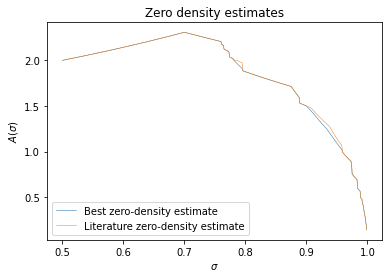
\includegraphics[width=0.5\linewidth]{chapter/zero_density_estimate_plot.png}
    \caption{The bounds in Table \ref{zero_density_estimates_table}, compared against the existing literature bounds on $\A(\sigma)$.}
    \label{fig:zero_density_estimate}
\end{figure}

For completeness, we list in Table \ref{zero_density_historical} some historical zero density theorems not already covered, which have now been superseded by more recent estimates.

\begin{table}[ht]
    \def\arraystretch{1.3}
    \centering
    \caption{Historical upper bounds on $\A(\sigma)$}
    \begin{tabular}{|c|c|c|}
    \hline
    $\A(\sigma)$ bound & Range & Reference\\
    \hline
    $4\sigma$ & $\frac{1}{2} \leq \sigma \le 1$ & Carlson (1921) \cite{carlson_uber_1921}\\
    \hline
    $2$ & $4/5 \leq \sigma \leq 1$ & Montgomery (1969) \cite{montgomery_1969} \\
    \hline
    $2$ & $0.8080 \leq \sigma \leq 1$ & Forti--Viola (1972) \cite{forti-viola} \\
    \hline
    $\frac{39}{115\sigma-75}$ & $55/67 \leq \sigma \leq 189/230$ & Huxley (1973) \cite{huxley_large_1973} \\
    \hline
    $2$ & $189/230 \leq \sigma \leq 78/89$ & Huxley (1973) \cite{huxley_large_1973} \\
    \hline
    $\frac{48}{37(2\sigma-1)}$ & $78/89 \leq \sigma \leq 61/74$ & Huxley (1973) \cite{huxley_large_1973} \\
    \hline
    $\frac{3}{2\sigma}$ & $37/42 \leq \sigma \leq 1$ & Huxley (1975) \cite{huxley_large_1975a}\\
    \hline
    $\frac{48}{37(2\sigma-1)}$ & $61/74 \leq \sigma \leq 37/42$ & Huxley (1975) \cite{huxley_large_1975a}\\
    \hline
    $2$ & $0.80119 \leq \sigma \leq 1$ & Huxley (1975) \cite{huxley_large_1975a}\\
    \hline
    $2$ & $4/5 \leq \sigma \leq 1$ & Huxley (1975) \cite{huxley_large_1975b}\\
    \hline
    $\frac{6}{5\sigma-1}$ & $67/87 \leq \sigma \leq 1$ & Ivi\'c (1979) \cite{ivic_note_1979} \\
    \hline
    $\frac{3}{34\sigma-25}$ & $28/37 \leq \sigma \leq 74/95$ & Ivi\'c (1979) \cite{ivic_note_1979} \\
    \hline
    $\frac{9}{7\sigma-1}$ & $74/95 \leq \sigma \leq 1$ & Ivi\'c (1979) \cite{ivic_note_1979} \\
    \hline
    $\frac{3}{2\sigma}$ & $4/5 \leq \sigma \leq 1$ & Ivi\'c (1979) \cite{ivic_note_1979} \\
    \hline
    $\frac{68}{98\sigma-47}$ & $115/166 \leq \sigma \leq 1$ & Ivi\'c (1979) \cite{ivic_note_1979} \\
    \hline
    $\frac{3}{2\sigma}$ & $3831/4791 \leq \sigma \leq 1$ & Ivi\'c (1980) \cite{ivic_exponent_pairs}  \\
    \hline
    $\frac{9}{7\sigma-1}$ & $41/53 \leq \sigma \leq 1$ & Ivi\'c (1980) \cite{ivic_exponent_pairs} \\
    \hline
    $\frac{6}{5\sigma-1}$ & $13/17 \leq \sigma \leq 1$ & Ivi\'c (1980) \cite{ivic_exponent_pairs} \\
    \hline
    $\frac{4}{2\sigma+1}$ & $17/18 \leq \sigma \leq 1$ & Ivi\'c (1980) \cite{ivic_exponent_pairs} \\
    \hline
    $\frac{24}{30\sigma-11}$ & $155/174 \leq \sigma \leq 17/18$ & Ivi\'c (1980) \cite{ivic_exponent_pairs} \\
    \hline
    $\frac{3}{7\sigma-4}$ & $3/4 \leq \sigma \leq 10/13$ & Ivi\'c (1983) \cite{ivic_topics_1983} \\
    \hline
    $\frac{9}{8\sigma-2}$ & $10/13 \leq \sigma \leq 1$ & Ivi\'c (1983) \cite{ivic_topics_1983} \\
    \hline
    $\frac{15}{22\sigma-10}$ & $10/13 \leq \sigma \leq 5/6$ & Ivi\'c (1984) \cite{ivic_zero_1984} \\
    \hline
    $\frac{3k}{(3k-2)\sigma+2-k}$ & $\frac{9k^2 -3k + 2}{12k^2 -5k + 2} \leq \sigma \leq 1$; $k \geq 2$ & Ivi\'c (1984) \cite{ivic_zero_1984} \\
    \hline
    $58.05 (1-\sigma)^{1/2}$ & $1/2 \leq \sigma \leq 1$ & Ford (2002) \cite{FordZeta} \\
    \hline
    $6.42 (1-\sigma)^{1/2}$ & $9/10 \leq \sigma \leq 1$ & Heath-Brown (2017) \cite{heathbrown_new_2017} \\
    \hline
    $3\sqrt{2}(1-\sigma)^{1/2}+18(1-\sigma)$ & $17/18 \leq \sigma \leq 1$ & Pintz (2023) \cite{pintz_density_2023}\\
    \hline
    \end{tabular}
    \label{zero_density_historical}
    \end{table}

{\bf TODO: enter this table into literature.py}

\section{Estimates for \texorpdfstring{$\sigma$}{sigma} very close to \texorpdfstring{$1/2$}{1/2} or \texorpdfstring{$1$}{1}}

Some additional estimates were established for $\sigma$ sufficiently close to $1/2$ or $1$.

Tur\'an \cite{turan} introduced the power sum method to establish
$$ A(1-\eta) \leq 2 + \eta^{0.14}$$
for $\eta$ small enough. Hal\'asz and Tur\'an \cite{halasz_distribution_1969} combined this method with the large values approach of Hal\'asz \cite{halasz_1968} to improve the bound to
\begin{equation}\label{a-eta}
  A(1-\eta) \leq C \eta^{1/2}
\end{equation}
with $C = 12,000$ for sufficiently small $\eta$.  See \cite{pintz_2022} for an alternate proof of these results.

The constant $C$ in \eqref{a-eta} was improved to $1304.37$ by Montgomery \cite[Theorem 12.3]{montgomery_topics_1971} (see also the remark after \cite[(11.97)]{ivic} for a correction), to $58.05$ by Ford \cite{FordZeta}, to $5.03$ by Heath-Brown \cite{heathbrown_new_2017} (the latter exploiting the resolution of the Vinogradov mean value conjecture \cite{bourgain_demeter_guth}), and to any $C > 3\sqrt{2}=4.242\dots$ in \cite{pintz_density_2023}. See also an explicit version at \cite{bellotti}.

``Log-free'' zero density estimates of the form
$$ N(1-\eta,T) \ll T^{B\eta}$$
for various $B$ were established starting with the work of Linnik \cite{linnik-1,linnik-2} and developed further in \cite{turan}, \cite{fogels}, \cite{bombieri_1974}, \cite{jutila_linnik}, \cite{gallagher_large_sieve}, \cite{graham_1978}, \cite{heath_brown_least_prime}. An explicit version of such estimates may be found in \cite{bellotti_2024}.

There is some work establishing bounds on $N(\sigma,T)$ for $\sigma$ very close to $1/2$, although these bounds do not make further improvements on $\A(\sigma)$.  Specifically, bounds of the form
$$ N(\sigma,T) \ll T^{1-\theta(2\sigma-1)} \log T$$
were established for $\theta=1/8$ by Selberg \cite{selberg_1946} (see \cite{simonic} for an explicit version), any $0 < \theta < 1/2$ by Jutila \cite{jutila-critical}, and any $0 < \theta < 4/7$ by Conrey (claimed in \cite{conrey_at_1989}, with a full proof given in \cite{baluyot_thesis}).  Note that the density hypothesis would follow if we could establish the claim for all $0 < \theta < 1$, but an improvement to Ingham's bound (Theorem \ref{thm:ingham_zero_density2}) would only occur once $\theta$ exceeded $2/3$.

\section{A heuristic for zero density estimates}

We can now state a rough heuristic as to what zero density estimates to expect from a given large value theorem:

\begin{heuristic}[Predicting a zero density estimate from a large value theorem]\label{lv-heuristic}\uses{lv-def, zero-def} Suppose that $1/2 \leq \sigma \leq 1$ and $\tau_0 \geq 1$ are such that one can prove $\LV(\sigma, \tau_0) \leq 3-3\sigma$ (i.e., the Montgomery conjecture holds here with a multiplicative loss of $3/2$).  Then in principle, one can hope to prove $\A(\sigma) \leq 3/\tau_0$.  Conversely, if one cannot prove $\LV(\sigma, \tau_0) \leq 3-3\sigma$, then the bound $\A(\sigma) \leq 3/\tau_0$ is likely out of reach.
\end{heuristic}

We justify this heuristic as follows, though we stress that the arguments that follow are not fully rigorous.  In the first part, we simply apply Corollary \ref{zero-large-cor2}.  In practice, the \eqref{lvo} is often more delicate than \eqref{lvoz} and ends up being the limiting factor for the bounds; furthermore, within \eqref{lvo}, it is the right endpoint $\tau=\tau_0$ of the range $2\tau_0/3 \leq \tau \leq \tau_0$ that ends up being the bottleneck; but this is precisely the claimed criterion $\LV(\sigma, \tau_0) \leq 3-3\sigma$.  We remark that in some cases (particularly for $\sigma$ close to one), the estimate \eqref{lvoz} ends up being more of the bottleneck than \eqref{lvo}, and so one should view $3/\tau_0$ here as a theoretical upper limit of methods rather than as a guaranteed bound.  (In particular, the need to also establish the bound $\LV_\zeta(\sigma, \frac{4}{3}\tau_0-\eps) < 4-4\sigma$ for $\eps>0$ small can sometimes be a more limiting factor.)

Conversely, suppose that
\begin{equation}\label{lst3}
    \LV(\sigma,\tau_0) > 3-3\sigma,
\end{equation}
but that one still wants to prove the bound $\A(\sigma) \leq 3/\tau_0$. Heuristically, Theorem \ref{zero-dens_implies_large} suggests that in order to do this, it is necessary to establish the bound $\LV_\zeta(\sigma,\tau)/\tau \leq \frac{3}{\tau_0}(1-\sigma)$ for all $\tau \geq 2$.  In particular, one should show that
$$ \LV_\zeta(\sigma,2\tau_0) \leq 6-6\sigma.$$
Let us consider the various options one has to do this.  There are ways to control zeta large values that do not apply to general large value estimates, such as moment estimates of the zeta function, exponent pairs, or control of $\beta$ and $\mu$.  However, at our current level of understanding, these techniques only control $\LV_\zeta(\sigma,\tau)$ for relatively small values of $\tau$, and in practice $2\tau_0$ is too large for these methods to apply; this exponent also tends to be too large for direct application of standard large value theorems to be useful.  Hence, the most viable option in practice is raising to a power (Lemma \ref{power-lemma}), using
$$ \LV_\zeta(\sigma,2\tau_0) \leq k \LV_\zeta(\sigma,2\tau_0/k)$$
for some natural number $k \geq 2$.  However, the most natural choice $k=2$ is blocked due to our hypothesis \eqref{lst3}, while in practice the $k \geq 3$ choice is blocked because of Lemma \ref{lv-lower}.  Hence it appears heuristically quite difficult to establish $\A(\sigma) \leq 3/\tau_0$ with current technology, in the event that \eqref{lst3} occurs.

In Table \ref{zero_density_heuristic} we list some examples in which the heuristic can actually be attained.  Note that this only covers some, but not all, of the best known zero density estimates in Table \ref{zero_density_estimates_table}, as there are often other bounds that need to be established that prevent the heuristic limit of $3/\tau_0$ from actually being attained; so one should take the heuristic with a certain grain of salt.

\begin{table}[ht]
    \def\arraystretch{1.3}
    \centering
    \caption{Examples of large value theorems, the values of $\tau_0$ and $\A(\sigma)$ they suggest, and rigorous zero density theorems that attain the predicted value for at least some ranges of $\sigma$.}
    \begin{tabular}{|c|c|c|c|}
    \hline
    Large value theorem & Predicted choice of $\tau_0$ & Predicted bound $\frac{3}{\tau_0}$ on $\A(\sigma)$ & Matching zero density theorem(s)\\
    \hline
    Theorem \ref{l2-mvt} & $2-\sigma$ & $\frac{3}{2-\sigma}$ & Theorem \ref{thm:ingham_zero_density2}\\
    \hline
    Theorem \ref{huxley-lv} & $3\sigma-1$ & $\frac{3}{3\sigma-1}$ & Theorem \ref{huxley-bound} \\
    \hline
    Theorem \ref{hb-opt} & $10\sigma-7$ & $\frac{3}{10\sigma-7}$ & Theorems \ref{hb-density}, \ref{hb-density2} \\
    \hline
    Theorem \ref{jutila-lvt}, $k=3$ & $\frac{7\sigma-1}{3}$ & $\frac{9}{7\sigma-1}$ & Theorems \ref{hb-density}, \ref{further_ivic_zero} \\
    \hline
    Lemma \ref{a-ivt-1}, $m=2$ & $\frac{4\sigma}{2}$ & $\frac{3}{2\sigma}$ & Corollary \ref{further_ivic_zero}, Theorem \ref{bourgain-zero-density-2000} \\
    \hline
    Lemma \ref{a-ivt-1}, $m=3$ & $\frac{7\sigma-1}{3}$ & $\frac{9}{7\sigma-1}$ & Theorems \ref{hb-density}, Corollary \ref{further_ivic_zero} \\
    \hline
    Lemma \ref{a-ivt-1}, $m=4$ & $\frac{10\sigma-2}{4}$ & $\frac{6}{5\sigma-1}$ & Corollary \ref{further_ivic_zero} \\
    \hline
    Lemma \ref{a-ivt} & $7\sigma-4$ & $\frac{3}{7\sigma-4}$ & Corollary \ref{ivic-near-34} \\
    \hline
    Lemma \ref{a-ivt} & $\frac{8\sigma-2}{3}$ & $\frac{9}{8\sigma-2}$ & Corollary \ref{ivic-near-34} \\
    \hline
    Theorem \ref{guth-maynard-lvt} & $\frac{5\sigma-3}{3}$ & $\frac{15}{5\sigma-3}$ & Theorem \ref{guth-maynard-density} \\
    \hline
    \end{tabular}
    \label{zero_density_heuristic}
    \end{table}

    One consequence of Heuristic \ref{lv-heuristic} is that, in the regimes where the heuristic is accurate, combining multiple large values theorems together are unlikely to achieve new zero density theorems that could not be accomplished with each large value theorem separately.

\chapter{Zero density energy theorems}\label{zero-density-energy-chapter}


\begin{definition}[Zero density exponents]\label{zeroe-def}  For $1/2 \leq \sigma \leq 1$ and $T>0$, let $N^*(\sigma,T)$ denote the additive energy $E_1(\Sigma)$ of the imaginary parts of the zeroes $\rho$ of the Riemann zeta function with $\mathrm{Re}(\rho) \geq \sigma$ and $|\mathrm{Im}(\rho)| \leq T$.  For fixed $1/2 \leq \sigma \leq 1$, the zero density exponent $A^*(\sigma) \in [-\infty,\infty)$ is the infimum of all exponents $\A^*$ for which one has
    $$ N^*(\sigma-\delta,T) \ll T^{A^* (1-\sigma)+o(1)}$$
for all unbounded $T$ and infinitesimal $\delta>0$.
\end{definition}

The exponent $\A^*(\sigma)$ is also essentially referred to as $B(\sigma)$ in \cite{heath_brown_consecutive_II} (though without the technical shift by $\delta$ in that reference).

\python{zero_density_energy_estimate}
\code{Zero_Density_Energy_Estimate}

\begin{lemma}[Basic properties of $\A^*$]\label{zeroe-basic}\uses{zeroe-def}
\begin{itemize}
\item[(i)] We have the trivial bounds
$$ 2\A(\sigma), 4\A(\sigma)-\frac{1}{1-\sigma} \leq \A^*(\sigma) \leq 3 \A(\sigma)$$
for any $1/2 \leq \sigma \leq 1$.
\item[(ii)] $\sigma \mapsto (1-\sigma) \A^*(\sigma)$ is non-increasing, with $\A^*(1/2)=6$ and $\A^*(1)=-\infty$.
\item[(iii)] If the Riemann hypothesis holds, then $\A^*(\sigma)=-\infty$ for all $1/2 < \sigma \leq 1$.
\end{itemize}
\end{lemma}

\python{zero_density_energy_estimate}
\code{add_trivial_zero_density_energy_estimates(hypotheses)}

\begin{proof}\uses{add-energy, zero-basic} The claim (i) follows from Lemma \ref{add-energy}(iv), and the remaining claims then follow from Lemma \ref{zero-basic}.\end{proof}

Upper bounds on $\A^*(\sigma)$ can be obtained from large value energy theorems via the following relation.

\begin{lemma}[Zero density energy from large values energy]\label{zeroe-from-large}\uses{lvze-def}  Let $1/2 < \sigma < 1$.  Then
$$ \A^*(\sigma)(1-\sigma) \leq \max\left( \sup_{\tau \geq 1} \LV^*_\zeta(\sigma,\tau)/\tau, \limsup_{\tau \to \infty} \LV^*(\sigma,\tau)/\tau \right).$$
\end{lemma}

\begin{proof}\uses{lve-basic,zero-from-large,add-energy, lve-asymp}
Write the right-hand side as $B$, then $B \geq 0$ (from Lemma \ref{lve-basic}(iii)) and we have
\begin{equation}\label{lvze-bound}
    \LV^*_\zeta(\sigma,\tau) \leq B \tau
\end{equation}
for all $\tau \geq 1$, and
\begin{equation}\label{lve-bound}
    \LV^*(\sigma,\tau) \leq (B+\eps) \tau
\end{equation}
whenever $\eps>0$ and $\tau$ is sufficiently large depending on $\eps$ (and $\sigma$).  It would suffice to show, for any $\eps>0$, that $N^*(\sigma,T) \ll T^{B+O(\eps)+o(1)}$ for unbounded $T$.

By dyadic decomposition, it suffices to show for unbounded $T$ that the additive energy of imaginary parts of zeroes in $[T,2T]$ is $\ll T^{B+O(\eps)+o(1)}$.  As in the proof of Lemma \ref{zero-from-large}, we can assume the imaginary parts are $1$-separated (here we take advantage of the triangle inequality in Lemma \ref{add-energy}(iii)).

Suppose that one has a zero $\sigma'+i t$ of this form.  Then by standard approximations to the zeta function, one has
$$ \sum_{n \leq T} \frac{1}{n^{\sigma'+it}} \ll T^{-1}.$$
Let $0 < \delta_1 < \eps$ be a small quantity (independent of $T$) to be chosen later, and let $0 < \delta_2 < \delta_1$ be sufficiently small depending on $\delta_1,\delta_2$.  By the triangle inequality, and refining the sequence $t'$ by a factor of at most $2$, we either have
$$ \bigg|\sum_{T^{\delta_1} \leq n \leq T} \frac{1}{n^{\sigma'+it}} \bigg| \gg T^{-\delta_2}$$
for all zeroes, or \eqref{td}
for all zeroes.

Suppose we are in the former (``Type I'') case, we can dyadically partition and conclude from the pigeonhole principle that
$$ \bigg| \sum_{n \in I} \frac{1}{n^{\sigma'+it}} \bigg| \gg T^{-\delta_2-o(1)}$$
for some interval $I$ in some $[N,2N]$ with $T^{\delta_1} \ll N \ll T$, with at most $O(\log T)$ different choices for $I$.  Performing a Fourier expansion of $n^{\sigma'}$ in $\log n$ and using the triangle inequality one can then deduce that
$$ \bigg| \sum_{n \in I} \frac{1}{n^{it'}} \bigg| \gg N^{\sigma'} T^{-\delta_2-o(1)}$$
for some $t' = t + O(T^{o(1)})$; refining the $t$ by a factor of $T^{o(1)}$ if necessary, we may assume that the $t'$ are $1$-separated and that the interval $I$ is independent of $t'$, and by passing to a subsequence we may assume that $T = N^{\tau+o(1)}$ for some $1 \leq \tau \leq 1/\delta_1$, then
$$ \bigg| \sum_{n \in I} \frac{1}{n^{it'}} \bigg| \gg N^{\sigma-\delta_2/\delta_1+o(1)}$$
for all $t'$.  If we let $\Sigma'$ denote the set of such $t'$, then by Definition \ref{lvze-def} we then have (for $\delta_2$ small enough) we have
$$ E_1(\Sigma') \ll N^{\LV^*_\zeta(\sigma,\tau) + \eps + o(1)} \ll T^{\LV^*_\zeta(\sigma,\tau)/\tau + \eps + o(1)}.$$
By Lemma \ref{add-energy}(i) this implies that the set $\Sigma$ of imaginary parts of zeroes under consideration also obeys the bound
$$ E_1(\Sigma) \ll T^{\LV^*_\zeta(\sigma,\tau)/\tau + \eps + o(1)}.$$
and the claim follows in this case from \eqref{lvze-bound}.

The Type II case similarly follows from \eqref{lve-bound} exactly as in the proof of Lemma \ref{zero-from-large}.
\end{proof}


\begin{corollary}\label{zeroe-large-cor-0}\uses{zeroe-def, lvze-def} Let $1/2 < \sigma < 1$ and $\tau_0 > 0$ be fixed.  Then
$$ \A^*(\sigma)(1-\sigma) \leq \max \left(\sup_{2 \leq \tau < \tau_0} \LV^*_\zeta(\sigma,\tau)/\tau, \sup_{\tau_0 \leq \tau \leq 2\tau_0} \LV^*(\sigma,\tau)/\tau\right)$$
\end{corollary}

\python{zero_density_energy_estimate}
\code{lver_to_energy_bound(LVER, LVER_zeta, sigma_interval)}

\begin{proof}  Repeat the proof of Corollary \ref{zero-large-cor-0}.
\end{proof}

\section{Known additive energy bounds}

\begin{proposition}[Additive energy under the Lindelof hypothesis]\label{zeroe-lindelof}\uses{zeroe-def}  Let $1/2 \leq \sigma \leq 1$ be fixed.  Then one has
    $$ \A^*(\sigma) \leq 8 - 4\sigma$$
    and $\A^*(\sigma) \leq 0$ if $\sigma > 3/4$.
\end{proposition}

\begin{proof} See \cite[Lemma 4]{heath_brown_consecutive_II}.
\end{proof}

\begin{theorem}[Heath-Brown's additive energy bound]\label{hb-energy-bound}\cite[Theorem 2]{heathbrown_zero_1979}\uses{zeroe-def}  Let $1/2 \leq \sigma \leq 1$ be fixed.  Then one can bound $A^*(\sigma)$ by
    \begin{align*}
        \frac{10-11\sigma}{(2-\sigma)(1-\sigma)} & \hbox{ for } 1/2 \leq \sigma \leq 2/3;\\
        \frac{18-19\sigma}{(4-2\sigma)(1-\sigma)} & \hbox{ for } 2/3 \leq \sigma \leq 3/4;\\
        \frac{12}{4\sigma-1} & \hbox{ for } 3/4 \leq \sigma \leq 1.
    \end{align*}
\end{theorem}

\literature
\code{add_zero_density_energy_heath_brown_1979()}
\derived
\code{prove_heath_brown_energy_estimate()}

\begin{proof}\uses{zeroe-large-cor-0, power-energy, hb-energy-simp, l2-mvt, hb-density, zeroe-basic, lvz-basic} We first suppose that $\sigma \leq 3/4$.  Here we apply Corollary \ref{zeroe-large-cor-0} with $\tau_0 = 2$.  The $\LV^*_\zeta$ supremum is now trivial, so it suffices to show that
\begin{equation}\label{second-claim}
        \rho^* \leq \max\left( \frac{10-11\sigma}{2-\sigma}, \frac{18-19\sigma}{4-2\sigma}\right) \tau
\end{equation}
whenever $(\sigma,\tau,\rho,\rho^*,s) \in \Energy$ with $2 \leq \tau \leq 3$.  Let $k$ be the first integer for which $1 \leq \tau/k \leq 3/2$, thus $k=2,3$ and also $\tau/(k+1) \leq 1$.  By Lemma \ref{power-energy}, there exist tuples
\begin{equation}\label{smak}
\left(\sigma, \frac{\tau}{k}, \rho', \frac{\rho^*}{k}, s'\right), \left(\sigma,\frac{\tau}{k+1}, \rho'', \frac{\rho^*}{k + 1}, s''\right)  \in \Energy.
\end{equation}
for some $\rho'$, $s'$, $\rho''$ and $s''$ satisfying
\[
\rho' \le \frac{\rho}{k},\qquad s' \le \frac{s}{k},\qquad \rho'' \le \frac{\rho}{k+1},\qquad s'' \le \frac{s}{k+1}.
\]
Applying Corollary \ref{hb-energy-simp} to the former tuple of \eqref{smak} and using $\rho' \le \rho/k$, we have
$$\frac{\rho^*}{k} \leq \max \left(\frac{3\rho}{k} + 1-2\sigma, \frac{\rho}{k} +4-4\sigma, \frac{5\rho}{2k} + \frac{3-4\sigma}{2}\right).$$
Write $\tau' := \tau/k$. Applying Lemma \ref{l2-mvt} to the first tuple of \eqref{smak} one has
$$\rho/k \leq \tau' + 1 - 2\sigma$$
while applying Lemma \ref{l2-mvt} to the second tuple of \eqref{smak} (recalling that $\tau/(k+1) \le 1$) gives
$$\rho/k = \frac{k+1}{k} \frac{\rho}{k+1} \leq \frac{k+1}{k} (2-2\sigma) \le 3-3\sigma$$
and thus
\begin{equation}\label{rho-k}
\rho/k \leq \min( \tau'+1-2\sigma, 3-3\sigma)
\end{equation}
and
\begin{equation*}
    \begin{split}
        \rho^*/k \leq \max(&3 \min(\tau'+1-2\sigma,3-3\sigma) + 1-2\sigma, \\
        &\min(\tau'+1-2\sigma,3-3\sigma) +4-4\sigma, \\
        &5\min(\tau'+1-2\sigma,3-3\sigma)/2 + (3-4\sigma)/2).
    \end{split}
\end{equation*}
A tedious calculation shows that for $1 \leq \tau' \leq 3/2$, we have
$$3 \min(\tau'+1-2\sigma,3-3\sigma) + 1-2\sigma \leq \frac{10-11\sigma}{2-\sigma} \tau',$$
$$ \min(\tau'+1-2\sigma,3-3\sigma) +4-4\sigma \leq \max\left( \frac{7-7\sigma}{2-\sigma}, 6-6\sigma\right)\tau'$$
and
$$5\min(\tau'+1-2\sigma,3-3\sigma)/2 + (3-4\sigma)/2 \leq \frac{18-19\sigma}{4-2\sigma} \tau'.$$
Since
$$\max\left( \frac{7-7\sigma}{2-\sigma}, 6-6\sigma\right) \leq \max\left(\frac{10-11\sigma}{2-\sigma}, \frac{18-19\sigma}{4-2\sigma}\right)$$
we obtain the claim.

Now suppose that $\sigma > 3/4$.  From Theorem \ref{hb-density} and Lemma \ref{zeroe-basic}(i) we are already done when $\sigma \geq 25/28$, so we may assume $\sigma < 25/28$.

Here we apply Corollary \ref{zeroe-large-cor-0} with $\tau_0 = 4\sigma-1$.  To control the $\LV^*_\zeta$ term, we need to establish
\begin{equation}\label{first-claim}
    \rho^* \leq \frac{12(1-\sigma)}{4\sigma-1} \tau
\end{equation}
whenever $(\sigma,\tau,\rho,\rho^*,s) \in \Energy_\zeta$ and $2 \leq \tau < 4\sigma-1$. We use Lemma \ref{lvz-basic}(ii) followed by Lemma \ref{hb-12} to give
$$ \rho^* \leq 3\rho \leq 3( 2\tau - 12 (\sigma-1/2) )$$
so the claim reduces to verifying
$$ 3( 2\tau - 12 (\sigma-1/2) ) \leq \frac{12(1-\sigma)}{4\sigma-1} \tau.$$
This holds with equality when $\tau = 4\sigma-1$, and the slope in $\tau$ is higher on the left-hand side for $\sigma>1/2$, so the claim \eqref{first-claim} follows.

It remains to establish
\begin{equation}\label{second-claim'}
    \rho^* \leq \frac{12(1-\sigma)}{4\sigma-1} \tau
\end{equation}
whenever $(\sigma,\tau,\rho,\rho^*,s) \in \Energy$ and $4\sigma-1 \leq \tau \leq 2(4\sigma-1)$.
Let $k$ be the first integer for which $(4\sigma-1)/2 \leq \tau/k \leq 3(4\sigma-1)/4$, thus $k=2,3$ and also $\tau/(k+1) \leq 4\sigma-1$.  By Lemma \ref{power-energy}, we have \eqref{smak}.
From Theorem \ref{huxley-lv} we have
$$\rho/k \leq \max(2-2\sigma, \tau' + 4 - 6\sigma)$$
and also
$$\rho/k = \frac{k+1}{k} \frac{\rho}{k+1} \leq \frac{k+1}{k} (2-2\sigma) \le 3-3\sigma$$
and hence
\begin{equation}\label{rhok} \rho/k \leq \min( \max(2-2\sigma, \tau' + 4 - 6\sigma), \tau'+4-6\sigma, 3-3\sigma).
\end{equation}
Among other things, this implies that $\rho/k \leq 1$.

From Theorem \ref{hbt} and $\rho' \le \rho/k$, we have
\begin{equation}\label{rhok-star}
\begin{split}
\rho^*/k \leq 1-2\sigma &+ \frac{1}{2}\max\left(\frac{\rho}{k}+1, \frac{2\rho}{k}, \frac{5\rho}{4k} + \frac{\tau'}{2}\right)\\
&+ \frac{1}{2}\max\left(\frac{\rho^*}{k}+1, \frac{4\rho}{k}, \frac{3\rho^*}{4k}+\frac{\rho}{k}+\frac{\tau'}{2}\right)
\end{split}
\end{equation}
where $\tau' := \tau/k$.  This expression is complicated, so we divide into cases.
First suppose that $\rho/k+1 \geq 5\rho/4k + \tau'/2$.  In this case the first maximum in the above expression is $\rho/k+1$, and we simplify to
$$ \rho^*/k \leq 3/2-2\sigma + \rho/2k + \max(\rho^*/k+1, 4\rho/k, 3\rho^*/4k+\rho/k+\tau'/2)/2,$$
which after solving for $\rho^*/k$ gives
$$ \rho^*/k \leq \max( \rho/2k + 4-4\sigma, 5\rho/2k + (3-4\sigma)/2, 8\rho/5k + 2\tau'/5 + (12-16\sigma)/5).$$
Inserting \eqref{rhok}, one can verify after a tedious analysis (using the hypothesis $3/4 \leq \sigma < 25/28$) that
\begin{equation}\label{rhost}
    \rho^*/k \leq \frac{12(1-\sigma)}{4\sigma-1} \tau'
\end{equation}
as required.

It remains to treat the case where $\rho/k+1 > 5\rho/4k + \tau'/2$.  Using \eqref{rhok} one can check that this forces
\begin{equation}\label{4s}
    4\sigma-2 \leq \tau' \leq \frac{3}{4}(4\sigma-1),
\end{equation}
so that \eqref{rhok} now becomes
\begin{equation}\label{rhok-simp}
\rho/k \leq 3-3\sigma.
\end{equation}
The bound \eqref{rhok-star} becomes
$$\rho^*/k \leq 1-2\sigma + (5\rho/4k+\tau'/2)/2 + \max(\rho^*/k+1, 4\rho/k, 3\rho^*/4k+\rho/k+\tau'/2)/2$$
which simplifies to
$$ \rho^*/k \leq \max( 5\rho/4k + \tau'/2 + 3-4\sigma, 21\rho/8k + \tau'/4 + 1-2\sigma, 9\rho/5k + 4\tau'/5 + (8 - 16\sigma)/5).$$
Inserting \eqref{rhok-simp} and \eqref{4s}, one can eventually show (again using the hypothesis $3/4 \leq \sigma < 25/28$) that
\eqref{rhost} holds as required.
\end{proof}

We found the following estimates with the use of computer-aided proof discovery, which improve on Theorem \ref{hb-energy-bound} in various ranges of $\sigma$. First, by using Theorem \ref{hbt} in place of Corollary \ref{hb-energy-simp} in the proof of the previous theorem, it is possible to obtain an improved additive energy estimate for $\sigma \ge 3/4$. A human-readable proof is contained in the following theorem.

\begin{theorem}\label{imp-hb-energy-bound}
For $3/4 \le \sigma \le 5/6$ one has
\[
\A^*(\sigma) \le \max\left(\frac{18 - 19\sigma}{2(3\sigma - 1)(1-\sigma)}, \frac{4(10 - 9\sigma)}{5(4\sigma - 1)(1 - \sigma)}\right).
\]
\end{theorem}

\derived
\code{prove_improved_heath_brown_energy_estimate()}

\begin{proof}
Throughout assume that $3/4 \le \sigma \le 5/6$. Choose
\[
\tau_0 = 8\sigma - 4.
\]
We will show that
\begin{equation}\label{imphb-lver-ineq}
\rho^* \le \begin{cases}
\dfrac{18 - 19\sigma}{2(3\sigma - 1)}\tau,&3/4 \le \sigma < 4/5\\
\dfrac{7(1 - \sigma)}{3\sigma - 1}\tau,&4/5 \le \sigma \le 5/6,
\end{cases}
\end{equation}
for all $(\sigma, \tau, \rho, \rho^*, s) \in \Energy$ for which $\tau_0 \le \tau \le 2\tau_0$, and that
\begin{equation}\label{imphb-zlver-ineq}
\rho^* \le \begin{cases}
\dfrac{45 - 46\sigma}{4(4\sigma - 1)}\tau,&3/4 \le \sigma < 65/86,\\
\dfrac{4(10 - 9\sigma)}{5(4\sigma - 1)}\tau,&65/86 \le \sigma \le 5/6.
\end{cases}
\end{equation}
for all $(\sigma, \tau, \rho, \rho^*, s) \in \Energy_\zeta$ such that $2 \le \tau \le \tau_0$. The desired result then follows from Corollary \ref{zeroe-large-cor-0} and computing the piecewise maximum of \eqref{imphb-lver-ineq} and \eqref{imphb-zlver-ineq}.

First, consider \eqref{imphb-zlver-ineq}. Suppose that $(\sigma, \tau, \rho, \rho^*, s)\in \Energy_\zeta$ with $3/4 \le \sigma \le 5/6$ and $2 \le \tau \le \tau_0$. Then, from Theorem \ref{hb-12},
\begin{equation}\label{hb-lv-rho-form}
\rho \le 2\tau - 12(\sigma - 1/2).
\end{equation}
Furthermore, by Theorem \ref{huxley-lv} and Lemma \ref{power-lemma} with $k = 2$, one has $\rho \le 2\max(2 - 2\sigma, 4 - 6\sigma + \tau/2)$. However since $\tau \le \tau_0 = 8\sigma - 4$, this simplifies to
\begin{equation}
\label{huxley-lv-rho-form2}
\rho \le 4 - 4\sigma.
\end{equation}
Since $\sigma \ge 3/4$, this also implies that $\rho \le 1$. For future reference we also note that
\begin{equation}\label{zlver:tau-gradient-1}
1 < \frac{45 - 46\sigma}{4(4\sigma - 1)} < 2,\qquad (3/4 \le \sigma \le 65/86),
\end{equation}
\begin{equation}\label{zlver:tau-gradient-2}
\frac{6}{7} \le \frac{4(10 - 9\sigma)}{5(4\sigma - 1)} < 2,\qquad (65/86 \le \sigma \le 5/6).
\end{equation}
By Theorem \ref{hbt}, one has
\[
\rho^* \leq 1-2\sigma + \frac{1}{2}\max(\rho+1, 2\rho, \frac{5}{4}\rho+\frac{\tau}{2}) + \frac{1}{2}\max(\rho^*+1, 4\rho, \frac{3}{4}\rho^*+\rho+\frac{\tau}{2})
\]
Since $\rho \le 1$, one has $\rho + 1 \ge 2\rho$. Thus the middle term in the first maximum may be omitted, and we are left with two cases to consider.

\textbf{Case 1:} If $\rho + 1 \ge 5\rho/4 + \tau/2$ then
\[
\rho^* \le 1 -2\sigma + \frac{\rho + 1}{2} + \frac{1}{2}\max(\rho^* + 1, 4\rho, \frac{3}{4}\rho^*+\rho +\frac{\tau}{2}).
\]
Solving for $\rho^*$ gives
\[
\rho^* \le \max(4 - 4\sigma + \rho, \frac{3}{2} - 2\sigma + \frac{5}{2}\rho, \frac{2}{5}(6 - 8\sigma + \tau + 4\rho)).
\]
Applying \eqref{huxley-lv-rho-form2} to each term,
\[
\rho^* \le M_1 := \max(8 - 8\sigma, \frac{23}{2} - 12\sigma, \frac{2}{5}(22 - 24\sigma + \tau)).
\]
For $3/4 \le \sigma \le 5/6$ and $\tau \ge 2$, one has
\[
M_1 \le \frac{45 - 46\sigma}{4(4\sigma - 1)}\tau
\]
since by \eqref{zlver:tau-gradient-1}, each term in $M_1$ increases slower in $\tau$ than the RHS, and the inequality holds at $\tau = 2$. Similarly, one can verify that
\[
M_1 \le \frac{4(10 - 9\sigma)}{5(4\sigma - 1)}\tau
\]
for $65/86 \le \sigma \le 5/6$ and $\tau \ge 2$ (with some room to spare).

\textbf{Case 2:} If $\rho + 1 < 5\rho/4 + \tau/2$, then
\[
\rho^* \le 1 - 2\sigma + \frac{5}{8}\rho + \frac{\tau}{4} + \frac{1}{2}\max(\rho^* + 1, 4\rho, \frac{3}{4}\rho^*+\rho +\frac{\tau}{2})
\]
Solving for $\rho$ gives
\[
\rho^* \le \max(3 - 4\sigma + \frac{\tau}{2} + \frac{5}{4}\rho, 1 - 2\sigma + \frac{\tau}{4} + \frac{21}{8}\rho, \frac{8 - 16\sigma + 4\tau + 9\rho}{5})
\]
If $\tau \ge 4\sigma - 1$, then apply \eqref{huxley-lv-rho-form2} termwise to get
\[
\rho^* \le M_2 := \max(8 - 9\sigma + \frac{\tau}{2}, \frac{23}{2} - \frac{25}{2} + \frac{\tau}{4}, \frac{4}{5}(11 - 13 \sigma + \tau)).
\]
For $3/4 \le \sigma \le 65/86$ and $\tau \ge 4\sigma - 1$ one has
\[
M_2 \le \frac{45 - 46\sigma}{4(4\sigma - 1)}\tau
\]
since by \eqref{zlver:tau-gradient-2} each term in $M_2$ is growing slower in $\tau$ than the RHS, and at $\tau = 4\sigma - 1$ we have equality. Similarly, one may verify that $M_2 \le 4(10 - 9\sigma)/(5(4\sigma - 1))\tau$ for $65/86 \le \sigma \le 5/6$ and $\tau \ge 4\sigma - 1$.

On the other hand if $\tau < 4\sigma - 1$ then we apply \eqref{hb-lv-rho-form} termwise to get
\[
\rho^* \le M_3 := \max(\frac{21}{2} - 19\sigma + 3\tau, \frac{67 -134\sigma + 22\tau}{4}, \frac{2}{5}(31 - 62\sigma + 11\tau)).
\]
Similarly to before, if $3/4 \le \sigma \le 65/86$ and $\tau < 4\sigma - 1$ then
\[
M_3 < \frac{45 - 46\sigma}{4(4\sigma - 1)}\tau
\]
since each term in $M_3$ is growing faster in $\tau$ than the RHS, and at $\tau = 4\sigma - 1$ one has equality. Similarly, one may verify that $M_3 \le 4(10 - 9\sigma)/(5(4\sigma - 1))\tau$ for $65/86 \le \sigma \le 5/6$ and $\tau < 4\sigma - 1$.

Thus we have shown that if $(\sigma, \tau, \rho, \rho^*, s) \in \Energy_\zeta$ with $3/4 \le \sigma \le 5/6$ and $2 \le \tau \le 8\sigma - 4$, then
\[
\rho^*/\tau \le \min\left(\frac{45 - 46\sigma}{4(4\sigma - 1)}, \frac{4(10 - 9\sigma)}{5(4\sigma - 1)}\right).
\]

Now consider \eqref{imphb-lver-ineq}. Suppose that $\tau_0 \le \tau \le 2\tau_0$ and $(\sigma, \tau, \rho, \rho^*, s) \in \Energy$. Note that the interval $[\tau_0, 2\tau_0]$ is covered by intervals $I_k := [(4\sigma - 2)k, (4\sigma - 2)(k + 1)]$ with $k = 2, 3$. Suppose that $\tau \in I_k$. Then, by Theorem \ref{huxley-lv} and $\tau \ge (4\sigma - 2)k$ one has
\[
\rho/k \le \max(2 - 2\sigma, 4 - 6\sigma + \tau/k) = 4 - 6\sigma + \tau/k.
\]
Also, from Theorem \ref{huxley-lv} and $\tau \le (4\sigma - 2)(k + 1)$ one has
\[
\rho/(k + 1) \le \max(2 - 2\sigma, 4 - 6\sigma + \tau/(k + 1)) \le 2 - 2\sigma.
\]
In summary,
\begin{equation}\label{ze-ihb-rho-bound-k}
\rho/k \le \min((2 - 2\sigma)\frac{k + 1}{k}, 4 - 6\sigma + \frac{\tau}{k}).
\end{equation}
In particular, this implies that $\rho/k \le 1$ since $\sigma \ge 3/4$ implies $3 - 3\sigma < 1$.

We also note for future use that
\begin{equation}\label{ze-ihb-bound-tau-factor}
1 \le \frac{18 - 19\sigma}{6\sigma - 2} \le \frac{3}{2}.
\end{equation}
Next, by Lemma \ref{power-energy},
\[
(\sigma, \tau', \rho', \rho^*/k, s') \in \Energy
\]
for $\tau' := \tau/k$ and some $\rho' \le \rho/k$ and $s' \le s/k$.

Applying Lemma \ref{hbt} to this tuple, then apply $\rho' \le \rho/k$:
\[
\rho^*/k \leq 1-2\sigma + \frac{1}{2}\max(\frac{\rho}{k}+1, \frac{2\rho}{k}, \frac{5\rho}{4k} + \frac{\tau'}{2}) + \frac{1}{2}\max(\frac{\rho^*}{k}+1, \frac{4\rho}{k}, \frac{3}{4}\frac{\rho^*}{k} +\frac{\rho}{k}+\frac{\tau'}{2})
\]
Since $\rho/k \le 1$ there are only two cases to consider:

\textbf{Case 1:} $\rho/k + 1 \ge 5\rho/(4k) + \tau'/2$ then
\[
\frac{\rho^*}{k} \le \frac{3}{2} - 2\sigma + \frac{\rho}{2k} + \frac{1}{2}\max(\frac{\rho^*}{k}+1, \frac{4\rho}{k}, \frac{3}{4}\frac{\rho^*}{k} +\frac{\rho}{k}+\frac{\tau'}{2})
\]
Solving for $\rho^*/k$, we get
\[
\rho^*/k \le \max(4(1 - \sigma) + \frac{\rho}{k}, \frac{(3 - 4\sigma) + 5\rho/k}{2}, \frac{2}{5}((6 - 8\sigma) + \tau' + \frac{4\rho}{k}))
\]
If $4\sigma - 2 + 2(1 - \sigma)/k \le \tau' \le (4\sigma - 2)(k + 1)/k$ then by applying $\rho/k \le (2 - 2\sigma)(k + 1)/k$ from \eqref{ze-ihb-rho-bound-k}, one has
\[
\rho^*/k \le \max((6 + \frac{2}{k})(1 - \sigma), \frac{13}{2} - 7\sigma + \frac{5}{k} (1 - \sigma), \frac{2}{5}(14 - 16\sigma + \tau' + \frac{8}{k}(1 - \sigma)))
\]
However for $3/4 \le \sigma \le 4/5$, $k \ge 2$ and $\tau' \ge 4\sigma - 2 + 2(1 - \sigma)/k$ one has
\begin{align*}
\frac{18 - 19\sigma}{6\sigma - 2}\tau' - (6 + \frac{2}{k})(1 - \sigma) &\ge \frac{18 - 19\sigma}{6\sigma - 2}(4\sigma - 2 + \frac{2}{k}(1 - \sigma)) - (6 + \frac{2}{k})(1 - \sigma) \\
&= \frac{(4 - 5\sigma) ((4\sigma - 3)k - 5\sigma + 5)}{k(3\sigma - 1)} \ge 0,
\end{align*}
\begin{align*}
&\frac{18 - 19\sigma}{6\sigma - 2}\tau' - \left(\frac{13}{2} - 7\sigma + \frac{5}{k} (1 - \sigma)\right) \\
&\qquad\ge \frac{18 - 19\sigma}{6\sigma - 2}(4\sigma - 2 + \frac{2}{k}(1 - \sigma)) - \left(\frac{13}{2} - 7\sigma + \frac{5}{k} (1 - \sigma)\right) \\
&\qquad= \frac{(k - 2) (34\sigma - 23) (1 - \sigma)}{2 k (3\sigma - 1)} \ge 0,
\end{align*}
\begin{align*}
&\frac{18 - 19\sigma}{6\sigma - 2}\tau' - \frac{2}{5}(14 - 16\sigma + \tau' + \frac{8}{k}(1 - \sigma)) \\
&\qquad\ge \left(\frac{18 - 19\sigma}{6\sigma - 2} - \frac{2}{5}\right)(4\sigma - 2 + \frac{2}{k}(1 - \sigma)) - \frac{2}{5}(14 - 16\sigma + \frac{8}{k}(1 - \sigma))\\
&\qquad= \begin{cases}
(22 - 27\sigma)/10,&k = 2,\\
(88 - 272\sigma + 199\sigma^2)/(15(1 - 3\sigma)),&k=3,
\end{cases}\\
&\qquad\ge 0.
\end{align*}
Therefore
\begin{equation}\label{ze-ihb-rhok-targetbound}
\rho^*/k \le \frac{18 - 19\sigma}{6\sigma - 2}\tau'
\end{equation}
in this case.

On the other hand, if $4\sigma - 2 \le \tau' \le 4\sigma - 2 + 2(1 - \sigma)/k$ then applying $\rho/k \le 4 - 6\sigma + \tau'$ one has
\[
\rho^*/k \le \max(8 -10\sigma + \tau',\frac{23 - 34\sigma + 5\tau'}{2}, \frac{2}{5}(22 - 32\sigma +  5\tau'))
\]
Similarly to before, for $3/4 \le \sigma \le 4/5$ and $4\sigma - 2 \le \tau' \le 4\sigma - 2 + 2(1 - \sigma)/k$ one has (in view of \eqref{ze-ihb-bound-tau-factor})
\begin{align*}
\frac{18 - 19\sigma}{6\sigma - 2}\tau' - (8 - 10\sigma + \tau') &\ge \left(\frac{18 - 19\sigma}{6\sigma - 2} - 1\right)(4\sigma - 2) - (8 - 10\sigma) \\
&= \frac{20}{3}\frac{(\sigma - 3/4) (4/5 - \sigma)}{\sigma - 1/3} \ge 0,
\end{align*}
\begin{align*}
\frac{18 - 19\sigma}{6\sigma - 2}\tau' - \frac{23 - 34\sigma + 5\tau'}{2} &\ge \left(\frac{18 - 19\sigma}{6\sigma - 2} - \frac{5}{2}\right)(4\sigma - 2 + \frac{2}{k}(1 - \sigma)) - \frac{23 - 34\sigma}{2}\\
&= \frac{(k - 2)(34\sigma - 23)(1 - \sigma)}{2k(3\sigma - 1)} \ge 0,
\end{align*}
\begin{align*}
\frac{18 - 19\sigma}{6\sigma - 2}\tau' - \frac{2}{5}(22 - 32\sigma +  5\tau') &\ge \left(\frac{18 - 19\sigma}{6\sigma - 2} - 2\right)(4\sigma - 2 + \frac{2}{k}(1 - \sigma)) - \frac{2}{5}(22 - 32\sigma)\\
&= \begin{cases}
(22 - 27\sigma)/10,&k = 2,\\
(88 - 272\sigma + 199\sigma^2)/(15(1 - 3\sigma)),&k=3,
\end{cases}\\
&\ge 0.
\end{align*}
Therefore, \eqref{ze-ihb-rhok-targetbound} holds in this case too.

\textbf{Case 2:} $\rho/k + 1 < 5\rho/(4k) + \tau'/2$ then
\[
\rho^*/k \leq 1-2\sigma + \frac{5\rho}{8k} + \frac{\tau'}{4} + \frac{1}{2}\max(\frac{\rho^*}{k}+1, \frac{4\rho}{k}, \frac{3}{4}\frac{\rho^*}{k} + \frac{\rho}{k}+\frac{\tau'}{2})
\]
Solving for $\rho^*/k$ gives
\[
\rho^*/k \le \max(3 - 4\sigma + \frac{\tau'}{2} + \frac{5}{4}\frac{\rho}{k}, 1 - 2\sigma + \frac{\tau'}{4} + \frac{21}{8}\frac{\rho}{k}, \frac{1}{5}(8 - 16\sigma + 4\tau' + 9\frac{\rho}{k}))
\]
Proceeding as before, if $4\sigma - 2 + 2(1 - \sigma)/k \le \tau' \le (4\sigma - 2)(k + 1)/k$ then by applying $\rho/k \le (2 - 2\sigma)(k + 1)/k$ from \eqref{ze-ihb-rho-bound-k}, one has
\begin{align*}
\rho^*/k \le \max(&\frac{11 - 13\sigma + \tau' + 5(1 - \sigma)/k}{2}, \frac{25 - 29\sigma + \tau' + 21(1-\sigma)/k}{4},\\
&\qquad\frac{2}{5}(13 - 17 \sigma + 2\tau' + 9 (1 - \sigma)/k))
\end{align*}
Via a similar argument to before, using \eqref{ze-ihb-bound-tau-factor} and $\tau' \ge 4\sigma - 2 + 2(1 - \sigma)/k$ one eventually obtains, for $3/4 \le \sigma \le 4/5$,
\[
\frac{18 - 19\sigma}{6\sigma - 2}\tau' - \frac{11 - 13\sigma + \tau' + 5(1 - \sigma)/k}{2} \ge \begin{cases}
(11 - 13\sigma)/4,&k = 2\\
(44\sigma^2 - 60\sigma + 19)/(3 - 9\sigma),&k=3
\end{cases}\ge 0,
\]
\[
\frac{18 - 19\sigma}{6\sigma - 2}\tau' - \frac{25 - 29\sigma + \tau' + 21(1-\sigma)/k}{4} \ge \frac{(1 - \sigma) (95 - 49 k - (145 - 77 k)\sigma)}{4 k (3\sigma - 1)} \ge 0,
\]
\[
\frac{18 - 19\sigma}{6\sigma - 2}\tau' - \frac{2}{5}(13 - 17 \sigma + 2\tau' + 9(1 - \sigma)/k)) = \begin{cases}
(28 - 33\sigma)/10,&k = 2\\
(47\sigma^2 - 64\sigma + 20)/(3 - 9\sigma)&k=3
\end{cases}\ge 0.
\]
Thus also
\[
\rho^*/k \le \frac{18 - 19\sigma}{6\sigma - 2}\tau'
\]
in this case.

Similarly, if $(4\sigma - 2) \le \tau' \le 4\sigma - 2 + 2(1 - \sigma)/k$ then using $\rho/k \le 4 - 6\sigma + \tau'$ from \eqref{ze-ihb-rho-bound-k} one has
\[
\rho^*/k \le \max(8 - \frac{23\sigma}{2} + \frac{7\tau'}{4}, \frac{23}{2} - \frac{71\sigma}{4} + \frac{23\tau'}{8}, \frac{44 - 70\sigma + 13\tau'}{5})
\]
Via a similar argument as before, using \eqref{ze-ihb-bound-tau-factor} and $\tau' \le 4\sigma - 2 + 2(1 - \sigma)/k$ one ultimately obtains, for $3/4 \le \sigma \le 4/5$,
\[
\frac{18 - 19\sigma}{6\sigma - 2}\tau' - (8 - \frac{23\sigma}{2} + \frac{7\tau'}{4}) \ge \begin{cases}
(11 - 13 \sigma)/4,&k = 2\\
(44\sigma^2 - 60\sigma + 19)/(3 - 9\sigma),&k = 3
\end{cases} > 0,
\]
\[
\frac{18 - 19\sigma}{6\sigma - 2}\tau' - (\frac{23}{2} - \frac{71\sigma}{4} + \frac{23\tau'}{8}) \ge \frac{(1 - \sigma) (95 - 49 k - (145 - 77 k)\sigma)}{4 k (3\sigma - 1)} > 0,
\]
\[
\frac{18 - 19\sigma}{6\sigma - 2}\tau' - \frac{44 - 70\sigma + 13\tau'}{5} \ge \begin{cases}
(28 - 33\sigma)/10,&k = 2\\
(47\sigma^2 - 64\sigma + 20)/(3 - 9\sigma),&k=3
\end{cases} > 0.
\]
Combining all the cases, we have shown that for $3/4 \le \sigma \le 4/5$ and $\tau_0 \le \tau \le 2\tau_0$ one has
\[
\rho^*/k \le \frac{18 - 19\sigma}{6\sigma - 2}\tau'
\]
from which the desired result follows.

The case for $4/5 \le \sigma \le 5/6$ may be treated similarly. Here one may verify that
\[
\max((6 + \frac{2}{k})(1 - \sigma), \frac{13}{2} - 7\sigma + \frac{5}{k} (1 - \sigma), \frac{2}{5}(14 - 16\sigma + \tau' + \frac{8}{k}(1 - \sigma))) \le \frac{7(1 - \sigma)}{3\sigma - 1}\tau',
\]
\begin{align*}
&\max(\frac{11 - 13\sigma + \tau' + 5(1 - \sigma)/k}{2}, \frac{25 - 29\sigma + \tau' + 21(1-\sigma)/k}{4},\\
&\qquad\qquad\frac{2}{5}(13 - 17 \sigma + 2\tau' + 9 (1 - \sigma)/k)) \le \frac{7(1 - \sigma)}{3\sigma - 1}\tau'
\end{align*}
for $4\sigma - 2 + 2(1 - \sigma)/k \le \tau' \le (4\sigma - 2)(k + 1)/k$, and that
\[
\max(8 -10\sigma + \tau',\frac{23 - 34\sigma + 5\tau'}{2}, \frac{2}{5}(22 - 32\sigma +  5\tau')) \le \frac{7(1 - \sigma)}{3\sigma - 1}\tau',
\]
\[
\max(8 - \frac{23\sigma}{2} + \frac{7\tau'}{4}, \frac{23}{2} - \frac{71\sigma}{4} + \frac{23\tau'}{8}, \frac{44 - 70\sigma + 13\tau'}{5}) \le \frac{7(1 - \sigma)}{3\sigma - 1}\tau'
\]
for $4\sigma - 2 \le \tau' \le 4\sigma - 2 + 2(1 - \sigma)/k$. The treatment is analogous to before, so we omit the proof.
\end{proof}

Using Theorem \ref{guth-maynard-lvt}, it is possible to obtain improved energy estimates near $\sigma = 3/4$, which are given by the next two theorems.

\begin{theorem}\label{imp-energy-bound2}
For $7/10 \le \sigma \le 3/4$, one has
\[
\A^*(\sigma) \le \max\left(\frac{5(18 - 19\sigma)}{2(5\sigma + 3)(1 - \sigma)}, \frac{2(45 - 44\sigma)}{(2\sigma + 15)(1
- \sigma)}\right).
\]
\end{theorem}

\derived
\code{prove_zero_density_energy_2()}

\begin{proof}

Throughout assume $7/10 \le \sigma \le 3/4$ and take $\tau_0 = 2$ in Corollary \ref{zeroe-large-cor-0}. It suffices to show that if $(\sigma, \tau, \rho, \rho^*, s) \in \Energy$ with $2 \le \tau \le 4$, then either
\begin{equation}
\rho^* \le \frac{5(18 - 19\sigma)}{2(5\sigma + 3)}\tau
\end{equation}
or
\begin{equation}
\rho^* \le \frac{2(45 - 44\sigma)}{2\sigma + 15}\tau.
\end{equation}
Note for future reference the crude bounds
\begin{equation}\label{ze-bound2-tau-factor-bounds}
1 < \frac{5(18 - 19\sigma)}{2(5\sigma + 3)} < 2,\qquad 1 < \frac{2(45 - 44\sigma)}{2\sigma + 15} < \frac{7}{4}.
\end{equation}
Let
\[
k := \begin{cases}
2,& 2 \le \tau < 3,\\
3,& 3 \le \tau \le 4,
\end{cases},\qquad \tau' := \tau/k.
\]
Via Theorem \ref{l2-mvt} and Lemma \ref{power-lemma}, one has
\begin{equation}\label{ze-bound2-rho1}
\rho/k \le \max(2 - 2\sigma, 1 - 2\sigma + \tau')
\end{equation}
and via Theorem \ref{guth-maynard-lvt} and Lemma \ref{power-lemma}, one has
\[
\rho/k\le \max(2 - 2\sigma, 18/5 - 4\sigma, 12/5 - 4\sigma + \tau').
\]
Since $\sigma \le 4/5$, we may drop the first term, i.e.
\begin{equation}\label{ze-bound2-rho2}
\rho/k \le \max(18/5 - 4\sigma, 12/5 - 4\sigma + \tau').
\end{equation}
Combining \eqref{ze-bound2-rho1} and \eqref{ze-bound2-rho2},
\begin{equation}\label{ze-bound2-rhok-bound}
\rho/k \le \begin{cases}
1 - 2\sigma + \tau',&1 \le \tau' \le 13/5 - 2\sigma,\\
18/5 - 4\sigma,& 13/5 - 2\sigma \le \tau' \le 6/5,\\
12/5 - 4\sigma + \tau',& 6/5 \le \tau' \le 2(\sigma - 1/5) + 2(1 - \sigma)/k,\\
(2 - 2\sigma)(k + 1)/k,& 2(\sigma - 1/5) + 2(1 - \sigma)/k \le \tau' \le 1 + 1/k.
\end{cases}
\end{equation}
One can verify that all intervals are proper for $7/10 \le \sigma \le 3/4$ and $k = 2,3$.

Since $(\sigma, \tau, \rho, \rho^*, s) \in \Energy$, by Lemma \ref{power-energy} one has $(\sigma, \tau', \rho', \rho^*/k, s') \in \Energy$ for some $\rho' \le \rho/k$ and $s'\le s/k$. Applying Theorem \eqref{hbt}to the first tuple followed by $\rho' \le \rho/k$, and noting that $\rho/k + 1 \ge 2\rho/k$ since $\rho/k \le 1$ by \eqref{ze-bound2-rhok-bound}, one obtains
\begin{equation}\label{ze-bound2-rhostar-boundk}
\frac{\rho^*}{k} \le 1-2\sigma + \frac{1}{2}\max\left(\frac{\rho}{k}+1, \frac{5\rho}{4k} + \frac{\tau'}{2}\right) + \frac{1}{2}\max\left(\frac{\rho^*}{k}+1, \frac{4\rho}{k}, \frac{3\rho^*}{4k} +\frac{\rho}{k}+\frac{\tau'}{2}\right).
\end{equation}
First, suppose that $\rho/k  + 1 < 5\rho/(4k) + \tau'/2$ so that
\[
\frac{\rho^*}{k} \leq 1-2\sigma + \frac{5\rho}{8k} + \frac{\tau'}{4} + \frac{1}{2}\max\left(\frac{\rho^*}{k}+1, \frac{4\rho}{k}, \frac{3}{4}\frac{\rho^*}{k} + \frac{\rho}{k}+\frac{\tau'}{2}\right).
\]
Solving for $\rho^*/k$ gives
\[
\frac{\rho^*}{k} \le \max\left(3 - 4\sigma + \frac{\tau'}{2} + \frac{5}{4}\frac{\rho}{k}, 1 - 2\sigma + \frac{\tau'}{4} + \frac{21}{8}\frac{\rho}{k}, \frac{1}{5}(8 - 16\sigma + 4\tau' + 9\frac{\rho}{k})\right).
\]
One may verify that the RHS is bounded by
\[
\frac{5(18 - 19\sigma)}{2(5\sigma + 3)}\tau'
\]
by substituting each case of \eqref{ze-bound2-rhok-bound}. This involves the tedious verification of the following four inequalities:
\begin{equation}\label{ze-bound2-rho-case1-1}
\max\left(\frac{17}{4} - \frac{13}{2}\sigma + \frac{7}{4}\tau', \frac{29}{8} - \frac{29}{4}\sigma + \frac{23}{8}\tau', \frac{17}{5} - \frac{34}{5}\sigma + \frac{13}{5}\tau'\right) \le \frac{5(18 - 19\sigma)}{2(5\sigma + 3)}\tau'
\end{equation}
for $1 \le \tau' \le 13/5 - 2\sigma$;
\[
\max\left(\frac{15}{2} - 9\sigma + \frac{\tau'}{2}, \frac{209}{20} - \frac{25}{2}\sigma + \frac{\tau'}{4}, \frac{202}{25} - \frac{52}{5}\sigma + \frac{4}{5}\tau'\right) \le \frac{5(18 - 19\sigma)}{2(5\sigma + 3)}\tau'
\]
for $13/5 - 2\sigma \le \tau' \le 6/5$;
\[
\max\left(6 - 9\sigma + \frac{7}{4}\tau', \frac{73}{10} - \frac{25}{2}\sigma + \frac{23}{8}\tau', \frac{148}{25} - \frac{52}{5}\sigma + \frac{13}{5}\tau'\right) \le \frac{5(18 - 19\sigma)}{2(5\sigma + 3)}\tau'
\]
for $k = 2, 3$ and $6/5 \le \tau' \le 2(\sigma - 1/5) + 2(1-\sigma)/k$;
\begin{equation*}
\begin{split}
\max(&3 - 4\sigma + \frac{\tau'}{2} + \frac{5(2 - 2\sigma)}{4}\frac{k + 1}{k}, 1 - 2\sigma + \frac{\tau'}{4} + \frac{21(2 - 2\sigma)}{8}\frac{k + 1}{k},
\\
&\qquad\frac{1}{5}(8 - 16\sigma + 4\tau' + 9(2 - 2\sigma)\frac{k + 1}{k})) \le \frac{5(18 - 19\sigma)}{2(5\sigma + 3)}\tau'
\end{split}
\end{equation*}
for $k = 2, 3$ and $2(\sigma - 1/5) + 2(1-\sigma)/k \le \tau' \le 1 + 1/k$. For instance, in the case of \eqref{ze-bound2-rho-case1-1}, the LHS is increasing faster with respect to $\tau'$ than the RHS in view of \eqref{ze-bound2-tau-factor-bounds}, and the inequality holds at the upper limit $\tau' = 13/5 - 2\sigma$ (with some room to spare). The other inequalities may be verified similarly, with the exception of
\[
6 - 9\sigma + \frac{7}{4}\tau' \le \frac{5(18 - 19\sigma)}{2(5\sigma + 3)}\tau'
\]
which is equivalent to $6 - 9\sigma \le 3(53 - 75\sigma)/(4(5\sigma + 3))\tau'$. For $\sigma < 53/75$ the LHS is negative while the RHS is positive so the inequality holds. For $\sigma \ge 53/75$ one may verify that the inequality holds at the lower limit $\tau' = 6/5$.

In the remainder of the proof we assume $\rho/k  + 1 \ge 5\rho/(4k) + \tau'/2$ so that \eqref{ze-bound2-rhostar-boundk} becomes
\[
\frac{\rho^*}{k} \le \frac{3}{2} - 2\sigma + \frac{\rho}{2k} + \frac{1}{2}\max\left(\frac{\rho^*}{k}+1, \frac{4\rho}{k}, \frac{3}{4}\frac{\rho^*}{k} +\frac{\rho}{k}+\frac{\tau'}{2}\right).
\]
Solving for $\rho^*/k$ gives
\begin{equation}\label{ze-bound2-rho-star-bound}
\frac{\rho^*}{k} \le \max\left(4 - 4\sigma + \frac{\rho}{k}, \frac{3 - 4\sigma + 5\rho/k}{2}, \frac{2}{5}(6 - 8\sigma + \tau' + \frac{4\rho}{k})\right).
\end{equation}
The case where $\tau' \ge 6/5$ is simpler so we handle it first. Applying the last two cases of \eqref{ze-bound2-rhok-bound} it suffices to verify that
\[
\max\left(\frac{32}{5} - 8\sigma + \tau', \frac{15}{2} - 12\sigma + \frac{5}{2}\tau', \frac{156}{25} - \frac{48}{5}\sigma + 2\tau'\right) \le \frac{5(18 - 19\sigma)}{2(5\sigma + 3)}\tau'
\]
for $k = 2, 3$ and $6/5 \le \tau' \le 2(\sigma - 1/5) + 2(1 - \sigma)/k$;
\begin{align*}
&\max(4 - 4\sigma + (2 - 2\sigma)\frac{k + 1}{k}, \frac{3 - 4\sigma}{2} + (5 - 5\sigma)\frac{k + 1}{k}, \\
&\qquad\qquad\frac{2}{5}(6 - 8\sigma + \tau' + (8 - 8\sigma)\frac{k + 1}{k})) \le \frac{5(18 - 19\sigma)}{2(5\sigma + 3)}\tau'
\end{align*}
for $k = 2, 3$ and $2(\sigma - 1/5) + 2(1 - \sigma)/k \le \tau' \le 1 + 1/k$. Note also that one has equality when $\tau' = 2(\sigma - 1/5) + 2(1 - \sigma)/k$ and $k = 2$.

Lastly, consider the case where $1 \le \tau' \le 6/5$. Applying $\rho/k \le \min(1 - 2\sigma + \tau', 18/5 - 4\sigma)$ from the first two cases of \eqref{ze-bound2-rhok-bound}, one obtains
\[
    \frac{3 - 4\sigma + 5\rho/k}{2} \le \min\left(4 - 7\sigma + \frac{5}{2}\tau', \frac{21}{2} - 12\sigma\right),
\]
\[
    \frac{2}{5}(6 - 8\sigma + \tau' + \frac{4\rho}{k}) \le \min\left(4 - \frac{32}{5}\sigma + 2\tau', \frac{204}{25} - \frac{48}{5}\sigma + \frac{2}{5}\tau'\right).
\]
However one may verify that the RHS of both of the above inequalities are bounded by $5(18 - 19\sigma)/(2(5\sigma + 3))\tau'$ for $1 \le \tau' \le 6/5$ by checking at $\tau' = 13/5 - 2\sigma$. Thus
\begin{equation}
    \label{ze-bound2-rhok-temp1}
    \frac{\rho^*}{k} \le \max\left(\frac{5(18 - 19\sigma)}{2(5\sigma + 3)}\tau', 4 - 4\sigma + \frac{\rho}{k}\right).
\end{equation}
Meanwhile, by Lemma \ref{power-energy},
\[
(\sigma, \tau/(k-1), \rho'', \rho^*/(k-1), s'')\in\Energy
\]
for some $\rho''\le\rho/(k-1)$ and $s''\le s/(k-1)$. Applying Theorem \ref{hbt} to this tuple (and applying $\rho''\le \rho/(k-1)$) gives
\begin{equation}\label{ze-bound2-rhostar-k1}
\begin{split}
\frac{\rho^*}{k - 1} \le 1-2\sigma &+ \frac{1}{2}\max(\frac{\rho}{k - 1}+1, \frac{2\rho}{k -1 }, \frac{5\rho}{4(k - 1)} + \frac{\tau}{2(k - 1)}) \\
&+ \frac{1}{2}\max(\frac{\rho^*}{k - 1}+1, \frac{4\rho}{k - 1}, \frac{3\rho^*}{4(k - 1)} +\frac{\rho}{k - 1}+\frac{\tau}{2(k-1)}).
\end{split}
\end{equation}
By expanding the first maximum and simplifying, one of the following inequalities must hold:
\begin{equation}\label{ze-bound2-rhostar-k1-case1}
    \rho^* \le (\frac{3}{2} - 2\sigma)(k - 1) + \frac{\rho}{2} + \frac{1}{2}\max(\rho^* + k - 1, 4\rho, \frac{3\rho^*}{4} + \rho + \frac{\tau}{2}),
\end{equation}
\begin{equation}\label{ze-bound2-rhostar-k1-case2}
\rho^* \le (1 - 2\sigma)(k - 1) + \rho + \frac{1}{2}\max(\rho^* + k - 1, 4\rho, \frac{3\rho^*}{4} + \rho + \frac{\tau}{2}),
\end{equation}
\begin{equation}\label{ze-bound2-rhostar-k1-case3}
\rho^* \le (1 - 2\sigma)(k - 1) + \frac{5}{8}\rho + \frac{\tau}{4} + \frac{1}{2}\max(\rho^* + k - 1, 4\rho, \frac{3\rho^*}{4} + \rho + \frac{\tau}{2}).
\end{equation}
If \eqref{ze-bound2-rhostar-k1-case1} holds, then solving for $\rho^*/k$ gives
\[
\rho^*/k \le \max((4 - 4\sigma)\frac{k - 1}{k} + \frac{\rho}{k}, \frac{(3 - 4\sigma)(k - 1)/k + 5\rho/k}{2}, \frac{2}{5}((6 - 8\sigma)\frac{k - 1}{k} + \tau' + \frac{4\rho}{k})).
\]
For $\tau' \le 13/5 - 2\sigma$, we apply $\rho/k \le 1 - 2\sigma + \tau'$ from \eqref{ze-bound2-rhok-bound} (along with the inequalities $4 - 4\sigma \ge 0$, $3 - 4\sigma \ge 0$, $6 - 8\sigma \ge 0$ and $(k - 1)/k \le 2/3$),
\[
\frac{\rho^*}{k} \le \max\left(\frac{11}{3} - \frac{14}{3}\sigma + \tau', \frac{7}{2} - \frac{19}{3}\sigma + \frac{5}{2}\tau', \frac{16}{5} - \frac{16}{3}\sigma + 2\tau'\right) < \frac{5(18 - 19\sigma)}{2(5\sigma + 3)}\tau'
\]
for all $1 \le \tau' \le 13/5 - 2\sigma$. The last inequality is verified using \eqref{ze-bound2-tau-factor-bounds} and checking at both $\tau' = 1$ and $\tau' = 13/5-2\sigma$. Similarly, for $13/5 - 2\sigma \le \tau' \le 6/5$ we use $\rho/k \le 18/5-4\sigma$ and verify that
\[
\frac{\rho^*}{k} \le \max\left(\frac{94}{15} - \frac{20}{3}\sigma, 10 - \frac{34}{3}\sigma, \frac{184}{25} - \frac{128}{15}\sigma + \frac{2}{5}\tau'\right) < \frac{5(18 - 19\sigma)}{2(5\sigma + 3)}\tau'
\]
where the last inequality is verified using \eqref{ze-bound2-tau-factor-bounds} and checking at the lower limit $\tau' = 13/5 - 2\sigma$.

Suppose now that \eqref{ze-bound2-rhostar-k1-case2} holds. Solving for $\rho^*/k$ gives
\[
\frac{\rho^*}{k} \le \max\left((3 - 4\sigma)\frac{k - 1}{k} + 2\frac{\rho}{k}, (1 - 2\sigma)\frac{k - 1}{k} + 3\frac{\rho}{k}, \frac{2}{5}((4 - 8\sigma)\frac{k - 1}{k} + \tau' + 6\frac{\rho}{k})\right)
\]
Similarly to before, applying the first two cases of \eqref{ze-bound2-rhok-bound} allows one to verify that for $1 \le \tau' \le 6/5$,
\[
(3 - 4\sigma)\frac{k - 1}{k} + 2\frac{\rho}{k} \le \frac{2}{3}(3 - 4\sigma) + 2\min(1 - 2\sigma + \tau', 18/5 - 4\sigma) \le \frac{5(18-19\sigma)}{2(5\sigma+3)}\tau'
\]
and
\[
\frac{2}{5}((4 - 8\sigma)\frac{k - 1}{k} + \tau' + 6\frac{\rho}{k}) \le \frac{2}{5}(\frac{1}{2}(4 - 8\sigma) + \tau' + 6\min(1 - 2\sigma + \tau', 18/5 - 4\sigma)) \le \frac{5(18-19\sigma)}{2(5\sigma+3)}\tau',
\]
each with room to spare. Therefore, for $1 \le \tau' \le 6/5$, one has
\begin{equation}\label{ze-bound2-rhok-temp2}
\frac{\rho^*}{k} \le \max\left(\frac{5(18 - 19\sigma)}{2(5\sigma + 3)}\tau', (1 - 2\sigma)\frac{k - 1}{k} + \frac{3\rho}{k}\right)
\end{equation}
    However, if $\tau' \le \sigma + 1/2 - (2\sigma - 1)/(2k)$ we may apply $\rho/k \le 1 - 2\sigma + \tau'$ to get
    \[
    (1 - 2\sigma)\frac{k - 1}{k} + \frac{3\rho}{k} \le (1 - 2\sigma)\frac{k - 1}{k} + 3(1 - 2\sigma + \tau') \le \max\left(\frac{5(18 - 19\sigma)}{2(5\sigma + 3)}, \frac{2(45 - 44\sigma)}{2\sigma + 15}\right)\tau',
    \]
    where by \eqref{ze-bound2-tau-factor-bounds}, the last inequality is verified by checking that it holds at the upper limit $\tau' = \sigma + 1/2 - (2\sigma - 1)/(2k)$ for $k = 2,3$. For $\tau' > \sigma + 1/2 - (2\sigma - 1)/(2k)$, we once again apply $\rho/k \le 1 - 2\sigma + \tau'$ to get
    \[
    4 - 4\sigma + \frac{\rho}{k} \le 5 - 6\sigma + \tau' \le \max\left(\frac{5(18 - 19\sigma)}{2(5\sigma + 3)}, \frac{2(45 - 44\sigma)}{2\sigma + 15}\right)\tau',
    \]
    where now the last inequality is verified at the lower limit $\tau' = \sigma + 1/2 - (2\sigma - 1)/(2k)$.
    Therefore, in view of \eqref{ze-bound2-rhok-temp1} and \eqref{ze-bound2-rhok-temp2}, one has
    \[
    \frac{\rho^*}{k} \le \max\left(\frac{5(18 - 19\sigma)}{2(5\sigma + 3)}, \frac{2(45 - 44\sigma)}{2\sigma + 15}\right)\tau'
    \]
    in this case, as required.

Lastly, suppose that \eqref{ze-bound2-rhostar-k1-case3} holds. Then solving for $\rho^*/k$ gives
\[
\frac{\rho^*}{k} \le \max((3 - 4\sigma)\frac{k - 1}{k} + \frac{\tau'}{2} + \frac{5}{4}\frac{\rho}{k}, (1 - 2\sigma)\frac{k - 1}{k} + \frac{\tau'}{4} + \frac{21}{8}\frac{\rho}{k}, \frac{(8 - 16\sigma)(k - 1)/k + 4\tau' + 9\rho/k}{5}).
\]
Proceeding as before, we use $\rho/k \le 1 - 2\sigma + \tau'$ from \eqref{ze-bound2-rhok-bound} together with $(k - 1)/k \le 2/3$ to get
\[
(3 - 4\sigma)\frac{k - 1}{k} + \frac{\tau'}{2} + \frac{5}{4}\frac{\rho}{k} \le \frac{13}{4} - \frac{31}{6}\sigma + \frac{7}{4}\tau' \le \frac{2(45 - 44\sigma)}{2\sigma + 15}\tau',
\]
where the last inequality is verified at $\tau' = 6/5$. Furthermore, using $\rho/k \le \min(1 -2\sigma +\tau', 18/5-4\sigma)$ and $(k - 1)/k \ge 1/2$ one has
\begin{align*}
\frac{(8 - 16\sigma)(k - 1)/k + 4\tau' + 9\rho/k}{5} &\le \min\left(\frac{13}{5} - \frac{26}{5}\sigma + \frac{13}{5}\tau', \frac{182}{25} - \frac{44}{5}\sigma + \frac{4}{5}\tau'\right)\\
&\le \max\left(\frac{5(18-19\sigma)}{2(5\sigma+3)}, \frac{2(45 - 44\sigma)}{2\sigma + 15}\right)\tau'
\end{align*}
for $1 \le \tau' \le 6/5$. Therefore,
\[
\frac{\rho^*}{k} \le \max\left(\frac{5(18-19\sigma)}{2(5\sigma+3)}\tau', \frac{2(45 - 44\sigma)}{2\sigma + 15}\tau', (1 - 2\sigma)\frac{k - 1}{k} + \frac{\tau'}{4} + \frac{21}{8}\frac{\rho}{k}\right).
\]
If $1 \le \tau' \le 1 + 2\sigma /15$, we use the bound $\rho/k \le 1 - 2\sigma + \tau'$ to get
\[
(1 - 2\sigma)\frac{k - 1}{k} + \frac{\tau'}{4} + \frac{21}{8}\frac{\rho}{k} \le (1 - 2\sigma)\frac{k - 1}{k} + \frac{\tau'}{4} + \frac{21}{8}(1 - 2\sigma +\tau') \le \frac{2(45 - 44\sigma)}{2\sigma + 15}\tau'
\]
where by \eqref{ze-bound2-tau-factor-bounds} it suffices to check the inequality at the upper limit $\tau' = 1 + 2\sigma/15$ (where we have equality if $k = 2$).
On the other hand if $1 + 2\sigma/15 \le \tau' \le 6/5$, we use $\rho/k \le 1 - 2\sigma + \tau'$ to get
\[
4 - 4\sigma + \frac{\rho}{k} \le 5 - 6\sigma + \tau'\le \frac{2(45 - 44\sigma)}{2\sigma + 15}\tau'
\]
where by \eqref{ze-bound2-tau-factor-bounds} it suffices to check the last inequality at $\tau' = 1 + 2\sigma/15$ (where we have equality). Therefore, one has
\[
\frac{\rho^*}{k} \le \max\left(\frac{5(18 - 19\sigma)}{2(5\sigma + 3)}, \frac{2(45 - 44\sigma)}{2\sigma + 15}\right)\tau'
\]
in this case too.

\end{proof}

\begin{theorem}\label{imp-energy-bound3}
    For $3/4 \le \sigma \le 4/5$, one has
    \[
    \A^*(\sigma) \le \max\left(\frac{197 - 220\sigma}{8(5\sigma - 1)(1 - \sigma)}, \frac{3(29 - 30\sigma)}{5(5\sigma - 1)(1 - \sigma)}, \frac{4(10 - 9\sigma)}{5(4\sigma - 1)(1 - \sigma)}\right)
    \]
\end{theorem}

\derived
\code{prove_zero_density_energy_3()}

\begin{proof}
Throughout assume that $3/4 \le \sigma \le 4/5$ and take $\tau_0 := 8\sigma - 4$ in Corollary \ref{zeroe-large-cor-0}. It suffices to show that
\begin{equation}\label{ze-bound3-energy-req}
\rho^* \le \max\left(\frac{197 - 220\sigma}{8(5\sigma - 1)}, \frac{3(29 - 30\sigma)}{5(5\sigma - 1)}\right)\tau
\end{equation}
for all $(\sigma, \tau, \rho, \rho^*, s) \in \Energy$ satisfying $\tau_0 \le \tau \le 2\tau_0$, and
\begin{equation}\label{ze-bound3-energyzeta-req}
\rho^* \le \frac{4(10 - 9\sigma)}{5(4\sigma - 1)}\tau
\end{equation}
for all $(\sigma, \tau, \rho, \rho^*, s) \in \Energy_\zeta$ such that $2 \le \tau \le \tau_0$.
In the proof of Theorem \ref{imp-hb-energy-bound} we have already shown that \eqref{ze-bound3-energyzeta-req} holds in the large range $65/86 \le \sigma \le 5/6$, so it remains to prove \eqref{ze-bound3-energy-req}. Given $\sigma, \tau$, let $k \ge 2$ be the integer for which
\begin{equation}
\label{ze-bound3-kdefn}
k \le \frac{\tau}{4\sigma - 2} < k + 1
\end{equation}
so that $k = 2, 3$ for $\tau_0 \le \tau < 2\tau_0$, and as before write $\tau' := \tau/k$.

By Theorem \ref{guth-maynard-lvt} and Lemma \ref{power-lemma} one has
\[
\rho/k \le \max(18/5 - 4\sigma, 12/5 - 4\sigma + \tau') = \begin{cases}
18/5 - 4\sigma,& \tau' \le 6/5\\
12/5 - 4\sigma + \tau',&\tau' > 6/5
\end{cases}
\]
and from Theorem \ref{huxley-lv} and Lemma \ref{power-lemma}, for any integer $\ell$,
\[
\rho/\ell \le \max(2 -2\sigma, 4 - 6\sigma + \tau/\ell) = \begin{cases}
2 - 2\sigma,&\tau/\ell \le 4\sigma - 2,\\
4 - 6\sigma + \tau/\ell,& \tau/\ell > 4\sigma - 2.
\end{cases}
\]
so that in particular, taking $\ell = k + 1$ and noting that $\tau/(k + 1) \le 4\sigma - 2$ by \eqref{ze-bound3-kdefn},
\[
\rho/k = \frac{k + 1}{k}\frac{\rho}{k + 1} \le \frac{k + 1}{k}\max(2 - 2\sigma, 4 - 6\sigma + \frac{\tau}{k + 1}) = (2 - 2\sigma)\frac{k + 1}{k} \le 3 - 3\sigma.
\]
Combining everything, one obtains (for $k \ge 2$)
\begin{equation}
\label{ze-bound3-rhok}
\rho/k \le \begin{cases}
4 - 6\sigma + \tau',& 4\sigma - 2 \le \tau' \le 2\sigma - 2/5,\\
18/5 - 4\sigma,& 2\sigma - 2/5 \le \tau' \le 6/5,\\
12/5 - 4\sigma + \tau', &6/5 \le \tau' \le \sigma + 3/5,\\
3 - 3\sigma,& \sigma + 3/5 \le \tau' \le (4\sigma - 2)(k + 1)/k.
\end{cases}
\end{equation}
First, suppose that $6/5 \le \tau' \le (4\sigma - 2)(k + 1)/k$. By Lemma \ref{power-energy}, $(\sigma, \tau', \rho', \rho^*/k, s') \in \Energy$ for some $\rho' \le \rho/k$ and $s' \le s/k$. Applying Theorem \ref{hbt}, and noting that $\rho/k + 1 \ge 2\rho/k$ since $\rho/k \le 1$ by \eqref{ze-bound3-rhok},
\[
\frac{\rho^*}{k} \le 1-2\sigma + \frac{1}{2}\max\left(\frac{\rho}{k}+1, \frac{5\rho}{4k} + \frac{\tau'}{2}\right) + \frac{1}{2}\max\left(\frac{\rho^*}{k}+1, \frac{4\rho}{k}, \frac{3\rho^*}{4k} +\frac{\rho}{k}+\frac{\tau'}{2}\right).
\]
If $\rho/k + 1 \ge 5\rho/(4k) + \tau'/2$, then
\[
\frac{\rho^*}{k} \le \frac{3}{2} - 2\sigma + \frac{\rho}{2k} + \frac{1}{2}\max\left(\frac{\rho^*}{k}+1, \frac{4\rho}{k}, \frac{3\rho^*}{4k} +\frac{\rho}{k}+\frac{\tau'}{2}\right).
\]
Solving for $\rho^*/k$ gives
\[
\frac{\rho^*}{k} \le \max\left(4 - 4\sigma + \frac{\rho}{k}, \frac{3 - 4\sigma + 5\rho/k}{2}, \frac{2}{5}(6 - 8\sigma + \tau' + \frac{4\rho}{k})\right).
\]
Applying $\rho/k \le \min(12/5 - 4\sigma + \tau', 3 - 3\sigma)$ to the RHS, one may ultimately verify that
\[
\frac{\rho^*}{k} \le \max\left(\frac{197 - 220\sigma}{8(5\sigma - 1)}, \frac{3(29 - 30\sigma)}{5(5\sigma - 1)}\right)\tau'.
\]
If $\rho/k + 1 \le 5\rho/(4k) + \tau'/2$ one has
\[
\rho^*/k \leq 1-2\sigma + \frac{5\rho}{8k} + \frac{\tau'}{4} + \frac{1}{2}\max(\frac{\rho^*}{k}+1, \frac{4\rho}{k}, \frac{3}{4}\frac{\rho^*}{k} + \frac{\rho}{k}+\frac{\tau'}{2})
\]
and solving for $\rho^*/k$ gives
\[
\rho^*/k \le \max(3 - 4\sigma + \frac{\tau'}{2} + \frac{5}{4}\frac{\rho}{k}, 1 - 2\sigma + \frac{\tau'}{4} + \frac{21}{8}\frac{\rho}{k}, \frac{1}{5}(8 - 16\sigma + 4\tau' + 9\frac{\rho}{k})).
\]
Once again applying $\rho/k \le \min(12/5 - 4\sigma + \tau', 3 - 3\sigma)$, one again ultimately obtains
\[
\rho^*/k \le \frac{197 - 220\sigma}{8(5\sigma - 1)}\tau'.
\]

Now suppose that $4\sigma - 2 \le \tau' \le 6/5$. By Lemma \ref{power-energy}, for any integer $k \ge 2$ one has $(\sigma, \tau/(k - 1), \rho', \rho^*/(k - 1), s') \in \Energy$ for some $\rho' \le \rho/(k - 1)$ and $s' \le s/(k - 1)$. Applying Theorem \ref{hbt} to this tuple, followed by $\rho' \le \rho/(k - 1)$ and rearranging, one obtains
\begin{equation}\label{ze-bound3-rhostar2}
\begin{split}
\rho^* \le (1-2\sigma)(k - 1) &+ \frac{1}{2}\max(\rho+k - 1, 2\rho, \frac{5\rho}{4} + \frac{\tau}{2}) \\
&+ \frac{1}{2}\max(\rho^*+k - 1, 4\rho, \frac{3\rho^*}{4} + \rho+\frac{\tau}{2}).
\end{split}
\end{equation}
Consider the first maximum of \eqref{ze-bound3-rhostar2}. If $\rho + k - 1$ is maximal, then
\[
\rho^* \le (\frac{3}{2} - 2\sigma)(k - 1) + \frac{\rho}{2} + \frac{1}{2}\max(\rho^*+k - 1, 4\rho, \frac{3\rho^*}{4} + \rho+\frac{\tau}{2}).
\]
Solving for $\rho^*$ and dividing by $k$ gives
\[
\frac{\rho^*}{k} \le \max((4 - 4\sigma)\frac{k - 1}{k} + \frac{\rho}{k}, \frac{(3 - 4\sigma)(k - 1)/k + 5\rho/k}{2}, \frac{2}{5}((6 - 8\sigma)(k - 1)/k + \tau' + \frac{4\rho}{k})).
\]
Since $3/4 \le \sigma \le 1$ and $1/2 \le (k - 1)/k \le 2/3$, we have
\[
\frac{\rho^*}{k} \le \max\left(\frac{8}{3}(1 - \sigma) + \frac{\rho}{k}, \frac{3}{4} - \sigma + \frac{5}{2}\frac{\rho}{k}, \frac{2}{5}(3 - 4\sigma + \tau' + \frac{4\rho}{k})\right).
\]
Bounding the RHS with $\rho/k \le \min(4 - 6\sigma + \tau', 18/5 - 4\sigma)$, one ultimately obtains
\[
\rho^*/k \le \max\left(\frac{197 - 220\sigma}{8(5\sigma - 1)}, \frac{3(29 - 30\sigma)}{5(5\sigma - 1)}\right)\tau'.
\]
Now suppose $5\rho/4 + \tau'/2$ is maximal in \eqref{ze-bound3-rhostar2}. Then
\[
\rho^* \le (1 - 2\sigma)(k - 1) + \frac{5}{8}\rho + \frac{\tau}{4} + \frac{1}{2}\max(\rho^*+k - 1, 4\rho, \frac{3\rho^*}{4} + \rho+\frac{\tau}{2}).
\]
Solving for $\rho^*$ and dividing by $k$ gives
\[
\frac{\rho^*}{k} \le \max((3 - 4\sigma)\frac{k - 1}{k} + \frac{\tau'}{2} + \frac{5}{4}\frac{\rho}{k}, (1 - 2\sigma)\frac{k - 1}{k} + \frac{\tau'}{4} + \frac{21}{8}\frac{\rho}{k}, \frac{8}{5}((1 - 2\sigma)\frac{k - 1}{k} + \frac{\tau'}{2} + \frac{9}{8}\frac{\rho}{k})).
\]
As before, since $3/4 \le \sigma \le 1$ and $1/2 \le (k - 1)/k \le 2/3$, one has
\[
\frac{\rho^*}{k} \le \max(\frac{3 - 4\sigma}{2} + \frac{\tau'}{2} + \frac{5}{4}\frac{\rho}{k}, \frac{1}{2} - \sigma + \frac{\tau'}{4} + \frac{21}{8}\frac{\rho}{k}, \frac{8}{5}(\frac{1}{2} - \sigma + \frac{\tau'}{2} + \frac{9}{8}\frac{\rho}{k})).
\]
Once again we apply $\rho/k \le \min(4 - 6\sigma + \tau', 18/5 - 4\sigma)$ to ultimately obtain
\[
\rho^*/k \le \max\left(\frac{197 - 220\sigma}{8(5\sigma - 1)}, \frac{3(29 - 30\sigma)}{5(5\sigma - 1)}\right)\tau'.
\]
Lastly, if $2\rho$ is maximal in \eqref{ze-bound3-rhostar2}, then
\[
\rho^* \le (1 - 2\sigma)(k - 1) + \rho + \frac{1}{2}\max(\rho^*+k - 1, 4\rho, \frac{3\rho^*}{4} + \rho+\frac{\tau}{2}).
\]
Solving for $\rho^*$ and dividing by $k$ gives
\[
\rho^*/k \le \max((3 - 4\sigma)\frac{k - 1}{k} + \frac{2\rho}{k}, (1 - 2\sigma)\frac{k - 1}{k} + \frac{3\rho}{k}, \frac{8}{5}((1 - 2\sigma)\frac{k - 1}{k} + \frac{\tau'}{4} + \frac{3}{2}\frac{\rho}{k})).
\]
Once again we apply $\rho/k \le \min(4 - 6\sigma + \tau', 18/5 - 4\sigma)$ to ultimately obtain
\[
\rho^*/k \le \max\left(\frac{197 - 220\sigma}{8(5\sigma - 1)}, \frac{3(29 - 30\sigma)}{5(5\sigma - 1)}\right)\tau'
\]
in this case too.
\end{proof}

Modest improvements are possible by incorporating more large value estimates; these are recorded in the next few theorems.

\begin{theorem}\label{imp-energy-bound4}
For $664/877 \le \sigma \le 31/40$, one has
\[
\A^*(\sigma)\le \max\left(\frac{72 - 91\sigma}{7(11\sigma - 8)(1 - \sigma)}, \frac{5(18 - 19\sigma)}{2(5\sigma + 3)(1 - \sigma)}\right).
\]
\end{theorem}
\derived
\code{prove_zero_density_energy_4()}

\begin{proof}
Fix $664/877 \le \sigma \le 31/40$ and take $\tau_0 = 2$. It suffices to show that
\[
\rho^* \le \max\left(\frac{72 - 91\sigma}{7(11\sigma - 8)}, \frac{5(18 - 19\sigma)}{2(5\sigma + 3)}\right)\tau
\]
for all $(\sigma, \tau, \rho, \rho^*, s) \in \Energy$ satisfying $2 \le \tau \le 4$.

Let $k = 2$ if $2 \le \tau < 3$ and $k = 3$ otherwise, and as usual let $\tau' = \tau/k$. By Lemma \ref{power-energy}, $(\sigma, \tau', \rho', \rho^*/k, s') \in \Energy$ for some $\rho' \le \rho/k$ and $s' \le s/k$. Applying Theorem \ref{hbt}, and noting that $\rho/k + 1 \ge 2\rho/k$ since $\rho/k \le 1$ by \eqref{ze-bound3-rhok},
\[
\frac{\rho^*}{k} \le 1-2\sigma + \frac{1}{2}\max(\frac{\rho}{k}+1, \frac{5\rho}{4k} + \frac{\tau'}{2}) + \frac{1}{2}\max(\frac{\rho^*}{k}+1, \frac{4\rho}{k}, \frac{3\rho^*}{4k} +\frac{\rho}{k}+\frac{\tau'}{2}).
\]
Rearranging the inequality and solving for $\rho^*/k$, one must either have
\begin{equation}\label{ze-bound5-rhostar1}
\frac{\rho^*}{k} \le \max(4 - 4\sigma + \frac{\rho}{k}, \frac{3 - 4\sigma + 5\rho/k}{2}, \frac{2}{5}(6 - 8\sigma + \tau' + \frac{4\rho}{k})).
\end{equation}
or
\begin{equation}\label{ze-bound5-rhostar2}
\frac{\rho^*}{k} \le \max(3 - 4\sigma + \frac{\tau'}{2} + \frac{5}{4}\frac{\rho}{k}, 1 - 2\sigma + \frac{\tau'}{4} + \frac{21}{8}\frac{\rho}{k}, \frac{1}{5}(8 - 16\sigma + 4\tau' + 9\frac{\rho}{k})).
\end{equation}
Here we will divide our argument into several cases. Suppose first that
\[
\tau' \ge \frac{9\sigma - 1}{5}.
\]
By Theorem \ref{guth-maynard-lvt}, one has
\[
\rho/k \le \max(18/5 - 4\sigma, 12/5 - 4\sigma + \tau')
\]
and by Theorem \ref{l2-mvt}, one has
\[
\rho/(k + 1) \le \max(2 - 2\sigma, 1 - 2\sigma + \tau/(k + 1)).
\]
Combining the two inequalities, we have
\begin{equation}\label{ze-bound5-rho-bound}
\rho/k \le \begin{cases}
18/5 - 4\sigma,& (9\sigma - 1)/5 \le \tau' < 6/5,\\
12/5 - 4\sigma + \tau',& 6/5 \le \tau' < 2\sigma - 2/5 + 2(1 - \sigma)/k,\\
(2 - 2\sigma)(k + 1)/k,& 2\sigma - 2/5 + 2(1 - \sigma)/k \le \tau' \le (k + 1)/k.
\end{cases}
\end{equation}
Substituting \eqref{ze-bound5-rho-bound} into \eqref{ze-bound5-rhostar1} and \eqref{ze-bound5-rhostar2}, one may verify that
\[
\frac{\rho^*}{k} \le \frac{5(18 - 19\sigma)}{2(5\sigma + 3)}\tau'
\]
for all $(9\sigma - 1)/5 \le \tau' \le 1 + 1/k$ (with equality occurring at $\tau' = 2\sigma - 2/5 + 2(1 - \sigma)/k$ and $k = 2$).

Now consider the case where
\[
1 \le \tau' \le \frac{9\sigma - 1}{5}.
\]
Taking $k = 10$ in Theorem \ref{jutila-lvt}, one has
\begin{equation}\label{ze-bound5-julita-lvt}
\rho/k \le \max(2 - 2\sigma,  19/5 - 29\sigma/5 + \tau', 60 - 80\sigma + \tau').
\end{equation}
Suppose first that $\sigma \ge 281/371$. Then, this reduces to
\begin{equation}
\label{ze-bound5-julita-lvt1}
\begin{split}
\rho/k &\le \max(2 - 2\sigma, 19/5 - 29\sigma/5 + \tau').
\end{split}
\end{equation}
By Lemma \ref{power-energy}, for any integer $k \ge 2$ one has $(\sigma, \tau/(k - 1), \rho', \rho^*/(k - 1), s') \in \Energy$ for some $\rho' \le \rho/(k - 1)$ and $s' \le s/(k - 1)$. Applying Theorem \ref{hbt} to this tuple, followed by $\rho' \le \rho/(k - 1)$ and rearranging, one obtains
\begin{equation}\label{ze-bound5-rhostar-bound}
\begin{split}
\rho^* \le (1-2\sigma)(k - 1) &+ \frac{1}{2}\max(\rho+k - 1, 2\rho, \frac{5\rho}{4} + \frac{\tau}{2}) \\
&+ \frac{1}{2}\max(\rho^*+k - 1, 4\rho, \frac{3\rho^*}{4} + \rho+\frac{\tau}{2}).
\end{split}
\end{equation}
By considering each case of the two maximums individually, and solving for $\rho^*/k$, one obtains
\begin{equation}\label{ze-bound5-rhostar-bound3}
\begin{split}
\frac{\rho^*}{k} \le \max\bigg(&(4 - 4\sigma)\frac{k - 1}{k} + \frac{\rho}{k}, \frac{(3 - 4\sigma)(k - 1)/k + 5\rho/k}{2}, \\
&\frac{2}{5}((6 - 8\sigma)\frac{k - 1}{k} + \tau' + \frac{4\rho}{k}), (3 - 4\sigma)\frac{k - 1}{k} + 2\frac{\rho}{k}, \\
&(1 - 2\sigma)\frac{k - 1}{k} + 3\frac{\rho}{k}, \frac{2}{5}((4 - 8\sigma)\frac{k - 1}{k} + \tau' + 6\frac{\rho}{k}),\\
&(3 - 4\sigma)\frac{k - 1}{k} + \frac{\tau'}{2} + \frac{5}{4}\frac{\rho}{k}, (1 - 2\sigma)\frac{k - 1}{k} + \frac{\tau'}{4} + \frac{21}{8}\frac{\rho}{k}, \\
&\frac{(8 - 16\sigma)(k - 1)/k + 4\tau' + 9\rho/k}{5}\bigg).
\end{split}
\end{equation}
Bounding each term on the RHS using \eqref{ze-bound5-julita-lvt1}, one may verify that in each case
\[
\frac{\rho^*}{k} < \frac{5(18 - 19\sigma)}{2(5\sigma + 3)}\tau'
\]
for $1 \le \tau' \le (9\sigma - 1)/5$ and $k = 2,3$.

Suppose now that $\sigma < 281/371$ so that \eqref{ze-bound5-julita-lvt} reduces to
\begin{equation}\label{ze-bound5-julita-lvt-2}
\frac{\rho}{k} \le \max(2 - 2\sigma, 60 - 80\sigma + \tau').
\end{equation}
If $1 \le \tau' < 77\sigma/2 - 28$ then substituting $\rho/k \le \max(2 - 2\sigma, 60 - 80\sigma + \tau')$ into \eqref{ze-bound5-rhostar-bound3}, one may ultimately verify in each case that
\[
\frac{\rho^*}{k} \le \max\left(\frac{72 - 91\sigma}{7(11\sigma - 8)}, \frac{5(18 - 19\sigma)}{2(5\sigma + 3)}\right)\tau'
\]
for $k = 2,3$, with equality when $\tau' = 77\sigma/2 - 28$ and $k = 2$ (here we make use of the assumption $\sigma \ge 664/877 = 0.7571\ldots$).

Lastly, if $77\sigma/2 - 28 \le \tau' \le (9\sigma - 1)/5$ then \eqref{ze-bound5-julita-lvt-2} simplifies to $\rho/k \le 60-80\sigma+\tau'$. Substituting this into \eqref{ze-bound5-rhostar1} and \eqref{ze-bound5-rhostar2}, one obtains in either case that
\[
\frac{\rho^*}{k} \le \max\left(\frac{72 - 91\sigma}{7(11\sigma - 8)}, \frac{5(18 - 19\sigma)}{2(5\sigma + 3)}\right)\tau'
\]
with equality when $\tau' = 77\sigma/2 - 28$ and $k = 2$.
\end{proof}

\begin{theorem}\label{imp-energy-bound6}
For $42/55 \le \sigma \le 79/103$, one has
\[
\A^*(\sigma) \le \max\left(\frac{18 - 19\sigma}{6(15\sigma - 11)(1- \sigma)}, \frac{3(18-19\sigma)}{4(4\sigma-1)(1 - \sigma)}\right).
\]
\end{theorem}
\derived
\code{prove_zero_density_energy_5()}

\begin{proof}
Fix $42/55 \le \sigma \le 79/103$ and take $\tau_0 = 2$. It suffices to show that
\[
\rho^* \le \max\left(\frac{18 - 19\sigma}{6(15\sigma - 11)}, \frac{3(18-19\sigma)}{4(4\sigma-1)}\right)\tau
\]
for all $(\sigma, \tau, \rho, \rho^*, s) \in \Energy$ for which $2 \le \tau \le 4$. As before let
\[
k := \begin{cases}
2,& 2 \le \tau < 3,\\
3,& 3 \le \tau \le 4,
\end{cases}\qquad \tau' := \tau/k,
\]
so that in particular $1 \le \tau' \le (k + 1)/k$.

By Lemma \ref{power-energy}, for $k = 2, 3$,
\begin{equation}\label{ze-bound6-tuples}
(\sigma, \tau', \rho', \rho^*/k, s'),\quad (\sigma, \tau/(k + 1), \rho'', \rho^*/(k + 1), s'') \in \Energy
\end{equation}
for some $\rho' \le \rho/k$, $s' \le s/k$, $\rho'' \le \rho/(k + 1)$ and $s'' \le s/(k + 1)$.
Applying Theorem \ref{jutila-lvt} with $k = 6$ to each tuple, one has
\begin{equation}\label{ze-bound6-rho-bound}
\begin{split}
\rho/k &\le \max(2 - 2\sigma, 11/3 - 17\sigma/3 + \tau', 36 - 48\sigma + \tau'),\\
\rho/(k + 1) &\le \max(2 - 2\sigma, 11/3 - 17\sigma/3 + \tau/(k + 1), 36 - 48\sigma + \tau/(k + 1)).
\end{split}
\end{equation}
First suppose $\sigma \ge 97/127$, in which case the above simplifies to
\begin{align*}
\rho/k &\le \max(2 - 2\sigma, 11/3 - 17\sigma/3 + \tau'),\\
\rho/(k + 1) &\le \max(2 - 2\sigma, 11/3 - 17\sigma/3 + \tau/(k + 1)).
\end{align*}
This combines to give
\begin{equation}\label{ze-bound6-rho}
\rho/k \le \begin{cases}
2 - 2\sigma,&1 \le \tau' < (11\sigma - 5)/3,\\
11/3 - 17\sigma/3 + \tau',& (11\sigma - 5)/3 \le \tau' < (11\sigma - 5)/3 + 2(1 - \sigma)/k,\\
(2 - 2\sigma)(k + 1)/k,& (11\sigma - 5)/3 + 2(1 - \sigma)/k \le \tau' \le 1 + 1/k.
\end{cases}
\end{equation}

First suppose that $\tau' \ge (11\sigma - 5)/3$. Applying Theorem \ref{hbt} to the first tuple of \eqref{ze-bound6-tuples}, and noting that $\rho/k + 1 \ge 2\rho/k$ since $\rho/k \le 1$,
\[
\frac{\rho^*}{k} \le 1-2\sigma + \frac{1}{2}\max(\frac{\rho}{k}+1, \frac{5\rho}{4k} + \frac{\tau'}{2}) + \frac{1}{2}\max(\frac{\rho^*}{k}+1, \frac{4\rho}{k}, \frac{3\rho^*}{4k} +\frac{\rho}{k}+\frac{\tau'}{2}).
\]
Rearranging the inequality and solving for $\rho^*/k$, one must either have
\begin{equation}\label{ze-bound6-rhostar-bound-case01}
\frac{\rho^*}{k} \le \max(4 - 4\sigma + \frac{\rho}{k}, \frac{3 - 4\sigma + 5\rho/k}{2}, \frac{2}{5}(6 - 8\sigma + \tau' + \frac{4\rho}{k}))
\end{equation}
or
\begin{equation}\label{ze-bound6-rhostar-bound-case02}
\frac{\rho^*}{k} \le \max(3 - 4\sigma + \frac{\tau'}{2} + \frac{5}{4}\frac{\rho}{k}, 1 - 2\sigma + \frac{\tau'}{4} + \frac{21}{8}\frac{\rho}{k}, \frac{1}{5}(8 - 16\sigma + 4\tau' + 9\frac{\rho}{k})).
\end{equation}
In either case, upon substituting the last two cases of \eqref{ze-bound6-rho} one obtains
\begin{equation}\label{ze-bound6-rhostar-bound-case1}
\rho^*/k \le \frac{3(18-19\sigma)}{4(4\sigma-1)}\tau',\qquad (\frac{11\sigma - 5}{3} \le \tau'\le 1 + \frac{1}{k}).
\end{equation}
Now suppose that $\tau' < (11\sigma - 5)/3$. Then, note that for $k = 2, 3$ one has
\[
(\sigma, \tau/(k-1), \rho''', \rho^*/(k-1), s''') \in \Energy
\]
for some $\rho''' \le \rho /(k-1)$ and $s''' \le s/(k-1)$. Applying Theorem \ref{hbt} to this tuple, followed by $\rho''' \le \rho/(k - 1)$ and rearranging, one obtains
\begin{equation}\label{ze-bound6-rhostar-bound}
\begin{split}
\rho^* \le (1-2\sigma)(k - 1) &+ \frac{1}{2}\max(\rho+k - 1, 2\rho, \frac{5\rho}{4} + \frac{\tau}{2}) \\
&+ \frac{1}{2}\max(\rho^*+k - 1, 4\rho, \frac{3\rho^*}{4} + \rho+\frac{\tau}{2}).
\end{split}
\end{equation}
By considering each case of the two maximums individually, and solving for $\rho^*/k$, one obtains
\begin{equation}\label{ze-bound6-rhostar-bound3}
\begin{split}
\frac{\rho^*}{k} \le \max\bigg(&(4 - 4\sigma)\frac{k - 1}{k} + \frac{\rho}{k}, \frac{(3 - 4\sigma)(k - 1)/k + 5\rho/k}{2}, \\
&\frac{2}{5}((6 - 8\sigma)\frac{k - 1}{k} + \tau' + \frac{4\rho}{k}), (3 - 4\sigma)\frac{k - 1}{k} + 2\frac{\rho}{k}, \\
&(1 - 2\sigma)\frac{k - 1}{k} + 3\frac{\rho}{k}, \frac{2}{5}((4 - 8\sigma)\frac{k - 1}{k} + \tau' + 6\frac{\rho}{k}),\\
&(3 - 4\sigma)\frac{k - 1}{k} + \frac{\tau'}{2} + \frac{5}{4}\frac{\rho}{k}, (1 - 2\sigma)\frac{k - 1}{k} + \frac{\tau'}{4} + \frac{21}{8}\frac{\rho}{k}, \\
&\frac{(8 - 16\sigma)(k - 1)/k + 4\tau' + 9\rho/k}{5}\bigg).
\end{split}
\end{equation}
Note that for all $1 \le \tau' < (11\sigma - 5)/3$, one has by \eqref{ze-bound6-rho} that $\rho/k \le 2 - 2\sigma$. Substituting this into \eqref{ze-bound6-rhostar-bound3}, one obtains
\[
\rho^*/k \le \frac{3(18-19\sigma)}{4(4\sigma-1)}\tau'
\]
in this case too. Combined with \eqref{ze-bound6-rhostar-bound-case1}, we have shown that
\[
\rho^* \le \frac{3(18-19\sigma)}{4(4\sigma-1)}\tau
\]
for all $(\sigma, \tau, \rho, \rho^*, s) \in \Energy$ for $97/127 \le \sigma\le 79/103$ and $2 \le \tau \le 4$, as required.

The proof in the range $42/55 \le \sigma \le 97/127$ is similar. Here \eqref{ze-bound6-rho-bound} reduces to
\begin{align*}
\rho/k &\le \max(2 - 2\sigma, 36 - 48\sigma + \tau'),\\
\rho/(k + 1) &\le \max(2 - 2\sigma, 36 - 48\sigma + \tau/(k + 1))
\end{align*}
so that
\begin{equation}\label{ze-bound6-rho-case2}
\rho/k \le \begin{cases}
2 - 2\sigma,&1 \le \tau' < 46\sigma - 34,\\
36 - 48\sigma + \tau',& 46\sigma - 34 \le \tau' < 46\sigma - 34 + 2(1 - \sigma)/k,\\
(2 - 2\sigma)(k + 1)/k,& 46\sigma - 34 + 2(1 - \sigma)/k \le \tau' \le 1 + 1/k.
\end{cases}
\end{equation}
If $\tau' \ge 46\sigma - 34$, we substitute the last two cases of this bound into \eqref{ze-bound6-rhostar-bound-case01} and \eqref{ze-bound6-rhostar-bound-case02}, one may verify that
\begin{equation}\label{ze-bound6-rho-final}
\frac{\rho^*}{k} \le \frac{18 - 19\sigma}{6(15\sigma - 11)}\tau'
\end{equation}
with equality when $\tau' = 46\sigma - 34 + 2(1 - \sigma)/k$ and $k = 2$.

On the other hand if $1 \le \tau' < 46\sigma - 34$ then substituting $\rho/k \le 2 - 2\sigma$ into \eqref{ze-bound6-rhostar-bound3} gives
\[
\frac{\rho^*}{k} \le \frac{18 - 19\sigma}{6(15\sigma - 11)}\tau',\qquad (1 \le \tau' \le 46\sigma - 34)
\]
in each case. Combined with \eqref{ze-bound6-rho-final}, the desired result follows for $42/55 \le \sigma \le 97/127$.
\end{proof}

\begin{theorem}\label{imp-energy-bound7}
For $79/103 \le \sigma \le 84/109$, one has
\[
\A^*(\sigma) \le \max\left(\frac{18 - 19\sigma}{2(37\sigma - 27)(1 - \sigma)}, \frac{5(18 - 19\sigma)}{2(13\sigma - 3)(1 - \sigma)}\right).
\]
\end{theorem}
\derived
\code{prove_zero_density_energy_6()}

\begin{proof}
Fix $79/103 \le \sigma \le 84/109$ and take
\[
\tau_0 = \begin{cases}
(36\sigma - 16)/5,& 79/103 \le \sigma < 33/43,\\
38\sigma - 28,& 33/43 \le \sigma \le 84/109.
\end{cases}
\]
Let
\[
k := \begin{cases}
2,& \tau_0 \le \tau < 3\tau_0/2\\
3,& 3\tau_0/2 \le \tau \le 2\tau_0
\end{cases},\qquad \tau' := \tau/k.
\]
Suppose that $(\sigma, \tau, \rho, \rho^*, s) \in \Energy$. We will first show
\begin{equation}\label{ze-bound7-rhostar-bound}
\rho^* \le \max\left(\frac{18 - 19\sigma}{2(37\sigma - 27)}, \frac{5(18 - 19\sigma)}{2(13\sigma - 3)}\right)\tau,\qquad (\tau_0 \le \tau \le 2\tau_0).
\end{equation}
By Lemma \ref{power-energy}, one has that
\begin{equation}\label{ze-bound7-tuples}
(\sigma, \tau', \rho', \rho^*/k, s'),\quad (\sigma, \tau/(k + 1), \rho'', \rho^*/(k + 1), s'') \in \Energy
\end{equation}
for some $\rho' \le \rho/k$, $s' \le s/k$, $\rho'' \le \rho/(k + 1)$ and $s'' \le s/(k + 1)$.
First suppose that $\sigma \ge 33/43$. In this range, Theorem \ref{jutila-lvt} with $k = 5$ gives
\[
\rho/k \le \max(2 - 2\sigma, 18/5 - 28\sigma/5 + \tau'),
\]
\[
\rho/(k + 1) \le \max(2 - 2\sigma, 18/5 - 28\sigma/5 + \tau/(k + 1)).
\]
For $\tau \ge \tau_0$, the first inequality reduces to $\rho/k \le 18/5 - 28\sigma/5 + \tau'$, while for $\tau \le 2\tau_0$ the second inequality reduces to
\[
\rho/k = \frac{k + 1}{k}\frac{\rho}{k + 1} \le \frac{k + 1}{k}(2 - 2\sigma) \le 3 - 3\sigma.
\]
Combining these two inequalities gives
\[
\rho/k \le \min\left(18/5 - 28\sigma/5 + \tau', 3 - 3\sigma\right),\qquad (\tau_0 \le \tau \le 2\tau_0).
\]
In particular this implies $\rho/k \le 1$. Applying Theorem \ref{hbt} to the first tuple of \eqref{ze-bound7-tuples},
\[
\frac{\rho^*}{k} \le 1-2\sigma + \frac{1}{2}\max(\frac{\rho}{k}+1, \frac{5\rho}{4k} + \frac{\tau'}{2}) + \frac{1}{2}\max(\frac{\rho^*}{k}+1, \frac{4\rho}{k}, \frac{3\rho^*}{4k} +\frac{\rho}{k}+\frac{\tau'}{2}).
\]
By considering each case of the first maximum and solving for $\rho^*/k$, one must either have
\begin{equation}\label{ze-bound7-rhostar-bound-case01}
\frac{\rho^*}{k} \le \max(4 - 4\sigma + \frac{\rho}{k}, \frac{3 - 4\sigma + 5\rho/k}{2}, \frac{2}{5}(6 - 8\sigma + \tau' + \frac{4\rho}{k}))
\end{equation}
or
\begin{equation}\label{ze-bound7-rhostar-bound-case02}
\frac{\rho^*}{k} \le \max(3 - 4\sigma + \frac{\tau'}{2} + \frac{5}{4}\frac{\rho}{k}, 1 - 2\sigma + \frac{\tau'}{4} + \frac{21}{8}\frac{\rho}{k}, \frac{1}{5}(8 - 16\sigma + 4\tau' + 9\frac{\rho}{k})).
\end{equation}
However one may verify in both cases that
\begin{equation}\label{ze-bound7-rhostar-final1}
\frac{\rho^*}{k} \le \frac{5(18 - 19\sigma)}{2(13\sigma - 3)}\tau'
\end{equation}
for $33/43\le \sigma \le 84/109$ and $\tau_0 \le \tau \le 2\tau_0$ (with equality at $\tau = 2(13\sigma - 3)/5$).

Now consider $\sigma \le 33/43$. In this range of $\sigma$, Theorem \ref{jutila-lvt} with $k = 5$ gives
\[
\rho/k \le \max(2 - 2\sigma, 30 - 40\sigma + \tau'),
\]
\[
\rho/(k + 1) \le \max(2 - 2\sigma, 30 - 40\sigma + \tau/(k + 1))
\]
which gives
\[
\rho/k \le \min(30 - 40\sigma + \tau', 3 - 3\sigma),\qquad (\tau_0 \le \tau \le 2\tau_0).
\]
Substituting this bound into \eqref{ze-bound7-rhostar-bound-case01} and \eqref{ze-bound7-rhostar-bound-case02}, one obtains
\[
\frac{\rho^*}{k} \le \frac{18 - 19\sigma}{2(37\sigma - 27)}\tau'
\]
for $79/103 \le \sigma \le 33/43$ and $\tau_0 \le \tau \le 2\tau_0$ (with equality at $\tau = 74\sigma - 54$). Combined with \eqref{ze-bound7-rhostar-final1}, one obtains \eqref{ze-bound7-rhostar-bound}.

It remains to show that
\begin{equation}\label{ze-bound7-rhostar-zeta-bound}
\rho^* \le \max\left(\frac{18 - 19\sigma}{2(37\sigma - 27)}, \frac{5(18 - 19\sigma)}{2(13\sigma - 3)}\right)\tau
\end{equation}
for all $(\sigma, \tau, \rho, \rho^*, s) \in \Energy_\zeta$ for which $79/103 \le \sigma \le 84/109$ and $2 \le \tau \le \tau_0$. This follows from substituting $\rho/k \le 6 - 12\sigma + 2\tau'$ (Theorem \ref{hb-12}) into \eqref{ze-bound7-rhostar-bound-case01} and \eqref{ze-bound7-rhostar-bound-case02}.
\end{proof}


\begin{theorem}\label{imp-energy-bound8}
For $84/109 \le \sigma \le 5/6$, one has
\[
\A^*(\sigma) \le \max\left(\frac{18 - 19\sigma}{9(3\sigma - 2)(1 - \sigma)}, \frac{4(10 - 9\sigma)}{5(4\sigma - 1)(1 - \sigma)}\right).
\]
\end{theorem}
\derived
\code{prove_zero_density_energy_7()}


\begin{theorem}\label{imp-energy-bound9}
For $173/229 \le \sigma \le 443/586$, one has
\[
\A^*(\sigma)\le \max\left(\frac{173 - 270\sigma}{16(93 - 125\sigma)(1-\sigma)}, \frac{653 - 890\sigma}{10(93 - 125\sigma)(1-\sigma)}, \frac{1151 - 1190\sigma}{20(15\sigma - 2)(1-\sigma)}\right).
\]
\end{theorem}
\code{prove_zero_density_energy_8()}

\begin{proof}
Throughout fix $173/229 \le \sigma \le 443/586$, and apply Corollary \ref{zeroe-large-cor-0} with $\tau_0 = 2$. 

Suppose first that $\sigma \ge 241/319$. We shall show that 
\begin{equation}\label{ze-13-res0}
\rho^* \le \frac{1151 - 1190\sigma}{20(15\sigma - 2)}\tau
\end{equation}
for all $(\sigma, \tau, \rho, \rho^*, s) \in \Energy$ for which $\tau_0 \le \tau \le 2\tau_0$. As usual, let 
\[
k := \begin{cases}
2,& 2 \le \tau < 3,\\
3,& 3 \le \tau \le 4,
\end{cases}\qquad \tau' = \tau/k,
\]
so that in particular $1 \le \tau' \le 3/2$. 

We shall require the following large value estimates. Applying Theorem \ref{jutila-lvt} with $k = 13$, one has
\begin{equation}\label{ze-13-rho1}
\rho/k \le \max(2 - 2\sigma, 50/13 - 76\sigma/13 + \tau'),
\end{equation}
\begin{equation}\label{ze-13-rho2}
\rho/(k + 1) \le \max(2 - 2\sigma, 50/13 - 76\sigma/13 + \tau/(k + 1)),
\end{equation}
and since $\sigma \le 4/5$, by Theorem \ref{guth-maynard-lvt} one has 
\begin{equation}\label{ze-13-rho3}
\rho/k \le \max(18/5 - 4\sigma, 12/5 - 4\sigma + \tau').
\end{equation}
Now we proceed to the main bound. First suppose $6/5 \le \tau' \le 3/2$. Applying Theorem \ref{hbt} to the first tuple of \eqref{ze-lem-tuples} (and since $\rho/k \le 1$ by inspection of the above bounds)
\[
\frac{\rho^*}{k} \le 1-2\sigma + \frac{1}{2}\max(\frac{\rho}{k}+1, \frac{5\rho}{4k} + \frac{\tau'}{2}) + \frac{1}{2}\max(\frac{\rho^*}{k}+1, \frac{4\rho}{k}, \frac{3\rho^*}{4k} +\frac{\rho}{k}+\frac{\tau'}{2}).
\]
By considering each case of the first maximum and solving for $\rho^*/k$, one must either have 
\begin{equation}\label{ze-13-rhostar-1}
\frac{\rho^*}{k} \le \max(4 - 4\sigma + \frac{\rho}{k}, \frac{3 - 4\sigma + 5\rho/k}{2}, \frac{2}{5}(6 - 8\sigma + \tau' + \frac{4\rho}{k}))
\end{equation}
or 
\begin{equation}\label{ze-13-rhostar-2}
\frac{\rho^*}{k} \le \max(3 - 4\sigma + \frac{\tau'}{2} + \frac{5}{4}\frac{\rho}{k}, 1 - 2\sigma + \frac{\tau'}{4} + \frac{21}{8}\frac{\rho}{k}, \frac{1}{5}(8 - 16\sigma + 4\tau' + 9\frac{\rho}{k})).
\end{equation}
However, for $\tau' \ge 6/5$, by \eqref{ze-13-rho3} one has $\rho/k \le 12/5 - 4\sigma + \tau'$, and for $\tau' \le 3/2$ by \eqref{ze-13-rho2} one has 
\[
\rho/k \le \frac{k + 1}{k}\rho/(k + 1) \le \frac{k + 1}{k}(2 - 2\sigma) \le 3 - 3\sigma. 
\]
Therefore, one has $\rho/k \le \min(12/5 - 4\sigma + \tau', 3 - 3\sigma)$ for $6/5 \le \tau' \le 3/2$. Substituting this into each term of \eqref{ze-13-rhostar-1} and \eqref{ze-13-rhostar-2} allows one to verify that 
\begin{equation}\label{ze-13-res1}
\rho^*/k \le \frac{1151 - 1190\sigma}{20(15\sigma - 2)}\tau',\qquad (6/5 \le \tau' \le 3/2).
\end{equation}
On the other hand, if $\tau' < 6/5$, then note that for $k = 2, 3$ one has 
\[
(\sigma, \tau/(k-1), \rho''', \rho^*/(k-1), s''') \in \Energy
\]
for some $\rho''' \le \rho /(k-1)$ and $s''' \le s/(k-1)$. Applying Theorem \ref{hbt} to this tuple, followed by $\rho''' \le \rho/(k - 1)$ and rearranging, one obtains 
\begin{equation*}
\begin{split}
\rho^* \le (1-2\sigma)(k - 1) &+ \frac{1}{2}\max(\rho+k - 1, 2\rho, \frac{5\rho}{4} + \frac{\tau}{2}) \\
&+ \frac{1}{2}\max(\rho^*+k - 1, 4\rho, \frac{3\rho^*}{4} + \rho+\frac{\tau}{2}).
\end{split}
\end{equation*}
By considering each case of the two maximums individually, and solving for $\rho^*/k$, one obtains 
\begin{equation}\label{ze-13-rhostar-3}
\begin{split}
\frac{\rho^*}{k} \le \max\bigg(&(4 - 4\sigma)\frac{k - 1}{k} + \frac{\rho}{k}, \frac{(3 - 4\sigma)(k - 1)/k + 5\rho/k}{2}, \\
&\frac{2}{5}((6 - 8\sigma)\frac{k - 1}{k} + \tau' + \frac{4\rho}{k}), (3 - 4\sigma)\frac{k - 1}{k} + 2\frac{\rho}{k}, \\
&(1 - 2\sigma)\frac{k - 1}{k} + 3\frac{\rho}{k}, \frac{2}{5}((4 - 8\sigma)\frac{k - 1}{k} + \tau' + 6\frac{\rho}{k}),\\
&(3 - 4\sigma)\frac{k - 1}{k} + \frac{\tau'}{2} + \frac{5}{4}\frac{\rho}{k}, (1 - 2\sigma)\frac{k - 1}{k} + \frac{\tau'}{4} + \frac{21}{8}\frac{\rho}{k}, \\
&\frac{(8 - 16\sigma)(k - 1)/k + 4\tau' + 9\rho/k}{5}\bigg).
\end{split}
\end{equation}
For $\tau' < 6/5$ by \eqref{ze-13-rho3} one has $\rho/k \le 18/5 - 4\sigma$. Combining this with \eqref{ze-13-rho1}, one has 
\[
\rho/k \le \begin{cases}
    2 - 2\sigma,& 1\le \tau' < 2(25\sigma - 12)/13,\\
    50/13 - 76\sigma/13 + \tau',& 2(25\sigma - 12)/13 \le \tau' < 8(15\sigma - 2)/65,\\
    18/5 - 4\sigma,& 8(15\sigma - 2)/65 \le \tau' < 6/5.
\end{cases}
\]
Substituting this bound into each case of \eqref{ze-13-rhostar-3}, one may verify that 
\[
\frac{\rho^*}{k} \le \frac{1151 - 1190\sigma}{20(15\sigma - 2)}\tau',\qquad (\tau_1 \le \tau' < 6/5),
\]
with equality at $\tau = 16(15\sigma - 2)/65$. Combined with \eqref{ze-13-res1}, one obtains \eqref{ze-13-res0}.

The argument for the remaining range $173/229 \le \sigma \le 241/319$ is similar. Here we shall show
\begin{equation}\label{ze-13-target2}
\begin{split}
\rho^* &\le \max\left(\frac{173 - 270\sigma}{16(93 - 125\sigma)}\tau, \frac{653 - 890\sigma}{10(93 - 125\sigma)}\tau\right)
\end{split}
\end{equation}
for all $(\sigma, \tau, \rho, \rho^*, s) \in \Energy$ such that $2 \le \tau \le 4$. In this range of $\sigma$, Theorem \ref{jutila-lvt} with $k = 13$ implies 
\begin{equation}\label{ze-13-rho4}
\rho/k \le \max(2 - 2\sigma, 78 - 104\sigma + \tau')
\end{equation}
\begin{equation}\label{ze-13-rho5}
\rho/(k + 1) \le \max(2 - 2\sigma, 78 - 104\sigma + \tau/(k + 1))
\end{equation}
Combining \eqref{ze-13-rho5} with \eqref{ze-13-rho3}, one has $\rho/k \le \min(12/5 - 4\sigma + \tau', 3 - 3\sigma)$ for $6/5 \le \tau' \le \tau_1(k + 1)/k$. Substituting this bound into \eqref{ze-13-rhostar-1} and \eqref{ze-13-rhostar-2} gives 
\[
\frac{\rho^*}{k} \le \frac{653 - 890\sigma}{10(93 - 125\sigma)}\tau',\qquad (6/5 \le \tau' \le \tau_1(k + 1)/k).
\]
On the other hand, if $1 \le \tau' < 6/5$ then combining \eqref{ze-13-rho4}, \eqref{ze-13-rho5} and \eqref{ze-13-rho3} gives 
\[
\rho/k \le \begin{cases}
2-2\sigma,& 1 \le \tau' < 102\sigma - 76,\\
    78 - 104\sigma + \tau',& 102\sigma - 76 \le \tau < 100\sigma - 372/5,\\
    18/5 - 4\sigma,& 100\sigma - 372/5 \le \tau < 6/5.
\end{cases}
\]
Substituting this bound into \eqref{ze-13-rhostar-3}, one may verify that 
\[
\frac{\rho^*}{k} \le \max\left(\frac{173 - 270\sigma}{16(93 - 125\sigma)}\tau', \frac{653 - 890\sigma}{10(93 - 125\sigma)}\tau'\right),\qquad (1 \le \tau' < 6/5)
\]
with equality at $\tau = 8(125\sigma - 93)/5$. In particular, for $173/229 \le \sigma \le 4359/5770$, equality occurs due to the term 
\[
(1 - 2\sigma)\frac{k - 1}{k} + \frac{\tau'}{4} + \frac{21}{8}\frac{\rho}{k}
\]
when $k = 2$, and for $4359/5770 \le \sigma \le 241/319$, equality occurs due to the term 
\[
\frac{(8 - 16\sigma)(k - 1)/k + 4\tau' + 9\rho/k}{5}
\]
when $k = 2$. Therefore, \eqref{ze-13-target2} is proved. 
\end{proof}


\begin{theorem}\label{imp-energy-bound10}
For $443/586 \le \sigma \le 373/493$, one has
\[
\A^*(\sigma)\le \max\left(\frac{593 - 810\sigma}{5(171 - 230\sigma)(1-\sigma)}, \frac{4(266 - 275\sigma)}{5(55\sigma - 7)(1-\sigma)}\right).
\]
\end{theorem}
\code{prove_zero_density_energy_9()}

\begin{proof}
Applying Corollary \ref{zeroe-large-cor-0} with $\tau_0 = 2$, it suffices to show that 
\[
\rho \le \max\left(\frac{593 - 810\sigma}{5(171 - 230\sigma)}, \frac{4(266 - 275\sigma)}{5(55\sigma - 7)}\right)\tau
\]
for all $(\sigma, \tau, \rho, \rho^*, s) \in \Energy$ if $2 \le \tau \le 4$. 

Let $k = 2$ if $2 \le \tau < 3$ and $k = 3$ if $3 \le \tau \le 4$. As before write $\tau' := \tau/k$. Applying Theorem \ref{jutila-lvt} with $k = 12$ gives 
\begin{equation}\label{ze-12-rho1}
\rho/k \le \max(2 - 2\sigma, 23/6 - 35\sigma/6 + \tau', 72 - 96\sigma + \tau')
\end{equation}
and also
\[
\rho/(k + 1) \le \max(2 - 2\sigma, 23/6 - 35\sigma/6 + \tau/(k + 1), 72 - 96\sigma + \tau/(k + 1)).
\]
For $\tau' \le 3/2$ and $k = 2,3$, the first term dominates so  
\begin{equation}\label{ze-12-rho2}
\rho/k = \frac{\rho}{k + 1}\frac{k + 1}{k} \le \frac{k + 1}{k}(2 - 2\sigma) \le 3 - 3\sigma.
\end{equation} 
In addition, Theorem \ref{guth-maynard-lvt} gives (for this range of $\sigma$)
\begin{equation}\label{ze-12-rho3}
\rho/k \le \max(18/5 - 4\sigma, 12/5 - 4\sigma + \tau').
\end{equation}
First suppose that $6/5 \le \tau' \le 3/2$. Then, by \eqref{ze-12-rho2} and \eqref{ze-12-rho3}, one has 
\begin{equation}\label{ze-12-rho4}
\rho/k \le \min(12/5 - 4\sigma + \tau', 3 - 3\sigma).
\end{equation}
Meanwhile, by Lemma \ref{power-energy}, 
\[
(\sigma, \tau', \rho', \rho^*/k, s') \in \Energy
\]
for some $\rho' \le \rho/k$ and $s' \le s/k$. Applying Theorem \ref{hbt} to this tuple (and since $\rho/k \le 1$ by inspection of the above bounds)
\[
\frac{\rho^*}{k} \le 1-2\sigma + \frac{1}{2}\max(\frac{\rho}{k}+1, \frac{5\rho}{4k} + \frac{\tau'}{2}) + \frac{1}{2}\max(\frac{\rho^*}{k}+1, \frac{4\rho}{k}, \frac{3\rho^*}{4k} +\frac{\rho}{k}+\frac{\tau'}{2}).
\]
By considering each case of the first maximum and solving for $\rho^*/k$, one must either have 
\begin{equation}\label{ze-13-rhostar-1}
\frac{\rho^*}{k} \le \max(4 - 4\sigma + \frac{\rho}{k}, \frac{3 - 4\sigma + 5\rho/k}{2}, \frac{2}{5}(6 - 8\sigma + \tau' + \frac{4\rho}{k}))
\end{equation}
or 
\begin{equation}\label{ze-13-rhostar-2}
\frac{\rho^*}{k} \le \max(3 - 4\sigma + \frac{\tau'}{2} + \frac{5}{4}\frac{\rho}{k}, 1 - 2\sigma + \frac{\tau'}{4} + \frac{21}{8}\frac{\rho}{k}, \frac{1}{5}(8 - 16\sigma + 4\tau' + 9\frac{\rho}{k})).
\end{equation}
Substituting \eqref{ze-12-rho4} termwise, one may verify that 
\[
\rho/k \le \max\left(\frac{593 - 810\sigma}{5(171 - 230\sigma)}, \frac{4(266 - 275\sigma)}{5(55\sigma - 7)}\right)\tau',\qquad (6/5 \le \tau' \le (k + 1)/k)
\]
for $k = 2,3$. 

Now suppose that $1 \le \tau' \le 6/5$. Combining \eqref{ze-12-rho1} and \eqref{ze-12-rho3}, one has
\begin{equation}\label{ze-12-rho5}
\rho/k \le \begin{cases}
2-2\sigma,&1 \le \tau' \le 94\sigma - 70,\\
72 - 96\sigma + \tau',&94\sigma - 70 \le \tau' \le 92 \sigma - 342/5,\\
18/5 - 4\sigma,&92 \sigma - 342/5 \le \tau' \le 6/5
\end{cases}
\end{equation}
for $443/586 \le \sigma < 409/541$, and
\begin{equation}\label{ze-12-rho5}
\rho/k \le \begin{cases}
2-2\sigma,&1\le\tau'\le 23\sigma/6 - 11/6,\\
23/6 - 35\sigma/6 + \tau',&23\sigma/6 - 11/6 \le \tau' \le 11\sigma/6 - 7/30,\\
18/5 - 4\sigma,&11\sigma/6 - 7/30 \le \tau' \le 6/5
\end{cases}
\end{equation}
for $409/541 \le \sigma \le 373/493$. In each case, by Lemma \ref{power-energy}, 
\[
(\sigma, \tau/(k-1), \rho''', \rho^*/(k-1), s''') \in \Energy
\]
for some $\rho''' \le \rho /(k-1)$ and $s''' \le s/(k-1)$. Applying Theorem \ref{hbt} to this tuple, followed by $\rho''' \le \rho/(k - 1)$ and rearranging, one obtains 
\begin{equation}\label{ze-bound6-rhostar-bound}
\begin{split}
\rho^* \le (1-2\sigma)(k - 1) &+ \frac{1}{2}\max(\rho+k - 1, 2\rho, \frac{5\rho}{4} + \frac{\tau}{2}) \\
&+ \frac{1}{2}\max(\rho^*+k - 1, 4\rho, \frac{3\rho^*}{4} + \rho+\frac{\tau}{2}).
\end{split}
\end{equation}
By considering each case of the two maximums individually, and solving for $\rho^*/k$, one obtains 
\begin{equation}\label{ze-13-rhostar-3}
\begin{split}
\frac{\rho^*}{k} \le \max\bigg(&(4 - 4\sigma)\frac{k - 1}{k} + \frac{\rho}{k}, \frac{(3 - 4\sigma)(k - 1)/k + 5\rho/k}{2}, \\
&\frac{2}{5}((6 - 8\sigma)\frac{k - 1}{k} + \tau' + \frac{4\rho}{k}), (3 - 4\sigma)\frac{k - 1}{k} + 2\frac{\rho}{k}, \\
&(1 - 2\sigma)\frac{k - 1}{k} + 3\frac{\rho}{k}, \frac{2}{5}((4 - 8\sigma)\frac{k - 1}{k} + \tau' + 6\frac{\rho}{k}),\\
&(3 - 4\sigma)\frac{k - 1}{k} + \frac{\tau'}{2} + \frac{5}{4}\frac{\rho}{k}, (1 - 2\sigma)\frac{k - 1}{k} + \frac{\tau'}{4} + \frac{21}{8}\frac{\rho}{k}, \\
&\frac{(8 - 16\sigma)(k - 1)/k + 4\tau' + 9\rho/k}{5}\bigg).
\end{split}
\end{equation}
Substituting \eqref{ze-12-rho4} and \eqref{ze-12-rho5} into each term under the maximum, one may ultimately verify that the term 
\[
\frac{(8 - 16\sigma)(k - 1)/k + 4\tau + 9\rho/k}{5}
\]
dominates the RHS when $k = 2$. Thus one has 
\[
\frac{\rho^*}{k} \le \frac{593 - 810\sigma}{5(171 - 230\sigma)}\tau',\qquad (1 \le \tau' \le 6/5)
\]
for $443/586 \le \sigma < 409/541$, with equality at $\tau = 184\sigma - 684/5$, and 
\[
\frac{\rho^*}{k} \le  \frac{4(266 - 275\sigma)}{5(55\sigma - 7)}\tau',\qquad (1 \le \tau' \le 6/5)
\]
for $409/541 \le \sigma \le 373/493$ with equality at $\tau = 11\sigma/3 - 7/15$.
\end{proof}

\begin{theorem}\label{imp-energy-bound11}
For $373/493 \le \sigma \le 103/136$, one has
\[
\A^*(\sigma)\le \max\left(\frac{533 - 730\sigma}{30(26 - 35\sigma)(1-\sigma)}, \frac{3(26 - 33\sigma)}{(85\sigma - 62)(1-\sigma)}, \frac{174 - 185\sigma}{(31\sigma + 2)(1-\sigma)}\right).
\]
\end{theorem}
\code{prove_zero_density_energy_10()}


\begin{theorem}\label{ze-jutila-thm}
Let $\ell \ge 14$ be an integer and 
\[
\sigma_{\ell} := \frac{3\ell^2 + \ell - 1}{4\ell^2 + \ell - 2}.
\]
Then, for $\sigma_{\ell} \le \sigma \le \sigma_{\ell - 1}$, one has 
\[
\A^*(\sigma)(1 - \sigma) \le \max\left(\frac{(197 - 220\sigma)\ell - 10\sigma + 10}{(40\sigma - 8)\ell - 40\sigma + 40}, \frac{(40\sigma - 30)\ell - 250\sigma + 217}{(160\sigma - 120)\ell - 80\sigma + 72}\right).
\]
\end{theorem}
\begin{proof}
Throughout, fix $\sigma_{\ell} \le \sigma \le \sigma_{\ell - 1}$. First, consider the case where 
\begin{equation}\label{ze-jutila-sigma-assump1}
\sigma \ge \frac{3\ell^2 - 2\ell + 1}{4\ell^2 - 3\ell + 1}.
\end{equation}
We apply Corollary \ref{zeroe-large-cor-0} with $\tau_0 = 2\tau_1$, where  
\[
\tau_1 := 4\sigma - 2 + (2-2\sigma)/\ell.
\]
We will show that 
\[
\rho^* \le \frac{(40\sigma - 30)\ell - 250\sigma + 217}{(160\sigma - 120)\ell - 80\sigma + 72}\tau
\]
for all $(\sigma, \tau, \rho, \rho^*, s) \in \Energy$ with $\tau_0 \le \tau \le 2\tau_0$, and for all $(\sigma, \tau, \rho, \rho^*, s) \in \Energy_\zeta$ with $2 \le \tau \le \tau_0$. 

Suppose that $(\sigma, \tau, \rho, \rho^*, s) \in \Energy$. Let 
\[
k := \begin{cases}
2,& 2\tau_1 \le \tau < 3\tau_1,\\
3,& 3\tau_1 \le \tau \le 4\tau_1
\end{cases}\qquad \text{and} \qquad \tau' := \tau/k.
\]
By Lemma \ref{power-energy},
\begin{equation}\label{ze-lem-tuples}
(\sigma, \tau', \rho', \rho^*/k, s'),\, (\sigma, \tau/(k + 1), \rho'', \rho^*/(k + 1), s'') \in \Energy
\end{equation}
for some $\rho' \le \rho/k, s' \le s/k, \rho'' \le \rho/(k+1), s'' \le s/(k+1)$.

First, we recall some large value estimates. By Theorem \ref{jutila-lvt} raised to the $k$th and $(k + 1)$th powers respectively, one has 
\[
\rho/k \le \max(2 - 2\sigma, 4 - 2/\ell - (6 - 2/\ell)\sigma + \tau', (6 - 8\sigma)\ell + \tau'),
\]
\[
\rho/(k + 1) \le \max(2 - 2\sigma, 4 - 2/\ell - (6 - 2/\ell)\sigma + \tau/(k + 1), (6 - 8\sigma)\ell + \tau/(k + 1)).
\]
Because of \eqref{ze-jutila-sigma-assump1}, this reduces to 
\[
\rho/k \le \max(2 - 2\sigma, 4 - 2/\ell - (6 - 2/\ell)\sigma + \tau'),
\]
\[
\rho/(k + 1) \le \max(2 - 2\sigma, 4 - 2/\ell - (6 - 2/\ell)\sigma + \tau/(k + 1)).
\]
For $\tau' \ge \tau_1$, the first inequality simplifies to $\rho/k \le 4 - 2/\ell - (6 - 2/\ell)\sigma + \tau'$. Meanwhile, for $\tau' \le \tau_1(k + 1)/k$, the last inequality implies (for $k = 2, 3$)
\[
\rho/k \le \frac{k + 1}{k}\rho/(k + 1) \le \frac{k + 1}{k}(2 - 2\sigma) \le 3 - 3\sigma.
\]
Therefore, combining these inequalities, for $\tau_1 \le \tau' \le \tau_1(k + 1)/k$ one has 
\begin{equation}\label{ze-jutila-rho-bound1}
\rho/k \le \min(4 - 2/\ell - (6 - 2/\ell)\sigma + \tau', 3 - 3\sigma).
\end{equation}
In addition, since $\sigma \le 4/5$, by Theorem \ref{guth-maynard-lvt} and Lemma \ref{power-lemma} one has
\begin{equation}\label{ze-jutila-rho-bound2}
\rho/k \le \max(18/5 - 4\sigma, 12/5 - 4\sigma + \tau').
\end{equation}
Combining \eqref{ze-jutila-rho-bound1} and \eqref{ze-jutila-rho-bound2} gives 
\[
\rho/k \le \begin{cases}
4 - 2/\ell - (6 - 2/\ell)\sigma + \tau',& \tau_1 \le \tau' < 2\sigma - 2/5 + (2 -2\sigma)/\ell,\\
18/5 - 4\sigma,& 2\sigma - 2/5 + (2 -2\sigma)/\ell \le \tau' < 6/5,\\
12/5 - 4\sigma + \tau',& 6/5 \le \tau' < \sigma + 3/5,\\
3 - 3\sigma,& \sigma + 3/5 \le \tau' \le \tau_1(k + 1)/k.
\end{cases}
\]
Meanwhile, applying Theorem \ref{hbt} to the first tuple of \eqref{ze-lem-tuples} (and since $\rho/k \le 1$ by inspection of the above bounds)
\[
\frac{\rho^*}{k} \le 1-2\sigma + \frac{1}{2}\max(\frac{\rho}{k}+1, \frac{5\rho}{4k} + \frac{\tau'}{2}) + \frac{1}{2}\max(\frac{\rho^*}{k}+1, \frac{4\rho}{k}, \frac{3\rho^*}{4k} +\frac{\rho}{k}+\frac{\tau'}{2}).
\]
By considering each case of the first maximum and solving for $\rho^*/k$, one must either have 
\begin{equation}\label{ze-jutila-rhostar-bound-case01}
\frac{\rho^*}{k} \le \max(4 - 4\sigma + \frac{\rho}{k}, \frac{3 - 4\sigma + 5\rho/k}{2}, \frac{2}{5}(6 - 8\sigma + \tau' + \frac{4\rho}{k}))
\end{equation}
or 
\begin{equation}\label{ze-jutila-rhostar-bound-case02}
\frac{\rho^*}{k} \le \max(3 - 4\sigma + \frac{\tau'}{2} + \frac{5}{4}\frac{\rho}{k}, 1 - 2\sigma + \frac{\tau'}{4} + \frac{21}{8}\frac{\rho}{k}, \frac{1}{5}(8 - 16\sigma + 4\tau' + 9\frac{\rho}{k})).
\end{equation}
Note that for $3/4 \le \sigma \le 4/5$,
\[
\frac{(40\sigma - 30)\ell - 250\sigma + 217}{(160\sigma - 120)\ell - 80\sigma + 72}
\]
is increasing in $\ell$, so may be lower-bounded by the expression obtained by substituting $\ell = 14$, i.e.
\[
\frac{203 - 310\sigma}{1608 - 2160\sigma}.
\]
If $\tau' \ge 6/5$ then $\rho/k \le \min(12/5 - 4\sigma + \tau', 3 - 3\sigma)$. Substituting into \eqref{ze-jutila-rhostar-bound-case01} and \eqref{ze-jutila-rhostar-bound-case02} ultimately gives (with some room to spare)
\[
\rho^*/k \le \frac{203 - 310\sigma}{1608 - 2160\sigma}\tau',\qquad (6/5 \le \tau' \le \tau_1(k + 1)/k).
\]
\end{proof}


Table \ref{zero-density-energy-estimates-table} records the sharpest known unconditional upper bounds on $\A^*(\sigma)$ for $1/2 \le \sigma \le 1$ (except when close to $\sigma = 1$, when sharper estimates are available by applying Lemma \ref{zeroe-basic} with known zero-density bounds).
\begin{table}[ht]
    \def\arraystretch{2}
    \centering
    \caption{Current best upper bound on $\A^*(\sigma)$}
    \begin{tabular}{|c|c|c|}
    \hline
    $\A^*(\sigma)$ bound & Range & Reference\\
    \hline
    $\dfrac{10 - 11\sigma}{(2 - \sigma)(1 - \sigma)}$ & $\dfrac{1}{2} \leq \sigma \le \dfrac{2}{3} = 0.6666\ldots$ & Theorem \ref{hb-energy-bound}\\
    \hline
    $\dfrac{18 - 19\sigma}{(4 - 2\sigma)(1 - \sigma)}$ & $\dfrac{2}{3} \leq \sigma \le \dfrac{7}{10} = 0.7$ & Theorem \ref{hb-energy-bound}\\
    \hline
    $\dfrac{5(18 - 19\sigma)}{2(5\sigma + 3)(1 - \sigma)}$ & $\dfrac{7}{10} \leq \sigma \le \dfrac{539 - \sqrt{42121}}{460} = 0.7255\ldots$ & Theorem \ref{imp-energy-bound2}\\
    \hline
    $\dfrac{2(45 - 44\sigma)}{(2\sigma + 15)(1 - \sigma)}$ & $\dfrac{539 - \sqrt{42121}}{460} \leq \sigma \le \dfrac{3}{4} = 0.75$ & Theorem \ref{imp-energy-bound2}\\
    \hline
    $\dfrac{(197 - 220\sigma)\ell - 10\sigma + 10}{8((5\sigma - 1)\ell - 5\sigma + 5)(1-\sigma)}$ & $\dfrac{3\ell^2 + \ell - 1}{4\ell^2 + \ell - 2} \leq \sigma \le \dfrac{3\ell^2 - 2\ell + 1}{4\ell^2 - 3\ell + 1},\quad \ell \ge 14$ & Theorem \ref{ze-jutila-thm}\\
    \hline
    $\dfrac{(40\sigma - 30)\ell - 250\sigma + 217}{8((20\sigma - 15)\ell - 10\sigma + 9)(1-\sigma)}$ & $\dfrac{3\ell^2 - 2\ell + 1}{4\ell^2 - 3\ell + 1} \leq \sigma \le \dfrac{3\ell^2 -5\ell + 1}{4\ell^2 -7\ell + 1},\quad \ell \ge 14$ & Theorem \ref{ze-jutila-thm}\\
    \hline
    
    $\dfrac{173 - 270\sigma}{16(93 - 125\sigma)(1-\sigma)}$ & $\dfrac{173}{229} \le \sigma \le \dfrac{4359}{5770} = 0.75545\ldots$ & Theorem \ref{imp-energy-bound9}\\
    \hline
    $\dfrac{653 - 890\sigma}{10(93 - 125\sigma)(1-\sigma)}$ & $\dfrac{4359}{5770} \le \sigma \le \dfrac{241}{319} = 0.75548\ldots$ & Theorem \ref{imp-energy-bound9}\\
    \hline

    $\dfrac{1151 - 1190\sigma}{20(15\sigma - 2)(1-\sigma)}$ & $\dfrac{241}{319} \le \sigma \le \dfrac{443}{586} = 0.7559\ldots$ & Theorem \ref{imp-energy-bound9}\\
    \hline
    $\dfrac{593 - 810\sigma}{5(171 - 230\sigma)(1-\sigma)}$ & $\dfrac{443}{586} \le \sigma \le \dfrac{409}{541} = 0.7560\ldots$ & Theorem \ref{imp-energy-bound10}\\
    \hline

    $\dfrac{4(266 - 275\sigma)}{5(55\sigma - 7)(1-\sigma)}$ & $\dfrac{409}{541} \le \sigma \le \dfrac{373}{493} = 0.7565\ldots$ & Theorem \ref{imp-energy-bound10}\\
    \hline
    $\dfrac{533 - 730\sigma}{30(26 - 35\sigma)(1-\sigma)}$ & $\dfrac{373}{493} \le \sigma \le \dfrac{314}{415} = 0.75662\ldots$ & Theorem \ref{imp-energy-bound11}\\
    \hline

    $\dfrac{3(26 - 33\sigma)}{(85\sigma - 62)(1-\sigma)}$ & $\dfrac{314}{415} \le \sigma \le \dfrac{171}{226} = 0.75663\ldots$ & Theorem \ref{imp-energy-bound11}\\
    \hline
    $\dfrac{174 - 185\sigma}{(31\sigma + 2)(1-\sigma)}$ & $\dfrac{171}{226} \le \sigma \le \dfrac{103}{136} = 0.757352\ldots$ & Theorem \ref{imp-energy-bound11}\\
    \hline

    $\dfrac{72 - 91\sigma}{7(11\sigma - 8)(1 - \sigma)}$ & $\dfrac{103}{136} \leq \sigma \le \dfrac{6038 - 2\sqrt{352321}}{6405} = 0.757356\ldots$ & Theorem \ref{imp-energy-bound4}\\
    \hline
    $\dfrac{5(18 - 19\sigma)}{2(5\sigma + 3)(1 - \sigma)}$ & $\dfrac{6038 - 2\sqrt{352321}}{6405} \leq \sigma \le \dfrac{42}{55} = 0.7636\ldots$ & Theorem \ref{imp-energy-bound4}\\
    \hline
    $\dfrac{18 - 19\sigma}{6(15\sigma - 11)(1- \sigma)}$ & $\dfrac{42}{55} \leq \sigma \le \dfrac{97}{127} = 0.7637\ldots$ & Theorem \ref{imp-energy-bound6}\\
    \hline
    $\dfrac{3(18-19\sigma)}{4(4\sigma-1)(1 - \sigma)}$ & $\dfrac{97}{127} \leq \sigma \le \dfrac{79}{103} = 0.7669\ldots$ & Theorem \ref{imp-energy-bound6}\\
    \hline
    $\dfrac{18 - 19\sigma}{2(37\sigma - 27)(1 - \sigma)}$ & $\dfrac{79}{103} \leq \sigma \le \dfrac{33}{43} = 0.7674\ldots$ & Theorem \ref{imp-energy-bound7}\\
    \hline
    $\dfrac{5(18 - 19\sigma)}{2(13\sigma - 3)(1 - \sigma)}$ & $\dfrac{33}{43} \leq \sigma \le \dfrac{84}{109} = 0.7706\ldots$ & Theorem \ref{imp-energy-bound7}\\
    \hline
    $\dfrac{18 - 19\sigma}{9(3\sigma - 2)(1 - \sigma)}$ & $\dfrac{84}{109} \leq \sigma \le \dfrac{1273 - \sqrt{128689}}{1184} = 0.7721\ldots$ & Theorem \ref{imp-energy-bound8}\\
    \hline
    $\dfrac{4(10 - 9\sigma)}{5(4\sigma - 1)(1 - \sigma)}$ & $\dfrac{1273 - \sqrt{128689}}{1184} \leq \sigma \le \dfrac{5}{6} = 0.8333\ldots$ & Theorem \ref{imp-hb-energy-bound}, \ref{imp-energy-bound3}, \ref{imp-energy-bound8}\\
    \hline
    $\dfrac{12}{4\sigma - 1}$ & $\dfrac{5}{6} \leq \sigma \le 1$ & Theorem \ref{hb-energy-bound}\\
    \hline
    \end{tabular}
    \label{zero-density-energy-estimates-table}
\end{table}

\begin{figure}
    \centering
    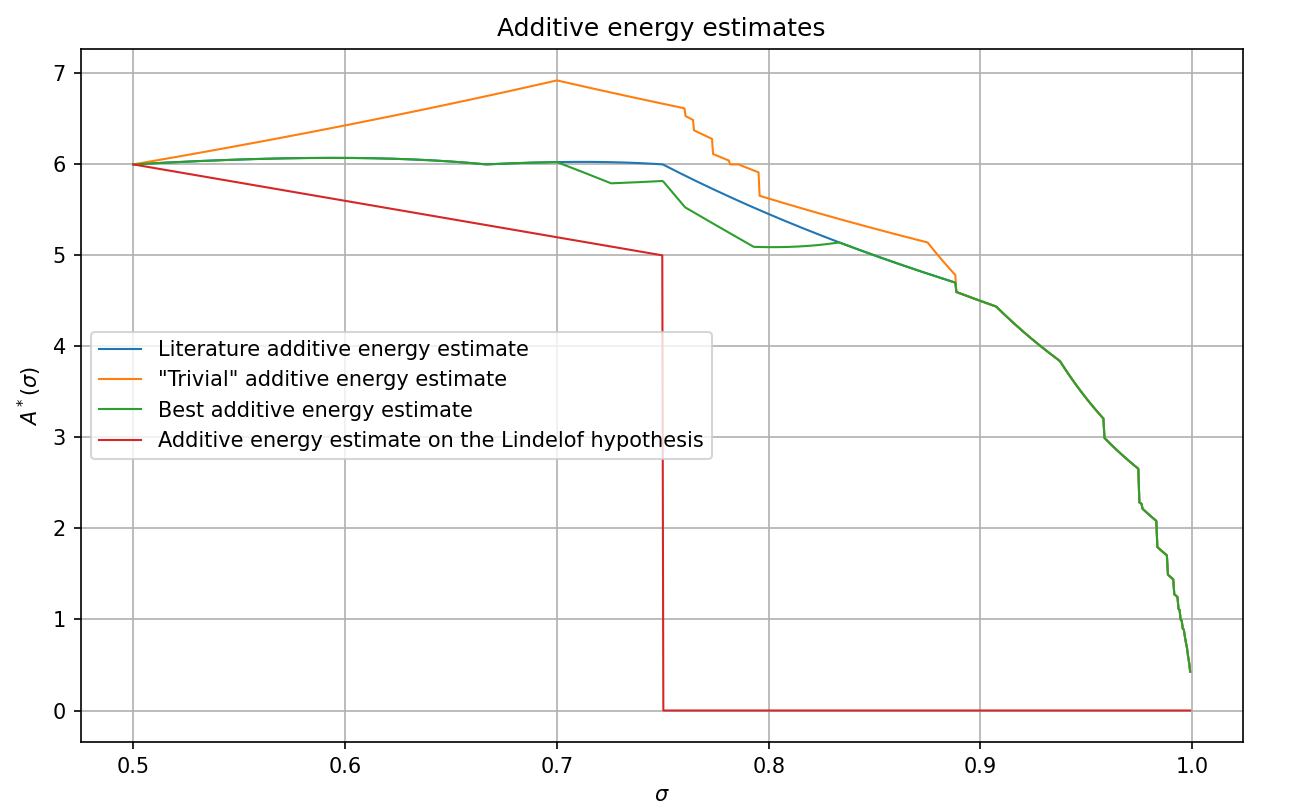
\includegraphics[width=0.5\textwidth]{chapter/zero_density_energy_estimate.png}
    \caption{Comparison of bounds on $\A^*(\sigma)$ under various assumptions.}
    \label{fig:zero_density_energy_estimate}
\end{figure}

\chapter{Zero free region for the zeta function}\label{zerofree-chapter}

\unintegrated 

A zero of the Riemann zeta function is a complex number $\rho = \beta + i\gamma$ for which $\zeta(\rho) = 0$. The zeta function has a infinite number of zeros of the form $\rho = -2n$ for integer $n \ge 1$; these are known as trivial zeros and are well understood. There are also an infinite number zeros inside the ``critical strip" $0 < \Re z < 1$, called non-trivial zeros. The locations of the non-trivial zeros have deep consequences for many fields of mathematics. A well-known conjecture regarding the non-trivial zeros is the Riemann hypothesis. 

\begin{conjecture}[Riemann hypothesis]\label{rh}
If $\rho$ is a non-trivial zero of the Riemann zeta function, then $\Re \rho = 1/2$.
\end{conjecture}

This conjecture remains far out of reach. Instead, currently what are known are zero free regions.  

\begin{definition}[Zero free region]\label{zeta-zero-free-def}
A zero-free region of the Riemann zeta function is a set $D \subset \mathbb{C}$ for which $\zeta(s) \ne 0$ for all $s \in D$. 
\end{definition}

\begin{lemma}[Basic properties of zero free regions]\label{zero-free-basic-lem}
The following properties hold:
\begin{enumerate}
    \item[(i)] (Symmetry about the real axis) If $\zeta(\sigma + it) \ne 0$ then $\zeta(\sigma - it) \ne 0$.
    \item[(ii)] (Symmetry about the critical line $\Re s = 1/2$) For $0 \le \sigma \le 1$, if $\zeta(\sigma + it) \ne 0$ then $\zeta(1 - \sigma + it) \ne 0$.
    \item[(iii)] (Non vanishing for $\Re s > 1$) If $\Re s > 1$ then $\zeta(s) \ne 0$.
\end{enumerate}
\end{lemma}
\begin{proof}
Claim (i) follows directly from the property $\overline{\zeta(s)} = \zeta(\overline{s})$. Claim (ii) follows from the functional equation 
\[
\zeta(s) = 2^s \pi^{s - 1}\sin(\pi s/2) \Gamma(1 -s)\zeta(1-s)
\]
and claim (iii) follows from the Euler product formula
\[
\zeta(s) = \prod_{p}(1 - p^{-s})^{-1},\qquad (\Re s > 1).
\]
\end{proof}

In light of \Cref{zero-free-basic-lem}, for the rest of the chapter we will focus on the quadrant 
\[
D\subseteq \{z \in \mathbb{C}: \Re z > 1/2, \Im z > 0\}.
\]
The first non-trivial zero-free region was due to de la Vall\'ee Poussin \cite{de_la_vallee_poussin_recherches_1896} and Hadamard \cite{hadamard_distribution_1896}, who showed independently that:


\begin{theorem}[Non-vanishing on the 1-line]
One has $\zeta(1 + it) \ne 0$ for any real $t$.
\end{theorem}
\begin{proof}
For $\Re s > 1$, one has
\[
\Re \log \zeta(s) = \sum_{p}\sum_{m = 1}^{\infty}\frac{\cos (t \log p^m)}{mp^{m\sigma}}
\]
where the outer sum runs through all primes. Applying this formula at $s = \sigma, \sigma + it$ and $\sigma + 2it$ ($t \ne 0$), and since $3 + 4\cos\theta + \cos 2\theta = 2(1 + \cos\theta)^2 \ge 0$, one has
\[
3\Re \log \zeta(\sigma) + 4\Re \log \zeta(\sigma + it) + \Re\log \zeta(\sigma + 2it) = \sum_{p}\sum_{m = 1}^{\infty}\frac{3 + \cos (t \log p^m) + \cos (2t\log p^m)}{mp^{m\sigma}} \ge 0.
\]
It follows that $|\zeta(\sigma)^3 \zeta(\sigma + it)^4 \zeta(\sigma + 2it)| \ge 1$. Now as $\sigma \to 1$ from above (and $t$ remains fixed), one has
\[
\zeta(\sigma) \ll \frac{1}{\sigma - 1},\qquad \zeta(\sigma + 2it) \ll 1,
\]
since $\zeta$ has a simple pole at $s = 1$ and no pole at $\sigma + 2it$. If $\zeta(1 + it) = 0$, then $\zeta(\sigma + it) \ll \sigma - 1$ so that $|\zeta(\sigma)^3 \zeta(\sigma + it)^4 \zeta(\sigma + 2it)| \ll \sigma - 1$, a contradiction.
\end{proof}

This was used to prove the prime number theorem $\pi(x) \sim x/\log x$ as $x \to \infty$ (in fact the two statements are equivalent).

\section{Relation to upper bound on zeta in the critical strip}

Using estimates of $\zeta(\sigma + it)$ close to the line $\sigma = 1$, one can extend the zero free region slightly inside the critical strip. 

\begin{lemma}[Relation to growth exponents of zeta]\label{mu_to_zero_free}
Suppose $f(t) > 0$ and $0 < g(t) \le 1$ are real-valued functions for $t \ge 0$, with $f(t)$ non-decreasing and tending to infinity with $t$, and $g(t)$ non-increasing. Suppose further that $f(t)/g(t) = o(\exp(f(t)))$. If 
\[
\zeta(\sigma + it) \ll \exp(f(t))\qquad (1 - g(t) \le \sigma \le 2, t \ge 0)
\]
then $\zeta(\sigma + it) \ne 0$ for 
\[
\sigma \ge 1 - A\frac{g(2t + 1)}{f(2t + 1)}
\]
where $A > 0$ is an absolute constant. 
\end{lemma}
\begin{proof}
See \cite[Theorem 3.10]{titchmarsh_theory_1986}.
\end{proof}

\begin{theorem}[Classical zero free region]\label{zfr-classical}
One has $\zeta(\sigma + it) \ne 0$ if 
\[
\sigma \ge 1 - \frac{A}{\log t}.
\]
for an absolute constant $A > 0$ and $t$ sufficiently large.
\end{theorem}
\begin{proof}
Apply \Cref{mu_to_zero_free} with $g(t) = 1/2$, $f(t) = \log (t + 2)$ and the convexity bound $\mu(\sigma) \le (1-\sigma)/2$.
\end{proof}

This classical result has been improved in a number of works, most of which make crucial use of non-trivial estimates of certain types of exponential sums.

\begin{theorem}[Littlewood zero free region]\label{zfr-littlewood}
One has $\zeta(\sigma + it) \ne 0$ if 
\[
\sigma \ge 1 - \frac{A \log\log t}{\log t}
\]
for an absolute constant $A > 0$ and $t$ sufficiently large.
\end{theorem}
\begin{proof}
Follows from the zeta bound corresponding to
\[
\mu(1 - \frac{k}{2^k - 2}) \le \frac{1}{2^k - 2}
\]
for integer $k\ge 3$, which is generated by the van der Corput exponent pair $A^{k - 2}B(0, 1) = (\frac{1}{2^k - 2}, 1 - \frac{k - 1}{2^k - 2})$. However, one needs to make explicit the $o(1)$ term in the bound $\zeta(\sigma + it) \ll t^{\mu(\sigma) + o(1)}$. In particular, by \cite[Theorem 5.14]{titchmarsh_theory_1986}, one has 
\[
\zeta(1 - \frac{k}{2^k - 2} + it) \ll t^{1/(2^k - 2)}\log t.
\]
Taking 
\[
k = \left\lfloor \frac{1}{\log 2}\log\left(\frac{\log t}{\log\log t}\right)\right\rfloor
\]
and using the Phragm\'en Lindel\"of principle, one has 
\[
\zeta(\sigma + it) \ll (\log t)^5,\qquad (\sigma \ge 1 - \frac{(\log\log t)^2}{\log t}),
\]
so we may take $f(t) = 5\log\log t$ and $g(t) = (\log\log t)^2/\log t$ in \Cref{mu_to_zero_free}.
\end{proof}

\begin{theorem}[Chudakov zero free region]\label{zfr-chudakov}
One has $\zeta(\sigma + it) \ne 0$ if 
\[
\sigma \ge 1 - \frac{1}{(\log t)^{3/4 + o(1)}}
\]
for $t$ sufficiently large.
\end{theorem}

\begin{theorem}[Korobov-Vinogradov zero free region]\label{zfr-vk}
One has $\zeta(\sigma + it) \ne 0$ if 
\[
\sigma \ge 1 - \frac{A}{(\log t)^{2/3}(\log\log t)^{1/3}}
\]
for an absolute constant $A > 0$ and $t$ sufficiently large.
\end{theorem}

\section{Relation to the error term in the prime number theorem}

\begin{lemma}[Relation to prime number theorem error term]\label{zero_free_to_pnt}
Suppose $\zeta(\sigma + it) \ne 0$ for $\sigma \ge 1 - \eta(t)$ where $\eta(t)$ is a positive and decreasing function. Then
\[
\sum_{n \le x}\Lambda(n) - x \ll x \exp\left(-A \omega(x) \right),\qquad (x \to \infty)
\]
for an absolute constant $A > 0$, where 
\[
\omega(x) := \inf_{t \ge 1}(\eta (t) \log x + \log t).
\]
\end{lemma}
\begin{proof}
See e.g. \cite{ingham_distribution_1990}.
\end{proof}

Applying \Cref{zero_free_to_pnt}, one obtains the error term estimates in the prime number theorem given in Table \ref{zero-free-pnt-table}.   

\begin{table}[ht]
    \def\arraystretch{2.5}
    \centering
    \caption{Error bounds on the prime number theorem. Here $A$ represents an absolute, positive constant, which may be different at each occurrence.}
    \begin{tabular}{|c|c|c|}
    \hline
    Bound on $(\psi(x) - x)/x$ & Associated zero-free region & Reference \\
    \hline
    $\exp(-A(\log x)^{1/2})$ & $\sigma \ge 1 - \dfrac{A}{\log t}$ & \Cref{zfr-classical} \\
    \hline 
    $\exp(-A(\log x \log\log x)^{1/2})$ & $\sigma \ge 1 - \dfrac{A\log\log t}{\log t}$ & \Cref{zfr-littlewood} \\
    \hline 
    $\exp\left(-A\dfrac{(\log x)^{3/5}}{(\log\log x)^{1/5}}\right)$ & $\sigma \ge 1 - \dfrac{A}{(\log t)^{2/3}(\log\log t)^{1/3}}$ & \Cref{zfr-vk} \\
    \hline 
    \end{tabular}
\label{zero-free-pnt-table}
\end{table}
\chapter{Distribution of primes: long ranges}
\label{chap:prime_counting_function}

Let $\Lambda(n)$ denote the von Mangoldt function, i.e. $\Lambda(n) = \log p$ if $n = p^m$ where p is prime and $m$ is a positive integer, and $\Lambda(n) = 0$ otherwise. 

\begin{definition}
For all $x \ge 1$ define the Chebyshev prime counting functions $\psi(x)$, $\theta(x)$ and $\pi(x)$ as
\[
\psi(x) := \sum_{n \le x}\Lambda(n),\qquad \theta(x) := \sum_{p \le x}\log p,\qquad \pi(x) := \sum_{p \le x}1
\]
where the first sum is over positive integers $n$ and the last two sums are over primes $p$.
\end{definition}

These functions, particularly $\pi(x)$, are central to number theory because they measure the distribution of prime numbers among the integers. A well-known result is the prime number theorem.

\begin{theorem}[Prime number theorem]
As $x \to \infty$, 
\[
\pi(x) \sim \frac{x}{\log x} \sim \operatorname{li}(x) := \int_2^{\infty}\frac{dt}{\log t}.
\]
\end{theorem}

The following are equivalent formulations of the prime number theorem.

\begin{theorem}[Prime number theorem, alternative formulations]
As $x \to \infty$, one has $\psi(x) \sim x$ and $\theta(x) \sim x$.
\end{theorem}

\section{Error bounds for prime counting functions}
In addition to their asymptotic behaviour, various bounds on the deviation from their respective asymptotics are known. The current best-known error bounds are derived from zero-free regions of the Riemann zeta function $\zeta(s)$. The relation between zeroes of $\zeta(s)$ and error bounds for prime counting functions are illustrated through von Mangoldt's explicit formula: for all non-integer $x > 0$, one has
\[
\psi(x) = x - \sum_{\rho}\frac{x^\rho}{\rho} - \log 2\pi - \frac{1}{2}\log(1 - x^{-2}),
\]
where $\rho$ runs through all non-trivial zeroes of $\zeta(s)$.

\begin{theorem}[Korobov--Vinogradov estimate]
There exists a positive constant $A$, such that
\begin{align*}
\psi(x) - x, \; \theta(x) - x, \; \pi(x) - \operatorname{li}(x) \ll x\exp\left(-A\frac{(\log x)^{3/5}}{(\log\log x)^{1/5}}\right).
\end{align*}
\end{theorem}

\Cref{prime-error-table} lists the historical progression on estimates of $\pi(x)$.

\begin{table}[ht]
    \caption{Historical estimates of $\pi(x)$, for $x$ sufficiently large.}
    \centering
    \renewcommand{\arraystretch}{2.2}
    \begin{tabular}{|c|c|}
    \hline
    Reference & Estimate of $\pi(x)$\\
    \hline
    Chebyshev & $c_1 \dfrac{x}{\log x} \leq \pi(x) \leq c_2 \dfrac{x}{\log x}$ for some constants $0 < c_1 < 1 < c_2$, i.e. $\pi(x) \asymp \dfrac{x}{\log x}$\\
    \hline
    de la Vall\'{e}e Poussin \cite{de_la_vallee_poussin_recherches_1896}, Hadamard \cite{hadamard_distribution_1896} & $\pi(x) = \dfrac{x}{\log x}(1 + o(1))$ i.e. $\pi(x) \sim \dfrac{x}{\log x}$\\
    \hline
    de la Vall\'{e}e Poussin \cite{de_la_vallee_poussin_fonction_1899} & $\pi(x) = \operatorname{li}(x) + O(x\exp(-A\sqrt{\log x}))$ for some $A > 0$\\
    \hline
    Littlewood \cite{littlewood_researches_1922} & $\pi(x) = \operatorname{li}(x) + O(x\exp(-A\sqrt{\log x\log\log x}))$ for some $A > 0$\\
    \hline 
    Korobov, Vinogradov \cite{vinogradov_eine_1958} & $\pi(x) = \operatorname{li}(x) + O\left(x\exp\left(-\dfrac{A(\log x)^{3/5}}{(\log\log x)^{1/5}}\right)\right)$ for some $A > 0$\\
    \hline
    \end{tabular}\label{prime-error-table}
\end{table}

Under the Riemann hypothesis, stronger error bounds are known. 
\begin{theorem}[\cite{koch_sur_1901}]
If the Riemann hypothesis is true, then
\[
\psi(x) - x,\; \theta(x) - x \ll x^{1/2}(\log x)^2,\qquad \pi(x) - \operatorname{li}(x) \ll x^{1/2}\log x.
\]
\end{theorem}

Slightly sharper estimates are possible if one assumes even stronger hypotheses. 
\begin{theorem}[Heath-Brown \cite{heathbrown_gaps_1982}]
Assume that the Riemann hypothesis is true. Furthermore, assume that 
\[
F_T(X) := \sum_{0 < \gamma_1, \gamma_2 \le T}\frac{e((\gamma_1 - \gamma_2)X)}{1 + (\gamma_1 - \gamma_2)^2/4} = o(T^2 (\log T)^2)
\]
where the sum is over the imaginary parts of all pairs of non-trivial zeroes of $\zeta(s)$. Then
\[
\psi(x) = x + o(x^{1/2}(\log x)^2).
\]
\end{theorem}
The same result was previously proved (assuming stronger hypotheses) by Gallagher--Mueller \cite{gallagher_primes_1978} and later by Mueller. 

\section{Relation to zero free region of zeta}

\begin{lemma}[Relation to zero free regions]\label{zero_free_to_pnt}\cite{ingham_distribution_1990}
Suppose $\zeta(\sigma + it) \ne 0$ for $\sigma \ge 1 - \eta(t)$ where $\eta(t)$ is a positive and decreasing function. Then
\[
\psi(x) - x \ll x \exp\left(-A \omega(x) \right)\qquad (x \to \infty)
\]
for an absolute constant $A > 0$, where 
\[
\omega(x) := \inf_{t \ge 1}(\eta (t) \log x + \log t).
\]
\end{lemma}

Applying \Cref{zero_free_to_pnt}, one obtains the error term estimates in the prime number theorem given in Table \ref{zero-free-pnt-table}.   

\begin{table}[ht]
    \def\arraystretch{2.5}
    \centering
    \caption{Zero free regions for $\zeta(s)$, along with the bound on $\psi(x) - x$ that they imply. Here $A$ represents an absolute, positive constant, which may be different at each occurrence.}
    \begin{tabular}{|c|c|c|}
    \hline
    Reference & Zero free region & Bound on $(\psi(x) - x)/x$ \\
    \hline
    \Cref{zfr-classical} & $\sigma \ge 1 - \dfrac{A}{\log t}$ & $\exp(-A(\log x)^{1/2})$ \\
    \hline 
    \Cref{zfr-littlewood} & $\sigma \ge 1 - \dfrac{A\log\log t}{\log t}$ & $\exp(-A(\log x \log\log x)^{1/2})$\\
    \hline 
    \Cref{zfr-chudakov} & $\sigma \ge 1 - \dfrac{A}{(\log t)^{3/4 + o(1)}}$ & $\exp(-A(\log x)^{4/7 + o(1)})$\\
    \hline 
    \Cref{zfr-vk} & $\sigma \ge 1 - \dfrac{A}{(\log t)^{2/3}(\log\log t)^{1/3}}$ & $\exp\left(-A\dfrac{(\log x)^{3/5}}{(\log\log x)^{1/5}}\right)$\\
    \hline 
    \end{tabular}
\label{zero-free-pnt-table}
\end{table}

The following type of converse statement is also known.

\begin{theorem}[\cite{turan_new_1984} Theorem 40.1] If for some $0 < \alpha \le 1$ one has
\[
\psi(x) - x \ll x \exp(-A(\log x)^{1/(1 + \alpha)})\qquad (x \to \infty)
\]
then $\zeta(\sigma + it) \ne 0$ for $t$ sufficiently large and
\[
\sigma > 1 - \frac{A}{(\log t)^{\alpha}}.
\]
Here $A$ denotes an absolute positive constant, not necessarily the same at each occurrence. 
\end{theorem}


\section{Omega results}

In the opposite direction, it is known that 
\begin{theorem}[Schmidt \cite{schmidt_uber_1903}]
As $x \to \infty$,
\[
\psi(x) = x + \Omega(x^{1/2}).
\]
\end{theorem}
This can be improved slightly conditioned on the Riemann hypothesis.
\begin{theorem}[Littlewood \cite{littlewood_sur_1914}]
If the Riemann hypothesis is true, then as $x \to \infty$,
\[
|\pi(x) - \operatorname{li}(x)| = \Omega\left(x^{1/2}\frac{\log\log\log x}{\log x}\right).
\]
\end{theorem}

Furthermore it is also known that
\begin{theorem}[Grosswald \cite{grosswald_sur_1965}]
If 
\[
\theta = \sup_{\rho: \zeta(\rho) = 0}\Re \rho > 1/2
\]
then as $x \to \infty$,
\[
\psi(x) = x + \Omega(x^{\theta}).
\]
\end{theorem}


\chapter{Distribution of primes: short ranges}\label{primes-sec}

Recall that $\Lambda$ is the von Mangoldt function, and that the prime number theorem asserts that
$$ \sum_{n \leq x} \Lambda(n) = x + o(x)$$
for unbounded $x$.  If $p_n$ denotes the $n^{\mathrm{th}}$ prime, the prime number theorem is also equivalent to
$$ p_n = (1+o(1)) n \log n$$
for unbounded $n$.

We now consider local versions of the prime number theorem.

\begin{definition}[Prime number theorem in short interval exponents]\label{pnt-ap}
    \begin{itemize}
        \item[(i)] We let $\PNTALL$ denote the least exponent with the following property: if $\eps > 0$ is fixed, and $x$ is unbounded, then
        $$ \sum_{x \leq n < x+y} \Lambda(n) = y + o(y)$$
        whenever $x^{\PNTALL + \eps} \leq y \leq x^{1-\eps}$.
        \item[(ii)] We let $\PNTAA$ denote the least exponent with the following property: if $\eps > 0$ is fixed, and $X$ is unbounded, then we have
        $$ \int_X^{2X} |\sum_{x \leq n < x+y} \Lambda(n)-y|\ dx = o(Xy)$$
        whenever $X^{\PNTAA + \eps} \leq y \leq X^{1-\eps}$.
        \item[(iii)] We let $\GAPMAX$ denote the least exponent such that, if $p_n$ denotes the $n^{\mathrm{th}}$ prime, that
        $$ p_{n+1} - p_n \ll n^{\GAPMAX+o(1)} = p_n^{\GAPMAX+o(1)}$$
        as $n \to \infty$.
        \item[(iv)] We let $\GAPSQUARE$ denote the least exponent such that
        $$ \sum_{p_n \leq x} (p_{n+1}-p_n)^2 \ll x^{\GAPSQUARE+o(1)}$$
        as $x \to \infty$.
        \item[(v)] We let $\GAPAA$ denote the least exponent such that for every $\eps>0$, the intervals $[n, n^{\GAPAA+\eps}]$ contain a prime for a density $1$ set of natural numbers $n$.
    \end{itemize}
\end{definition}

\begin{lemma}[Trivial bounds]\label{pnt-triv}\uses{pnt-ap}
    We have
    $$ 0 \leq \GAPAA \leq \PNTAA, \GAPMAX \leq \PNTALL \leq 1$$
    and $1 \leq \GAPSQUARE \leq 1+\GAPMAX$.
\end{lemma}

\begin{proof} These are all immediate, after noting from the prime number theorem that $\sum_{p_n \leq x} p_{n+1} - p_n = x^{1+o(1)}$.
\end{proof}

The Cram\'er random model \cite{cramer} predicts

\begin{conjecture}[Prime gap conjecture]\uses{pnt-ap} $\PNTALL = 0$, and hence (by Lemma \ref{pnt-triv}) $\GAPAA = \PNTAA = \GAPMAX=0$ and $\GAPSQUARE=1$.
\end{conjecture}

We note that the results of Maier \cite{maier-primes} show that there is some deviation from the prime number theorem at very small scales (of order $\log^{O(1)} x$), but this does not directly affect the exponents discussed here due to the epsilons in our definitions.

A basic connection with zero density exponents is

\begin{proposition}[Zero density theorems and prime gaps]\label{prime-gap}  Let
\begin{equation}\label{A-def}
    \|\A\|_\infty := \sup_{1/2 \leq \sigma \leq 1} A(\sigma).
\end{equation}
Then
    $$ \PNTALL \leq 1 - \frac{1}{\|\A\|_\infty}$$
    and
    $$ \PNTAA \leq 1 - \frac{2}{\|\A\|_\infty}.$$
\end{proposition}

\begin{proof} See for instance \cite[\S 13.2]{guth-maynard}.
\end{proof}

\begin{corollary}[Ingham-Huxley bound]\uses{pnt-ap}  We have $\PNTALL \leq \frac{7}{12}$ and $\PNTAA \leq \frac{1}{6}$.
\end{corollary}

\begin{proof}\uses{prime-gap, thm:ingham_zero_density2, huxley-bound}  From Theorem \ref{thm:ingham_zero_density2} and Theorem \ref{huxley-bound} one as $\|\A\|_\infty \leq 12/5$, and the claim now follows from Proposition \ref{prime-gap}.
\end{proof}

\begin{corollary}[Ingham-Guth-Maynard bound]\cite{guth-maynard}\uses{pnt-ap}  We have $\PNTALL \leq \frac{17}{30}$ and $\PNTAA \leq \frac{2}{15}$.
\end{corollary}

These are currently the best known upper bounds on $\PNTALL$ and $\PNTAA$.

\begin{proof}\uses{prime-gap, thm:ingham_zero_density2, guth-maynard-density}  From Theorem \ref{thm:ingham_zero_density2} and Theorem \ref{guth-maynard-density} one as $\|\A\|_\infty \leq 30/13$, and the claim now follows from Proposition \ref{prime-gap}.
\end{proof}

\begin{corollary}\uses{pnt-ap}  The density hypothesis implies that $\PNTALL \leq 1/2$ and $\PNTAA = 0$.
\end{corollary}

The current unconditional best bound on $\GAPMAX$ is

\begin{theorem}\cite{lu_yuan_primes_2025}\label{bhp-thm}\uses{pnt-ap} We have $\GAPMAX \leq 259/500 = 0.518$.
\end{theorem}

Historical bounds on $\GAPMAX$ are summarized in the following table:

\begin{table}[ht]
    \caption{Historical upper bounds on $\GAPMAX$.}
    \centering
    \renewcommand{\arraystretch}{1.2}
    \begin{tabular}{|c|c|}
    \hline
    Reference & Upper bound \\
    \hline
    Hoheisel (1930) \cite{hoheisel_1930} & $1 - \frac{1}{33000} = 0.999\dots$ \\
    \hline
    Heilbronn (1933) \cite{heilbronn_1933} & $1 - \frac{1}{250} = 0.996$ \\
    \hline
    Ingham (1937) \cite{ingham_difference_1937} & $\frac{5}{8} = 0.625$ \\
    \hline
    Montgomery (1969) \cite{montgomery_1969} & $\frac{3}{5} = 0.6$ \\
    \hline
    Huxley (1972) \cite{Huxley} & $\frac{7}{12} = 0.5833\dots$ \\
    \hline
    Iwaniec--Jutila (1979)\cite{iwaniec-jutila} & $\frac{13}{23} = 0.5652\dots$ \\
    \hline
    Heath-Brown--Iwaniec (1979) \cite{heathbrown_iwaniec_1979}, Lou--Yao (1993) \cite{lou_yao_number_1993}& $\frac{11}{20} = 0.55$ \\
    \hline
    Pintz (1981) \cite{pintz_1981} & $\frac{17}{31} = 0.5483\dots$ \\
    \hline
    Iwaniec--Pintz (1984) \cite{iwaniec-pintz} & $\frac{23}{42} = 0.5476\dots$\\
    \hline
    Mozzochi (1986) \cite{mozzochi-consecutive} & $\frac{1051}{1920} = 0.5473\dots$ \\
    \hline
    Lou--Yao (1992) \cite{lou-yao-chebychev} & $\frac{6}{11} = 0.5454\dots$\\
    \hline
    Baker-Harman (1996) \cite{baker-harman} & $\frac{107}{200} = 0.535$\\
    \hline
    Baker--Harman--Pintz (2001) \cite{baker-harman-pintz} & $\frac{21}{40} = 0.525$ \\
    \hline
    R. Li (2025) \cite{li_number_2025} & $\frac{13}{25} = 0.52$\\
    \hline
    Lu--Yuan (2025) \cite{lu_yuan_primes_2025} & $\frac{259}{500} = 0.518$\\
    \hline
    \end{tabular}
    \end{table}\label{gapmax-table}

Bounds on $\GAPAA$ are recorded in Table \ref{gapaa-table}.

\begin{table}[ht]
    \caption{Historical upper bounds on $\GAPAA$.}
    \centering
    \renewcommand{\arraystretch}{1.2}
    \begin{tabular}{|c|c|}
    \hline
    Reference & Upper bound \\
    \hline
    Selberg (1943) \cite{selberg_1943} & $\frac{19}{77}=0.2467\dots$\\
    \hline
    Montgomery (1971) \cite{montgomery_topics_1971} & $\frac{1}{5}=0.2$ \\
    \hline
    Huxley (1972) \cite{Huxley} & $\frac{1}{6} = 0.1666\dots$ \\
    \hline
    Harman (1982) \cite{harman_1982} & $\frac{1}{10} = 0.1$ \\
    \hline
    Harman (1983) \cite{harman_1983}, Heath-Brown (1983) \cite{heathbrown_sieve_1984}  & $\frac{1}{12} = 0.0833\dots$ \\
    \hline
    Jia (1995) \cite{jia_goldbach_1994} & $\frac{1}{13} = 0.0769\dots$ \\
    \hline
    Lou--Yao (1985) \cite{lou_yao_1985} & $\frac{17}{227}= 0.0748\dots$ \\
    \hline
    H. Li (1995) \cite{li_goldbach_1995} & $\frac{2}{27} = 0.0740\dots$ \\
    \hline
    Jia (1995) \cite{jia_difference_1995}, Watt (1995) \cite{watt_short_1995} & $\frac{1}{14}=0.0714\dots$ \\
    \hline
    H. Li (1997) \cite{li_short_1997} & $\frac{1}{15}=0.0666\dots$ \\
    \hline
    Baker--Harman--Pintz (1997) \cite{baker-harman-pintz_goldbach_1997} & $\frac{1}{16} = 0.625$ \\
    \hline
    Wong (1996) \cite{wong_thesis_1996}, Jia (1996) \cite{jia_exceptional_1996}, Harman (2007) \cite{harman-book} & $\frac{1}{18} = 0.0555\dots$ \\
    \hline
    Jia (1996) \cite{jia_almost_all} & $\frac{1}{20} = 0.05$ \\
    \hline
    R. Li (2024) \cite{li_primes_almost_2024} & $\frac{2}{43} = 0.0465\dots$ \\
    \hline
    \end{tabular}
    \end{table}\label{gapaa-table}

    Historical bounds on $\GAPSQUARE$ are recorded in Table \ref{gapsquare-table}.

    \begin{table}[ht]
        \caption{Historical upper bounds on $\GAPSQUARE$.}
        \centering
        \renewcommand{\arraystretch}{1.2}
        \begin{tabular}{|c|c|}
        \hline
        Reference & Upper bound \\
        \hline
        Selberg (1943) \cite{selberg_1943} & $1$ (on RH)\\
        \hline
        Heath-Brown (1978) \cite{heath_brown_consecutive_I} & $\frac{4}{3} = 1.3333\dots$\\
        \hline
        Heath-Brown (1979) \cite{heath_brown_consecutive_II} & $\frac{7}{6} = 1.1666\dots$ (on LH) \\
        \hline
        Heath-Brown (1979) \cite{heath_brown_consecutive_II} & $\frac{1413}{1067} = 1.3242\dots$ \\
        \hline
        Heath-Brown (1979) \cite{heath_brown_consecutive_III} & $\frac{23}{18} = 1.2777\dots$ \\
        \hline
        Yu (1996) \cite{yu_differences_1996} & $1$ (on LH) \\
        \hline
        Peck (1996) \cite{peck_on_1996}, Maynard (2012) \cite{maynard_difference_2012} & $\frac{5}{4} = 1.25$ \\
        \hline
        Stadlmann (2022) \cite{stadlmann_mean_2022} & $\frac{123}{100} = 1.23$ \\
        \hline
    \end{tabular}
    \end{table}\label{gapsquare-table}

The following general bound on $\GAPSQUARE$ is known:

\begin{proposition}\label{gapsquare-from-a}\uses{pnt-ap, zero-def, zeroe-def}
    We have
    $$ \GAPSQUARE \leq \max\left( 2-\frac{2}{\|\A\|_\infty}, \sup_{1/2 \leq \sigma \leq 1} \max(\alpha(\sigma), \beta(\sigma))\right)$$
    where
    $$ \alpha(\sigma) := 4\sigma - 2 + 2 \frac{B(\sigma)(1-\sigma)-1}{B(\sigma)-A(\sigma)}$$
    and
    $$ \beta(\sigma) := 4\sigma - 2 + \frac{B(\sigma)(1-\sigma)-1}{A(\sigma)}$$
    where $A(\sigma), B(\sigma)$ are any upper bounds for $\A(\sigma), \A^*(\sigma)$ respectively.
\end{proposition}

\begin{proof} See \cite[Lemma 2]{heath_brown_consecutive_II}. We remark that this lemma allows $\sigma$ to range over $0 \leq \sigma \leq 1$ rather than $1/2 \leq \sigma \leq 1$, but it is easy to see that the contributions of the $0 \leq \sigma < 1/2$ cases are dominated by the $\sigma=1/2$ case.
\end{proof}

\code{compute_gap2()}


This proposition can be used to recover the following bounds on $\GAPSQUARE$:

\begin{corollary}\
    \begin{itemize}
    \item[(i)] Assuming the Riemann hypothesis, $\GAPSQUARE = 1$. (Selberg, 1943 \cite{selberg_1943})
    \item[(ii)] Assuming the Lindelof hypothesis, $\GAPSQUARE \leq 7/6$. (Heath-Brown, 1979 \cite{heath_brown_consecutive_II})
    \item[(iii)] Unconditionally, $\GAPSQUARE \leq 23/18$. (Heath-Brown, 1979 \cite{heath_brown_consecutive_III}).
\end{itemize}
\end{corollary}

\begin{proof}\uses{gapsquare-from-a, lindelof_implies_density, zeroe-lindelof, hb-energy-bound} For (i), we observe that $\|A\|_\infty=2$ and that one can take $A(\sigma)=B(\sigma)=\eps$ for any $\sigma>1/2$ and $\eps>0$, and $A(\sigma)=2$, $B(\sigma)=6$ for $\sigma=1/2$, and then the claim follows from Proposition \ref{gapsquare-from-a}.

For (ii), from Theorem \ref{lindelof_implies_density} we may take $A(\sigma)=2$ for $\sigma \leq 3/4$ and $A(\sigma)=\eps$ for $3/4 < \sigma \leq 1$ and any $\eps>0$, while from Theorem \ref{zeroe-lindelof} one can take $B(\sigma) = 8-4\sigma$ for $\sigma \leq 3/4$ and $B(\sigma)=\eps$ for $3/4 < \sigma \leq 1$.  The claim now follows from Proposition \ref{gapsquare-from-a} and a routine calculation.

Part (iii) follows from applying Proposition \ref{gapsquare-from-a} using the bounds from Theorem \ref{hb-energy-bound}, together and various bounds on $\A(\sigma)$; see \cite[Theorem 12.14]{ivic} for details.
\end{proof}

Two variants of $\GAPSQUARE$ are $\GAPLARGE$ and $\GAPLARGEEQ$, defined respectively as the least exponent for which
$$ \sum_{p_n \leq x: p_{n+1}-p_n \geq x^{1/2+\eps}} (p_{n+1}-p_n) \ll x^{\GAPLARGE+o(1)}$$
(for any fixed $\eps>0$ for unbounded $x \geq 1$) and
$$ \sum_{p_n \leq x: p_{n+1}-p_n \geq x^{1/2}} (p_{n+1}-p_n) \ll x^{\GAPLARGEEQ+o(1)}$$
(for unbounded $x \geq 1$).  The trivial bounds are

\begin{proposition}[Trivial bounds on large gaps]\label{trivial-large-gap}  One has $\GAPLARGE \le \GAPLARGEEQ$. If $\GAPMAX < 1/2$, then $\GAPLARGE = -\infty$.  In general, we have
    $$ \max(1/2,\GAPMAX) \leq \max(1/2, \GAPLARGE)$$
    and $\GAPLARGE \leq 1$.  Also $\GAPLARGE \leq \GAPSQUARE - 1/2$.
\end{proposition}

The proofs are routine and are omitted.  Historical bounds on $\GAPLARGE$ are recorded in Table \ref{gaplarge-table}.

\begin{table}[ht]
    \caption{Historical upper bounds on $\GAPLARGE$ and $\GAPLARGEEQ$.}
    \centering
    \renewcommand{\arraystretch}{1.2}
    \begin{tabular}{|c|c|c|}
    \hline
    Reference & Upper bound on $\GAPLARGE$ & Upper bound on $\GAPLARGEEQ$\\
    \hline
    Selberg (1943) \cite{selberg_1943} & $\frac{1}{2}=0.5$ (on RH) & \\
    \hline
    Wolke (1975) \cite{wolke_1975} & & $\frac{29}{30} = 0.966\dots$ \\
    \hline
    Cook (1979) \cite{cook_1979} & $\frac{85}{98} = 0.8673\dots$ & \\
    \hline
    Huxley (1980) \cite{huxley_large_1980} & $\frac{1759}{2134} = 0.8242\dots$ & \\
    \hline
    Huxley (1980) \cite{huxley_large_1980} & $\frac{3}{4} = 0.75$ (on LH) & \\
    \hline
    Iv\'ic (1979) \cite{ivic_sums_1979} & $\frac{215}{266} = 0.8082\dots$ & \\
    \hline
    Heath-Brown (1979) \cite{heath_brown_consecutive_III} & & $\frac{3}{4} = 0.75$ \\
    \hline
    Heath-Brown (1979) \cite{heath_brown_consecutive_II} & $\frac{5}{8} = 0.625$ & \\
    \hline
    Peck (1998) \cite{peck_differences_1998} & & $\frac{25}{36} = 0.6944\ldots$ \\
    \hline
    Matom\"{a}ki (2007) \cite{matomaki_large_2007} & & $\frac{2}{3} = 0.6666\ldots$ \\
    \hline
    Heath-Brown (2020) \cite{heath-brown_differences_2021} & & $\frac{3}{5} = 0.6$\\
    \hline
    J\"{a}rviniemi (2022) \cite{jarviniemi_large_2022} & & $\frac{57}{100} = 0.57$\\
    \hline
    \end{tabular}
\end{table}\label{gaplarge-table}

For any $0 < \theta < 1$, let $\PNTEXCEP(\theta)$ denote the least exponent $\mu$ such that for all unbounded $X$, one has $\sum_{x \leq n < x + x^\theta} \Lambda(n) = (1+o(1)) x^\theta$ for all $x \in [X,2X]$ outside of an exceptional set of measure $O(X^{\mu+o(1)})$.  Thus for instance $\PNTEXCEP(\theta)=-\infty$ for $\theta > \PNTALL$ (and $\PNTEXCEP(\theta) \geq 0$ for $\theta < \PNTALL$), and $\PNTEXCEP(\theta) < 1$ implies $\theta \geq \PNTAA$. The quantity $\PNTEXCEP(\theta)$ is clearly non-decreasing in $\theta$.

The following bounds are known:

\begin{lemma}[Bounds on $\mu$]\label{baz-bound}\
  \begin{itemize}
  \item[(i)]  \cite[Theorem 2(i)]{bazzanella-perelli}  For sufficiently small $\Delta>0$, we have $\PNTEXCEP(1/6 + \Delta) \leq 1 - c\Delta$ and $\PNTEXCEP(7/12-\Delta) \leq \frac{5}{8} + \frac{7}{4}\Delta + O(\Delta^2)$.
  \item[(ii)] \cite[Theorem 2(ii)]{bazzanella-perelli} Assuming RH, we have $\PNTEXCEP(\theta) \leq 1-\theta$ for $0 < \theta \leq 1/2$.
    \item[(iii)] \cite[Lemma 1]{bazzanella} We have
  $$
  \PNTEXCEP(\theta) \leq
  \begin{cases}
  \frac{3(1-\theta)}{2} & \frac{1}{2} < \theta \leq \frac{11}{21} \\
  \frac{47-42\theta}{35}& \frac{11}{21} < \theta \leq \frac{23}{42} \\
  \frac{36\theta^2-96\theta+55}{39-36\theta} & \frac{23}{42} < \theta \leq \frac{7}{12} \\
  \end{cases}
  $$
  Some further bounds were claimed in the region $1/6 < \theta \leq 1/2$, but unfortunately the arguments provided are incomplete (the claim (13) of that paper is not justified for $\theta \leq 1/2$).
  \item[(iv)] \cite{gafni-tao} For any $0 < \theta < 1$, one has
$$\PNTEXCEP(\theta) \leq \inf_{\eps>0} \sup_{\stackrel{0 \leq \sigma < 1}{\A(\sigma) \geq \frac{1}{1-\theta}-\eps}} \min(\mu_{2,\sigma}(\theta), \mu_{4,\sigma}(\theta))$$
where
$$ \mu_{2,\sigma}(\theta) := (1-\theta)(1-\sigma) \A(\sigma) + 2\sigma - 1$$
and
$$ \mu_{4,\sigma}(\theta) := (1-\theta)(1-\sigma) \A^*(\sigma) + 4\sigma-3.$$
  \end{itemize}
\end{lemma}

\code{prime_excep()}



\section{Extremal values of prime gaps}

Consider now the problem of determining upper bounds on
\begin{equation}\label{eqn:small-prime-gaps}
H_1 := \liminf_{n\to\infty}(p_{n + 1} - p_n)
\end{equation}
as well as lower bounds on
\begin{equation}\label{eqn:large-prime-gaps}
G(X) := \max_{p_{n + 1} \le X}(p_{n + 1} - p_n).
\end{equation}
From the prime number theorem one expects $p_{n + 1} - p_n$ to be of size $\log p_n$ on average, so that
\begin{theorem}[Consequences of the prime number theorem]
One has
\[
\liminf_{n\to\infty}\frac{p_{n + 1} - p_n}{\log p_n} \le 1,\qquad G(X) \ge (1 + o(1)) \log X\quad (X \to \infty).
\]
\end{theorem}

However, $p_{n + 1} - p_n$ can be sometimes be much smaller or much larger than its average size. The following is a classical conjecture regarding small prime gaps.

\begin{conjecture}[Twin prime conjecture]
One has
\[
\liminf_{n\to\infty}(p_{n + 1} - p_n) = 2.
\]
\end{conjecture}

Since all sufficiently large primes are odd, the twin prime conjecture states that prime gaps achieve the smallest possible size, infinitely often. In the other direction, it is conjectured that
\begin{conjecture}[Cram\'er \cite{cramer}]
One has
\[
\limsup_{X \to \infty}\frac{G(X)}{(\log X)^2} = 1.
\]
\end{conjecture}
Note that by \Cref{bhp-thm} it is known that $G(X) \ll X^{0.518}$.

The current best known result concerning \eqref{eqn:small-prime-gaps} is
\begin{theorem}[Polymath 8b \cite{polymath_variants_2014}]
One has
\[
\liminf_{n\to\infty}(p_{n + 1} - p_n) \le 246.
\]
\end{theorem}

Sharper conditional bounds are also known.
\begin{theorem}[Maynard \cite{maynard_small_2015}]
Assuming the Elliott-Halberstam conjecture (EH), one has
\[
\liminf_{n\to\infty}(p_{n + 1} - p_n) \le 12.
\]
\end{theorem}
\begin{theorem}[Polymath 8b \cite{polymath_variants_2014}]
Assuming the Generalized Elliott-Halberstam conjecture (GEH), one has
\[
\liminf_{n\to\infty}(p_{n + 1} - p_n) \le 6.
\]
\end{theorem}
Historical progress towards this problem is recorded in \Cref{small-primegap-table}.

\begin{table}[ht]
    \caption{Historical progression of bounds related to \eqref{eqn:small-prime-gaps}.}
    \centering
    \renewcommand{\arraystretch}{2.2}
    \begin{tabular}{|c|c|c|}
    \hline
    Reference & Unconditional result & Assuming EH \\
    \hline
    Goldston--Pintz--Yıldırım (2009) \cite{goldston_primes_2009} & $\displaystyle\liminf_{n\to\infty}\frac{p_{n + 1} - p_n}{\log p_n} = 0$ & $H_1 \le 16$ \\
    \hline
    Goldston--Pintz--Yıldırım (2010) \cite{goldston_primes_2010} & $\displaystyle\liminf_{n\to\infty}\frac{p_{n + 1} - p_n}{(\log p_n)^{1/2}(\log\log p_n)^2} < \infty$ & \\
    \hline
    Pintz (2013) \cite{} & $\displaystyle\liminf_{n\to\infty}\frac{p_{n + 1} - p_n}{(\log p_n)^{3/7}(\log\log p_n)^{4/7}} < \infty$ & \\
    \hline
    Zhang (2014) \cite{zhang_bounded_2014} & $H_1 < 7\cdot 10^7$ & \\
    \hline
    Polymath 8a (2014) \cite{castryck_new_2014} & $H_1 \le 4680$ & \\
    \hline
    Maynard (2015) \cite{maynard_small_2015} & $H_1 \le 600$ & $H_1 \le 12$ \\
    \hline
    Polymath 8b (2015) \cite{polymath_variants_2014} & $H_1 \le 246$ & \\
    \hline
    \end{tabular}
\end{table}\label{small-primegap-table}

The current best known lower bound on $G(X)$ is
\begin{theorem}[Ford--Green--Konyagin--Maynard--Tao (2017) \cite{ford_long_2017}]
For unbounded $X$, one has
\[
G(X) \gg \frac{\log X \log \log X \log\log\log \log X}{\log \log \log X}
\]
\end{theorem}
\begin{table}[ht]
    \caption{Historical progression of bounds related to \eqref{eqn:large-prime-gaps}.}
    \centering
    \renewcommand{\arraystretch}{2.2}
    \begin{tabular}{|c|c|c|}
    \hline
    Reference & Lower bound on $G(X)$ (for $X$ sufficiently large) \\
    \hline
    Westzynthius (1931) \cite{westzynthius_uber_1931} & $\displaystyle G(X) \gg \log X \frac{\log\log\log X}{\log\log\log\log X}$\\
    \hline
    Erdős (1935) \cite{erdos_difference_1935} & $\displaystyle G(X) \gg \log X \frac{\log\log X}{(\log\log\log X)^2}$ \\
    \hline
    Rankin (1938) \cite{rankin_difference_1938} & $\displaystyle G(X) > (c_0 + o(1))\log X \frac{\log \log X \log \log \log \log X}{(\log \log \log X)^2}$ with $c_0 = 1/3$ \\
    \hline
    Sch\"{o}nhage (1963) \cite{schonhage_bemerkung_1963} & $c_0 = \dfrac{1}{2}e^\gamma$\\
    \hline
    Rankin (1963) \cite{rankin_difference_1963} & $c_0 = e^\gamma$ \\
    \hline
    Maier--Pomerance (1990) \cite{maier_unusually_1990} & $c_0 = 1.31256 e^\gamma$\\
    \hline
    Pintz (1997) \cite{pintz_very_1997} & $c_0 = 2e^\gamma$\\
    \hline
    Ford--Green--Konyagin--Tao (2016) \cite{ford_large_2016}, Maynard (2016) \cite{maynard_large_2016} & $\displaystyle G(X) \gg f(X)\log X \frac{\log \log X \log \log \log \log X}{(\log \log \log X)^2}$ for some $f(X) \to \infty$\\
    \hline
    Ford--Green--Konyagin--Maynard--Tao (2017) \cite{ford_long_2017} & $\displaystyle G(X) \gg \frac{\log X \log \log X \log\log\log \log X}{\log \log \log X}$ \\
    \hline
\end{tabular}
\end{table}\label{small-primegap-table2}

\chapter{The generalized Dirichlet divisor problem}

\begin{definition}[Divisor sum exponents]\label{divisor-def} Let $k \geq 1$ be an integer. Then, $\alpha_k$ is the best exponent for which one has the asymptotic
$$ \sum_{n \leq x} d_k(n) = x P_{k-1}(\log x) + O(x^{\alpha_k+o(1)})$$
as $x \to \infty$, where $P$ is an explicit polynomial of degree $k-1$ and $d_k(n) := \sum_{n_1 \dots n_k=n} 1$ is the $k^{\mathrm{th}}$ divisor function. The implied constant may depend on $k$. 
\end{definition}

In the case $k = 1$, the problem is trivial. In particular:

\begin{lemma}[$d_1$ exponent]\label{divisor-1}\uses{divisor-def} One has $\alpha_1=0$.
\end{lemma}
\begin{proof}
Follows from $\sum_{n \le x}1 = x + O(1)$. 
\end{proof}

On the other hand, the value of $\alpha_k$ is an open problem for all $k \ge 2$. Unconditionally, the following lower-bound on $\alpha_k$ is known to hold. 

\begin{lemma}[Lower bound on $\alpha_k$]\label{divisor-lower}\uses{divisor-def}
For all $k \geq 1$, one has
\[
\alpha_k \geq \frac{1}{2} - \frac{1}{2k}.
\]
\end{lemma}
\begin{proof} See Hardy \cite{hardy_divisor_1916}.
\end{proof}

Multiple authors {\bf [give cite]} have refined Hardy's result but only in the $o(1)$ term in the exponent. It is conjectured that this lower bound on $\alpha_k$ is in fact an equality \cite[p.\ 320]{titchmarsh_theory_1986}. Amongst other consequences, this conjecture implies the Lindel\"of hypothesis \cite[Chapter XII]{titchmarsh_theory_1986}.  
\begin{conjecture}[Generalised Dirichlet divisor problem conjecture]
For all $k \geq 1$, one has
\[
\alpha_k = \frac{1}{2} - \frac{1}{2k}.
\]
\end{conjecture}

The remainder of this chapter focuses on upper bounds on $\alpha_k$. 

\section{Known bounds on $\alpha_2$}

Currently the sharpest known upper bound on $\alpha_2$ is:

\begin{theorem}\label{divisor-2-bound}\cite[Theorem 1.2]{li_yang_gauss_2024}\uses{divisor-def} One has $\alpha_2 \leq \alpha^* = 0.314483\ldots$, where $\alpha^*$ is the solution to the equation
\[
\frac{8}{25}\alpha - \frac{(\sqrt{2(1+14\alpha)} - 5\sqrt{-1+8\alpha})^2}{200} + \frac{51}{200} = \alpha
\]
on the interval $\alpha \in [0.3, 0.35]$.
\end{theorem}

\Cref{div-alpha2-table} records the historical progression of upper bounds on $\alpha_2$.

\begin{table}[ht]
    \def\arraystretch{1.2}
    \centering
    \caption{Historical bounds on $\alpha_2$}
    \begin{tabular}{|c|c|}
    \hline
    Reference & Upper bound on $\alpha_2$\\
    \hline
    Piltz & $1/2 = 0.5$\\
    \hline
    Voronoi (1903) \cite{voronoi_sur_1903} & $1/3 = 0.3333\ldots$\\
    \hline
    van der Corput (1922) \cite{van_der_corput_verscharfung_1922} & $33/100 = 0.33$\\
    \hline
    van der Corput (1928) \cite{van_der_corput_zum_1928} & $27/82 = 0.3292\ldots$\\
    \hline 
    Chih (1950) \cite{chih_on_1950}, Richert (1953) \cite{richert_verschrfung_1953} & $15/46 = 0.3260\ldots$\\
    \hline 
    Kolesnik (1969) \cite{kolesnik_improvement_1969} & $12/37 = 0.3243\ldots$\\
    \hline 
    Kolesnik (1973) \cite{kolesnik_1973} & $346/1067 = 0.3242\ldots$\\
    \hline 
    Kolesnik (1982) \cite{kolesnik_order_1982} & $35/108 = 0.3240\ldots$\\
    \hline 
    Huxley (2003) \cite{huxley_exponential_2003} & $131/416 = 0.3149\ldots$\\
    \hline 
    Li--Yang (2024) \cite{li_yang_gauss_2024} & $0.314483\ldots$\\
    \hline 
    \end{tabular}
\label{div-alpha2-table}
\end{table}


\section{Known bounds on $\alpha_3$}

Currently, the sharpest known bound on $\alpha_3$ is:

\begin{theorem}\label{divisor-kolesnik}\cite{kolesnik}\uses{divisor-def} One has $\alpha_3 \leq 43/96$.
\end{theorem}

\Cref{div-alpha3-table} records the historical progression of upper bounds on $\alpha_3$.

\begin{table}[ht]
    \def\arraystretch{1.2}
    \centering
    \caption{Historical bounds on $\alpha_3$}
    \begin{tabular}{|c|c|}
    \hline
    Reference & Upper bound on $\alpha_3$\\
    \hline
    Walfisz (1926) \cite{walfisz_uber_1926} & $43/87 = 0.4942\ldots$\\
    \hline
    Atkinson (1941) \cite{atkinson_divisor_1941} & $37/75 = 0.4933\ldots$\\
    \hline
    Rankin (1955) \cite{rankin_van_1955} & $0.4931466\ldots$\\
    \hline
    Y\"{u}h (1958) \cite{yuh_divisor_1958} & $14/29 = 0.4827\ldots$\\
    \hline 
    Yin (1959) \cite{} & $25/52 = 0.4807\ldots$\\
    \hline 
    Yin (1959) \cite{} & $10/21 = 0.4761\ldots$\\
    \hline
    Y\"{u}h--Wu (1962) \cite{yuh_wu_divisor_1962} & $8/17 = 0.4705\ldots$\\
    \hline 
    Yin (1964) \cite{} & $34/75 = 0.4533\ldots$\\
    \hline
    Chen (1965) \cite{chen_divisor_1965} & $5/11 = 0.4545\ldots$\\
    \hline
    Yin--Li (1981) \cite{}, Zheng (1988) \cite{} & $127/282 = 0.4503\ldots$\\
    \hline
    Kolesnik (1981) \cite{kolesnik} & $43/96 = 0.4479\ldots$\\
    \hline
    \end{tabular}
\label{div-alpha3-table}
\end{table}






\section{Known bounds on $\alpha_k$ for large $k$}
For larger $k$, estimates typically make use of the following relationship with zeta-moments. 

\begin{lemma}\label{mas}\uses{divisor-def,zeta-moment-def}  Let $k \geq 2$ be an integer. If $M(\sigma,k) = 1$ then $\alpha_k \leq \sigma$.
\end{lemma}

\begin{proof}  See \cite[\S 13.3]{ivic}.
\end{proof}

For completeness we record the historical progression in bounds for $\alpha_k$.  
\begin{lemma}[Piltz bound]For $k \ge 2$, one has
\[
\alpha_k \le 1 - \frac{1}{k}.
\]
\end{lemma}
\begin{lemma}[Voronoi, Landau bound]
For $k \ge 2$, one has
\[
\alpha_k \leq 1 - \frac{2}{k + 1}.
\]
\end{lemma}
\begin{proof}
See Voronoi \cite{voronoi_sur_1903} for $k = 2$ and Landau \cite{landau_uber_1912} for $k \ge 3$. 
\end{proof}

\begin{lemma}[Hardy--Littlewood bound for $k \ge 4$]
For $k \ge 4$, one has
\[
\alpha_k \leq 1 - \frac{3}{k + 2}.
\]
\end{lemma}
\begin{proof}
See \cite{hardy_littlewood_approximate_1923}. The original proof relied on the assumption that $\mu(1/2) \le 1/6$ which was published later. 
\end{proof}

\begin{lemma}[Tong bound for $4 \le k \le 11$]
One has
\begin{alignat*}{4}
\alpha_4 &\le 1/2,\qquad &&\alpha_5 \le 4/7,\qquad &&\alpha_6 \le 5/8,\qquad &&\alpha_7 \le 71/107\\
\alpha_8 &\le 41/59,\qquad &&\alpha_9 \le 31/43,\qquad &&\alpha_{10} \le 26/35,\qquad &&\alpha_{11}\le 19/25
\end{alignat*}
\end{lemma}
\begin{proof}
See Tong \cite{}.
\end{proof}

\begin{theorem}\cite{heathbrown_mean_1981} For $4 \le k \le 8$, one has 
\[
\alpha_k \leq \frac{3k-4}{4k}.
\]
\end{theorem}

\begin{theorem}[Ivi\'c--Ouellet bound for large $k$]\cite{ivic_ouellet_1989} One has
\begin{align*}
\alpha_{10} \le 27/40,\qquad \alpha_{11} &\le 0.6957,\qquad \alpha_{12} \le 0.7130,\qquad \alpha_{13} \le 0.7306,\\
\alpha_{14} \le 0.7461,\qquad \alpha_{15} &\le 0.75851,\qquad \alpha_{16} \le 0.7691,\qquad \alpha_{17} \le 0.7785,\\
\alpha_{18} \le 0.7868,\qquad \alpha_{19} &\le 0.7942,\qquad \alpha_{20} \le 0.8009.
\end{align*}
\end{theorem}
\begin{theorem}\cite[Theorem 13.12]{ivic}\uses{mas}  One can bound $\alpha_k$ by
    \begin{align*}
        (3k-4)/4k & \hbox{ for } 4 \leq k \leq 8 \\
        35/54 & \hbox{ for } k = 9 \\
        41/60 & \hbox{ for } k = 10 \\
        7/10 & \hbox{ for } k = 11 \\
        (k-2)/(k+2) & \hbox{ for } 12 \leq k \leq 25 \\
        (k-1)/(k+4) & \hbox{ for } 26 \leq k \leq 50 \\
        (31k-98)/32k & \hbox{ for } 51 \leq k \leq 57 \\
        (7k-34)/7k & \hbox{ for } k \geq 58.
    \end{align*}
\end{theorem}

\begin{lemma}[Heath-Brown bound for large $k$]
For any $k \ge 2$, one has
\[
\alpha_k \le 1 - 0.849k^{-2/3}.
\]
\end{lemma}
\begin{proof}
See Heath-Brown \cite{heathbrown_new_2017}.
\end{proof}

\begin{theorem}[\cite{bellotti_generalised_2023}]For integer $k \ge 30$, one has
\[
\alpha_k \leq 1 - 1.421(k - 1.18)^{-2/3}.
\]
Moreover, $\alpha_k \leq 1 - 1.889k^{-2/3}$ for sufficiently large $k$.
\end{theorem}
\chapter{The number of Pythagorean triples}\label{pythagorean-chapter}

\begin{definition}[Pythagorean triple exponent]\label{pythag-def}  Let $\Pythag$ be the least exponent for which one has
$$ P(N) = c N^{1/2} - c' N^{1/3} + N^{\Pythag+o(1)}$$
for unbounded $N$ and some fixed $c,c'$, where $P(N)$ is the number of primitive Pythagorean triples of area no greater than $N$.
\end{definition}

\begin{lemma}\label{pythag-14}\uses{pythag-def} One has $\Pythag \leq 1/4$.
\end{lemma}

\begin{proof} See \cite{wild_1955, duttlinger_schwarz}.  The previous bound $\Pythag \leq 1/3$ was obtained in \cite{lambek_moser}.
\end{proof}

\begin{lemma}\label{exp_pair_to_pythag}\uses{pythag-def, exp-pair-def} If $(k,\ell)$ is an exponent pair, and RH holds, then
$$ \Pythag \leq \max( \frac{1}{3} - \frac{5}{6} \frac{k+\ell-3/2}{4(k+\ell)-7}, \frac{1}{2} - \frac{3}{2}\frac{k+\ell-3/2}{4(k+\ell)-7} )$$
\end{lemma}

\begin{proof} See \cite{menzer} and and \cite[Section 5.10]{trudgian-yang}.
\end{proof}

\begin{lemma}\label{pythag-71-316}\uses{pythag-def} Assuming RH, one has $\Pythag \leq 71/316$.
\end{lemma}

\begin{proof} See \cite[Section 5.10]{trudgian-yang}.
\end{proof}

\chapter{The de Bruijn--Newman constant}\label{debruijn-newman-chapter}

A survey on this topic may be found at \cite{newman-wu-survey}.

Let $H_0 \colon \C \to \C$ denote the function
\begin{equation}\label{hoz}
 H_0(z) := \frac{1}{8} \xi\left(\frac{1}{2} + \frac{iz}{2}\right),
\end{equation}
where $\xi$ denotes the Riemann xi function
\begin{equation}\label{sas}
 \xi(s) := \frac{s(s-1)}{2} \pi^{-s/2} \Gamma\left(\frac{s}{2}\right) \zeta(s)
\end{equation}
and $\zeta$ is the Riemann zeta function.
Then $H_0$ is an entire even function with functional equation $H_0(\overline{z}) = \overline{H_0(z)}$, and the Riemann hypothesis is equivalent to the assertion that all the zeroes of $H_0$ are real.

It is a classical fact (see \cite[p. 255]{titch}) that $H_0$ has the Fourier representation
$$ H_0(z) = \int_0^\infty \Phi(u) \cos(zu)\ du$$
where $\Phi$ is the super-exponentially decaying function
\begin{equation}\label{phidef}
 \Phi(u) := \sum_{n=1}^\infty (2\pi^2  n^4 e^{9u} - 3\pi n^2 e^{5u} ) \exp(-\pi n^2 e^{4u} ).
\end{equation}
The sum defining $\Phi(u)$ converges absolutely for negative $u$ also.  From Poisson summation one can verify that $\Phi$ satisfies the functional equation $\Phi(u) = \Phi(-u)$ (i.e., $\Phi$ is even).

De Bruijn \cite{debr} introduced the more general family of functions $H_t \colon \C \to \C$ for $t \in \R$ by the formula
\begin{equation}\label{htdef}
 H_t(z) := \int_0^\infty e^{tu^2} \Phi(u) \cos(zu)\ du.
\end{equation}
As noted in \cite[p.114]{csv}, one can view $H_t$ as the evolution of $H_0$ under the backwards heat equation $\partial_t H_t(z)= -\partial_{zz} H_t(z)$.
As with $H_0$, each of the $H_t$ are entire even functions with functional equation $H_t(\overline{z}) = \overline{H_t(z)}$.  From results of P\'olya \cite{polya} it is known that $H_t$ has purely real zeroes for some $t$ then $H_{t'}$ has purely real zeroes for all $t'>t$.
De Bruijn showed that the zeroes of $H_t$ are purely real for $t \geq 1/2$.  Strengthening these results, Newman \cite{newman} showed that there is an absolute constant $-\infty < \Lambda \leq 1/2$, now known as the \emph{De Bruijn-Newman constant}, with the property that $H_t$ has purely real zeroes if and only if $t \geq \Lambda$.  The Riemann hypothesis is then clearly equivalent to the upper bound $\Lambda \leq 0$.  Newman conjectured the complementary lower bound $\Lambda \geq 0$, and noted that this conjecture asserts that if the Riemann hypothesis is true, it is only ``barely so''.

Known lower bounds on $\Lambda$ are listed in the tables below.

\begin{table}[ht]
  \caption{Lower bounds on $\Lambda$.}
  \begin{tabular}{|l|l|}
  \hline
  Lower bound on $\Lambda$ & Reference \\
  \hline
  $-\infty$ & Newman 1976 \cite{newman} \\
  $-50$ & Csordas--Norfolk--Varga 1988 \cite{cnv} \\
  $-5$ & te Riele 1991 \cite{tr} \\
  $-0.385$ & Norfolk--Ruttan--Varga 1992 \cite{nrv} \\
  $-0.0991$ & Csordas--Ruttan--Varga 1991 \cite{crv} \\
  \hline
  $-4.379 \times 10^{-6}$ & Csordas--Smith--Varga 1994 \cite{csv} \\
  $-5.895 \times 10^{-9}$ & Csordas--Odlyzko--Smith--Varga 1993 \cite{cosv} \\
  $-2.63 \times 10^{-9}$ & Odlyzko 2000 \cite{odlyzko} \\
  $-1.15 \times 10^{-11}$ & Saouter--Gourdon--Demichel 2011 \cite{saouter} \\
  \hline
  $0$ & Rodgers--Tao 2020 \cite{rodgers-tao} \\
  $0$ & Dobner 2021 \cite{dobner} \\
  \hline
  \end{tabular}
  \end{table}

  The argument of Dobner applies more generally to the Selberg class.

  For upper bounds, we have
  \begin{table}[ht]
    \caption{Upper bounds on $\Lambda$.}
    \begin{tabular}{|l|l|}
    \hline
    Upper bound on $\Lambda$ & Reference \\
    \hline
    $\leq 1/2$ & Newman 1976 \cite{newman} \\
    $< 1/2$ & Ki--Kim--Lee 2009 \cite{kkl} \\
    $\leq 0.22$ & Polymath 2019 \cite{polymath15} \\
    $\leq 0.2$ & Platt--Trudgian 2021 \cite{platt-trudgian} \\
    \hline
  \end{tabular}
\end{table}


% Newly submitted chapters (not integrated with the rest of the blueprint) can go here initially, marked with the `\unintegrated` macro; they can be integrated later.

\chapter{Brun-Titchmarsh type theorems}\label{brun-titchmarsh-chapter}


\begin{definition}[Prime counting function on arithmetic progressions]
Suppose $a,q\in\mathbb Z$ with $\gcd(a,q)=1$. For each $x\geq0$, define
$$\pi(x;q,a)=\sum_{\substack{p\leq x\\p\text{ prime}\\q\mid(p-a)}}1.$$
The ordinary prime counting function can be recovered by $\pi(x)=\pi(x;1,1)$.
\end{definition}

The Prime Number Theorem (PNT) shows that $\pi(x)\sim\frac x{\log x}$ as $x\to\infty$. On the other hand, known results on the asymptotic behavior of $\pi(x;q,a)$ depend greatly on how $q$ and $x$ are sent to $\infty$. Heuristically, it is expected that for ``most'' sequences $q_n,x_n\to\infty$ with $q_n<x_n$, $\pi(x_n;q_n,a)\sim\frac{x_n}{\varphi(q_n)\log(x_n)}$ as $n\to\infty$. Brun-Titchmarsh type theorems make this precise by provide asymptotic upper or lower bounds on $\pi(x;q,a)$ in terms of $\frac x{\varphi(q)\log x}$ or related quantities, presupposing constraints between $q$ and $x$.

\begin{definition}[Logarithmic integral function]
Define the offset logarithmic integral function for $x\geq2$ by $\operatorname{Li}(x)=\int_2^x\frac{\mathrm du}{\log u}$. Note that $\operatorname{Li}(x)\sim\frac x{\log x}$.
\end{definition}

We first record two early results which recover the correct asymptotic under stringent assumptions.

\begin{theorem}[Brun-Titchmarsh theorem under GRH (1929) \cite{titchmarsh_divisor_1930}]\label{titchmarsh-GRH-asymptotic}
Under the Generalized Riemann Hypothesis (GRH), if $q<x$, then
$$\pi(x;q,a)=\frac{\operatorname{Li}(x)}{\varphi(q)}+O(x^{1/2}\log x).$$
\end{theorem}

\begin{theorem}[Walfisz (1936) \cite{walfisz_1936}]\label{walfisz-small-q-asymptotic}
Fix $B\geq0$ and suppose $q\leq(\log x)^B$. Then there exists $A=A(B)>0$ such that
$$\pi(x;q,a)=\frac{\operatorname{Li}(x)}{\varphi(q)}+O(x\exp(-A\sqrt{\log x})).$$
\end{theorem}

\section{Upper bounds}
Titchmarsh's original theorem establishes a coarse asymptotic upper bound.

\begin{theorem}[Brun-Titchmarsh theorem (1929) \cite{titchmarsh_divisor_1930}]
If $0<\theta<1$ and $q\leq x^\theta$, then
$$\pi(x;q,a)=O\left(\frac x{\varphi(q)\log x}\right)+O(x^{6(1-\theta)/7}).$$
\end{theorem}

Later bounds more generally bound the number of prime numbers equivalent to $a\pmod q$ in the interval $[x,x+y]$. Observe that setting $x=0$ indeed yields an improvement on previous results.

\begin{theorem}[Lint, Richert (1965) \cite{lint_richert_1965}]
If $y>q$, then
$$\pi(x+y;q,a)-\pi(x;q,a)<\frac{2y}{\varphi(q)\log(y/q)}\min\left(\frac32,1+\frac6{\log(y/q)}\right).$$
\end{theorem}

\begin{theorem}[Montgomery, Vaughan (1973) \cite{montgomery_vaughan_1973}]
If $y>q$, then
$$\pi(x+y;q,a)-\pi(x;q,a)<\frac{2y}{\varphi(q)\log(y/q)}.$$
\end{theorem}

On the other hand, various bounds improve on this result under polynomial relationships of the form $q\leq x^\theta$. To state these, we need the following definition.
\begin{definition}[$\theta$ and $C_\theta$]
Suppose $x>0$ and $q\in\mathbb Z$. Define $\theta:=\frac{\log q}{\log x}$, and let $C_\theta>0$ be the smallest constant such that
$$\max_{a:\gcd(a,q)=1}\pi(x;q,a)\leq\frac{(C_\theta+o(1))x}{\varphi(q)\log(x)}$$
as $x\to\infty$.
\end{definition}

Here is the historical progression of bounds on $C_\theta$.

\begin{table}[ht]
    \def\arraystretch{1.2}
    \centering
    \caption{Historical bounds on $C_\theta$}
    \begin{tabular}{|c|c|c|}
    \hline
    Reference & Range of $\theta$ & Upper bound on $C_\theta$\\
    \hline
    Titchmarsh (1930) & $(0,1)$ & Finite\\
    \hline
    \begin{tabular}{@{}c@{}} van Lint \& Richert (1965) \cite{lint_richert_1965}\\
    Montgomery \& Vaughan (1973) \cite{montgomery_vaughan_1973}\\
    Selberg (1991) \cite{selberg-collected-II}
    \end{tabular} & $(0,1)$ & $2/(1-\theta)$\\
    \hline
    Motohashi (1973) \cite{motohashi_1973} & $(0,1/3)$ & $16/(8-3\theta)$\\
    \hline
    Motohashi (1974) \cite{motohashi_1974} & $(0,1/3]$ & $2$ (on LH)\\
    \hline
    Motohashi (1973) \cite{motohashi_1973} & $(2/5,1/2]$ & $2/(2-3\theta)$\\
    \hline
    Motohashi (1974) \cite{motohashi_1974} & $[1/3,2/5]$ & $4/(2-\theta)$\\
    \hline
    Motohashi (1974) \cite{motohashi_1974} & $[1/3,2/5]$ & $2/(2-3\theta)$ (on LH)\\
    \hline
    Goldfeld (1975) \cite{goldfeld_1975} & $(0,24/71)$ & $16/(8-3\theta)$\\
    \hline
    Iwaniec (1982) \cite{iwaniec_1982} & $(0,9/20)$ & $16/(8-3\theta)$\\
    \hline
    Iwaniec (1982) \cite{iwaniec_1982} & $(0,9/20)$ & $8/(4-2\theta)$ (if $q$ cube-free)\\
    \hline
    Iwaniec (1982) \cite{iwaniec_1982} & $[9/20,2/3]$ & $8/(6-7\theta)$\\
    \hline
    Baker (1996) \cite{baker} & $(9/20,1/2)$ & $4/(2-\theta)$\\
    \hline
    Friedlander \& Iwaniec (1997) \cite{friedlander_iwaniec_1997} & $[6/11,1)$ & $(2-((1-\theta)/4)^6)/(1-\theta)$\\
    \hline
    Maynard (2013) \cite{maynard_2013} & $(0,1/8]$ & $2$\\
    \hline
    Bourgain \& Garaev (2014) \cite{bourgain_garaev_2014} & $[1-\delta,1)$ & $(2-c_0(1-\theta)^2)/(1-\theta)$\\
    \hline
    Xi \& Zheng (2024) \cite{xi-zheng} & $(9/20,1/2)$ & $16/(8-(3+7/32)\theta)$ \\
    \hline
    Xi \& Zheng (2024) \cite{xi-zheng} & $(9/20,1/2)$ & $16/(8-3\theta)$ (if $q$ prime)\\
    \hline
    Xi \& Zheng (2024) \cite{xi-zheng} & $[1/2,12/23)$ & $8/(5-5\theta)$ (if $q$ prime)\\
    \hline
    Xi \& Zheng (2024) \cite{xi-zheng} & $[12/23,32/61)$ & $32/(32-43\theta)$ (if $q$ prime)\\
    \hline
    Xi \& Zheng (2024) \cite{xi-zheng} & $[32/61,8/15)$ & $24/(16-17\theta)$ (if $q$ prime)\\
    \hline
    Xi \& Zheng (2024) \cite{xi-zheng} & $[8/15,7/13)$ & $48/(40-49\theta)$ (if $q$ prime)\\
    \hline
    Xi \& Zheng (2024) \cite{xi-zheng} & $[7/13,6/11)$ & $16/(11-12\theta)$ (if $q$ prime)\\
    \hline
    Xi \& Zheng (2024) \cite{xi-zheng} & $[6/11,4/7)$ & $32/(28-35\theta)$ (if $q$ prime)\\
    \hline
    Xi \& Zheng (2024) \cite{xi-zheng} & $[9/51,9/11]$ & $160/(89-91\theta)$ (if $q$ smooth square-free)\\
    \hline
    Xi \& Zheng (2024) \cite{xi-zheng} & $[1/8,5/12)$ & $2$ (if $q$ smooth square-free)\\
    \hline
    Xi \& Zheng (2024) \cite{xi-zheng} & $[5/12,9/20)$ & $5/(5-6\theta)$ (if $q$ smooth square-free)\\
    \hline
    Xi \& Zheng (2025) \cite{xi-zheng-2} & $[1/2,34/67]$ & $240/(184-217\theta)$ (if $q$ prime)\\
    \hline
    \end{tabular}
\label{bt-ctheta-table}
\end{table}

Let $\theta_{\mathrm{char}}$ be the least constant such that for every $\eps>0$ there exists $\delta>0$ such that one has a character sum bound of the form
$$ \sum_{l \leq L} \chi(l) \ll L q^{-\delta}$$
whenever $\chi$ is a non-principal character mod $q$ and $L \geq q^{\theta_{\mathrm{char}}}+\eps$.  The Burgess bound \cite{burgess, burgess2} shows that $\theta_{\mathrm{char}} \leq 3/8$, which can be improved to $\theta_{\mathrm{char}} \leq 1/4$ for cube-free $q$.  The extended Lindel\"of hypothesis implies that $\theta_{\mathrm{char}}=0$.

In \cite[Theorem 3]{iwaniec_1982} it was shown that
$$ C_\theta \leq \max( \frac{2}{1 - \theta \theta_{\mathrm{char}}}, \frac{2}{2-12\theta/5}).$$
This was improved in \cite{lou-yao-1986} to
$$ C_\theta \leq \max( \frac{2}{1 - \theta \theta_{\mathrm{char}}}, \frac{2}{8/7-24\theta/35}).$$
A further (complicated) bound on $C_\theta$ in the range $3/7 \leq \theta < 9/20$ may be found in \cite[Theorem 2]{baker}.

In \cite{xi-zheng}, the bound $C_\theta \leq 16/(8-(3+2\theta_{\mathrm{RP}})\theta)$ for $9/20 < \theta < 1/2$ was established, where $\theta_{\mathrm{RP}}$ is the exponent for the Ramanujan--Petersson conjecture for $GL_2(\Q)$.  By the work of Kim and Sarnak \cite{kim2003refined} one has $\theta_{\mathrm{RP}} \leq 7/64$.  One can also convert exponent pairs to bounds on $C_\theta$:

\begin{theorem}[From exponent pairs to Brun--Titchmarsh]\label{convert}\cite[Theorem 1.4]{xi-zheng} If $(k,\ell)$ is an exponent pair, then
    $$ C_\theta \leq \frac{4}{(3+k-\ell) - (3+3k-\ell)\theta}$$
whenever
$$ \frac{1+k-\ell}{2+2k-2\ell} \leq \theta \leq \frac{1+k-\ell}{1+2k-\ell}.$$
\end{theorem}

Averaged versions of the Brun--Titchmarsh inequality were proven in \cite{deshouillers-iwaniec} \cite{mikawa_1991}, \cite{baker-harman-1996}.

For any $\theta$, let $C'_\theta$ denote the best constant for which one has an upper bound
$$\pi(x+x^\theta) - \pi(x) \leq (C'_\theta+o(1)) \frac{x^\theta}{\log x}$$
for unbounded $x$.  The following bounds on $C'_\theta$ are known:
\begin{table}[ht]
    \def\arraystretch{1.2}
    \centering
    \caption{Historical bounds on $C'_\theta$}
    \begin{tabular}{|c|c|c|}
    \hline
    Reference & Range of $\theta$ & Upper bound on $C'_\theta$\\
    \hline
    Montgomery \& Vaughan (1973) \cite{montgomery_vaughan_1973} & $(0,1)$ & $2/\theta$ \\
    \hline
    Iwaniec (1982) \cite{iwaniec_1982} & $(1/3,1)$ & $18/(15\theta-2)$ \\
    \hline
    Iwaniec (1982) \cite{iwaniec_1982} & $(1/2,1)$ & $4/(1+\theta)$ \\
    \hline
    Lou \& Yao (1989) \cite{lou-yao-1989} & $(6/11,11/20]$ & $22/(100\theta-45)$ \\
    \hline
    Lou \& Yao (1992) \cite{lou-yao-chebychev} & $(6/11,1]$ & $1.031$ \\
    \hline
    Baker, Harman, \& Pintz (1997) \cite{baker-harman-pintz_goldbach_1997} & $(0.55,1)$ & $1.0001$ \\
    \hline
    R. Li (2025) \cite{li_number_2025} 
     & $(0.52,0.521]$ & $2.7626$\\
     & $(0.521,0.522]$ & $2.6484$\\
     & $(0.522,0.523]$ & $2.5630$\\
     & $(0.523,0.524]$ & $2.4597$\\
     & $(0.524,0.535]$ & $2.3759$\\
    \hline
    \end{tabular}
\label{bt-ctheta'-table}
\end{table}



\section{Lower bounds}
The most basic lower bound is Dirichlet's theorem, stating that $\lim_{x\to\infty}\pi(x;q,a)=\infty$; we shall not record it here. Until relatively recently, good lower bounds were not known on $\pi(x;q,a)$ other than Theorem \ref{walfisz-small-q-asymptotic} for small $q$, but there are many known estimates for the smallest value of $x$ for which $\pi(x;q,a)>0$.

\begin{definition}[Linnik's constant $L$]
Define $L$ to be the infimum over all $L'>0$ where there exists $q_0(L')>0$ such that for all $q\geq q_0(L')$ and $x>q^{L'}$, $\min_{\gcd(a,q)=1}\pi(x;q,a)>0$.
\end{definition}

Here is the historical progression of $L$.

\begin{table}[ht]
    \def\arraystretch{1.2}
    \centering
    \caption{Historical bounds on $L$}
    \begin{tabular}{|c|c|}
    \hline
    Reference & Upper bound on $L$\\
    \hline
    Linnik (1994) \cite{linnik-1} & $<\infty$\\
    \hline
    Pan (1957) \cite{pan_1957} & $10000$\\
    \hline
    Pan (1958) \cite{pan_1958} & $5448$\\
    \hline
    Chen (1965) \cite{chen_1965} & $777$\\
    \hline
    Jutila (1971) \cite{} & $630$ \\
    \hline
    Jutila (1970) \cite{jutila_1970} & $550$ \\
    \hline
    Chen (1977) \cite{chen_1977} & $168$\\
    \hline
    Jutila (1977) \cite{jutila_1977} & $80$\\
    \hline
    Graham (1977) \cite{graham_1977} & $36$\\
    \hline
    Graham (1981) \cite{graham_1981} & $20$\\
    \hline
    Chen (1979) \cite{chen_1979} & $17$\\
    \hline
    Wang (1986) \cite{wang_1986} & $16$\\
    \hline
    Chen \& Liu (1989) \cite{chen_liu_1989} & $13.5$\\
    \hline
    Chen \& Liu (1990) \cite{chen-liu-v} & $11.5$\\
    \hline
    Wang (1991) \cite{wang_1991} & $8$\\
    \hline
    Heath-Brown (1992) \cite{heath_brown_least_prime} & $5.5$\\
    \hline
    Meng (2000) \cite{meng} & $4.5$ (if $q$ prime)\\
    \hline
    Xylouris (2009) \cite{xylouris_thesis_2009} & $5.2$\\
    \hline
    Xylouris (2011) \cite{xylouris_2011} & $5.18$\\
    \hline
    Xylouris (2011) \cite{xylouris_thesis_2011} & $5$\\
    \hline
    Banks \& Shparlinski (2019) \cite{Banks_Shparlinski_2019} & $\frac{1}{0.4736} = 2.1115\dots$ (if $q$ is a power of a fixed prime)\\
    \hline
    R. Li (2025) \cite{li_number_2025} & $\frac{1}{0.476} = 2.1008\dots$ (if $q$ is a power of a fixed prime)\\
    \hline
    \end{tabular}
\label{bt-l-table}
\end{table}

Recent work by Maynard \cite{maynard_2013} establishes asymptotic lower bounds for $\pi(x;q,a)$.

\begin{theorem}[Maynard (2013) \cite{maynard_2013}]
For sufficiently large $q$ and $x>q^8$, we have
$$\frac{\log q}{q^{1/2}}\left(\frac x{\varphi(q)\log x}\right)\ll\pi(x;q,a).$$
\end{theorem}

\begin{theorem}[Maynard (2013) \cite{maynard_2013}]
Let $\epsilon>0$. There exists $q_0(\epsilon)>0$ such that for all $q\geq q_0(\epsilon)$,
$$\frac{q^{-\epsilon}x}{\varphi(q)\log x}\ll\pi(x;q,a).$$
\end{theorem}

\chapter{Waring and Goldbach type problems, and Schnirelman's constant}\label{waring-goldbach-schnirelman-chapter}

\section{Waring Problem}

\begin{definition}
    Let $A\subset\N$ be such that there exists $k$ for which
    \begin{equation}
        \underbrace{A+A+\cdots+A}_{k\text{ times}}=\N \label{addbasis}
    \end{equation}
    Then $A$ is called an additive basis of $\N$. The minimum $k$ for which \eqref{addbasis} holds is the order of $A$.
\end{definition}

\begin{definition}\label{g(k)}
For any $k\ge1$ let $A_k=\{n^k:n\in\N\cup\{0\}\}$. Let $g(k)$ be the order of $A_k$ when it exists.
That is, $g(k)$ is the minimum number of $k$ powers needed to write any natural number as the sum of (not necessarily unique) $g(k)$ many $k$ powers including 0.
\end{definition}

\begin{definition}\label{G(k)}
For any $k\ge1$, let $G(k)$ be the minimum $m$ such that there exists $N\ge1$ for which
$$\underbrace{A_k+\cdots+A_k}_{m\text{ times}}=\N\setminus J_N.$$
where $J_N=\{1,\dots,N\}$.
That is, $G(k)$ is the minimum number of $k$ powers such that every sufficiently large integer may be written as the sum of (not necessarily unique) $G(k)$ many $k$ powers including 0.
\end{definition}

\subsection{Known values of g(k)}

\begin{theorem}[Lagrange's Four Square Theorem]
We have $g(2)=4$; that is every natural number may be written as the sum of $4$ perfect squares.
\end{theorem}

\begin{theorem}[Linnik \cite{Linnik_Линник1943}]
$g(k)$ exists for all $k\ge1$.
\label{HilbertExistence}
\end{theorem}


Linnik's proof relied on the notion of Schnirelmann density, which will be discussed later.

In fact, the exact value of $g(k)$ is known for almost all $k\ge1$. We have
$$g(k)=2^k+\left[\frac32\right]^k-2\;\;\text{ if }\;\; 2^k\left\{\frac32\right\}^k+\left[\frac32\right]^k\le2^k$$
and, otherwise,
$$g(k)=2^k+\left[\frac32\right]^k+\left[\frac43\right]^k-\xi$$
where $\xi=2$ if $$\left[\frac32\right]^k+\left[\frac43\right]^k+\left[\frac32\right]^k\left[\frac43\right]^k\ge2^k$$
and $3$ otherwise. Note that $[x]$ is the greatest integer less than $x$ and $\{x\}=x-[x]$. It has been shown that there at at most finitely many exceptions \cite{Mahler_1957}. To complete the proof, it suffices to show
$$\left\{\left(\frac32\right)^k\right\}\le1-\left(\frac34\right)^{k-1}$$
It has been shown for all $k > 5000$, $\{(3/2)^k\}\le1-a^{k}$ where $a=2^{-0.9}\approx0.53$, and for sufficiently large $k$, $\{(3/2)^k\}\le1-(0.5769\dots)^{-k}$ \cite{Dubitskas1990ALB} \cite{Bennett_1993}.

\subsection{Known values of $G(k)$}

Only 2 values of $G(k)$ are known definitively: $G(2)=4$ as shown by Lagrange and $G(4)=16$ as shown by Davenport \cite{7dbd7a34-182d-3a8c-ac41-9dfc57f8937a}.

\begin{definition}
    Let $G_1(k)$ be the smallest number $m$ such that
    $$d(\underbrace{A_k+\cdots+A_k}_{m\text{ times}})=1$$
    where $d(A)$ represents the natural density of $A$:
    $$d(A)=\lim_{N\to\infty}\frac{\#(A\cap J_N)}{N}$$
\end{definition}

$G_1(k)$ has been determined for $5$ values:

\begin{table}[ht]
    \def\arraystretch{1.2}
    \centering
    \begin{tabular}{|c|c|}
        \hline
        Davenport \cite{Davenport1939} & $G_1(3)=4$\\
        \hline
        Hardy and Littlewood \cite{Hardy1925} & $G_1(4)=15$\\
        \hline
        Vaughan \cite{Vaughan1986} & $G_1(8)=32$\\
        \hline
        Wooley \cite{wooley_1992} & $G_1(16)=64$\\
        \hline
        Wooley \cite{wooley_1992} & $G_1(32)=128$\\
        \hline
    \end{tabular}
    \caption{Known values of $G_1(k)$}
    \label{tab:G1values}
\end{table}

\subsection{General bounds for $G(k)$}

\begin{theorem}[Brudern and Wooley 2022 \cite{bruedern2022waringsproblemlargerpowers}]
    For all $k\ge1$,
$$G(k)<k(\log k+C_1)+C_2$$
Furthermore,
$$G(k)\le\lceil k(\log k+4.20032)\rceil$$
\label{BW2022}
\end{theorem}

This bound is the sharpest to date and was a significant improvement over the previous bound by Wooley \cite{wooley_1992}: for sufficiently large $k$,
$$G(k)\le k(\log k+\log\log k+2+O(\log\log k/\log k))$$

\subsection{Bounds for special cases for $G(k)$}

\subsubsection{$k=3$}

\begin{lemma} $G(3)\ge4$
\end{lemma}
\begin{proof}
    Note cubes are congruent $1,-1,0$ modulo $9$. Thus, numbers congruent $4,5$ modulo $9$ may not be expressed as the sum of $3$ cubes.
\end{proof}


\begin{theorem}[Linnik \cite{Linnik_1943_sum_cubes}] $G(3)\le7$\end{theorem}


The exact value of $G(3)$ is conjectured to be $4$, but has not been proven.

\subsubsection{Conjectured $G(k)$ for small $k$}

\Cref{tab:Gkforsmallk} summarizes the best upper bounds for $G(k)$ and the conjectured values of $G(k)$ for $7\le k\le 20$.


\begin{table}
    \centering
    \begin{tabular}{|c|c|c|c|c|c|c|c|c|c|l|l|l|l|l|}
        \hline
 & 7& 8& 9& 10& 11& 12& 13& 14&15 & 16& 17&  18&19&20\\
        \hline
         Best Bound&  31&  39&  47&  55&  63&  72&  81&  89&  97& 105& 113&  121&129&137\\
         \hline
         Conjectured&  8&  32&  13&  12&  12&  16&  14&  15&  16& 64& 18&  27&20&25\\
         \hline
    \end{tabular}
    \caption{Conjectured and best upper bounds for $G(k)$ for $7\le k\le 20$}
    \label{tab:Gkforsmallk}
\end{table}

The upper bounds for $k\le13$ were deduced from Wooley \cite{Wooley_2016} and the bounds for $14\le k\le 20$ are from Theorem \ref{BW2022}.

\subsection{Generalized Waring problem and connections to the Generalized Riemann Hypothesis}

Waring's Problem concerns the solvability of equations of the form
\begin{equation}
    x_1^k+x_2^k+\cdots+x_n^k=m \label{eqn1}
\end{equation}
for $m,n,k\in\N$, and Theorem \ref{HilbertExistence} states that for any fixed $k\ge1$, there exists $n\in \N$ such that (\ref{eqn1}) is solvable for all $m\in\N$. A more generalized problem arises when $k$ is not fixed. Given any $\mathbf k=(k_1,\dots,k_n)\in\N^n$, the generalized Waring problem concerns the solvability of the equations of the form
\begin{equation}
    x_1^{k_1}+x_2^{k_2}+\cdots+x_n^{k_n}=m\label{WaringGeneral}
\end{equation}
The following theorem due to Erich Kamke provides a partial result.

\begin{theorem}[Kamke]
    Let $f(x)$ be an integer valued polynomial such that there does not exist $d\in\N$ such that $d|f(n)$ for all $n\in\N$. Then for sufficiently large $k$,
    $$f(x_1)+f(x_2)+\cdots+f(x_k)=m$$
    is solvable for all large enough $m$.
\end{theorem}

Assuming the Generalized Riemann Hypothesis (GRH), The solvability of (\ref{WaringGeneral}) can be guaranteed for specific $\mathbf k$. For example:

\begin{theorem}[Wooley]
    Assuming GRH, then
    \begin{equation}
        x_1^2+x_2^2+x_3^3+x_4^3+x_5^6+x_6^6=n \label{WooleyThm}
    \end{equation}
    is solvable for sufficiently high $n$. Furthermore, (\ref{WooleyThm}) is not solvable for at most $O((\log N)^{3+\epsilon})$ integers between $1$ and $N$.
\end{theorem}

\section{Goldbach-Style Problems}

Goldbach's original conjecture stated that every positive integer could be written as the sum of $3$ primes. In light of Waring's problem, a natural extension of Goldbach's problem asks when
\begin{equation}
    p_1^k+p_2^k+\cdots+p_m^k=n\label{GoldbachEqn}
\end{equation}
is solvable for all $n\in\N$ for $p_1,\dots p_k$ prime and $k\in\N$. It is conjectured when $m\ge k+1$ and for sufficiently large $n$ satisfying local conditions, which will be made more explicit for specific values of $k$, (\ref{GoldbachEqn}) is solvable.

\subsection{When $k=2$}

It is conjectured that
\begin{equation}
n=p_1^2+p_2^2+p_3^2+p_4^2 \label{GoldbachSquares}
\end{equation}
is solvable whenever $n\equiv 4\;(\operatorname{mod}\; 24)$. The following theorem gives the closest solution.

\begin{theorem}[Liu, Wooley, Yu \cite{LIU2004298}]
    Let $E(N)$ be the number of integers $n\equiv 4\;(\operatorname{mod}\; 24)$ for which (\ref{GoldbachSquares}) is not solvable. For any $\epsilon>0$,
    $$E(N)\ll O(N^{\frac38+\epsilon})$$
\end{theorem}

\subsection{When $k=4,5$}

Following Kawada and Wooley, we define the following quantities to give the relevant local conditions for the cases $k=4$ and $k=5$. Let $\theta=\theta(p,k)$ be the greatest power of $p$ dividing $k$; that is $p^\theta|k$ but $p^{\theta+1}\nmid k$. Then, let
\[ \gamma(k,p)=\left\{\begin{matrix}
\theta+2 & \text{ when } p=2, \theta>0  \\
\theta+1 & \text{ otherwise}  \\
\end{matrix}\right\}\]
and
$$K(k)=\prod_{(p-1)|k}p^{\gamma(k,p)}$$
In particular, $K(4)=240$ and $K(5)=2$.

\begin{definition}
    For $k\in\N$, let $H(k)$ be the minimum integer $s$ such that
    $$p_1^k+p_2^k+\cdots+p_s^k=n$$
    is solvable for sufficiently large $n$ whenever $n\equiv s\;(\operatorname{mod}\; K(k))$.
\end{definition}

Finding the value of $H(k)$ is the main focus of the modern Waring-Goldbach problem.

\begin{theorem}[Wooley, Kawada 2001 \cite{kawada_koichi_wooley_trevor_2001}] We have
    \begin{itemize}
        \item $H(4)\le14$
        \item For any positive $A$,
        $$p_1^4+p_2^4+\cdots+p_7^4=n$$
        has at most $O(N(\log N)^{-A})$ exceptions for $n\equiv 7\;(\operatorname{mod}\; 240)$ and $1\le n\le N$.
        \item $H(5)\le21$
        \item For any positive $A$,
        $$p_1^5+p_2^5+\cdots+p_{11}^5=n$$
        has at most $O(N(\log N)^{-A})$ exceptions for $n$ odd and $1\le n\le N$.
    \end{itemize}
\end{theorem}

 In 2014, Zhao improved the bound for $k=4$ and showed $H(4)\le 13$ \cite{Zhao_WaringGoldbach6}. He also showed $H(6)\le 32$ in the same paper.

\subsection{When $k\ge7$}

\begin{theorem}[Kumchev, Wooley 2016 \cite{Kumchev2016}] For large values of $k$,
\begin{equation}
    H(k)\le(4k-2)\log k-(2\log  2-1)k-3
\end{equation}

\Cref{tab:Hkbounds} summarizes the best bounds on $H(k)$ for $7\le k\le20$.

\begin{table}[ht]
    \centering
    \begin{tabular}{|l|c|c|c|c|c|c|c|c|c|l|l|l|c|}
        \hline
          7&8&  9&  10&  11&  12&  13&  14&  15&  16&    17&18&19&20\\
        \hline
          45&57&  69&  81&  93&  107&  121&  134&  149&  163&    177&193&207&223\\
        \hline
        \end{tabular}
    \caption{Upper bounds for $H(k)$}
    \label{tab:Hkbounds}
\end{table}

\end{theorem}

\section{Schnirelmann Density}

\subsection{Existence of Additive Basis}

\begin{definition}
    Define the Schnirelmann density of $A\subset \N$ as
    $$\sigma A=\inf_{n\ge1}\frac{\#(A\cap J_n)}{n}$$
\end{definition}

\begin{definition}
    Define the lower asymptotic density of $A\subset \N$ as
    $$\delta A=\liminf_{n\to\infty}\frac{\#(A\cap J_n)}{n}$$
\end{definition}

\begin{theorem}[Schnirelmann \cite{Schnirelmann1933}]
    Suppose $\sigma A>0$. Then $A$ is an additive basis for $\N$. \label{addbasisthm}
\end{theorem}

With Theorem \ref{addbasisthm}, it is possible to prove many sets form additive bases. For example:

\begin{theorem}[Schnirelmann \cite{Schnirelmann1933}]
    Let $\mathbb P$ denote the set of primes. Then, $\delta(\mathbb P+\mathbb P)>0$. Therefore, $\mathbb P$ is an additive basis for $\N$. The order of $\mathbb P$ is denoted $C$ and called Schnirelmann's constant.
\end{theorem}

Schnirelmann originally bounded $C<80000$ and Helfgott showed in 2013 that $C\le4$ \cite{helfgott2015ternarygoldbachproblem}. Goldbach's conjecture claims that $C=3$.

\begin{theorem}[Romanoff \cite{ASNSP_1995_4_22_4_645_0}]
    Let $\mathfrak S_a=\{p+a^k:p\in\mathbb P, k\in\N\}$. Then, $\sigma\mathfrak S_a>0$ for all $a\in\N$. Thus, each integer $n$ may be written as the sum of at most $C_a$ primes and $C_a$ powers of $a$, where $C_a$ is a constant depending only on $a$.
\end{theorem}


\subsection{Essential Components}

\begin{definition}
    $B\subset \N$ is called an essential component if $\sigma(A+B)>\sigma(A)$ for any $A\subset\N$ with $0<\sigma A<1$.
\end{definition}

Linnik showed in 1933 gave the first example of an essential component that is not a basis \cite{zbMATH03105552}.
Erdos showed in 1936 that every basis is also an essential component \cite{Erdos1935}.
The minimum possible size of an essential component remained an open problem until Ruzsa showed in 1984\cite{Ruzsa_1987} that for any $\epsilon>0$, there exists an essential component $H$ such that
$$\#(H\cap J_n)\ll (\log n)^{1+\epsilon}$$ but there does not exist an essential component such that
$$\#(H\cap J_n)\ll(\log  n)^{1+o(1)}$$

\chapter{The Gauss circle problem and its generalizations}\label{gauss-circle-chapter}

\unintegrated

For any fixed integer $k \ge 2$ and unbounded $R$, consider the problem of estimating the number of integer lattice points contained in $B_k(R)$, a $k$-dimensional ball of radius $R$:
\[
S_k(R) := \# \mathbb{Z}^k \cap B_k(R) = \# \{x \in \mathbb{Z}^k: |x| \le R\}.
\]
Equivalently, $S_k(R)$ may be written as the partial sum 
\[
S_k(R) = \sum_{n \le R^{2}}r_k(n)
\]
where $r_k(n)$ counts the number of integer solutions to the equation $x_1^2 + \cdots + x_k^2 = n$.

By considering the volume of a $k$-dimensional ball of radius $R$, one has the asymptotic
\[
S_k(R) \sim \operatorname{Vol}(B_k(R)) = \frac{\pi^{k/2}}{\Gamma(k/2 + 1)}R^k.
\]
The generalized Gauss circle problem concerns estimating the error term in this approximation. 

\begin{definition}
For fixed integer $k \ge 2$, define $\theta^{\operatorname{Gauss}}_{k}$ as the least (fixed) exponent for which
\[
S_k(R) - \operatorname{Vol}(B_k(R)) \ll R^{\theta^{\operatorname{Gauss}}_{k} + o(1)}.
\]
\end{definition}

\Cref{fig:gauss_circle_2} and \Cref{fig:gauss_circle_3} plots this error term for $k = 2$ and $k = 3$ respectively (for $0 < R \le 1000$).

\begin{figure}
    \centering
    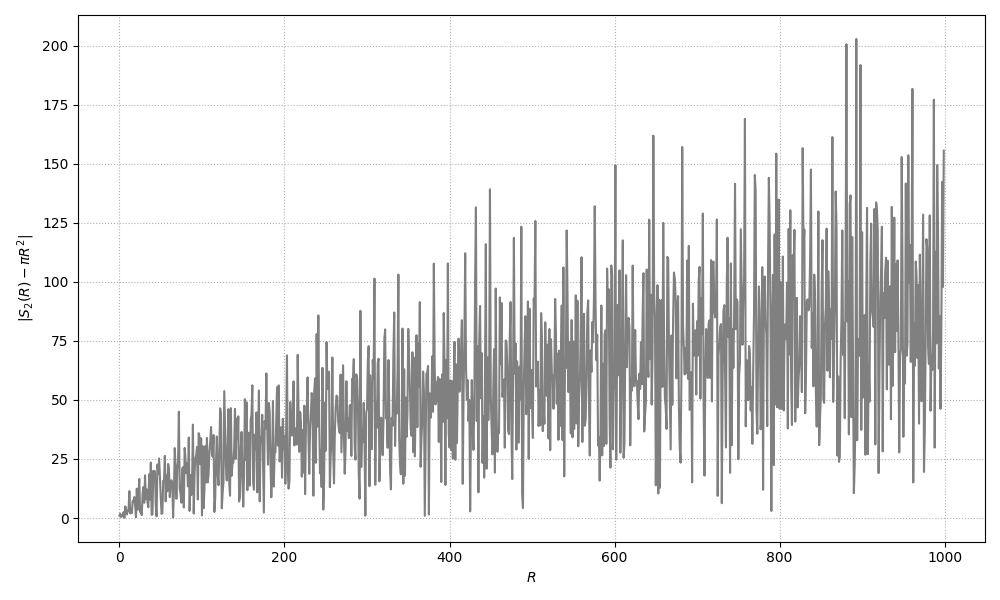
\includegraphics[width=0.5\linewidth]{chapter/gauss_circle_error_2.png}
    \caption{$S_k(R) - \operatorname{Vol}(B_k(R))$ for $k = 2$ and $0 < R \le 1000$}
    \label{fig:gauss_circle_2}
\end{figure}

\begin{figure}
    \centering
    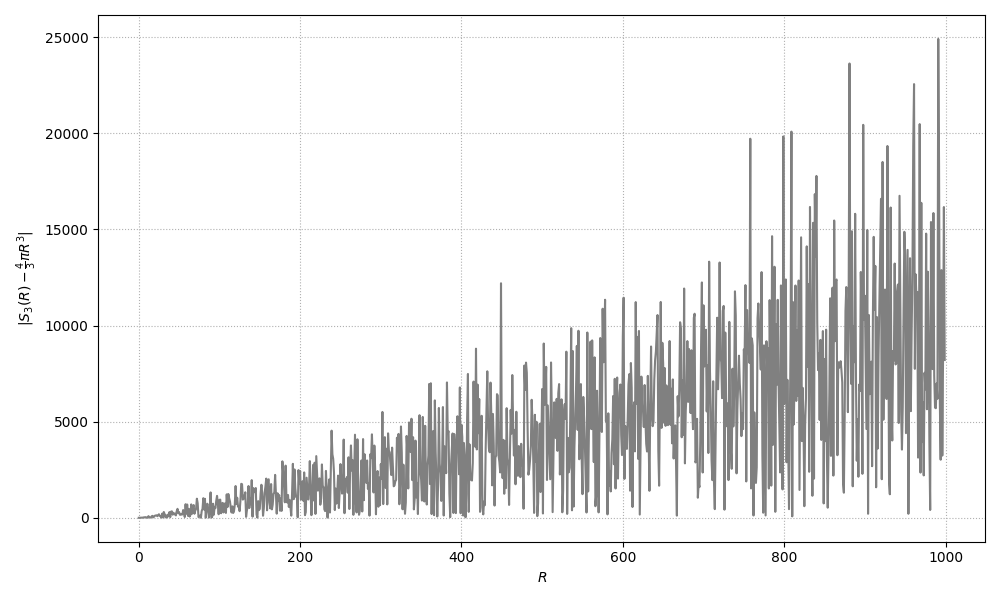
\includegraphics[width=0.5\linewidth]{chapter/gauss_circle_error_3.png}
    \caption{$S_k(R) - \operatorname{Vol}(B_k(R))$ for $k = 3$ and $0 < R \le 1000$}
    \label{fig:gauss_circle_3}
\end{figure}


It is conjectured that 

\begin{conjecture}\label{gauss-circle-conj}
One has 
\[
\theta^{\operatorname{Gauss}}_{k} = \begin{cases}
1/2,& k = 2,\\
k - 2,& k \ge 3.
\end{cases}
\]
\end{conjecture}


\section{Known upper and lower bounds}

\Cref{gauss-circle-conj} is known to hold for $k \ge 4$, i.e.

\begin{theorem}
For integer $k \ge 4$, one has $\theta^{\operatorname{Gauss}}_{k} = k - 2$.
\end{theorem}

The remaining open cases are $k = 2, 3$. For such cases the following lower-bounds on $\theta^{\operatorname{Gauss}}_{k}$ are known:

\begin{theorem}[Hardy \cite{}]\label{gauss-circle-lower-23}
One has $\theta^{\operatorname{Gauss}}_{2} \ge 1/2$ and $\theta^{\operatorname{Gauss}}_{3} \ge 1$.
\end{theorem}

In light of \Cref{gauss-circle-conj} and \Cref{gauss-circle-lower-23}, in the rest of this section we shall focus on upper bounds on $\theta^{\operatorname{Gauss}}_{k}$ for $k = 2, 3$.

The case $k = 2$ is known classically as Gauss's circle problem. The current sharpest known bound on $\theta_2^{\operatorname{Gauss}}$ is
\begin{theorem}[Li--Yang (2023) \cite{li_yang_gauss_2024}] 
One has $\theta_2^{\operatorname{Gauss}} \le 2\alpha$, where $\alpha = 0.31448\ldots$ is the solution to the equation
\[
\frac{8}{25}\alpha - \frac{(\sqrt{2(1+14\alpha)} - 5\sqrt{-1+8\alpha})^2}{200} + \frac{51}{200} = \alpha
\]
on the interval $[0.3, 0.35]$.
\end{theorem}

\begin{remark}
The value of $\alpha$ is the same as that appearing in \Cref{divisor-2-bound}. Historically, methods used to make progress in the $\alpha_2$ exponent in the Dirichlet divisor problem have led to corresponding improvements in $\theta_2^{\operatorname{Gauss}}$ (and vice versa). This may be unsurprising given that both problems reduce to counting the number of lattice points contained in a curved region with a smooth boundary (with the region being the hyperbola $\{(m,n) \in [0, \infty)^2: mn \le x \}$ in the case of the Dirichlet divisor problem).
\end{remark}

The historical progression of upper bounds on $\theta_2^{\operatorname{Gauss}}$ is recorded in \Cref{gauss-circle-table-2}.


\begin{table}[ht]
    \def\arraystretch{1.2}
    \centering
    \caption{Historical upper bounds on $\theta_2^{\operatorname{Gauss}}$}
    \begin{tabular}{|c|c|}
    \hline
    Reference & Bound on $\theta_2^{\operatorname{Gauss}}$\\
    \hline
    Gauss (1834) & $1$\\
    \hline
    Sierpi\'nski (1906) \cite{sierpinski_pewnem_1906} & $2/3 = 0.6666\ldots$\\
    \hline
    van der Corput (1923) \cite{van_der_corput_neue_1923} & $2/3 - \delta$ for some $\delta > 0$\\
    \hline
    Littlewood--Walfisz (1924) \cite{littlewood_lattice_1924} & $37/56 = 0.6607\ldots$\\
    \hline
    Walfisz (1927) \cite{} & $163/247 = 0.6599\ldots$\\
    \hline
    van der Corput (1928) \cite{} & $27/41 = 0.6585\ldots$\\
    \hline
    Titchmarsh (1934) \cite{} & $15/23 = 0.6521\ldots$\\
    \hline
    Hua (1942) \cite{} & $13/20 = 0.65$\\
    \hline
    Iwaniec--Mozzochi (1988) \cite{iwaniec_divisor_1988} & $7/11 = 0.6363\ldots$ \\
    \hline
    Huxley (1993) \cite{} & $46/73 = 0.6301\ldots$\\
    \hline
    Huxley (2003) \cite{huxley_exponential_2003} & $131/208 = 0.6298\ldots$\\
    \hline
    Li--Yang (2023) \cite{li_yang_gauss_2024} & $2\theta^* = 0.6289\ldots$\\
    \hline 
    \end{tabular}
\label{gauss-circle-table-2}
\end{table}




\bibliographystyle{plain} % We choose the "plain" reference style
\bibliography{references}



